\documentclass[]{book}
\usepackage{lmodern}
\usepackage{amssymb,amsmath}
\usepackage{ifxetex,ifluatex}
\usepackage{fixltx2e} % provides \textsubscript
\ifnum 0\ifxetex 1\fi\ifluatex 1\fi=0 % if pdftex
  \usepackage[T1]{fontenc}
  \usepackage[utf8]{inputenc}
\else % if luatex or xelatex
  \ifxetex
    \usepackage{mathspec}
  \else
    \usepackage{fontspec}
  \fi
  \defaultfontfeatures{Ligatures=TeX,Scale=MatchLowercase}
\fi
% use upquote if available, for straight quotes in verbatim environments
\IfFileExists{upquote.sty}{\usepackage{upquote}}{}
% use microtype if available
\IfFileExists{microtype.sty}{%
\usepackage{microtype}
\UseMicrotypeSet[protrusion]{basicmath} % disable protrusion for tt fonts
}{}
\usepackage[margin=1in]{geometry}
\usepackage{hyperref}
\hypersetup{unicode=true,
            pdftitle={Answering questions with data: Lab Manual},
            pdfauthor={Matthew J. C. Crump; Anajali Krishnan; Stephen Volz; Alla Chavarga; Currently in draft, all attributions and licensed to adapted content will be recognized by the time we are finished.},
            pdfborder={0 0 0},
            breaklinks=true}
\urlstyle{same}  % don't use monospace font for urls
\usepackage{natbib}
\bibliographystyle{apalike}
\usepackage{color}
\usepackage{fancyvrb}
\newcommand{\VerbBar}{|}
\newcommand{\VERB}{\Verb[commandchars=\\\{\}]}
\DefineVerbatimEnvironment{Highlighting}{Verbatim}{commandchars=\\\{\}}
% Add ',fontsize=\small' for more characters per line
\usepackage{framed}
\definecolor{shadecolor}{RGB}{248,248,248}
\newenvironment{Shaded}{\begin{snugshade}}{\end{snugshade}}
\newcommand{\KeywordTok}[1]{\textcolor[rgb]{0.13,0.29,0.53}{\textbf{{#1}}}}
\newcommand{\DataTypeTok}[1]{\textcolor[rgb]{0.13,0.29,0.53}{{#1}}}
\newcommand{\DecValTok}[1]{\textcolor[rgb]{0.00,0.00,0.81}{{#1}}}
\newcommand{\BaseNTok}[1]{\textcolor[rgb]{0.00,0.00,0.81}{{#1}}}
\newcommand{\FloatTok}[1]{\textcolor[rgb]{0.00,0.00,0.81}{{#1}}}
\newcommand{\ConstantTok}[1]{\textcolor[rgb]{0.00,0.00,0.00}{{#1}}}
\newcommand{\CharTok}[1]{\textcolor[rgb]{0.31,0.60,0.02}{{#1}}}
\newcommand{\SpecialCharTok}[1]{\textcolor[rgb]{0.00,0.00,0.00}{{#1}}}
\newcommand{\StringTok}[1]{\textcolor[rgb]{0.31,0.60,0.02}{{#1}}}
\newcommand{\VerbatimStringTok}[1]{\textcolor[rgb]{0.31,0.60,0.02}{{#1}}}
\newcommand{\SpecialStringTok}[1]{\textcolor[rgb]{0.31,0.60,0.02}{{#1}}}
\newcommand{\ImportTok}[1]{{#1}}
\newcommand{\CommentTok}[1]{\textcolor[rgb]{0.56,0.35,0.01}{\textit{{#1}}}}
\newcommand{\DocumentationTok}[1]{\textcolor[rgb]{0.56,0.35,0.01}{\textbf{\textit{{#1}}}}}
\newcommand{\AnnotationTok}[1]{\textcolor[rgb]{0.56,0.35,0.01}{\textbf{\textit{{#1}}}}}
\newcommand{\CommentVarTok}[1]{\textcolor[rgb]{0.56,0.35,0.01}{\textbf{\textit{{#1}}}}}
\newcommand{\OtherTok}[1]{\textcolor[rgb]{0.56,0.35,0.01}{{#1}}}
\newcommand{\FunctionTok}[1]{\textcolor[rgb]{0.00,0.00,0.00}{{#1}}}
\newcommand{\VariableTok}[1]{\textcolor[rgb]{0.00,0.00,0.00}{{#1}}}
\newcommand{\ControlFlowTok}[1]{\textcolor[rgb]{0.13,0.29,0.53}{\textbf{{#1}}}}
\newcommand{\OperatorTok}[1]{\textcolor[rgb]{0.81,0.36,0.00}{\textbf{{#1}}}}
\newcommand{\BuiltInTok}[1]{{#1}}
\newcommand{\ExtensionTok}[1]{{#1}}
\newcommand{\PreprocessorTok}[1]{\textcolor[rgb]{0.56,0.35,0.01}{\textit{{#1}}}}
\newcommand{\AttributeTok}[1]{\textcolor[rgb]{0.77,0.63,0.00}{{#1}}}
\newcommand{\RegionMarkerTok}[1]{{#1}}
\newcommand{\InformationTok}[1]{\textcolor[rgb]{0.56,0.35,0.01}{\textbf{\textit{{#1}}}}}
\newcommand{\WarningTok}[1]{\textcolor[rgb]{0.56,0.35,0.01}{\textbf{\textit{{#1}}}}}
\newcommand{\AlertTok}[1]{\textcolor[rgb]{0.94,0.16,0.16}{{#1}}}
\newcommand{\ErrorTok}[1]{\textcolor[rgb]{0.64,0.00,0.00}{\textbf{{#1}}}}
\newcommand{\NormalTok}[1]{{#1}}
\usepackage{longtable,booktabs}
\usepackage{graphicx,grffile}
\makeatletter
\def\maxwidth{\ifdim\Gin@nat@width>\linewidth\linewidth\else\Gin@nat@width\fi}
\def\maxheight{\ifdim\Gin@nat@height>\textheight\textheight\else\Gin@nat@height\fi}
\makeatother
% Scale images if necessary, so that they will not overflow the page
% margins by default, and it is still possible to overwrite the defaults
% using explicit options in \includegraphics[width, height, ...]{}
\setkeys{Gin}{width=\maxwidth,height=\maxheight,keepaspectratio}
\IfFileExists{parskip.sty}{%
\usepackage{parskip}
}{% else
\setlength{\parindent}{0pt}
\setlength{\parskip}{6pt plus 2pt minus 1pt}
}
\setlength{\emergencystretch}{3em}  % prevent overfull lines
\providecommand{\tightlist}{%
  \setlength{\itemsep}{0pt}\setlength{\parskip}{0pt}}
\setcounter{secnumdepth}{5}
% Redefines (sub)paragraphs to behave more like sections
\ifx\paragraph\undefined\else
\let\oldparagraph\paragraph
\renewcommand{\paragraph}[1]{\oldparagraph{#1}\mbox{}}
\fi
\ifx\subparagraph\undefined\else
\let\oldsubparagraph\subparagraph
\renewcommand{\subparagraph}[1]{\oldsubparagraph{#1}\mbox{}}
\fi

%%% Use protect on footnotes to avoid problems with footnotes in titles
\let\rmarkdownfootnote\footnote%
\def\footnote{\protect\rmarkdownfootnote}

%%% Change title format to be more compact
\usepackage{titling}

% Create subtitle command for use in maketitle
\newcommand{\subtitle}[1]{
  \posttitle{
    \begin{center}\large#1\end{center}
    }
}

\setlength{\droptitle}{-2em}

  \title{Answering questions with data: Lab Manual}
    \pretitle{\vspace{\droptitle}\centering\huge}
  \posttitle{\par}
    \author{Matthew J. C. Crump \\ Anajali Krishnan \\ Stephen Volz \\ Alla Chavarga \\ Currently in draft, all attributions and licensed to adapted content
will be recognized by the time we are finished.}
    \preauthor{\centering\large\emph}
  \postauthor{\par}
      \predate{\centering\large\emph}
  \postdate{\par}
    \date{2018: Last Compiled 2018-08-05}

\usepackage{booktabs}
\usepackage{amsthm}
\makeatletter
\def\thm@space@setup{%
  \thm@preskip=8pt plus 2pt minus 4pt
  \thm@postskip=\thm@preskip
}
\makeatother

\usepackage{amsthm}
\newtheorem{theorem}{Theorem}[chapter]
\newtheorem{lemma}{Lemma}[chapter]
\theoremstyle{definition}
\newtheorem{definition}{Definition}[chapter]
\newtheorem{corollary}{Corollary}[chapter]
\newtheorem{proposition}{Proposition}[chapter]
\theoremstyle{definition}
\newtheorem{example}{Example}[chapter]
\theoremstyle{definition}
\newtheorem{exercise}{Exercise}[chapter]
\theoremstyle{remark}
\newtheorem*{remark}{Remark}
\newtheorem*{solution}{Solution}
\begin{document}
\maketitle

{
\setcounter{tocdepth}{1}
\tableofcontents
}
\chapter*{Preface}\label{preface}
\addcontentsline{toc}{chapter}{Preface}

\begin{center}
\includegraphics[width=12.5in]{LabmanualCover} \end{center}

This lab manual involves tutorials and data-analysis problems using the
free statistics software R, as well as Excel, and SPSS. The goal is to
train students to be able to organize and analyze data common to
research in psychology, as well as to understand the ideas behind the
analyses so students can take creative approaches to answering questions
with data.

\section{R}\label{r}

\includegraphics[width=1.39in]{figures/rlogo}

R is primarily a computer programming language for statistical analysis.
It is \emph{free}, and \emph{open-source} (many people contribute to
developing it), and runs on most operating systems. It is a powerful
language that can be used for all sorts of mathematical operations,
data-processing, analysis, and graphical display of data. I even used R
to write this lab manual. And, I use R all the time for my own research,
because it makes data-analyis fast, efficient, transparent,
reproducible, and exciting.

Statistics Software

\begin{itemize}
\tightlist
\item
  \href{http://www-01.ibm.com/software/analytics/spss/}{SPSS}
\item
  \href{http://www.sas.com/en_us/home.html}{SAS}
\item
  \href{http://www.jmp.com}{JMP}
\item
  \href{http://www.r-project.org}{R}
\item
  \href{http://julialang.org}{Julia}
\item
  \href{http://www.mathworks.com/products/matlab/}{Matlab}
\end{itemize}

\section{Why R?}\label{why-r}

There are lots of different options for using computers to analyze data,
why use R?. The options all have pros and cons, and can be used in
different ways to solve a range of different problems. Some software
allows you to load in data, and then analyze the data by clicking
different options in a menu. This can sometimes be fast and convenient.
For example, once the data is loaded, all you have to do is click a
couple buttons to analyse the data! However, many aspects of
data-analysis are not so easy. For example, usually particular analyses
require that the data be formatted in a particular way so that the
program analyze it properly. Often times when a researcher wants to ask
a new question of an existing data set, they have to spend time
re-formatting the data. If the data is large, then reformattin by hand
is very slow, and can lead to errors. Another option, is to use a
scripting language to instruct the computer how reformat the data. This
is very fast and efficient. R provides the ability to everything all in
one place. You can load in data, reformat it any way you like, then
anlayze it anyway you like, and create beautiful graphs and tables
(publication quality) to display your findings. Once you get the hang of
R, it becomes very fast and efficient.

\section{Installing R and R Studio}\label{installing-r-and-r-studio}

Download and install R onto your computer. The R website is:
\url{http://www.r-project.org}

Find the download R using the link. This will take you to a page with
many different mirror links. You can click any of these links to
download a version of R that will work on your computer. After you have
installed R you can continue.

After you have installed R on your computer, you should want to install
another program called R studio. This program provides a user-friendly
interface for using R. You must already have installed R before you
perform this step. The R-studio website is: \url{http://www.rstudio.com}

Find the download link on the front-page, and then download R studio
desktop version for your computer. After you have installed R studio you
will be ready to start using R.

The website \href{http://www.r-fiddle.org}{R-fiddle} allows you to run R
scripts in the cloud, so you can practice R from your web-browser!

\section{R studio notes and tips}\label{r-studio-notes-and-tips}

\begin{figure}[htbp]
\centering
\includegraphics{figures/FigRstudio.pdf}
\caption{\label{fig:2rstudiod}The R-studio workspace}
\end{figure}

\subsection{Console}\label{console}

When you open up R studio you will see three or four main windows (the
placement of each are configurable). In the above example, the bottom
left window is the command line (terminal or console) for R. This is
used to directly enter commands into R. Once you have entered a command
here, press enter to execute the command. The console is useful for
entering single lines of code and running them. Oftentimes this occurs
when you are learning how to correctly execute a line of code in R. Your
first few attempts may be incorrect resulting in errors, but trying out
different variations on your code in the command line can help you
produce the correct code. Pressing the up arrow while in the console
will scroll through the most recently executed lines of code.

\subsection{Script Editor}\label{script-editor}

The top left corner contains the script editor. This is a simple text
editor for writing and saving R scripts with many lines. Several tabs
can be opened at once, with each tab representing a different R script.
R scripts can be saved from the editor (resulting in a .r file). Whole
scripts can be run by copy and pasting them into the console and
pressing enter. Alternatively, you can highlight portions of the script
that you want to run (in the script editor) and press command-enter to
automatically run that portion in the console (or press the button for
running the current line/section: green arrow pointing right).

\subsection{Workspace and History}\label{workspace-and-history}

The top right panel contains two tabs, one for the workspace and another
for history. The workspace lists out all of the variables and functions
that are currently loaded in R's memory. You can inspect each of the
variables by clicking on them. This is generally only useful for
variables that do not contain large amounts of information. The history
tab provides a record of the recent commands executed in the console.

\subsection{File, Plot, Packages, Help}\label{file-plot-packages-help}

The bottom-right window has four tabs for files, plots, packages, and
help. The files tab allows browsing of the computers file directory. An
important concept in R is the \textbf{current working directory}. This
is file folder that R points to by default. Many functions in R will
save things directly to this direct, or attempt to read files from this
directory. The current working directory can be changed by navigating to
the desired folder in the file menu, and then clicking on the more
option to set that folder to the current working directory. This is
especially important when reading in data to R. The current working
directory should be set to the folder containing the data to be inputted
into R. The plots tab will show recent plots and figures made in R. The
packages tab lists the current R libraries loaded into memory, and
provides the ability to download and enable new R packages. The help
menu is an invaluable tool. Here, you can search for individual R
commands to see examples of how they are used. Sometimes the help files
for individual commands are opaque and difficult to understand, so it is
necessary to do a google search to find better examples of using these
commands.

\section{Final comments}\label{final-comments}

In this course we will be using R as a tool to analyze data, and as a
tool to help us gain a better understanding of what our analyses are
doing. Throughout each lab we will show you how to use R to solve
specific problems, and then you will use the examples to solve homework
and lab assignments. R is a very deep programming language, and in many
ways we will only be skimming the surface of what R can do. Along the
way, there will be many pointers to more advanced techniques that
interested students can follow to become experts in using R for
data-analysis, and computer programming in general.

\chapter{Lab 1: Graphing Data}\label{lab-1-graphing-data}

{ The commonality between science and art is in trying to see profoundly
- to develop strategies of seeing and showing. ---Edward Tufte }

As we have found out from the textbook and lecture, when we measure
things, we get lots of numbers. Too many. Sometimes so many your head
explodes just thinking about them. One of \textbf{the most helpful
things} you can do to begin to make sense of these numbers, is to look
at them in graphical form. Unfortunately, for sight-impaired
individuals, graphical summary of data is much more well-developed than
other forms of summarizing data for our human senses. Some researchers
are developing auditory versions of visual graphs, a process called
\textbf{sonification}, but we aren't prepared to demonstrate that here.
Instead, we will make charts, and plots, and things to look at, rather
than the numbers themselves, mainly because these are tools that are
easiest to get our hands on, they are the most developed, and they work
really well for visual summary. If time permits, at some point I would
like to come back here and do the same things with sonification. I think
that would be really, really cool!

\section{General Goals}\label{general-goals}

Our general goals for this first lab are to get your feet wet, so to
speak. We'll do these things:

\begin{enumerate}
\def\labelenumi{\arabic{enumi}.}
\tightlist
\item
  Load in some data to a statistical software program
\item
  Talk a little bit about how the data is structured
\item
  Make graphs of the data so we can look at it and make sense of it.
\end{enumerate}

\section{R}\label{r-1}

Your lab instructor will show you how to open R-studio on the lab
computer. Just find it and double-click. Now you have R-studio.

There are numerous resources for learning about R, we put some of them
on the course website, under the
\href{https://crumplab.github.io/psyc3400/Resources.html}{resouces
page}. You will find these resources helpful as you learn. We also have
a kind of \href{}{general introduction to R and Rstudio here}. This
shows you how to download R and R-studio at home (it's free).

When we made this course, we assumed that most students would be
unfamiliar with R and R-studio, and might even be frightened of it,
because it is a computer programming language (OOOOHHH NOOOOOOO, I NEED
TO DROP THIS COURSE NOW)\ldots{}Don't worry. It's going to be way easier
than you think. Let's compare to other statistics courses where you
would learn something like SPSS. That is also a limited programming
language, but you would mostly learn how to point with a mouse, and
click with button. I bet you already know how to do that. I bet you also
already know how to copy and paste text, and press enter. That's mostly
what we'll be doing to learn R. We will be doing statistics by typing
commands, rather than by clicking buttons. However, lucky for you, all
of the commands are already written for you. You just have to copy/paste
them.

We know that this will seem challenging at first. But, we think that
with lots of working examples, you will get the hang of it, and by the
end of the course you will be able to do things you might never have
dreamed you can do. It's really a fantastic skill to learn, even if you
aren't planning on going on to do research in Psychology (in which case,
this kind of thing is necessary skill to learn). With that, let's begin.

\subsection{Get some data}\label{get-some-data}

In order to graph data, we need to have some data first\ldots{}Actually,
with R, that's not quite true. Run this bit of code and see what
happens:

\begin{Shaded}
\begin{Highlighting}[]
\KeywordTok{hist}\NormalTok{(}\KeywordTok{rnorm}\NormalTok{(}\DecValTok{100}\NormalTok{, }\DataTypeTok{mean=}\DecValTok{50}\NormalTok{, }\DataTypeTok{sd=}\DecValTok{25}\NormalTok{))}
\end{Highlighting}
\end{Shaded}

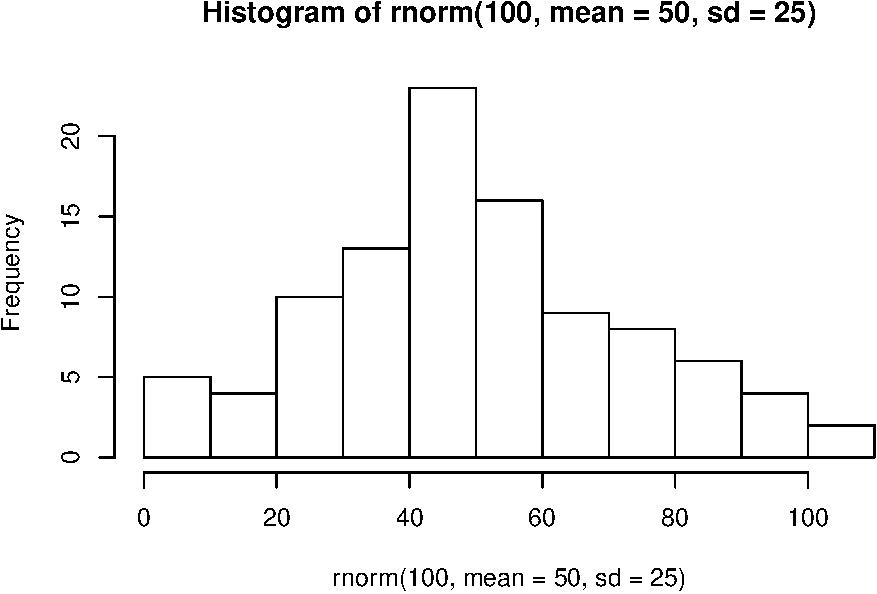
\includegraphics{Programming_Crump_files/figure-latex/unnamed-chunk-2-1.pdf}

You just made R sample 100 numbers, and then plot the results in a
histogram. Pretty neat. We'll be doing some of this later in the course,
where get R to make fake data for us, and then we learn to think about
how data behaves under different kinds of assumptions.

For now, let's do something that might be a little bit more
interesting\ldots{}what movies are going to be filming in NYC? It turns
out that NYC makes a lot of data about a lot things open and free for
anyone to download and look at. This is the NYC Open Data website:
\url{https://opendata.cityofnewyork.us}. I searched through the data,
and found this data file that lists the locations of film permits for
shooting movies all throughout the Burroughs. You can download the data
to your computer from
\href{https://raw.githubusercontent.com/CrumpLab/statisticsLab/master/data/Film_Permits.csv}{this
link}

NOTE TO SELF, COME BACK HERE AND WALKTHROUGH FILE PATHS AND THINGS

\begin{Shaded}
\begin{Highlighting}[]
\KeywordTok{library}\NormalTok{(data.table)}
\NormalTok{nyc_films <-}\KeywordTok{fread}\NormalTok{(}\StringTok{"data/Film_Permits.csv"}\NormalTok{)}
\end{Highlighting}
\end{Shaded}

\subsection{Look at the data}\label{look-at-the-data}

You will be downloading and analyzing all kinds of data files this
semester. We will follow the very same steps every time. The steps are
to load the data, then look at it. You want to see what you've got.

In R-studio, you will now see a variable called \texttt{nyc\_films} in
the top right-hand corner of the screen, in the environment tab. If you
click this thing, it will show you the contents of the data in a new
window. The data is stored in something we call a \texttt{data\ frame}.
It's R lingo, for the thing that contains the data. Notice is a square,
with rows going across, and columns going up and down. It looks kind of
like an excel spreadsheet if you are familiar with Excel.

It's useful to know you can look at the data frame this way if you need
to. But, this data frame is really big, it has 50,728 rows of data.
That's a lot too much to look at.

\subsubsection{summarytools}\label{summarytools}

The summarytools packages give a quick way to summarize all of the data
in a data frame. Here's how. When you run this code you will see the
summary in the viewer on the bottom right hand side. There's a little
browser button (arrow on top of little window) that you can click to
expand and see the whole thing in a browser.

\begin{Shaded}
\begin{Highlighting}[]
\KeywordTok{library}\NormalTok{(summarytools)}
\KeywordTok{view}\NormalTok{(}\KeywordTok{dfSummary}\NormalTok{(nyc_films))}
\end{Highlighting}
\end{Shaded}

That is super helpful, but it's still a lot to look at. Because there is
so much data here, it's pretty much mind-boggling to start thinking
about what to do with it.

\subsection{Make Plots to answer
questions}\label{make-plots-to-answer-questions}

Let's walk through a couple questions we might have about this data. We
can see that there were 50,728 film permits made. We can also see that
there are different columns telling us information about each of the
film permits. For example, the \texttt{Borough} column lists the Borough
for each request, whether it was made for: Manhattan, Brooklyn, Bronx,
Queen's, or Staten Island. Now we can ask our first question, and learn
how to do some plotting in R.

\subsubsection{Where are the most film permits being
requested?}\label{where-are-the-most-film-permits-being-requested}

Do you have any guesses? Is it Manhattan, or Brooklyn, of the Bronx? Or
Queen's or Staten Island? We can find out by plotting the data using a
bar plot. We just need to count how many film permits are made in each
borough, and then make different bars represent the the counts.

First, we do the counting in R. Run the following code.

\begin{Shaded}
\begin{Highlighting}[]
\KeywordTok{library}\NormalTok{(dplyr)}

\NormalTok{counts <-}\StringTok{ }\NormalTok{nyc_films %>%}
\StringTok{          }\KeywordTok{group_by}\NormalTok{(Borough) %>%}
\StringTok{          }\KeywordTok{summarize}\NormalTok{(}\DataTypeTok{count_of_permits =} \KeywordTok{length}\NormalTok{(Borough))}
\end{Highlighting}
\end{Shaded}

The above grouped the data by each of the five Borough's, and then
counted the number of times each Borough occurred (using the
\texttt{length} function). The result is a new variable called
\texttt{count}. I chose to name this variable \texttt{count}. You can
see that it is now displayed in the top-right hand corned in the
environment tab. If you gave \texttt{count} a different name, like
\texttt{muppets}, then it would be named what you called it.

If you click on the \texttt{counts} variable, you will see the five
boroughs listed, along with the counts for how many film permits were
requested in each Borough. These are the numbers that we want to plot in
a graph.

We do the plot using a fantastic package called \texttt{ggplot2}. It is
very powerful once you get the hand of it, and when you do, you will be
able to make all sorts of interesting graphs. Here's the code to make
the plot

\begin{Shaded}
\begin{Highlighting}[]
\KeywordTok{library}\NormalTok{(ggplot2)}

\KeywordTok{ggplot}\NormalTok{(counts, }\KeywordTok{aes}\NormalTok{(}\DataTypeTok{x =} \NormalTok{Borough, }\DataTypeTok{y =} \NormalTok{count_of_permits )) +}
\StringTok{  }\KeywordTok{geom_bar}\NormalTok{(}\DataTypeTok{stat=}\StringTok{"identity"}\NormalTok{)}
\end{Highlighting}
\end{Shaded}

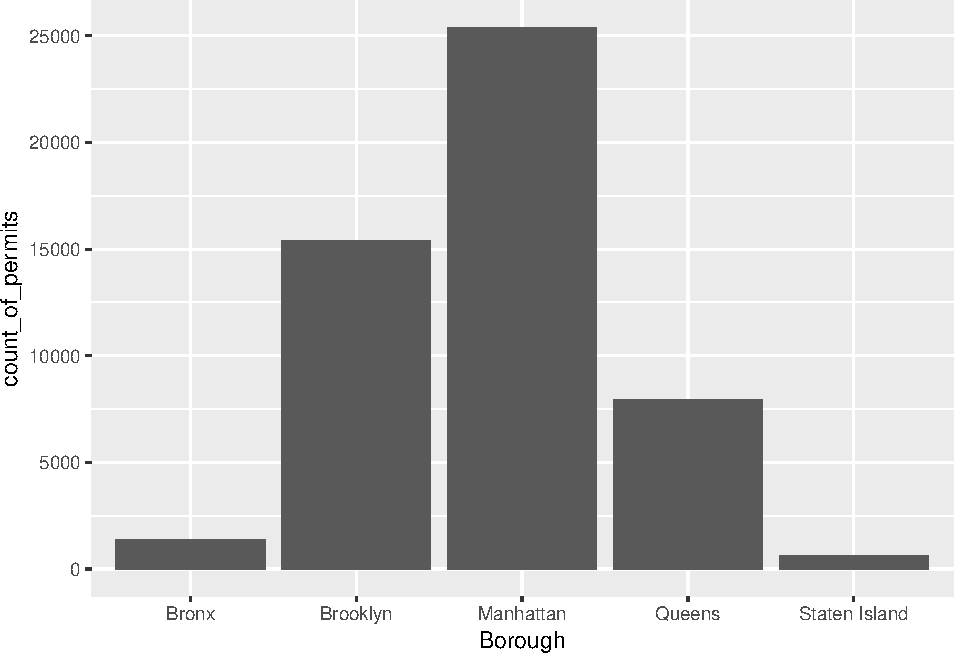
\includegraphics{Programming_Crump_files/figure-latex/unnamed-chunk-6-1.pdf}

There it is, we're done here! We can easily look at this graph, and
answer our question. Most of the film permits were requested in
Manhattan, followed by Brooklyn, then Queen's, the Bronx, and finally
Staten Island.

\subsubsection{\texorpdfstring{What kind of ``films'' are being made,
what is the
category?}{What kind of films are being made, what is the category?}}\label{what-kind-of-films-are-being-made-what-is-the-category}

We think you might be skeptical of what you are doing here, copying and
pasting things. Soon you'll see just how fast you can do things by
copying and pasting, and make a few little changes. Let's quickly ask
another question about what kinds of films are being made. The column
\texttt{Category}, gives us some information about that. Let's just copy
paste the code we already made, and see what kinds of categories the
films fall into. See if you can tell what I changed in the code to make
this work, I'll do it all at once:

\begin{Shaded}
\begin{Highlighting}[]
\NormalTok{counts <-}\StringTok{ }\NormalTok{nyc_films %>%}
\StringTok{          }\KeywordTok{group_by}\NormalTok{(Category) %>%}
\StringTok{          }\KeywordTok{summarize}\NormalTok{(}\DataTypeTok{count_of_permits =} \KeywordTok{length}\NormalTok{(Category))}

\KeywordTok{ggplot}\NormalTok{(counts, }\KeywordTok{aes}\NormalTok{(}\DataTypeTok{x =} \NormalTok{Category, }\DataTypeTok{y =} \NormalTok{count_of_permits )) +}
\StringTok{  }\KeywordTok{geom_bar}\NormalTok{(}\DataTypeTok{stat=}\StringTok{"identity"}\NormalTok{)+}\StringTok{ }
\StringTok{  }\KeywordTok{theme}\NormalTok{(}\DataTypeTok{axis.text.x =} \KeywordTok{element_text}\NormalTok{(}\DataTypeTok{angle =} \DecValTok{90}\NormalTok{, }\DataTypeTok{hjust =} \DecValTok{1}\NormalTok{))}
\end{Highlighting}
\end{Shaded}

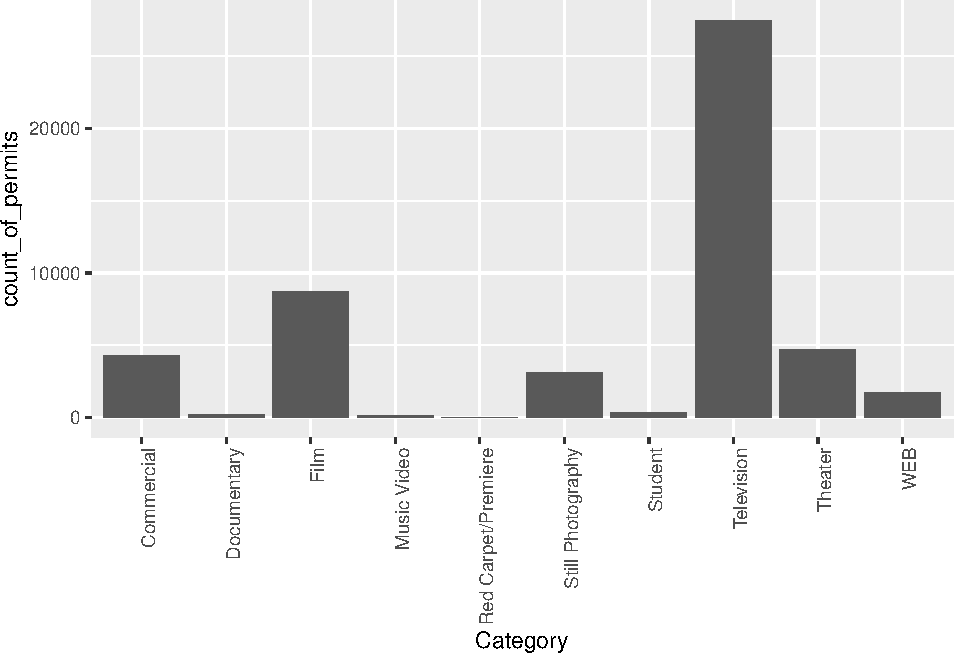
\includegraphics{Programming_Crump_files/figure-latex/unnamed-chunk-7-1.pdf}

OK, so this figure might look a bit weird because the labels on the
bottom are running into each other. We'll fix that in a bit. First,
let's notice the changes.

\begin{enumerate}
\def\labelenumi{\arabic{enumi}.}
\item
  I changed \texttt{Borough} to \texttt{Category}. That was the main
  thing
\item
  I left out a bunch of things from before. None of the
  \texttt{library()} commands are used again, and I didn't re-run the
  very early code to get the data. R already has those things in it's
  memory, so we don't need to do that first. If you ever clear the
  memory of R, then you will need to reload those things. First-things
  come first.
\end{enumerate}

Fine, so how do we fix the graph? Good question. To be honest, I don't
know right now. I totally forgot how. But, I know ggplot2 can do this,
and I'm going to Google it, right now. Then I'm going to find the
answer, and use it here. The googling of your questions is a fine way to
learn. It's what everybody does these days\ldots{}.{[}goes to
Google\ldots{}{]}.

Found it, actually found a lot of ways to do this. The trick is to add
the last line. I just copy-pasted it from the solution I found on
\href{https://stackoverflow.com/questions/1330989/rotating-and-spacing-axis-labels-in-ggplot2}{stack
overflow} (you will become friend's with stack overflow, there are many
solutions there to all of your questions)

\begin{Shaded}
\begin{Highlighting}[]
\NormalTok{counts <-}\StringTok{ }\NormalTok{nyc_films %>%}
\StringTok{          }\KeywordTok{group_by}\NormalTok{(Category) %>%}
\StringTok{          }\KeywordTok{summarize}\NormalTok{(}\DataTypeTok{count_of_permits =} \KeywordTok{length}\NormalTok{(Category))}

\KeywordTok{ggplot}\NormalTok{(counts, }\KeywordTok{aes}\NormalTok{(}\DataTypeTok{x =} \NormalTok{Category, }\DataTypeTok{y =} \NormalTok{count_of_permits )) +}
\StringTok{  }\KeywordTok{geom_bar}\NormalTok{(}\DataTypeTok{stat=}\StringTok{"identity"}\NormalTok{)+}\StringTok{ }
\StringTok{  }\KeywordTok{theme}\NormalTok{(}\DataTypeTok{axis.text.x =} \KeywordTok{element_text}\NormalTok{(}\DataTypeTok{angle =} \DecValTok{90}\NormalTok{, }\DataTypeTok{hjust =} \DecValTok{1}\NormalTok{))}
\end{Highlighting}
\end{Shaded}

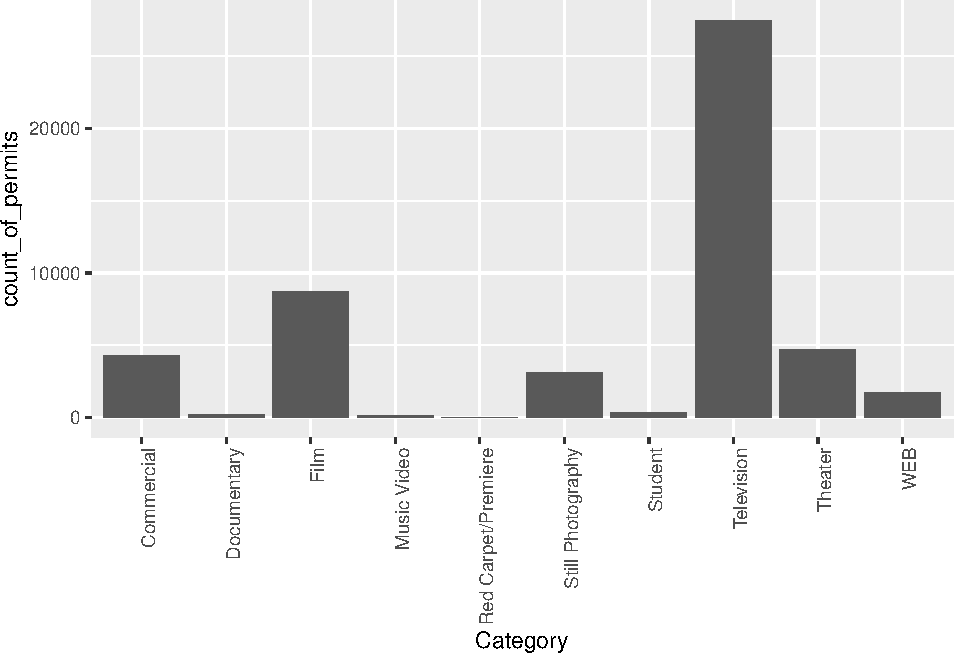
\includegraphics{Programming_Crump_files/figure-latex/unnamed-chunk-8-1.pdf}

\subsection{ggplot2 basics}\label{ggplot2-basics}

Before we go further, I want to point out some basic properties of
ggplot2, just to give you a sense of how it is working. This will make
more sense in a few weeks, so come back here to remind yourself. We'll
do just a bit a basics, and then move on to making more graphs, by
copying and pasting.

The ggplot function uses layers. Layers you say? What are these layers?
Well, it draws things from the bottom up. It lays down one layer of
graphics, then you can keep adding on top, drawing more things. So the
idea is something like: Layer 1 + Layer 2 + Layer 3, and so on. If you
want Layer 3 to be Layer 2, then you just switch them in the code.

Here is a way of thinking about ggplot code

\begin{verbatim}
ggplot(name_of_data, aes(x = name_of_x_variable, y = name_of_y_variable)) +
    geom_layer()+
    geom_layer()+
    geom_layer()
\end{verbatim}

What I want you to focus on in the above description is the \(+\) signs.
What we are doing with the plus signs is adding layers to plot. The
layers get added in the order that they are written. If you look back to
our previous code, you will see we add a \texttt{geom\_bar} layer, then
we added another layer to change the rotation of the words on the
x-axis. This is how it works.

BUT WAIT? How am I supposed to know what to add? This is nuts! We know.
You're not supposed to know just yet, how could you? We'll give you lots
of examples where you can copy and paste, and they will work. That's how
you'll learn. If you really want to read the
\href{https://ggplot2.tidyverse.org/reference/index.html}{help manual}
you can do that too. It's on the ggplot2 website. This will become
useful after you already know what you are doing, before that, it will
probably just seem very confusing. However, it is pretty neat to look
and \href{http://www.ggplot2-exts.org/gallery/}{see all of the different
things you can do}, it's very powerful.

For now, let's the get the hang of adding things to the graph that let
us change some stuff we might want to change. For example, how do you
add a title? Or change the labels on the axes? Or add different colors,
or change the font-size, or change the background? You can change all of
these things by adding different lines to the existing code.

\subsubsection{ylab() changes y label}\label{ylab-changes-y-label}

The last graph had \texttt{count\_of\_permits} as the label on the
y-axis. That doesn't look right. ggplot2 automatically took the label
from the column, and made it be the name on the y-axis. We can change
that by adding \texttt{ylab("what\ we\ want")}. We do this by adding a
\(+\) to the last line, then adding \texttt{ylab()}

\begin{Shaded}
\begin{Highlighting}[]
\KeywordTok{ggplot}\NormalTok{(counts, }\KeywordTok{aes}\NormalTok{(}\DataTypeTok{x =} \NormalTok{Category, }\DataTypeTok{y =} \NormalTok{count_of_permits )) +}
\StringTok{  }\KeywordTok{geom_bar}\NormalTok{(}\DataTypeTok{stat=}\StringTok{"identity"}\NormalTok{) +}\StringTok{ }
\StringTok{  }\KeywordTok{theme}\NormalTok{(}\DataTypeTok{axis.text.x =} \KeywordTok{element_text}\NormalTok{(}\DataTypeTok{angle =} \DecValTok{90}\NormalTok{, }\DataTypeTok{hjust =} \DecValTok{1}\NormalTok{)) +}
\StringTok{  }\KeywordTok{ylab}\NormalTok{(}\StringTok{"Number of Film Permits"}\NormalTok{)}
\end{Highlighting}
\end{Shaded}

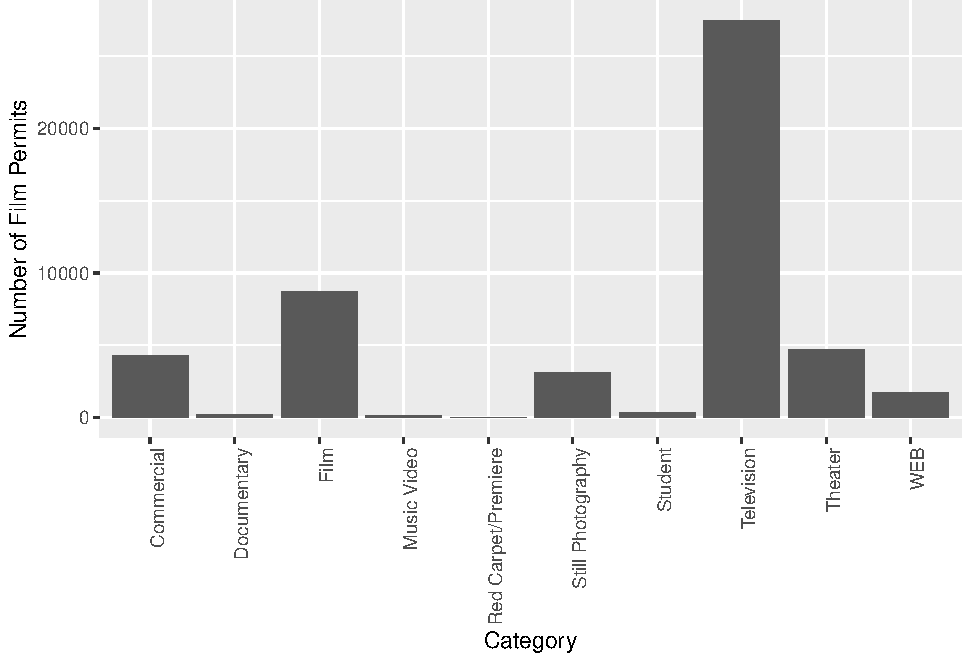
\includegraphics{Programming_Crump_files/figure-latex/unnamed-chunk-9-1.pdf}

\subsubsection{xlab() changes x label}\label{xlab-changes-x-label}

Let's slightly modify the x label too:

\begin{Shaded}
\begin{Highlighting}[]
\KeywordTok{ggplot}\NormalTok{(counts, }\KeywordTok{aes}\NormalTok{(}\DataTypeTok{x =} \NormalTok{Category, }\DataTypeTok{y =} \NormalTok{count_of_permits )) +}
\StringTok{  }\KeywordTok{geom_bar}\NormalTok{(}\DataTypeTok{stat=}\StringTok{"identity"}\NormalTok{) +}\StringTok{ }
\StringTok{  }\KeywordTok{theme}\NormalTok{(}\DataTypeTok{axis.text.x =} \KeywordTok{element_text}\NormalTok{(}\DataTypeTok{angle =} \DecValTok{90}\NormalTok{, }\DataTypeTok{hjust =} \DecValTok{1}\NormalTok{)) +}
\StringTok{  }\KeywordTok{ylab}\NormalTok{(}\StringTok{"Number of Film Permits"}\NormalTok{) +}\StringTok{ }
\StringTok{  }\KeywordTok{xlab}\NormalTok{(}\StringTok{"Category of film"}\NormalTok{)}
\end{Highlighting}
\end{Shaded}

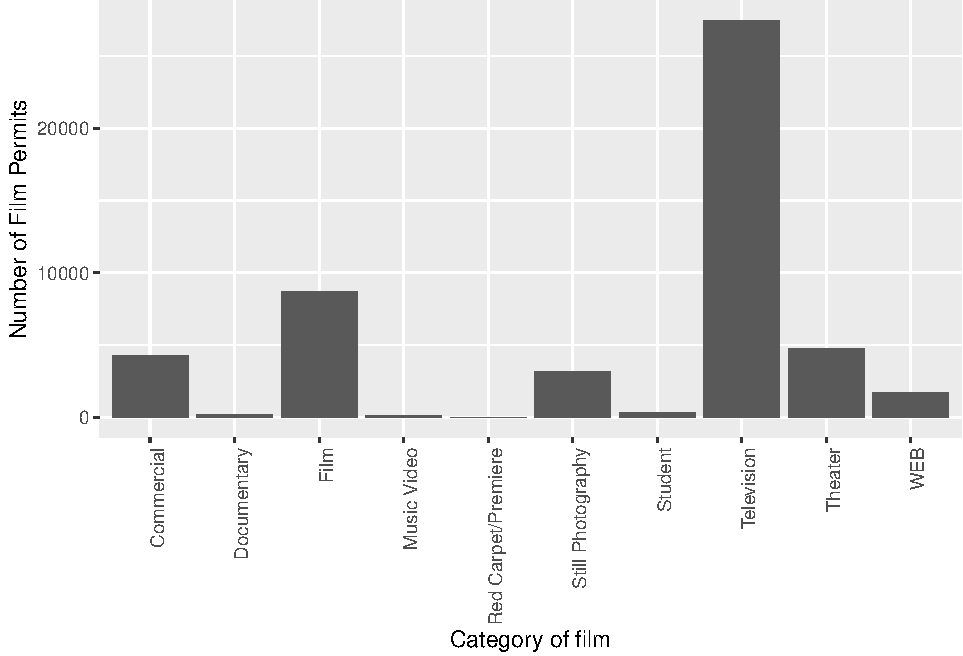
\includegraphics{Programming_Crump_files/figure-latex/unnamed-chunk-10-1.pdf}

\subsubsection{ggtitle() adds title}\label{ggtitle-adds-title}

Let's give our graph a title

\begin{Shaded}
\begin{Highlighting}[]
\KeywordTok{ggplot}\NormalTok{(counts, }\KeywordTok{aes}\NormalTok{(}\DataTypeTok{x =} \NormalTok{Category, }\DataTypeTok{y =} \NormalTok{count_of_permits )) +}
\StringTok{  }\KeywordTok{geom_bar}\NormalTok{(}\DataTypeTok{stat=}\StringTok{"identity"}\NormalTok{) +}\StringTok{ }
\StringTok{  }\KeywordTok{theme}\NormalTok{(}\DataTypeTok{axis.text.x =} \KeywordTok{element_text}\NormalTok{(}\DataTypeTok{angle =} \DecValTok{90}\NormalTok{, }\DataTypeTok{hjust =} \DecValTok{1}\NormalTok{)) +}
\StringTok{  }\KeywordTok{ylab}\NormalTok{(}\StringTok{"Number of Film Permits"}\NormalTok{) +}\StringTok{ }
\StringTok{  }\KeywordTok{xlab}\NormalTok{(}\StringTok{"Category of film"}\NormalTok{) +}
\StringTok{  }\KeywordTok{ggtitle}\NormalTok{(}\StringTok{"Number of Film permits in NYC by Category"}\NormalTok{)}
\end{Highlighting}
\end{Shaded}

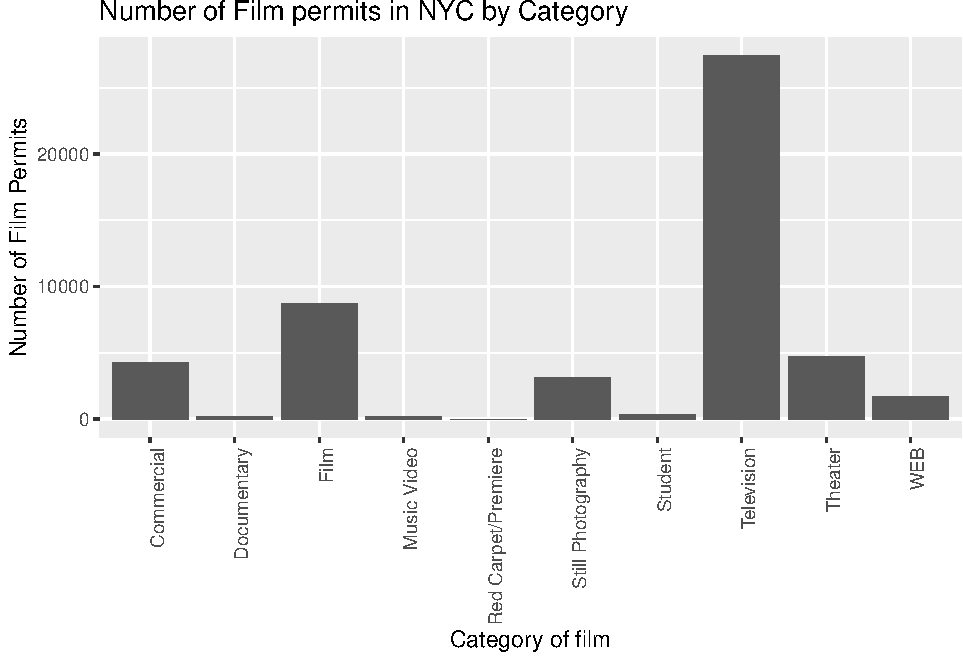
\includegraphics{Programming_Crump_files/figure-latex/unnamed-chunk-11-1.pdf}

\subsubsection{color adds color}\label{color-adds-color}

Let's make the bars different colors. To do this, we add new code to the
inside of the \texttt{aes()} part:

\begin{Shaded}
\begin{Highlighting}[]
\KeywordTok{ggplot}\NormalTok{(counts, }\KeywordTok{aes}\NormalTok{(}\DataTypeTok{x =} \NormalTok{Category, }\DataTypeTok{y =} \NormalTok{count_of_permits, }\DataTypeTok{color=}\NormalTok{Category )) +}
\StringTok{  }\KeywordTok{geom_bar}\NormalTok{(}\DataTypeTok{stat=}\StringTok{"identity"}\NormalTok{) +}\StringTok{ }
\StringTok{  }\KeywordTok{theme}\NormalTok{(}\DataTypeTok{axis.text.x =} \KeywordTok{element_text}\NormalTok{(}\DataTypeTok{angle =} \DecValTok{90}\NormalTok{, }\DataTypeTok{hjust =} \DecValTok{1}\NormalTok{)) +}
\StringTok{  }\KeywordTok{ylab}\NormalTok{(}\StringTok{"Number of Film Permits"}\NormalTok{) +}\StringTok{ }
\StringTok{  }\KeywordTok{xlab}\NormalTok{(}\StringTok{"Category of film"}\NormalTok{) +}
\StringTok{  }\KeywordTok{ggtitle}\NormalTok{(}\StringTok{"Number of Film permits in NYC by Category"}\NormalTok{)}
\end{Highlighting}
\end{Shaded}

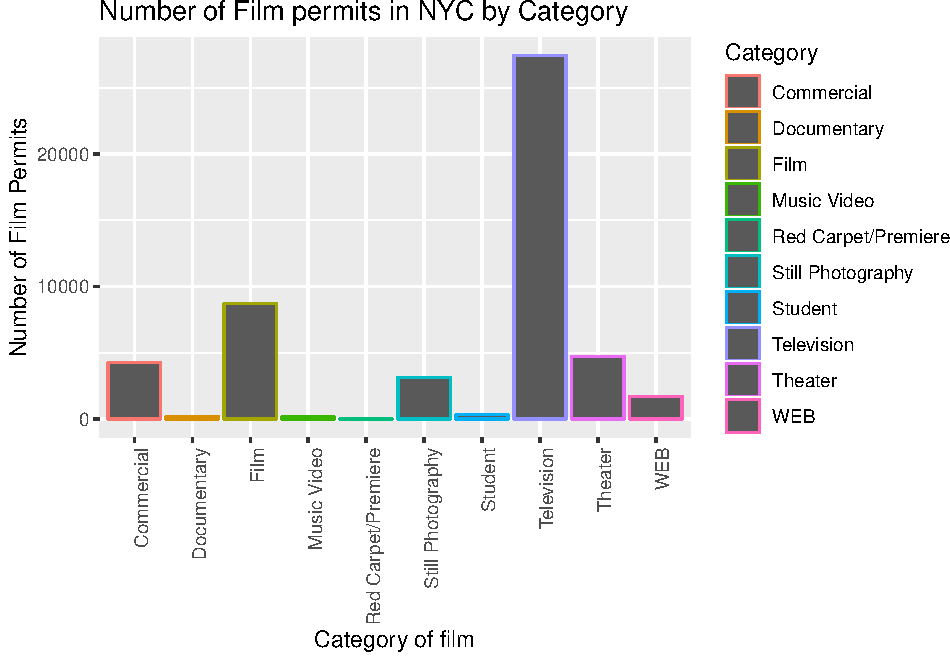
\includegraphics{Programming_Crump_files/figure-latex/unnamed-chunk-12-1.pdf}

\subsubsection{fill fills in color}\label{fill-fills-in-color}

Let's make the bars different colors. To do this, we add new code to the
inside of the \texttt{aes()} part\ldots{}Notice I've started using new
lines to make the code more readable.

\begin{Shaded}
\begin{Highlighting}[]
\KeywordTok{ggplot}\NormalTok{(counts, }\KeywordTok{aes}\NormalTok{(}\DataTypeTok{x =} \NormalTok{Category, }\DataTypeTok{y =} \NormalTok{count_of_permits, }
                   \DataTypeTok{color=}\NormalTok{Category, }
                   \DataTypeTok{fill=} \NormalTok{Category )) +}
\StringTok{  }\KeywordTok{geom_bar}\NormalTok{(}\DataTypeTok{stat=}\StringTok{"identity"}\NormalTok{) +}\StringTok{ }
\StringTok{  }\KeywordTok{theme}\NormalTok{(}\DataTypeTok{axis.text.x =} \KeywordTok{element_text}\NormalTok{(}\DataTypeTok{angle =} \DecValTok{90}\NormalTok{, }\DataTypeTok{hjust =} \DecValTok{1}\NormalTok{)) +}
\StringTok{  }\KeywordTok{ylab}\NormalTok{(}\StringTok{"Number of Film Permits"}\NormalTok{) +}\StringTok{ }
\StringTok{  }\KeywordTok{xlab}\NormalTok{(}\StringTok{"Category of film"}\NormalTok{) +}
\StringTok{  }\KeywordTok{ggtitle}\NormalTok{(}\StringTok{"Number of Film permits in NYC by Category"}\NormalTok{)}
\end{Highlighting}
\end{Shaded}

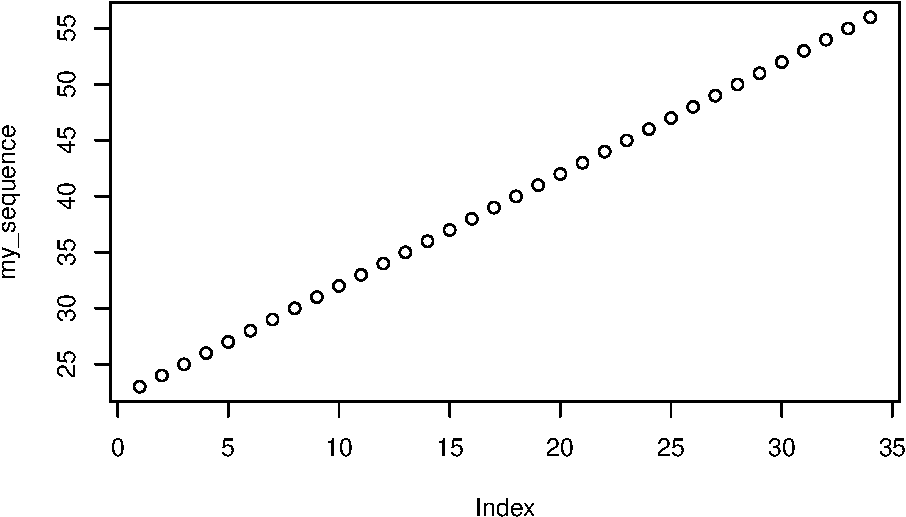
\includegraphics{Programming_Crump_files/figure-latex/unnamed-chunk-13-1.pdf}

\subsubsection{get rid of the legend}\label{get-rid-of-the-legend}

Sometimes you just don't want the legend on the side, to remove it add

\texttt{theme(legend.position="none")}

\begin{Shaded}
\begin{Highlighting}[]
\KeywordTok{ggplot}\NormalTok{(counts, }\KeywordTok{aes}\NormalTok{(}\DataTypeTok{x =} \NormalTok{Category, }\DataTypeTok{y =} \NormalTok{count_of_permits, }
                   \DataTypeTok{color=}\NormalTok{Category, }
                   \DataTypeTok{fill=} \NormalTok{Category )) +}
\StringTok{  }\KeywordTok{geom_bar}\NormalTok{(}\DataTypeTok{stat=}\StringTok{"identity"}\NormalTok{) +}\StringTok{ }
\StringTok{  }\KeywordTok{theme}\NormalTok{(}\DataTypeTok{axis.text.x =} \KeywordTok{element_text}\NormalTok{(}\DataTypeTok{angle =} \DecValTok{90}\NormalTok{, }\DataTypeTok{hjust =} \DecValTok{1}\NormalTok{)) +}
\StringTok{  }\KeywordTok{ylab}\NormalTok{(}\StringTok{"Number of Film Permits"}\NormalTok{) +}\StringTok{ }
\StringTok{  }\KeywordTok{xlab}\NormalTok{(}\StringTok{"Category of film"}\NormalTok{) +}
\StringTok{  }\KeywordTok{ggtitle}\NormalTok{(}\StringTok{"Number of Film permits in NYC by Category"}\NormalTok{) +}
\StringTok{  }\KeywordTok{theme}\NormalTok{(}\DataTypeTok{legend.position=}\StringTok{"none"}\NormalTok{)}
\end{Highlighting}
\end{Shaded}

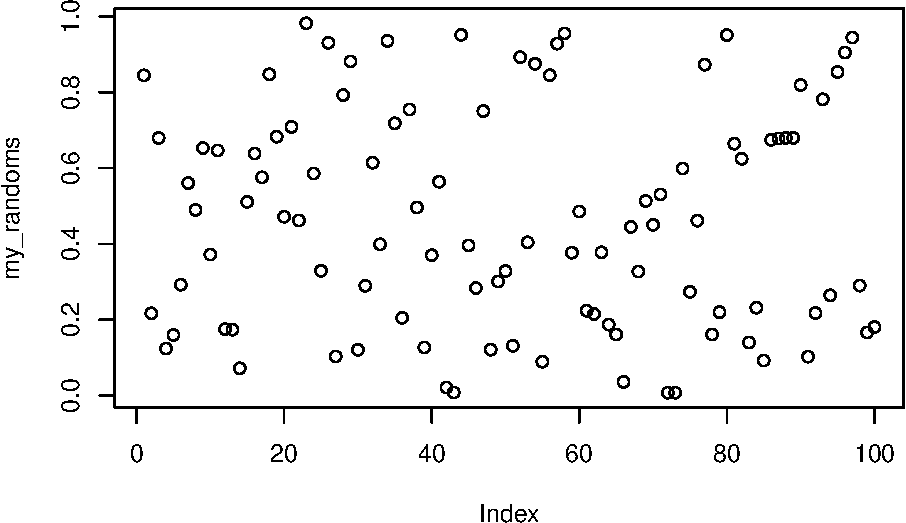
\includegraphics{Programming_Crump_files/figure-latex/unnamed-chunk-14-1.pdf}

\subsubsection{theme\_classic() makes white
background}\label{theme_classic-makes-white-background}

The rest is often just visual preference. For example, the graph above
has this grey grid behind the bars. For a clean classic no nonsense
look, use \texttt{theme\_classic()} to take away the grid.

\begin{Shaded}
\begin{Highlighting}[]
\KeywordTok{ggplot}\NormalTok{(counts, }\KeywordTok{aes}\NormalTok{(}\DataTypeTok{x =} \NormalTok{Category, }\DataTypeTok{y =} \NormalTok{count_of_permits, }
                   \DataTypeTok{color=}\NormalTok{Category, }
                   \DataTypeTok{fill=} \NormalTok{Category )) +}
\StringTok{  }\KeywordTok{geom_bar}\NormalTok{(}\DataTypeTok{stat=}\StringTok{"identity"}\NormalTok{) +}\StringTok{ }
\StringTok{  }\KeywordTok{theme}\NormalTok{(}\DataTypeTok{axis.text.x =} \KeywordTok{element_text}\NormalTok{(}\DataTypeTok{angle =} \DecValTok{90}\NormalTok{, }\DataTypeTok{hjust =} \DecValTok{1}\NormalTok{)) +}
\StringTok{  }\KeywordTok{ylab}\NormalTok{(}\StringTok{"Number of Film Permits"}\NormalTok{) +}\StringTok{ }
\StringTok{  }\KeywordTok{xlab}\NormalTok{(}\StringTok{"Category of film"}\NormalTok{) +}
\StringTok{  }\KeywordTok{ggtitle}\NormalTok{(}\StringTok{"Number of Film permits in NYC by Category"}\NormalTok{) +}
\StringTok{  }\KeywordTok{theme}\NormalTok{(}\DataTypeTok{legend.position=}\StringTok{"none"}\NormalTok{) +}
\StringTok{  }\KeywordTok{theme_classic}\NormalTok{()}
\end{Highlighting}
\end{Shaded}

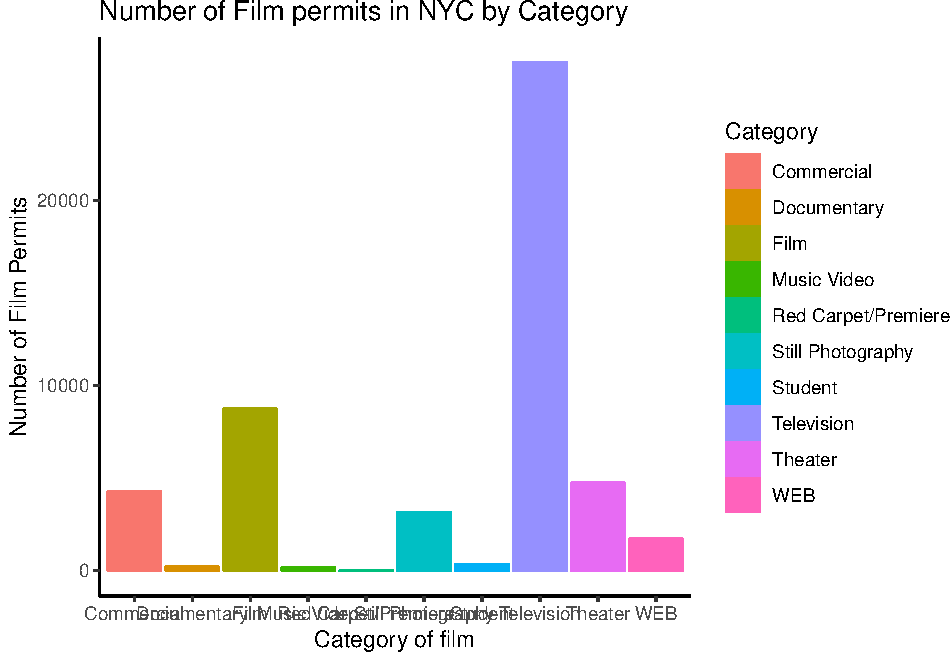
\includegraphics{Programming_Crump_files/figure-latex/unnamed-chunk-15-1.pdf}

\subsubsection{Sometimes layer order
matters}\label{sometimes-layer-order-matters}

Interesting, \texttt{theme\_classic()} is misbehaving a little bit. It
looks like we have some of our layer out of order, let's re-order. I
just moved \texttt{theme\_classic()} to just underneath the
\texttt{geom\_bar()} line. Now everything get's drawn properly.

\begin{Shaded}
\begin{Highlighting}[]
\KeywordTok{ggplot}\NormalTok{(counts, }\KeywordTok{aes}\NormalTok{(}\DataTypeTok{x =} \NormalTok{Category, }\DataTypeTok{y =} \NormalTok{count_of_permits, }
                   \DataTypeTok{color=}\NormalTok{Category, }
                   \DataTypeTok{fill=} \NormalTok{Category )) +}
\StringTok{  }\KeywordTok{geom_bar}\NormalTok{(}\DataTypeTok{stat=}\StringTok{"identity"}\NormalTok{) +}\StringTok{ }
\StringTok{  }\KeywordTok{theme_classic}\NormalTok{() +}
\StringTok{  }\KeywordTok{theme}\NormalTok{(}\DataTypeTok{axis.text.x =} \KeywordTok{element_text}\NormalTok{(}\DataTypeTok{angle =} \DecValTok{90}\NormalTok{, }\DataTypeTok{hjust =} \DecValTok{1}\NormalTok{)) +}
\StringTok{  }\KeywordTok{ylab}\NormalTok{(}\StringTok{"Number of Film Permits"}\NormalTok{) +}\StringTok{ }
\StringTok{  }\KeywordTok{xlab}\NormalTok{(}\StringTok{"Category of film"}\NormalTok{) +}
\StringTok{  }\KeywordTok{ggtitle}\NormalTok{(}\StringTok{"Number of Film permits in NYC by Category"}\NormalTok{) +}
\StringTok{  }\KeywordTok{theme}\NormalTok{(}\DataTypeTok{legend.position=}\StringTok{"none"}\NormalTok{) }
\end{Highlighting}
\end{Shaded}

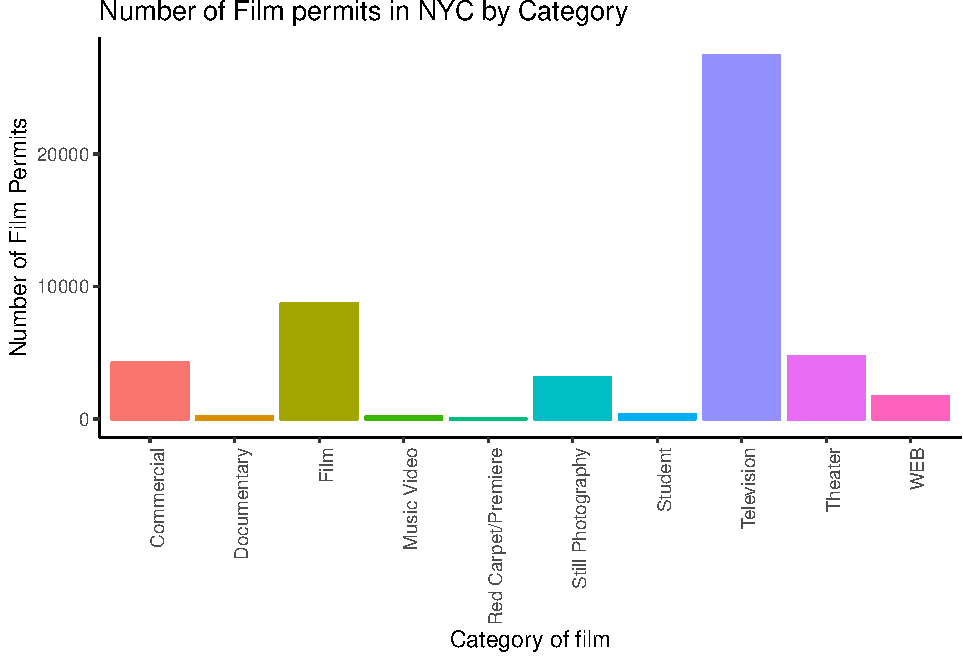
\includegraphics{Programming_Crump_files/figure-latex/unnamed-chunk-16-1.pdf}

\subsubsection{Font-size}\label{font-size}

Changing font-size is often something you want to do. ggplot2 can do
this in different ways. I suggest using the \texttt{base\_size} option
inside \texttt{theme\_classic()}. You set one number for the largest
font size in the graph, and everything else gets scaled to fit with that
that first number. It's really convenient. Look for the inside of
\texttt{theme\_classic()}

\begin{Shaded}
\begin{Highlighting}[]
\KeywordTok{ggplot}\NormalTok{(counts, }\KeywordTok{aes}\NormalTok{(}\DataTypeTok{x =} \NormalTok{Category, }\DataTypeTok{y =} \NormalTok{count_of_permits, }
                   \DataTypeTok{color=}\NormalTok{Category, }
                   \DataTypeTok{fill=} \NormalTok{Category )) +}
\StringTok{  }\KeywordTok{geom_bar}\NormalTok{(}\DataTypeTok{stat=}\StringTok{"identity"}\NormalTok{) +}\StringTok{ }
\StringTok{  }\KeywordTok{theme_classic}\NormalTok{(}\DataTypeTok{base_size =} \DecValTok{15}\NormalTok{) +}
\StringTok{  }\KeywordTok{theme}\NormalTok{(}\DataTypeTok{axis.text.x =} \KeywordTok{element_text}\NormalTok{(}\DataTypeTok{angle =} \DecValTok{90}\NormalTok{, }\DataTypeTok{hjust =} \DecValTok{1}\NormalTok{)) +}
\StringTok{  }\KeywordTok{ylab}\NormalTok{(}\StringTok{"Number of Film Permits"}\NormalTok{) +}\StringTok{ }
\StringTok{  }\KeywordTok{xlab}\NormalTok{(}\StringTok{"Category of film"}\NormalTok{) +}
\StringTok{  }\KeywordTok{ggtitle}\NormalTok{(}\StringTok{"Number of Film permits in NYC by Category"}\NormalTok{) +}
\StringTok{  }\KeywordTok{theme}\NormalTok{(}\DataTypeTok{legend.position=}\StringTok{"none"}\NormalTok{) }
\end{Highlighting}
\end{Shaded}

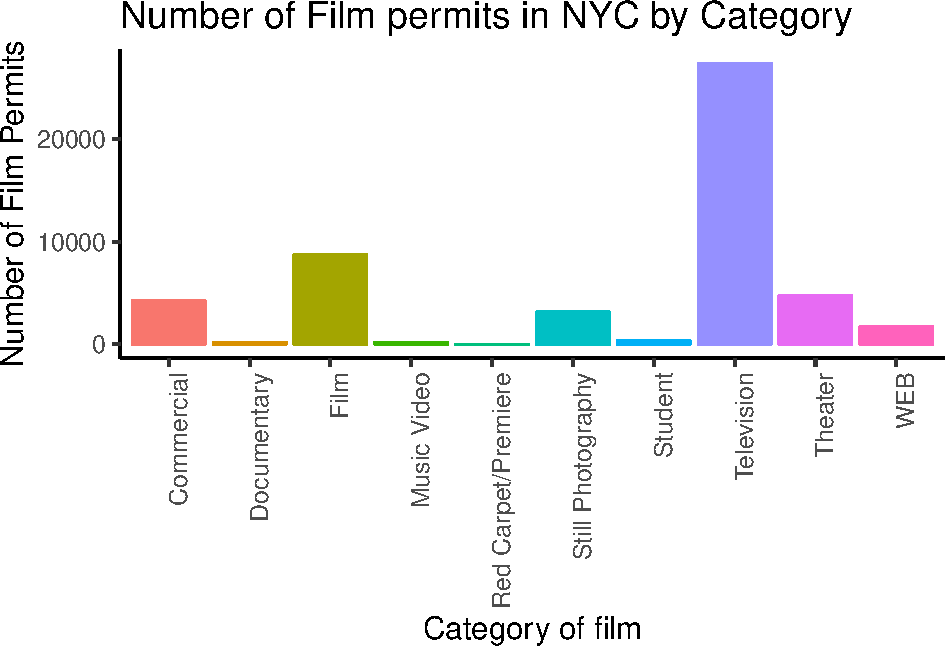
\includegraphics{Programming_Crump_files/figure-latex/unnamed-chunk-17-1.pdf}
or make things small\ldots{} just to see what happens

\begin{Shaded}
\begin{Highlighting}[]
\KeywordTok{ggplot}\NormalTok{(counts, }\KeywordTok{aes}\NormalTok{(}\DataTypeTok{x =} \NormalTok{Category, }\DataTypeTok{y =} \NormalTok{count_of_permits, }
                   \DataTypeTok{color=}\NormalTok{Category, }
                   \DataTypeTok{fill=} \NormalTok{Category )) +}
\StringTok{  }\KeywordTok{geom_bar}\NormalTok{(}\DataTypeTok{stat=}\StringTok{"identity"}\NormalTok{) +}\StringTok{ }
\StringTok{  }\KeywordTok{theme_classic}\NormalTok{(}\DataTypeTok{base_size =} \DecValTok{10}\NormalTok{) +}
\StringTok{  }\KeywordTok{theme}\NormalTok{(}\DataTypeTok{axis.text.x =} \KeywordTok{element_text}\NormalTok{(}\DataTypeTok{angle =} \DecValTok{90}\NormalTok{, }\DataTypeTok{hjust =} \DecValTok{1}\NormalTok{)) +}
\StringTok{  }\KeywordTok{ylab}\NormalTok{(}\StringTok{"Number of Film Permits"}\NormalTok{) +}\StringTok{ }
\StringTok{  }\KeywordTok{xlab}\NormalTok{(}\StringTok{"Category of film"}\NormalTok{) +}
\StringTok{  }\KeywordTok{ggtitle}\NormalTok{(}\StringTok{"Number of Film permits in NYC by Category"}\NormalTok{) +}
\StringTok{  }\KeywordTok{theme}\NormalTok{(}\DataTypeTok{legend.position=}\StringTok{"none"}\NormalTok{) }
\end{Highlighting}
\end{Shaded}

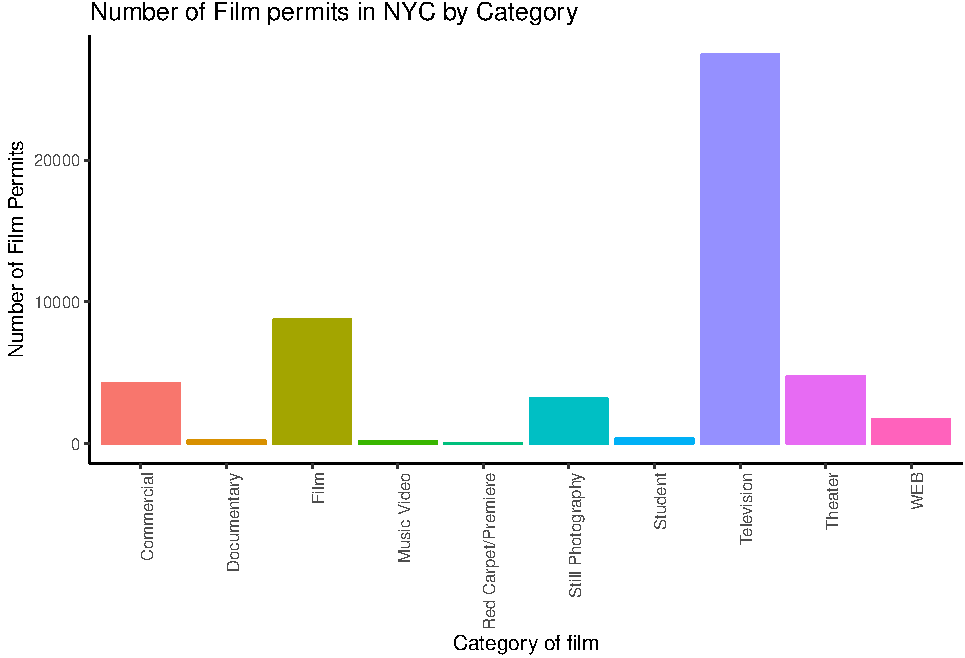
\includegraphics{Programming_Crump_files/figure-latex/unnamed-chunk-18-1.pdf}

\subsubsection{ggplot2 summary}\label{ggplot2-summary}

That's enough of the ggplot2 basics for now. You will discover that many
things are possible with ggplot2. It is amazing. We are going to get
back to answering some questions about the data with graphs. But, now
that we have built the code to make the graphs, all we need to do is
copy-paste, and make a few small changes, and boom, we have our graph.

\subsection{More questions about NYC
films}\label{more-questions-about-nyc-films}

\subsubsection{What are the sub-categories of
films?}\label{what-are-the-sub-categories-of-films}

Notice the \texttt{nyc\_films} data frame also has a column for
\texttt{SubCategoryName}. Let's see what's going on there with a quick
plot.

\begin{Shaded}
\begin{Highlighting}[]
\CommentTok{# get the counts (this is a comment it's just here for you to read)}

\NormalTok{counts <-}\StringTok{ }\NormalTok{nyc_films %>%}
\StringTok{          }\KeywordTok{group_by}\NormalTok{(SubCategoryName) %>%}
\StringTok{          }\KeywordTok{summarize}\NormalTok{(}\DataTypeTok{count_of_permits =} \KeywordTok{length}\NormalTok{(SubCategoryName))}

\CommentTok{# make the plot}

\KeywordTok{ggplot}\NormalTok{(counts, }\KeywordTok{aes}\NormalTok{(}\DataTypeTok{x =} \NormalTok{SubCategoryName, }\DataTypeTok{y =} \NormalTok{count_of_permits, }
                   \DataTypeTok{color=}\NormalTok{SubCategoryName, }
                   \DataTypeTok{fill=} \NormalTok{SubCategoryName )) +}
\StringTok{  }\KeywordTok{geom_bar}\NormalTok{(}\DataTypeTok{stat=}\StringTok{"identity"}\NormalTok{) +}\StringTok{ }
\StringTok{  }\KeywordTok{theme_classic}\NormalTok{(}\DataTypeTok{base_size =} \DecValTok{10}\NormalTok{) +}
\StringTok{  }\KeywordTok{theme}\NormalTok{(}\DataTypeTok{axis.text.x =} \KeywordTok{element_text}\NormalTok{(}\DataTypeTok{angle =} \DecValTok{90}\NormalTok{, }\DataTypeTok{hjust =} \DecValTok{1}\NormalTok{)) +}
\StringTok{  }\KeywordTok{ylab}\NormalTok{(}\StringTok{"Number of Film Permits"}\NormalTok{) +}\StringTok{ }
\StringTok{  }\KeywordTok{xlab}\NormalTok{(}\StringTok{"Sub-category of film"}\NormalTok{) +}
\StringTok{  }\KeywordTok{ggtitle}\NormalTok{(}\StringTok{"Number of Film permits in NYC by Sub-category"}\NormalTok{) +}
\StringTok{  }\KeywordTok{theme}\NormalTok{(}\DataTypeTok{legend.position=}\StringTok{"none"}\NormalTok{) }
\end{Highlighting}
\end{Shaded}

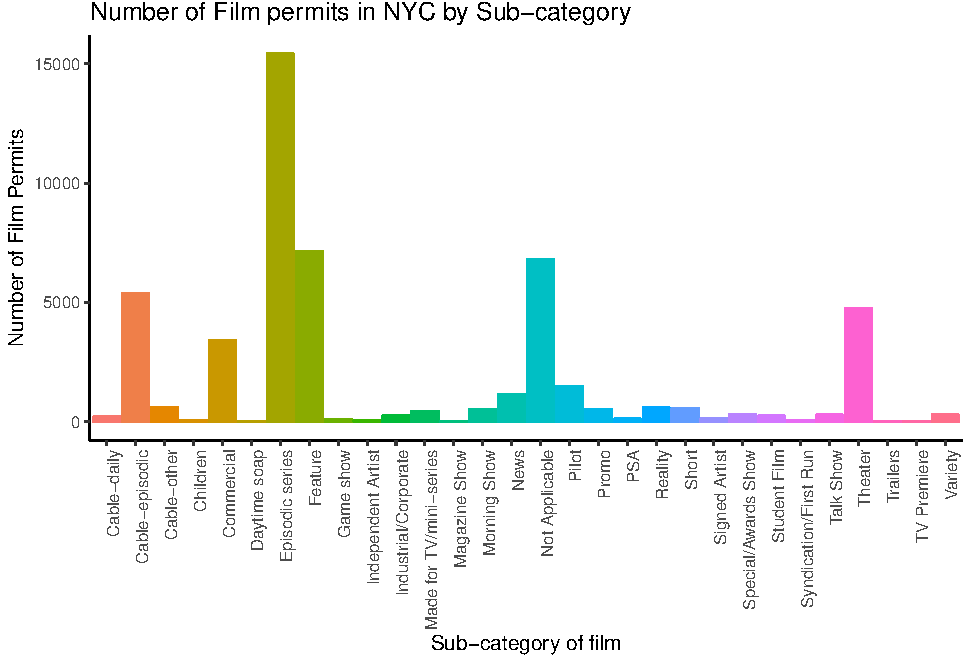
\includegraphics{Programming_Crump_files/figure-latex/unnamed-chunk-19-1.pdf}

I guess ``episodic series'' are the most common. Using a graph like this
gave us our answer super fast.

\subsubsection{Categories by different
Boroughs}\label{categories-by-different-boroughs}

Let's see one more really useful thing about ggplot2. It's called
\texttt{facet\_wrap()}. It's an ugly word, but you will see that it is
very cool, and you can do next-level-super-hero graph styles with
\texttt{facet\_wrap} that other people can't do very easily.

Here's our question. We know that some films are made in different
Boroughs, and that same films are made in different categories, but do
different Boroughs have different patterns for the kinds of categories
of films they request permits for? Are their more TV shows in Brooklyn?
How do we find out? Watch, just like this:

\begin{Shaded}
\begin{Highlighting}[]
\CommentTok{# get the counts (this is a comment it's just here for you to read)}

\NormalTok{counts <-}\StringTok{ }\NormalTok{nyc_films %>%}
\StringTok{          }\KeywordTok{group_by}\NormalTok{(Borough,Category) %>%}
\StringTok{          }\KeywordTok{summarize}\NormalTok{(}\DataTypeTok{count_of_permits =} \KeywordTok{length}\NormalTok{(Category))}

\CommentTok{# make the plot}

\KeywordTok{ggplot}\NormalTok{(counts, }\KeywordTok{aes}\NormalTok{(}\DataTypeTok{x =} \NormalTok{Category, }\DataTypeTok{y =} \NormalTok{count_of_permits, }
                   \DataTypeTok{color=}\NormalTok{Category, }
                   \DataTypeTok{fill=} \NormalTok{Category )) +}
\StringTok{  }\KeywordTok{geom_bar}\NormalTok{(}\DataTypeTok{stat=}\StringTok{"identity"}\NormalTok{) +}\StringTok{ }
\StringTok{  }\KeywordTok{theme_classic}\NormalTok{(}\DataTypeTok{base_size =} \DecValTok{10}\NormalTok{) +}
\StringTok{  }\KeywordTok{theme}\NormalTok{(}\DataTypeTok{axis.text.x =} \KeywordTok{element_text}\NormalTok{(}\DataTypeTok{angle =} \DecValTok{90}\NormalTok{, }\DataTypeTok{hjust =} \DecValTok{1}\NormalTok{)) +}
\StringTok{  }\KeywordTok{ylab}\NormalTok{(}\StringTok{"Number of Film Permits"}\NormalTok{) +}\StringTok{ }
\StringTok{  }\KeywordTok{xlab}\NormalTok{(}\StringTok{"Category of film"}\NormalTok{) +}
\StringTok{  }\KeywordTok{ggtitle}\NormalTok{(}\StringTok{"Number of Film permits in NYC by Category and Borough"}\NormalTok{) +}
\StringTok{  }\KeywordTok{theme}\NormalTok{(}\DataTypeTok{legend.position=}\StringTok{"none"}\NormalTok{) +}
\StringTok{  }\KeywordTok{facet_wrap}\NormalTok{(~Borough, }\DataTypeTok{ncol=}\DecValTok{3}\NormalTok{)}
\end{Highlighting}
\end{Shaded}

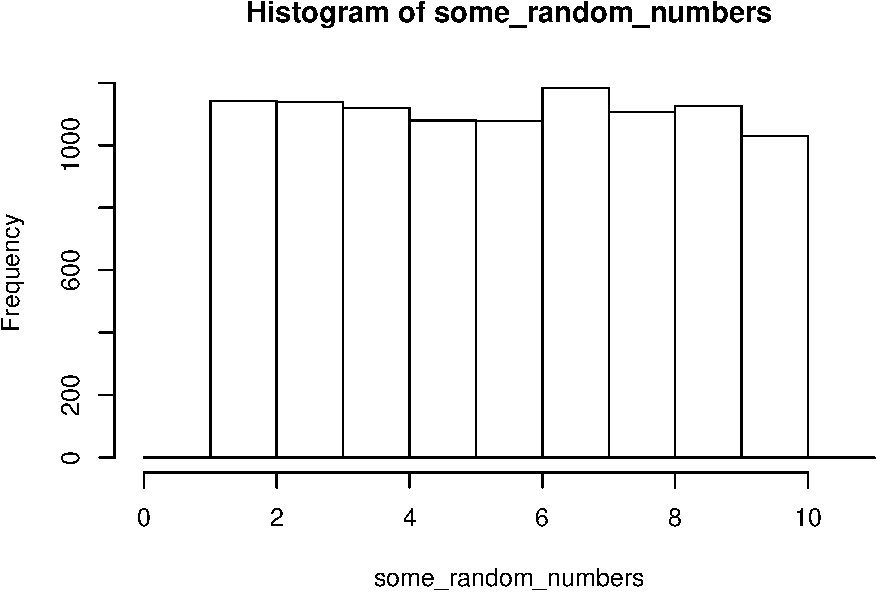
\includegraphics{Programming_Crump_files/figure-latex/unnamed-chunk-20-1.pdf}

We did two important things. First we added \texttt{Borough} and
\texttt{Category} into the \texttt{group\_by()} function. This
automatically gives separate counts for each category of film, for each
Borough. Then we added
\texttt{facet\_wrap(\textasciitilde{}Borough,\ ncol=3)} to the end of
the plot, and it automatically drew us 5 different bar graphs, one for
each Borough! That was fast. Imagine doing that by hand.

The nice thing about this is we can switch things around if we want. For
example, we could do it this way by switching the \texttt{Category} with
\texttt{Borough}, and facet-wrapping by Category instead of Borough like
we did above. Do what works for you.

\begin{Shaded}
\begin{Highlighting}[]
\KeywordTok{ggplot}\NormalTok{(counts, }\KeywordTok{aes}\NormalTok{(}\DataTypeTok{x =} \NormalTok{Borough, }\DataTypeTok{y =} \NormalTok{count_of_permits, }
                   \DataTypeTok{color=}\NormalTok{Borough, }
                   \DataTypeTok{fill=} \NormalTok{Borough )) +}
\StringTok{  }\KeywordTok{geom_bar}\NormalTok{(}\DataTypeTok{stat=}\StringTok{"identity"}\NormalTok{) +}\StringTok{ }
\StringTok{  }\KeywordTok{theme_classic}\NormalTok{(}\DataTypeTok{base_size =} \DecValTok{10}\NormalTok{) +}
\StringTok{  }\KeywordTok{theme}\NormalTok{(}\DataTypeTok{axis.text.x =} \KeywordTok{element_text}\NormalTok{(}\DataTypeTok{angle =} \DecValTok{90}\NormalTok{, }\DataTypeTok{hjust =} \DecValTok{1}\NormalTok{)) +}
\StringTok{  }\KeywordTok{ylab}\NormalTok{(}\StringTok{"Number of Film Permits"}\NormalTok{) +}\StringTok{ }
\StringTok{  }\KeywordTok{xlab}\NormalTok{(}\StringTok{"Borough"}\NormalTok{) +}
\StringTok{  }\KeywordTok{ggtitle}\NormalTok{(}\StringTok{"Number of Film permits in NYC by Category and Borough"}\NormalTok{) +}
\StringTok{  }\KeywordTok{theme}\NormalTok{(}\DataTypeTok{legend.position=}\StringTok{"none"}\NormalTok{) +}
\StringTok{  }\KeywordTok{facet_wrap}\NormalTok{(~Category, }\DataTypeTok{ncol=}\DecValTok{5}\NormalTok{)}
\end{Highlighting}
\end{Shaded}

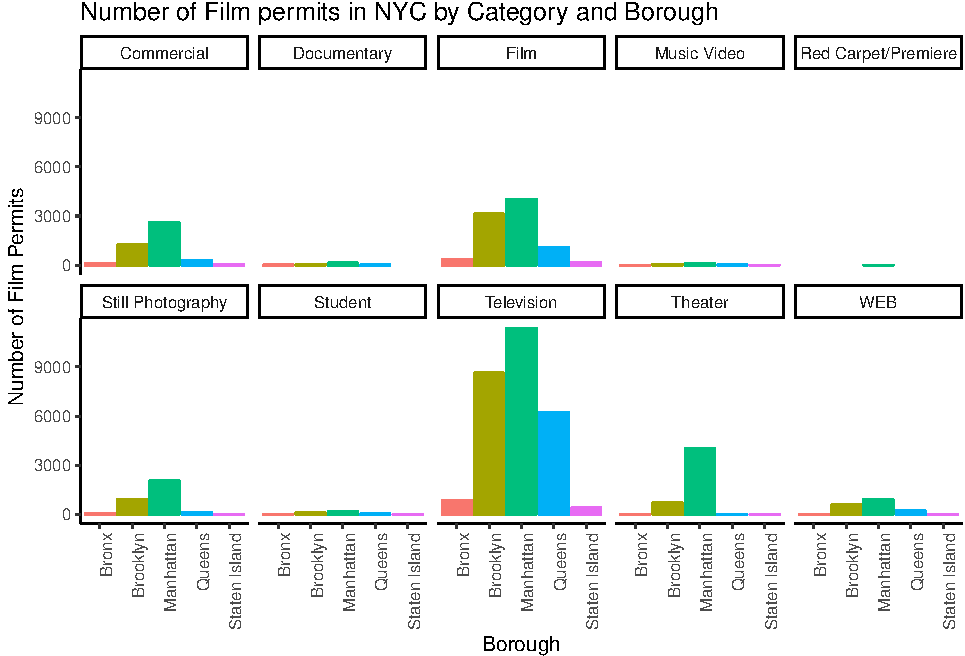
\includegraphics{Programming_Crump_files/figure-latex/unnamed-chunk-21-1.pdf}

\subsection{Gapminder Data}\label{gapminder-data}

\url{https://www.gapminder.org} is an organization that collects some
really interesting worldwide data. They also make cool visualization
tools for looking at the data. There are many neat examples, and they
have visualization tools built right into their website that you can
play around with \url{https://www.gapminder.org/tools/}. That's fun
check it out.

There is also an R package called \texttt{gapminder}. When you install
this package, it loads in some of the data from gapminder, so we can
play with it in R.

If you don't have the gapminder package installed, you can install it by
running this code

\begin{Shaded}
\begin{Highlighting}[]
\KeywordTok{install.packages}\NormalTok{(}\StringTok{"gapminder"}\NormalTok{)}
\end{Highlighting}
\end{Shaded}

Once the package is installed, you need to load the new library, like
this. Then, you can put the \texttt{gapminder} data into a data frame,
like we do here: \texttt{gapminder\_df}.

\begin{Shaded}
\begin{Highlighting}[]
\KeywordTok{library}\NormalTok{(gapminder)}
\NormalTok{gapminder_df<-gapminder}
\end{Highlighting}
\end{Shaded}

\subsubsection{Look at the data frame}\label{look-at-the-data-frame}

You can look at the data frame to see what is in it, and you can use
\texttt{summarytools} again to view a summary of the data.

\begin{Shaded}
\begin{Highlighting}[]
\KeywordTok{view}\NormalTok{(}\KeywordTok{dfSummary}\NormalTok{(gapminder_df))}
\end{Highlighting}
\end{Shaded}

There are 1704 rows of data, and we see some columns for country,
continent, year, life expectancy, population, and GDP per capita.

\subsection{Asking Questions with the gap minder
data}\label{asking-questions-with-the-gap-minder-data}

We will show you how to graph some the data to answer a few different
kinds of questions. Then you will form your own questions, and see if
you can answer them with ggplot2 yourself. All you will need to do is
copy and paste the following examples, and change them up a little bit

\subsubsection{Life Expectancy
histogram}\label{life-expectancy-histogram}

How long are people living all around the world according to this data
set? There are many ways we could plot the data to find out. The first
way is a histogram. We have many numbers for life expectancy in the
column \texttt{lifeExp}. This is a big sample, full of numbers for 142
countries across many years. It's easy to make a histogram in ggplot to
view the distribution:

\begin{Shaded}
\begin{Highlighting}[]
\KeywordTok{ggplot}\NormalTok{(gapminder_df, }\KeywordTok{aes}\NormalTok{(}\DataTypeTok{x=}\NormalTok{lifeExp))+}
\StringTok{  }\KeywordTok{geom_histogram}\NormalTok{(}\DataTypeTok{color=}\StringTok{"white"}\NormalTok{)}
\end{Highlighting}
\end{Shaded}

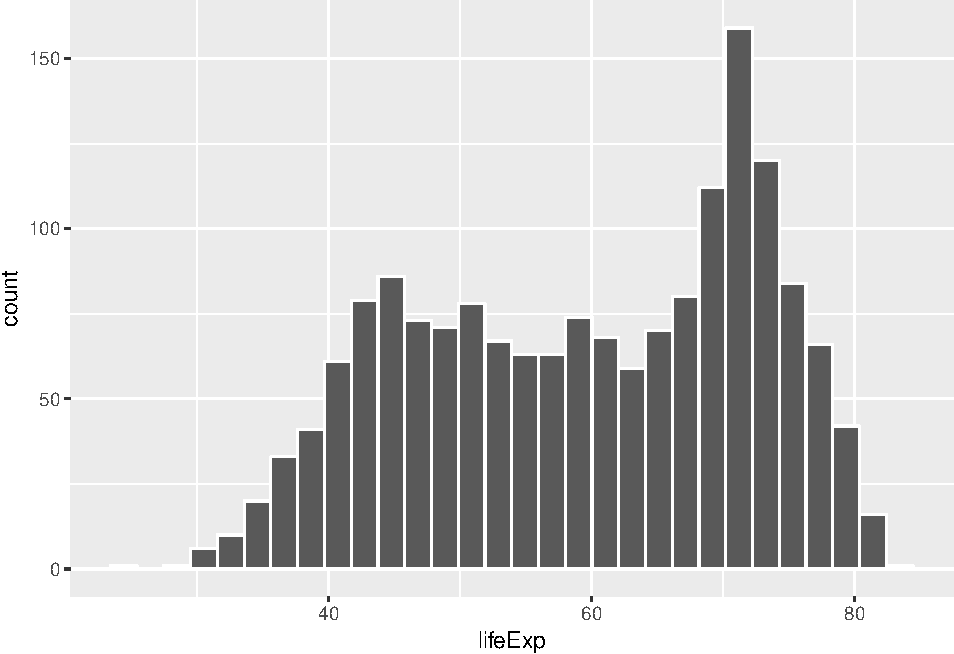
\includegraphics{Programming_Crump_files/figure-latex/unnamed-chunk-25-1.pdf}

See, that was easy. Next, is a code block that adds more layers and
settings if you wanted to modify parts of the graph:

\begin{Shaded}
\begin{Highlighting}[]
\KeywordTok{ggplot}\NormalTok{(gapminder_df, }\KeywordTok{aes}\NormalTok{(}\DataTypeTok{x =} \NormalTok{lifeExp)) +}
\StringTok{  }\KeywordTok{geom_histogram}\NormalTok{(}\DataTypeTok{color=}\StringTok{"white"}\NormalTok{)+}\StringTok{ }
\StringTok{  }\KeywordTok{theme_classic}\NormalTok{(}\DataTypeTok{base_size =} \DecValTok{15}\NormalTok{) +}
\StringTok{  }\KeywordTok{ylab}\NormalTok{(}\StringTok{"Frequency count"}\NormalTok{) +}\StringTok{ }
\StringTok{  }\KeywordTok{xlab}\NormalTok{(}\StringTok{"Life Expectancy"}\NormalTok{) +}
\StringTok{  }\KeywordTok{ggtitle}\NormalTok{(}\StringTok{"Histogram of Life Expectancy from Gapminder"}\NormalTok{)}
\end{Highlighting}
\end{Shaded}

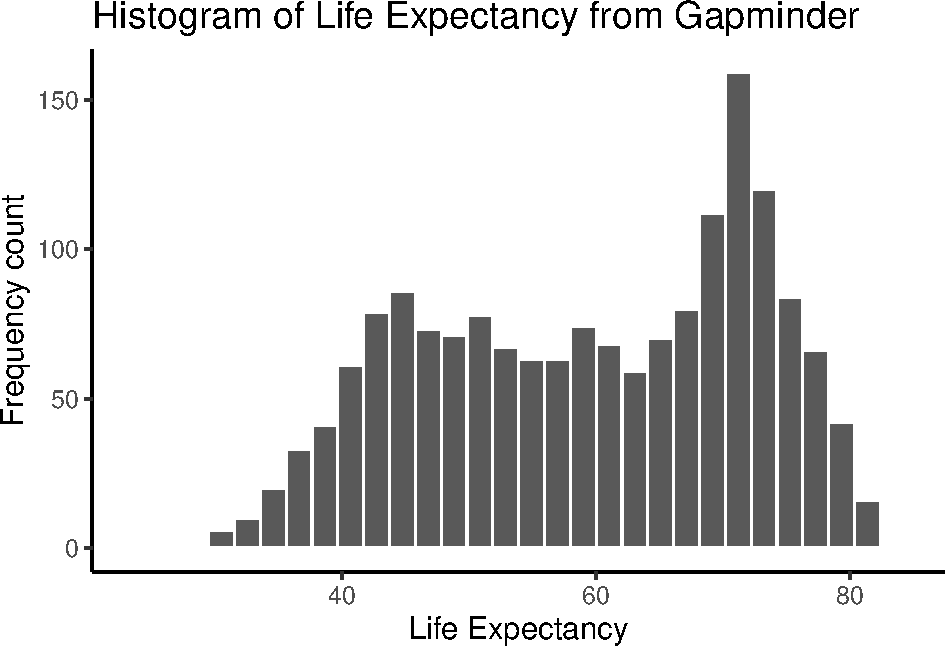
\includegraphics{Programming_Crump_files/figure-latex/unnamed-chunk-26-1.pdf}

The histogram shows a wide range of life expectancies, from below 40 to
just over 80. Histograms are useful, they can show you what kinds of
values happen more often than others.

One final thing about histograms in ggplot. You may want to change the
bin size. That controls how wide or narrow, or the number of bars (how
they split across the range), in the histogram. You need to set the
\texttt{bins=} option in \texttt{geom\_histogram()}.

\begin{Shaded}
\begin{Highlighting}[]
\KeywordTok{ggplot}\NormalTok{(gapminder_df, }\KeywordTok{aes}\NormalTok{(}\DataTypeTok{x =} \NormalTok{lifeExp)) +}
\StringTok{  }\KeywordTok{geom_histogram}\NormalTok{(}\DataTypeTok{color=}\StringTok{"white"}\NormalTok{, }\DataTypeTok{bins=}\DecValTok{50}\NormalTok{)+}\StringTok{ }
\StringTok{  }\KeywordTok{theme_classic}\NormalTok{(}\DataTypeTok{base_size =} \DecValTok{15}\NormalTok{) +}
\StringTok{  }\KeywordTok{ylab}\NormalTok{(}\StringTok{"Frequency count"}\NormalTok{) +}\StringTok{ }
\StringTok{  }\KeywordTok{xlab}\NormalTok{(}\StringTok{"Life Expectancy"}\NormalTok{) +}
\StringTok{  }\KeywordTok{ggtitle}\NormalTok{(}\StringTok{"Histogram of Life Expectancy from Gapminder"}\NormalTok{)}
\end{Highlighting}
\end{Shaded}

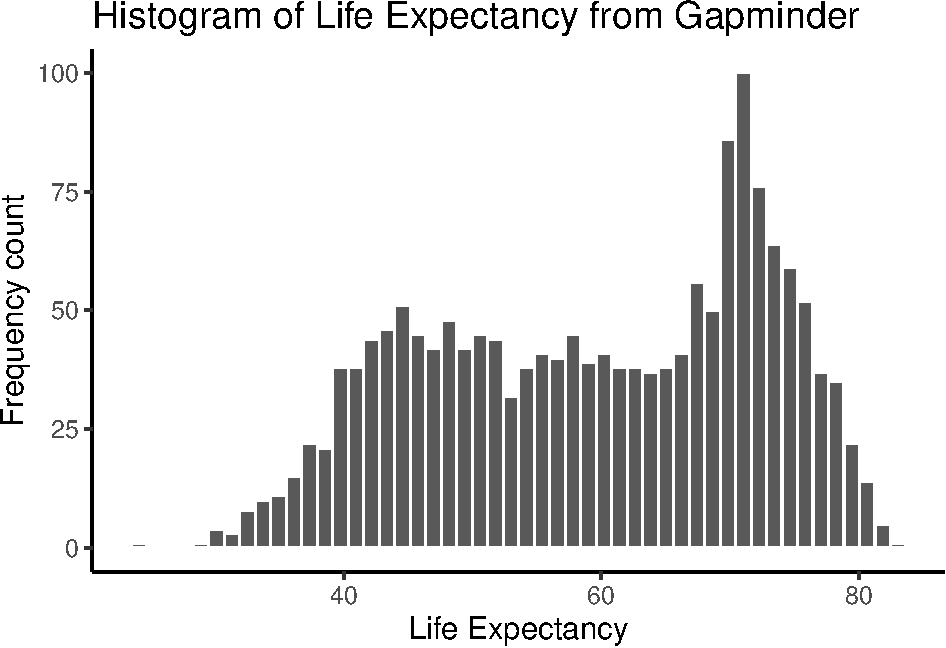
\includegraphics{Programming_Crump_files/figure-latex/unnamed-chunk-27-1.pdf}

See, same basic patter, but now breaking up the range into 50 little
equal sized bins, rather than 30, which is the default. You get to
choose what you want to do.

\subsubsection{Life Expectancy by year
Scatterplot}\label{life-expectancy-by-year-scatterplot}

We can see we have data for life expectancy and different years. So,
does worldwide life expectancy change across the years in the data set?
As we go into the future, are people living longer?

Let's look at this using a scatter plot. We can set the x-axis to be
year, and the y-axis to be life expectancy. Then we can use
\texttt{geom\_point()} to display a whole bunch of dots, and then look
at them. Here's the simple code:

\begin{Shaded}
\begin{Highlighting}[]
\KeywordTok{ggplot}\NormalTok{(gapminder_df, }\KeywordTok{aes}\NormalTok{(}\DataTypeTok{y=} \NormalTok{lifeExp, }\DataTypeTok{x=} \NormalTok{year))+}
\StringTok{  }\KeywordTok{geom_point}\NormalTok{()}
\end{Highlighting}
\end{Shaded}

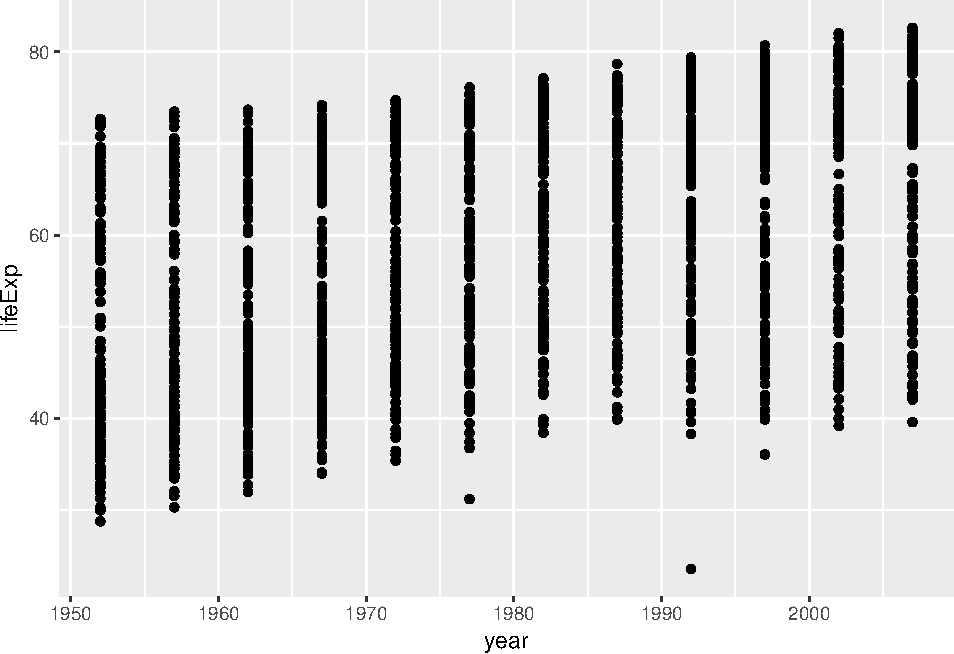
\includegraphics{Programming_Crump_files/figure-latex/unnamed-chunk-28-1.pdf}

Whoa, that's a lot of dots! Remember that each country is measured each
year. So, the bands of dots you see, show the life expectancies for the
whole range of countries within each year of the database. There is a
big spread inside each year. But, on the whole it looks like groups of
dots slowly go up over years.

\subsubsection{One country, life expectancy by
year}\label{one-country-life-expectancy-by-year}

I'm (Matt) from Canada, so maybe I want to know if life expectancy for
Canadians is going up over the years. To find out the answer for one
country, we first need to split the full data set, into another smaller
data set that only contains data for Canada. In other words, we want
only the rows where the word ``Canada'' is found in the \texttt{country}
column. We will use the \texttt{filter} function from \texttt{dplyr} for
this:

\begin{Shaded}
\begin{Highlighting}[]
\CommentTok{# filter rows to contain Canada}

\NormalTok{smaller_df <-}\StringTok{ }\NormalTok{gapminder_df %>%}\StringTok{ }
\StringTok{                 }\KeywordTok{filter}\NormalTok{(country ==}\StringTok{ "Canada"}\NormalTok{)}

\CommentTok{# plot the new data contained in smaller_df}

\KeywordTok{ggplot}\NormalTok{(smaller_df, }\KeywordTok{aes}\NormalTok{(}\DataTypeTok{y=} \NormalTok{lifeExp, }\DataTypeTok{x=} \NormalTok{year))+}
\StringTok{  }\KeywordTok{geom_point}\NormalTok{()}
\end{Highlighting}
\end{Shaded}

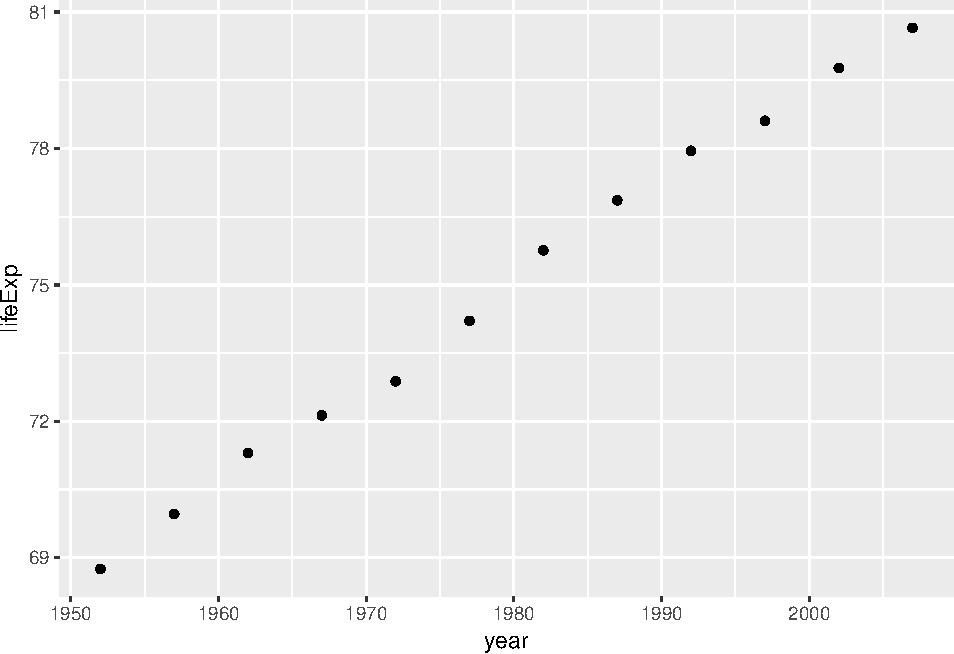
\includegraphics{Programming_Crump_files/figure-latex/unnamed-chunk-29-1.pdf}

I would say things are looking good for Canadians, their life expectancy
is going up over the years!

\subsubsection{Multiple countries
scatterplot}\label{multiple-countries-scatterplot}

What if we want to look at a few countries altogether. We can do this
too. We just change how we filter the data so more than one country is
allowed, then we plot the data. We will also add some nicer color
options and make the plot look pretty. First, the simple code:

\begin{Shaded}
\begin{Highlighting}[]
\CommentTok{# filter rows to contain countries of choice}

\NormalTok{smaller_df <-}\StringTok{ }\NormalTok{gapminder_df %>%}\StringTok{ }
\StringTok{                 }\KeywordTok{filter}\NormalTok{(country %in%}\StringTok{ }\KeywordTok{c}\NormalTok{(}\StringTok{"Canada"}\NormalTok{,}\StringTok{"France"}\NormalTok{,}\StringTok{"Brazil"}\NormalTok{) ==}\StringTok{ }\OtherTok{TRUE}\NormalTok{)}

\CommentTok{# plot the new data contained in smaller_df}

\KeywordTok{ggplot}\NormalTok{(smaller_df, }\KeywordTok{aes}\NormalTok{(}\DataTypeTok{y=} \NormalTok{lifeExp, }\DataTypeTok{x=} \NormalTok{year, }\DataTypeTok{group=} \NormalTok{country))+}
\StringTok{  }\KeywordTok{geom_point}\NormalTok{()}
\end{Highlighting}
\end{Shaded}

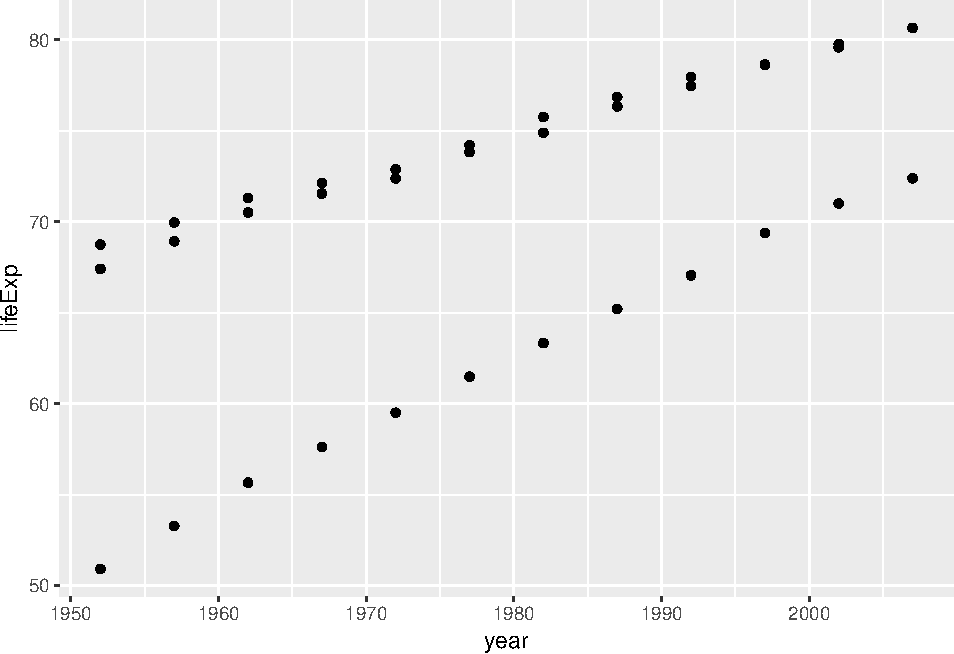
\includegraphics{Programming_Crump_files/figure-latex/unnamed-chunk-30-1.pdf}

Nice, we can now see three sets of dots, but which are countries do they
represent? Let's add a legend, and make the graph better looking.

\begin{Shaded}
\begin{Highlighting}[]
\KeywordTok{ggplot}\NormalTok{(smaller_df,}\KeywordTok{aes}\NormalTok{(}\DataTypeTok{y=} \NormalTok{lifeExp, }\DataTypeTok{x=} \NormalTok{year, }
                      \DataTypeTok{group=} \NormalTok{country, }\DataTypeTok{color =} \NormalTok{country)) +}
\StringTok{  }\KeywordTok{geom_point}\NormalTok{()+}\StringTok{ }
\StringTok{  }\KeywordTok{theme_classic}\NormalTok{(}\DataTypeTok{base_size =} \DecValTok{15}\NormalTok{) +}
\StringTok{  }\KeywordTok{ylab}\NormalTok{(}\StringTok{"Life Expectancy"}\NormalTok{) +}\StringTok{ }
\StringTok{  }\KeywordTok{xlab}\NormalTok{(}\StringTok{"Year"}\NormalTok{) +}
\StringTok{  }\KeywordTok{ggtitle}\NormalTok{(}\StringTok{"Life expectancy by year for three countries"}\NormalTok{)}
\end{Highlighting}
\end{Shaded}

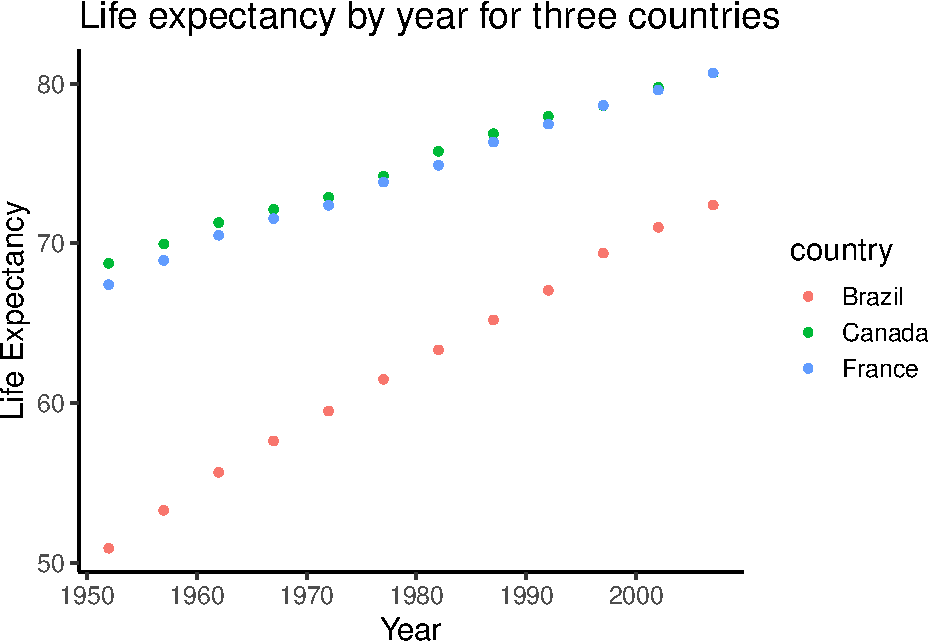
\includegraphics{Programming_Crump_files/figure-latex/unnamed-chunk-31-1.pdf}

\subsubsection{geom\_line() connecting the
dots}\label{geom_line-connecting-the-dots}

We might also want to connect the dots with a line, to make it easier to
see the connection! Remember, ggplot2 draws layers on top of layers. So,
we add in a new \texttt{geom\_line()} layer.

\begin{Shaded}
\begin{Highlighting}[]
\KeywordTok{ggplot}\NormalTok{(smaller_df,}\KeywordTok{aes}\NormalTok{(}\DataTypeTok{y=} \NormalTok{lifeExp, }\DataTypeTok{x=} \NormalTok{year, }
                      \DataTypeTok{group=} \NormalTok{country, }\DataTypeTok{color =} \NormalTok{country)) +}
\StringTok{  }\KeywordTok{geom_point}\NormalTok{()+}\StringTok{ }
\StringTok{  }\KeywordTok{geom_line}\NormalTok{()+}
\StringTok{  }\KeywordTok{theme_classic}\NormalTok{(}\DataTypeTok{base_size =} \DecValTok{15}\NormalTok{) +}
\StringTok{  }\KeywordTok{ylab}\NormalTok{(}\StringTok{"Life Expectancy"}\NormalTok{) +}\StringTok{ }
\StringTok{  }\KeywordTok{xlab}\NormalTok{(}\StringTok{"Year"}\NormalTok{) +}
\StringTok{  }\KeywordTok{ggtitle}\NormalTok{(}\StringTok{"Life expectancy by year for three countries"}\NormalTok{)}
\end{Highlighting}
\end{Shaded}

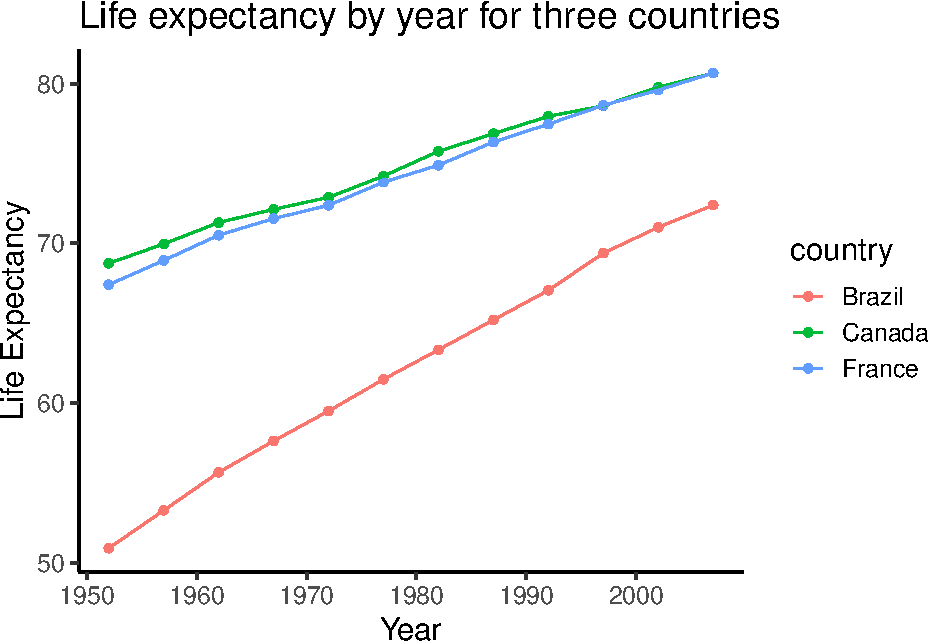
\includegraphics{Programming_Crump_files/figure-latex/unnamed-chunk-32-1.pdf}

Whenever you have a variable with multiple numbers, you can always plot
it, just like in the above example. Remember the variable
\emph{my\_numbers} contains 100 numbers. This means there are 100 slots
in the variable. Each slot has an \emph{index} value. The index value
for the first slot is 1, the index value for the second slot is 2, and
so on. The x-axis (the bottom line in the graph) shows the index value
from 1 to 100. Remember also, that each slot contains the number 43. The
y-axis (the vertical line in the graph) shows a range of numbers. The
dots in the graph represent the value inside each slot of the variable.
Because each slot contains the value 43, we see all 100 dots, all in a
line, all positioned at 43 with respect to the y-axis.

Let's plot some of the other variables we made.

\begin{Shaded}
\begin{Highlighting}[]
\KeywordTok{plot}\NormalTok{(my_sequence)}
\end{Highlighting}
\end{Shaded}

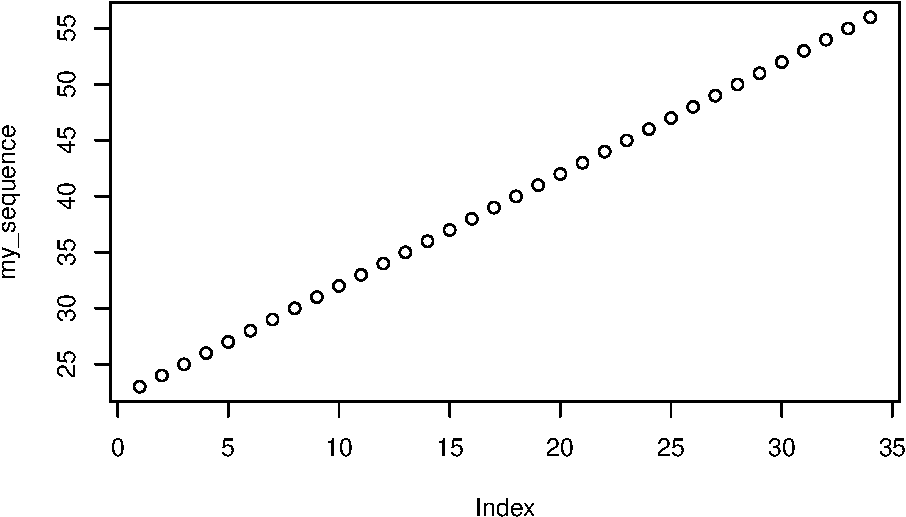
\includegraphics{Programming_Crump_files/figure-latex/unnamed-chunk-44-1.pdf}

The variable \emph{my\_sequence} contains the numbers 23 to 56, going up
by one. We see in the plot, the first number (on the x-axis) is a 23 on
the y-axis. As we go across the x-axis, the numbers go up by one until
we get to 56. We see a straight diagonal line.

\begin{Shaded}
\begin{Highlighting}[]
\KeywordTok{plot}\NormalTok{(my_randoms)}
\end{Highlighting}
\end{Shaded}

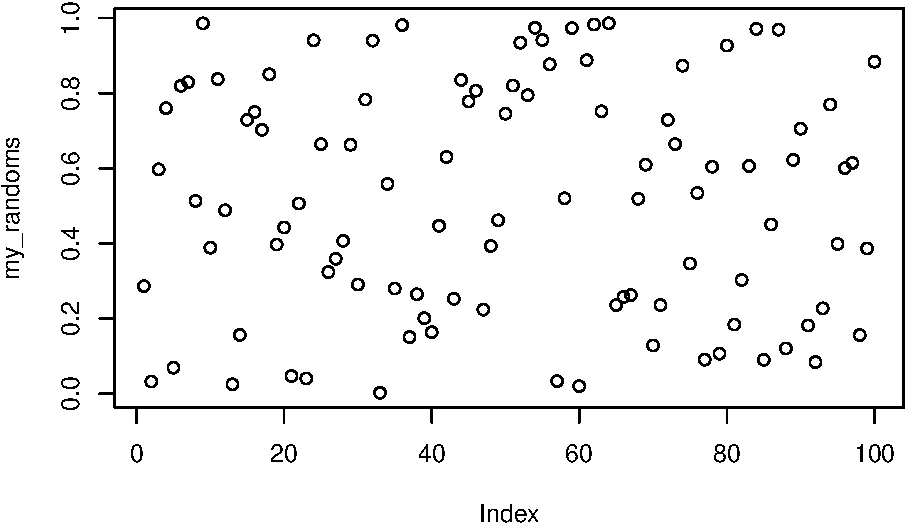
\includegraphics{Programming_Crump_files/figure-latex/unnamed-chunk-45-1.pdf}

The variable \emph{my\_randoms} contains 100 random numbers between 0
and 1. The plot shows dots all over the place between 0 and 1 on the
y-axis.

\begin{Shaded}
\begin{Highlighting}[]
\KeywordTok{plot}\NormalTok{(my_normal)}
\end{Highlighting}
\end{Shaded}

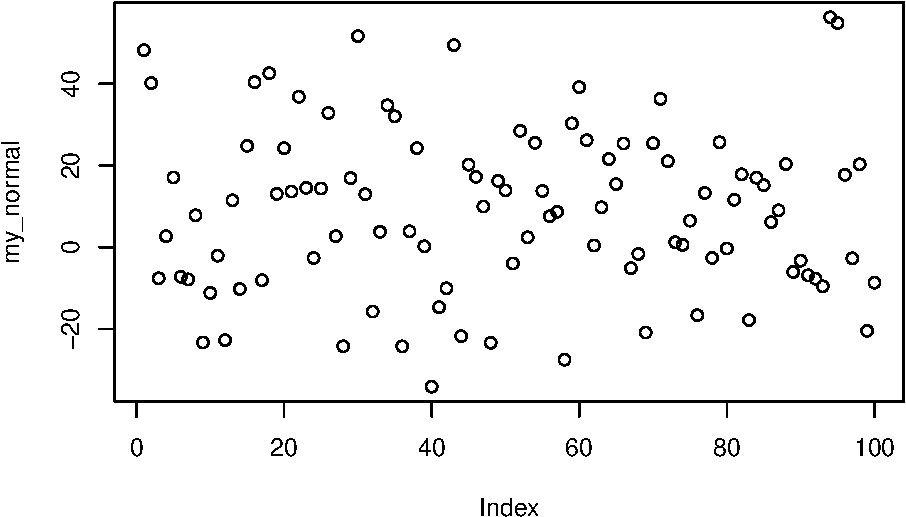
\includegraphics{Programming_Crump_files/figure-latex/unnamed-chunk-46-1.pdf}

The variable \emph{my\_normal} contains 100 numbers sample from a normal
distribution with a mean of 10, and a standard deviation of 20. Roughly,
most of the numbers should be close to 10, some of the numbers will be
greater and smaller than 10. But, as the numbers move away from 10 in
either direction, really small or really big numbers should occur less
and less frequently. We can sort of see this in the plot. For example,
you might notice that most the numbers are near the horizontal middle of
the graph, near the 10 on the y-axis, and less of the numbers are near
the top or bottom of the graph.

\subsubsection{Histograms}\label{histograms}

Histograms are used to visually summarize a set of numbers. In
particular, histograms split a set of numbers into bins, and then show
how many numbers fall within each bin. Each bin represents a pre-defined
range.

Let's create a set of numbers made up from 1s, 2s, and 3s. Let's say we
have ten 1s, twenty 2s, and 30 3s.

\begin{Shaded}
\begin{Highlighting}[]
\NormalTok{my_set <-}\StringTok{ }\KeywordTok{c}\NormalTok{(}\KeywordTok{rep}\NormalTok{(}\DecValTok{1}\NormalTok{,}\DecValTok{10}\NormalTok{),}\KeywordTok{rep}\NormalTok{(}\DecValTok{2}\NormalTok{,}\DecValTok{20}\NormalTok{),}\KeywordTok{rep}\NormalTok{(}\DecValTok{3}\NormalTok{,}\DecValTok{30}\NormalTok{))}
\end{Highlighting}
\end{Shaded}

The above line of code uses two R functions, rep(), and c(). We already
know how rep works. The c() function is short for combine. So, the above
line of code, combines 10 1s, 20 2s and 30 3s, all into one variable.
The contents of the variable looks like this:

\begin{Shaded}
\begin{Highlighting}[]
\NormalTok{my_set}
\end{Highlighting}
\end{Shaded}

\begin{verbatim}
##  [1] 1 1 1 1 1 1 1 1 1 1 2 2 2 2 2 2 2 2 2 2 2 2 2 2 2 2 2 2 2 2 3 3 3 3 3
## [36] 3 3 3 3 3 3 3 3 3 3 3 3 3 3 3 3 3 3 3 3 3 3 3 3 3
\end{verbatim}

Because, we made this variable, we already know what is inside it. Let's
make a histogram of the variable, to see what that looks like:

\begin{Shaded}
\begin{Highlighting}[]
\KeywordTok{hist}\NormalTok{(my_set)}
\end{Highlighting}
\end{Shaded}

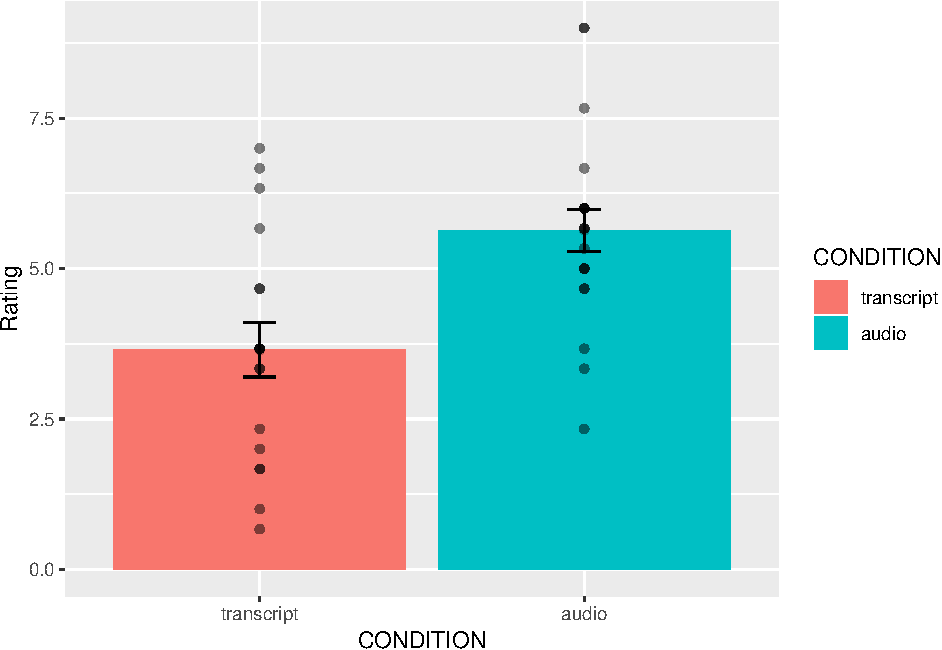
\includegraphics{Programming_Crump_files/figure-latex/unnamed-chunk-49-1.pdf}

The histogram is a bar graph. The height of each bar represents a count,
or the frequency of how many numbers fall inside each bin. The x-axis
shows the bin ranges. If you do not specify the bin ranges, then R will
make a reasonable guess for you. In this case, R set the bin ranges in
steps of .5. For example, 1-1.5, 1.5-2, 2-2.5, 2.5-3. R uses the word
\emph{breaks} to refer to bins. And, when you plot a histogram, you can
set your own breaks, or bin ranges.

\begin{Shaded}
\begin{Highlighting}[]
\KeywordTok{hist}\NormalTok{(my_set, }\DataTypeTok{breaks=}\KeywordTok{c}\NormalTok{(}\DecValTok{0}\NormalTok{,}\DecValTok{1}\NormalTok{,}\DecValTok{2}\NormalTok{,}\DecValTok{3}\NormalTok{,}\DecValTok{4}\NormalTok{))}
\end{Highlighting}
\end{Shaded}

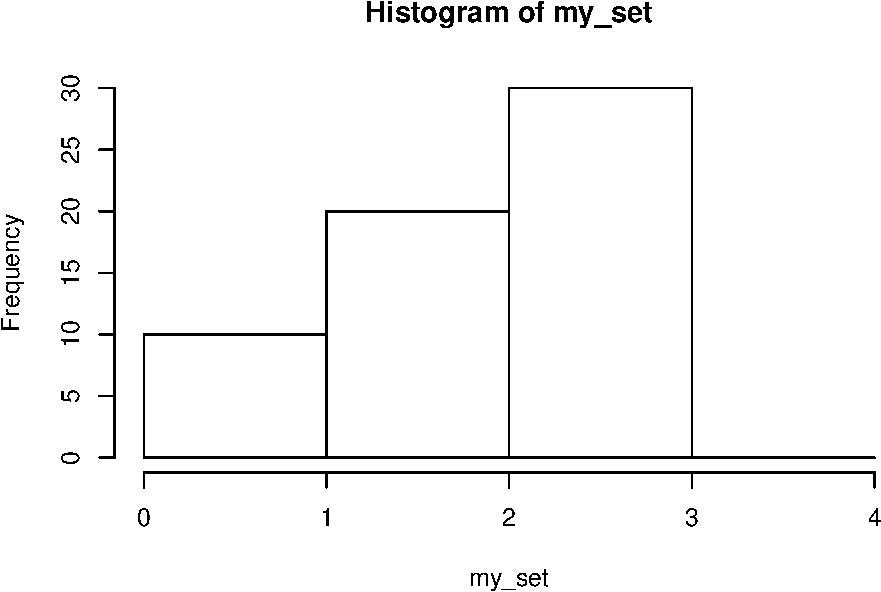
\includegraphics{Programming_Crump_files/figure-latex/unnamed-chunk-50-1.pdf}

Let's spend a moment interpreting this new histogram. The first bar is
between 0 and 1 on the x-axis, and has a value of 10 on the y-axis. This
means that there are 10 numbers inside the my\_set variable that have a
value between 0 and 1; specifically, a value greater than zero up to and
equalling 1. The second bar is between 1 and 2 on the x-axis, and has a
value of 20 on the y-axis. So, there are 20 numbers in the variable with
a value greater than 1 up to and equalling 2. Finally, the third bar
shows there are 30 numbers in the range greater than 2, up to equalling
3. We can also see there are no numbers smaller than 0, or greater than
4.

\subsubsection{What are histograms useful
for?}\label{what-are-histograms-useful-for}

A primary purpose of histograms is to get a quick look at the range and
frequency of a set of numbers. In particular, when the bars are of
different sizes, we can know that some values occur more than others.

What should a histogram look like for a set of values whose numbers all
occur randomly, and equally frequently? By this definition, we are
saying that all numbers, within all ranges, occur equally often. For
example, imagine we created a set of 10,000 numbers, and chose those
numbers from between 1 and 10, such that any number between 1 and 10
occurs with the same frequency as all other numbers. We can use the
random number generator and histogram to find out:

\begin{Shaded}
\begin{Highlighting}[]
\NormalTok{some_random_numbers <-}\StringTok{ }\KeywordTok{runif}\NormalTok{(}\DecValTok{10000}\NormalTok{,}\DecValTok{1}\NormalTok{,}\DecValTok{10}\NormalTok{)}
\KeywordTok{hist}\NormalTok{(some_random_numbers,}\DataTypeTok{breaks=}\KeywordTok{seq}\NormalTok{(}\DecValTok{0}\NormalTok{,}\DecValTok{11}\NormalTok{,}\DecValTok{1}\NormalTok{))}
\end{Highlighting}
\end{Shaded}

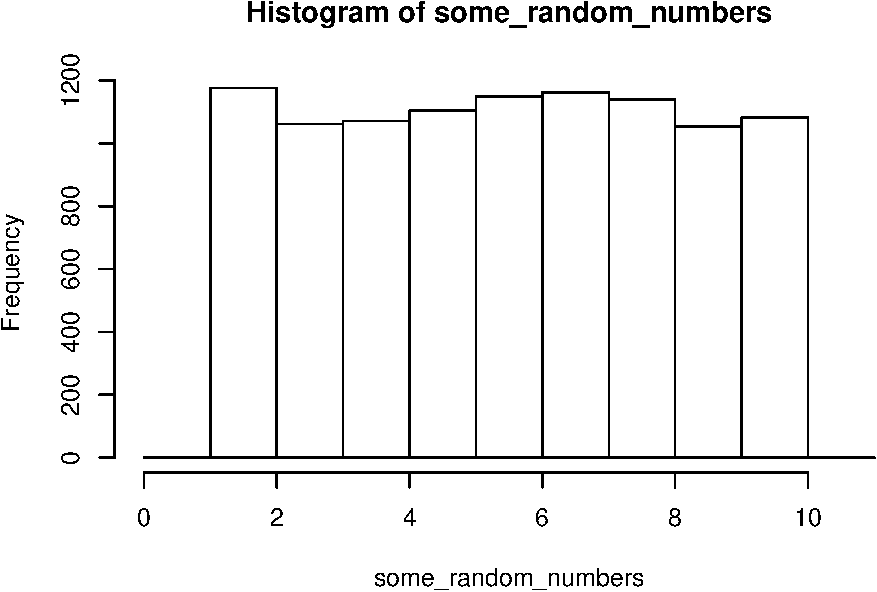
\includegraphics{Programming_Crump_files/figure-latex/unnamed-chunk-51-1.pdf}

\begin{Shaded}
\begin{Highlighting}[]
\CommentTok{#notice I set the breaks using the seq() function}
\end{Highlighting}
\end{Shaded}

We see that heights of the bars are all close to the same number. This
is good, because each number between 1 to 10 should have had an equal
chance of being selected. However, notice the bars are not exactly the
same height. This shows that the random number generator did actually
generate each number with equal frequency.

What about sets of numbers where some kinds of numbers occur more than
others? Here, we would expect higher bars for ranges containing many
values, and smaller numbers for ranges containing fewer values.

Let's plot histogram for a normal distribution and see what it looks
like. We will set the mean to 100, and the standard deviation to 20, and
we ask R to generate 10000 numbers from this distribution.

\begin{Shaded}
\begin{Highlighting}[]
\NormalTok{normal_sample <-}\StringTok{ }\KeywordTok{rnorm}\NormalTok{(}\DecValTok{10000}\NormalTok{,}\DecValTok{100}\NormalTok{,}\DecValTok{20}\NormalTok{)}
\KeywordTok{hist}\NormalTok{(normal_sample)}
\end{Highlighting}
\end{Shaded}

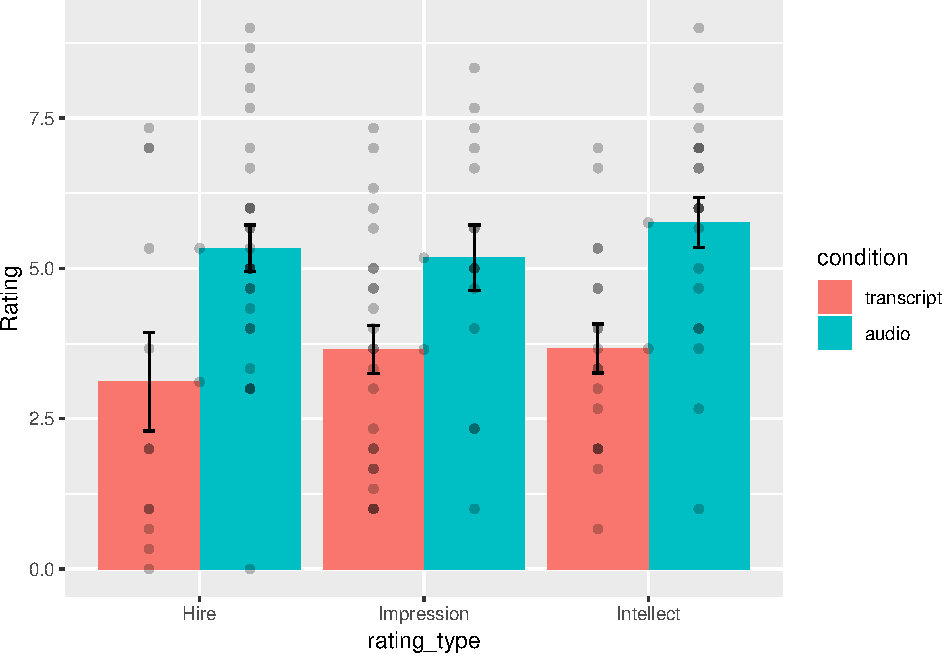
\includegraphics{Programming_Crump_files/figure-latex/unnamed-chunk-52-1.pdf}
The histogram shows that the highest bars are in the middle, near the
100 mark. So, numbers near 100 occured most frequently in our set. What
happens to the heights of the bars on either side of the histogram? The
bars are decreasing in height as they move away from the middle in both
directions. So, as numbers move away from 100, they occur less and less
frequently. For example, we don't see any bars in the range of 500 or
1000. This means that no values that high were in our set of numbers.
From the histogram, we can clearly see that our set hardly had any
numbers greater than 150, or less than 50. Or, in other words, most of
the numbers were between 50 and 150.

--\textgreater{}

\section{Excel}\label{excel}

\section{SPSS}\label{spss}

\section{JAMOVI}\label{jamovi}

\chapter{Lab 2: Descriptive
Statistics}\label{lab-2-descriptive-statistics}

{ Some inspiring quote ---Inspiring Person }

\section{Outline of Problem to solve}\label{outline-of-problem-to-solve}

Stuff we need to say in general

\subsection{important things}\label{important-things}

Other things to say

\section{R}\label{r-2}

\subsection{Descriptives basics in R}\label{descriptives-basics-in-r}

We learned in lecture and from the textbook that data we want to use ask
and answer questions often comes with loads of numbers. Too many numbers
to look at all at once. That's one reason we use descriptive statistics.
To reduce the big set of numbers to one or two summary numbers that tell
use something about all of the numbers. R can produce descriptive
statistics for you in many ways. There are base functions for most of
the ones that you want. We'll go over some R basics for descriptive
statistics, and then use our new found skills to ask some questions
about real data.

\subsubsection{Making numbers in R}\label{making-numbers-in-r}

In order to do descriptive statistics we need to put some numbers in a
variable. You can also do this using the \texttt{c()} command, which
stands for combine

\begin{Shaded}
\begin{Highlighting}[]
\NormalTok{my_numbers <-}\StringTok{ }\KeywordTok{c}\NormalTok{(}\DecValTok{1}\NormalTok{,}\DecValTok{2}\NormalTok{,}\DecValTok{3}\NormalTok{,}\DecValTok{4}\NormalTok{)}
\end{Highlighting}
\end{Shaded}

There a few other handy ways to make numbers. We can use \texttt{seq()}
to make a sequence. Here's making the numbers from 1 to 100

\begin{Shaded}
\begin{Highlighting}[]
\NormalTok{one_to_one_hundred <-}\StringTok{ }\KeywordTok{seq}\NormalTok{(}\DecValTok{1}\NormalTok{,}\DecValTok{100}\NormalTok{,}\DecValTok{1}\NormalTok{)}
\end{Highlighting}
\end{Shaded}

We can repeat things, using rep. Here's making 10 5s, and 25 1s:

\begin{Shaded}
\begin{Highlighting}[]
\KeywordTok{rep}\NormalTok{(}\DecValTok{10}\NormalTok{,}\DecValTok{5}\NormalTok{)}
\end{Highlighting}
\end{Shaded}

\begin{verbatim}
## [1] 10 10 10 10 10
\end{verbatim}

\begin{Shaded}
\begin{Highlighting}[]
\KeywordTok{rep}\NormalTok{(}\DecValTok{1}\NormalTok{,}\DecValTok{25}\NormalTok{)}
\end{Highlighting}
\end{Shaded}

\begin{verbatim}
##  [1] 1 1 1 1 1 1 1 1 1 1 1 1 1 1 1 1 1 1 1 1 1 1 1 1 1
\end{verbatim}

\begin{Shaded}
\begin{Highlighting}[]
\NormalTok{all_together_now <-}\StringTok{ }\KeywordTok{c}\NormalTok{(}\KeywordTok{rep}\NormalTok{(}\DecValTok{10}\NormalTok{,}\DecValTok{5}\NormalTok{),}\KeywordTok{rep}\NormalTok{(}\DecValTok{1}\NormalTok{,}\DecValTok{25}\NormalTok{)) }
\end{Highlighting}
\end{Shaded}

\subsubsection{Sum}\label{sum}

Let's play with the number 1 to 100. First, let's use the \texttt{sum()}
function to add them up

\begin{Shaded}
\begin{Highlighting}[]
\NormalTok{one_to_one_hundred <-}\StringTok{ }\KeywordTok{seq}\NormalTok{(}\DecValTok{1}\NormalTok{,}\DecValTok{100}\NormalTok{,}\DecValTok{1}\NormalTok{)}
\KeywordTok{sum}\NormalTok{(one_to_one_hundred)}
\end{Highlighting}
\end{Shaded}

\begin{verbatim}
## [1] 5050
\end{verbatim}

\subsubsection{Length}\label{length}

We put 100 numbers into the variable \texttt{one\_to\_one\_hundred}. We
know how many numbers there are in there. How can we get R to tell us?
We use \texttt{length()} for that.

\begin{Shaded}
\begin{Highlighting}[]
\KeywordTok{length}\NormalTok{(one_to_one_hundred)}
\end{Highlighting}
\end{Shaded}

\begin{verbatim}
## [1] 100
\end{verbatim}

\subsection{Central Tendency}\label{central-tendency}

\subsubsection{Mean}\label{mean}

Remember the mean of some numbers is their sum, divided by the number of
numbers. We can compute the mean like this:

\begin{Shaded}
\begin{Highlighting}[]
\KeywordTok{sum}\NormalTok{(one_to_one_hundred)/}\KeywordTok{length}\NormalTok{(one_to_one_hundred)}
\end{Highlighting}
\end{Shaded}

\begin{verbatim}
## [1] 50.5
\end{verbatim}

Or, we could just use the \texttt{mean()} function like this:

\begin{Shaded}
\begin{Highlighting}[]
\KeywordTok{mean}\NormalTok{(one_to_one_hundred)}
\end{Highlighting}
\end{Shaded}

\begin{verbatim}
## [1] 50.5
\end{verbatim}

\subsubsection{Median}\label{median}

The median is the number in the exact middle of the numbers ordered from
smallest to largest. If there are an even number of numbers (no number
in the middle), then we take the number in between the two (decimal .5).
Use the \texttt{median} function. There's only 3 numbers here. The
middle one is 2, that should be the median

\begin{Shaded}
\begin{Highlighting}[]
\KeywordTok{median}\NormalTok{(}\KeywordTok{c}\NormalTok{(}\DecValTok{1}\NormalTok{,}\DecValTok{2}\NormalTok{,}\DecValTok{3}\NormalTok{))}
\end{Highlighting}
\end{Shaded}

\begin{verbatim}
## [1] 2
\end{verbatim}

\subsubsection{Mode}\label{mode}

R does not a base function for the Mode. You would have to write one for
yourself. Here is an example of writing your own mode function, and then
using it. Note I searched how to do this on Google, and am using the
mode defined by
\href{https://stackoverflow.com/questions/2547402/is-there-a-built-in-function-for-finding-the-mode}{this
answer on stack overflow}

Remember, the mode is the most frequently occurring number in the set.
Below 1 occurs the most, so the mode will be one.

\begin{Shaded}
\begin{Highlighting}[]
\NormalTok{my_mode <-}\StringTok{ }\NormalTok{function(x) \{}
  \NormalTok{ux <-}\StringTok{ }\KeywordTok{unique}\NormalTok{(x)}
  \NormalTok{ux[}\KeywordTok{which.max}\NormalTok{(}\KeywordTok{tabulate}\NormalTok{(}\KeywordTok{match}\NormalTok{(x, ux)))]}
\NormalTok{\}}

\KeywordTok{my_mode}\NormalTok{(}\KeywordTok{c}\NormalTok{(}\DecValTok{1}\NormalTok{,}\DecValTok{1}\NormalTok{,}\DecValTok{1}\NormalTok{,}\DecValTok{1}\NormalTok{,}\DecValTok{1}\NormalTok{,}\DecValTok{1}\NormalTok{,}\DecValTok{1}\NormalTok{,}\DecValTok{2}\NormalTok{,}\DecValTok{3}\NormalTok{,}\DecValTok{4}\NormalTok{))}
\end{Highlighting}
\end{Shaded}

\begin{verbatim}
## [1] 1
\end{verbatim}

\subsection{Variation}\label{variation}

We often want to know how variable the numbers are. We are going to look
at descriptive statistics to describe this such as the \textbf{range},
\textbf{variance}, the \textbf{standard deviation}, and a few others.

First, let's remind ourselves what variation looks like (it's when the
numbers are different). We will sample 100 numbers from a normal
distribution (don't worry about this yet), with a mean of 10, and a
standard deviation of 5, and then make a histogram so we can see the
variation around 10..

\begin{Shaded}
\begin{Highlighting}[]
\NormalTok{sample_numbers <-}\StringTok{ }\KeywordTok{rnorm}\NormalTok{(}\DecValTok{100}\NormalTok{,}\DecValTok{10}\NormalTok{,}\DecValTok{5}\NormalTok{)}
\KeywordTok{hist}\NormalTok{(sample_numbers)}
\end{Highlighting}
\end{Shaded}

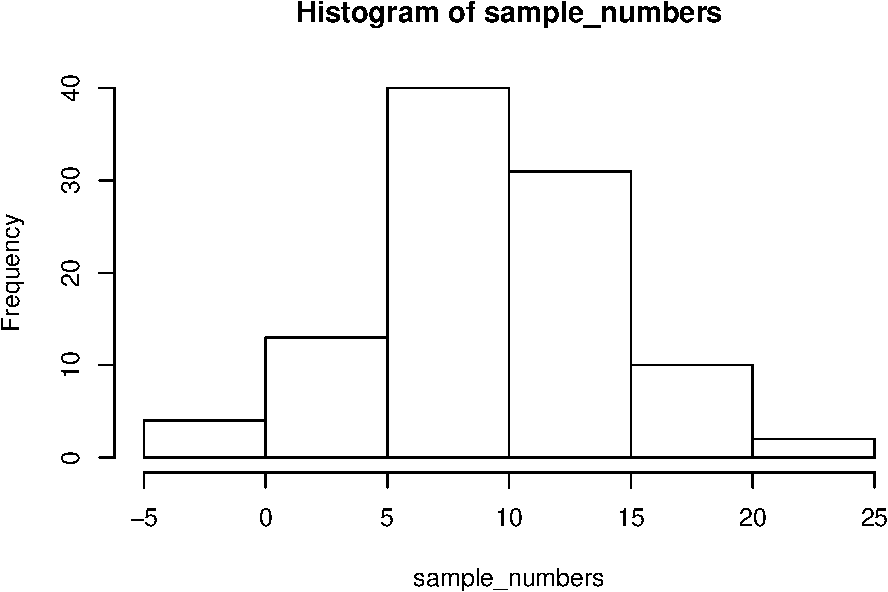
\includegraphics{Programming_Crump_files/figure-latex/unnamed-chunk-62-1.pdf}

\subsubsection{range}\label{range}

The range is the minimum and maximum values in the set, we use the
\texttt{range} function.

\begin{Shaded}
\begin{Highlighting}[]
\KeywordTok{range}\NormalTok{(sample_numbers)}
\end{Highlighting}
\end{Shaded}

\begin{verbatim}
## [1] -3.670097 22.043840
\end{verbatim}

\subsubsection{var = variance}\label{var-variance}

We can find the sample variance using \texttt{var}. Note, divides by
(n-1)

\begin{Shaded}
\begin{Highlighting}[]
\KeywordTok{var}\NormalTok{(sample_numbers)}
\end{Highlighting}
\end{Shaded}

\begin{verbatim}
## [1] 26.27427
\end{verbatim}

\subsubsection{sd = standard deviation}\label{sd-standard-deviation}

We find the sample standard deviation us SD. Note, divides by (n-1)

\begin{Shaded}
\begin{Highlighting}[]
\KeywordTok{sd}\NormalTok{(sample_numbers)}
\end{Highlighting}
\end{Shaded}

\begin{verbatim}
## [1] 5.125843
\end{verbatim}

Remember that the standard deviation is just the square root of the
variance, see:

\begin{Shaded}
\begin{Highlighting}[]
\KeywordTok{sqrt}\NormalTok{(}\KeywordTok{var}\NormalTok{(sample_numbers))}
\end{Highlighting}
\end{Shaded}

\begin{verbatim}
## [1] 5.125843
\end{verbatim}

\subsubsection{All Descriptives}\label{all-descriptives}

Let's put all of the descriptives and other functions so far in one
place:

\begin{Shaded}
\begin{Highlighting}[]
\NormalTok{sample_numbers <-}\StringTok{ }\KeywordTok{rnorm}\NormalTok{(}\DecValTok{100}\NormalTok{,}\DecValTok{10}\NormalTok{,}\DecValTok{5}\NormalTok{)}

\KeywordTok{sum}\NormalTok{(sample_numbers)}
\end{Highlighting}
\end{Shaded}

\begin{verbatim}
## [1] 988.536
\end{verbatim}

\begin{Shaded}
\begin{Highlighting}[]
\KeywordTok{length}\NormalTok{(sample_numbers)}
\end{Highlighting}
\end{Shaded}

\begin{verbatim}
## [1] 100
\end{verbatim}

\begin{Shaded}
\begin{Highlighting}[]
\KeywordTok{mean}\NormalTok{(sample_numbers)}
\end{Highlighting}
\end{Shaded}

\begin{verbatim}
## [1] 9.88536
\end{verbatim}

\begin{Shaded}
\begin{Highlighting}[]
\KeywordTok{median}\NormalTok{(sample_numbers)}
\end{Highlighting}
\end{Shaded}

\begin{verbatim}
## [1] 10.05067
\end{verbatim}

\begin{Shaded}
\begin{Highlighting}[]
\KeywordTok{my_mode}\NormalTok{(sample_numbers)}
\end{Highlighting}
\end{Shaded}

\begin{verbatim}
## [1] 8.865402
\end{verbatim}

\begin{Shaded}
\begin{Highlighting}[]
\KeywordTok{range}\NormalTok{(sample_numbers)}
\end{Highlighting}
\end{Shaded}

\begin{verbatim}
## [1] -1.710019 21.689287
\end{verbatim}

\begin{Shaded}
\begin{Highlighting}[]
\KeywordTok{var}\NormalTok{(sample_numbers)}
\end{Highlighting}
\end{Shaded}

\begin{verbatim}
## [1] 26.53768
\end{verbatim}

\begin{Shaded}
\begin{Highlighting}[]
\KeywordTok{sd}\NormalTok{(sample_numbers)}
\end{Highlighting}
\end{Shaded}

\begin{verbatim}
## [1] 5.151474
\end{verbatim}

\subsection{Descriptives by
conditions}\label{descriptives-by-conditions}

Sometimes you will have a single variable with some numbers, and you can
use the above functions to find the descriptives for that variable.
Other times (most often in this course), you will have a big data frame
of numbers, with different numbers in different conditions. You will
want to find descriptive statistics for each the sets of numbers inside
each of the conditions. Fortunately, this is where R really shines, it
does it all for you in one go.

Let's illustrate the problem. Here I make a date frame with 10 numbers
in each condition. There are 10 conditions, each labelled, A, B, C, D,
E, F, G, H, I, J.

\begin{Shaded}
\begin{Highlighting}[]
\NormalTok{scores <-}\StringTok{ }\KeywordTok{rnorm}\NormalTok{(}\DecValTok{100}\NormalTok{,}\DecValTok{10}\NormalTok{,}\DecValTok{5}\NormalTok{)}
\NormalTok{conditions <-}\StringTok{ }\KeywordTok{rep}\NormalTok{(}\KeywordTok{c}\NormalTok{(}\StringTok{"A"}\NormalTok{,}\StringTok{"B"}\NormalTok{,}\StringTok{"C"}\NormalTok{,}\StringTok{"D"}\NormalTok{,}\StringTok{"E"}\NormalTok{,}\StringTok{"F"}\NormalTok{,}\StringTok{"G"}\NormalTok{,}\StringTok{"H"}\NormalTok{,}\StringTok{"I"}\NormalTok{,}\StringTok{"J"}\NormalTok{), }\DataTypeTok{each =}\DecValTok{10}\NormalTok{)}
\NormalTok{my_df <-}\StringTok{ }\KeywordTok{data.frame}\NormalTok{(conditions,scores)}
\end{Highlighting}
\end{Shaded}

If you look at the \texttt{my\_df} data frame, you will see it has 100
rows, there are 10 rows for each condition with a label in the
\texttt{conditions} column, and 10 scores for each condition in the
\texttt{scores} column. What if you wanted to know the mean of the
scores in each condition? You would want to find 10 means.

The slow way to do it would be like this:

\begin{Shaded}
\begin{Highlighting}[]
\KeywordTok{mean}\NormalTok{(my_df[my_df$conditions==}\StringTok{"A"}\NormalTok{,]$scores)}
\end{Highlighting}
\end{Shaded}

\begin{verbatim}
## [1] 8.284299
\end{verbatim}

\begin{Shaded}
\begin{Highlighting}[]
\KeywordTok{mean}\NormalTok{(my_df[my_df$conditions==}\StringTok{"B"}\NormalTok{,]$scores)}
\end{Highlighting}
\end{Shaded}

\begin{verbatim}
## [1] 9.071022
\end{verbatim}

\begin{Shaded}
\begin{Highlighting}[]
\KeywordTok{mean}\NormalTok{(my_df[my_df$conditions==}\StringTok{"C"}\NormalTok{,]$scores)}
\end{Highlighting}
\end{Shaded}

\begin{verbatim}
## [1] 7.426698
\end{verbatim}

\begin{Shaded}
\begin{Highlighting}[]
\CommentTok{# and then keep going}
\end{Highlighting}
\end{Shaded}

Nobody wants to do that! Not, me I stopped doing it that way, you should
to.

\subsubsection{group\_by and summarise}\label{group_by-and-summarise}

We can easily do everything all at once using the \texttt{group\_by} and
\texttt{summarise} function from the \texttt{dplyr} package. Just watch

\begin{Shaded}
\begin{Highlighting}[]
\KeywordTok{library}\NormalTok{(dplyr)}

\NormalTok{my_df %>%}
\StringTok{  }\KeywordTok{group_by}\NormalTok{(conditions) %>%}
\StringTok{  }\KeywordTok{summarise}\NormalTok{(}\DataTypeTok{means =} \KeywordTok{mean}\NormalTok{(scores))}
\end{Highlighting}
\end{Shaded}

\begin{verbatim}
## # A tibble: 10 x 2
##    conditions means
##    <fct>      <dbl>
##  1 A           8.28
##  2 B           9.07
##  3 C           7.43
##  4 D           8.63
##  5 E           9.76
##  6 F           5.63
##  7 G           8.31
##  8 H           9.59
##  9 I          12.4 
## 10 J          11.9
\end{verbatim}

A couple things now. First, the print out of this was ugly. Let's fix
that. we put the results of our code into a new variable, then we use
\texttt{knitr::kable} to print it out nicely when we \texttt{knit} the
document

\begin{Shaded}
\begin{Highlighting}[]
\NormalTok{summary_df <-}\StringTok{ }\NormalTok{my_df %>%}
\StringTok{               }\KeywordTok{group_by}\NormalTok{(conditions) %>%}
\StringTok{               }\KeywordTok{summarise}\NormalTok{(}\DataTypeTok{means =} \KeywordTok{mean}\NormalTok{(scores))}

\NormalTok{knitr::}\KeywordTok{kable}\NormalTok{(summary_df)}
\end{Highlighting}
\end{Shaded}

\begin{tabular}{l|r}
\hline
conditions & means\\
\hline
A & 8.284299\\
\hline
B & 9.071022\\
\hline
C & 7.426698\\
\hline
D & 8.630906\\
\hline
E & 9.759095\\
\hline
F & 5.632737\\
\hline
G & 8.310846\\
\hline
H & 9.590302\\
\hline
I & 12.398364\\
\hline
J & 11.881236\\
\hline
\end{tabular}

\subsubsection{multiple descriptives}\label{multiple-descriptives}

The best thing about the \texttt{dplyr} method, is that we can add more
than one function, and we'll get more than one summary returned, all in
a nice format, let's add the standard deviation:

\begin{Shaded}
\begin{Highlighting}[]
\NormalTok{summary_df <-}\StringTok{ }\NormalTok{my_df %>%}
\StringTok{               }\KeywordTok{group_by}\NormalTok{(conditions) %>%}
\StringTok{               }\KeywordTok{summarise}\NormalTok{(}\DataTypeTok{means =} \KeywordTok{mean}\NormalTok{(scores),}
                         \DataTypeTok{sds =} \KeywordTok{sd}\NormalTok{(scores))}

\NormalTok{knitr::}\KeywordTok{kable}\NormalTok{(summary_df)}
\end{Highlighting}
\end{Shaded}

\begin{tabular}{l|r|r}
\hline
conditions & means & sds\\
\hline
A & 8.284299 & 5.718872\\
\hline
B & 9.071022 & 7.346908\\
\hline
C & 7.426698 & 5.403125\\
\hline
D & 8.630906 & 4.240390\\
\hline
E & 9.759095 & 3.664083\\
\hline
F & 5.632737 & 5.414865\\
\hline
G & 8.310846 & 5.754972\\
\hline
H & 9.590302 & 4.911016\\
\hline
I & 12.398364 & 3.911585\\
\hline
J & 11.881236 & 4.591293\\
\hline
\end{tabular}

We'll add the min and the max too:

\begin{Shaded}
\begin{Highlighting}[]
\NormalTok{summary_df <-}\StringTok{ }\NormalTok{my_df %>%}
\StringTok{               }\KeywordTok{group_by}\NormalTok{(conditions) %>%}
\StringTok{               }\KeywordTok{summarise}\NormalTok{(}\DataTypeTok{means =} \KeywordTok{mean}\NormalTok{(scores),}
                         \DataTypeTok{sds =} \KeywordTok{sd}\NormalTok{(scores),}
                         \DataTypeTok{min =} \KeywordTok{min}\NormalTok{(scores),}
                         \DataTypeTok{max =} \KeywordTok{max}\NormalTok{(scores))}

\NormalTok{knitr::}\KeywordTok{kable}\NormalTok{(summary_df)}
\end{Highlighting}
\end{Shaded}

\begin{tabular}{l|r|r|r|r}
\hline
conditions & means & sds & min & max\\
\hline
A & 8.284299 & 5.718872 & -0.9643942 & 18.47722\\
\hline
B & 9.071022 & 7.346908 & -2.5467949 & 19.96221\\
\hline
C & 7.426698 & 5.403125 & -1.9385197 & 16.58471\\
\hline
D & 8.630906 & 4.240390 & 2.7670265 & 16.26315\\
\hline
E & 9.759095 & 3.664083 & 2.6638108 & 17.19651\\
\hline
F & 5.632737 & 5.414865 & -3.2441815 & 14.16092\\
\hline
G & 8.310846 & 5.754972 & -0.6914890 & 20.09894\\
\hline
H & 9.590302 & 4.911016 & 1.8352048 & 18.73463\\
\hline
I & 12.398364 & 3.911585 & 8.6547700 & 19.84778\\
\hline
J & 11.881236 & 4.591293 & 5.9818904 & 21.35033\\
\hline
\end{tabular}

\subsection{Describing gapminder}\label{describing-gapminder}

Now that we know how to get descriptive statistics from R, we cam do
this will some real data. Let's quickly ask a few question about the
gapminder data. Re-install the gapminder library if you don't already
have it, then load the data into a data frame:

\begin{Shaded}
\begin{Highlighting}[]
\KeywordTok{library}\NormalTok{(gapminder)}
\NormalTok{gapminder_df <-}\StringTok{ }\NormalTok{gapminder}
\end{Highlighting}
\end{Shaded}

\subsubsection{What are some descriptive for Life expectancy by
continent?}\label{what-are-some-descriptive-for-life-expectancy-by-continent}

Copy the code from the last part of descriptives using \texttt{dplyr},
then change the names like this:

\begin{Shaded}
\begin{Highlighting}[]
\NormalTok{summary_df <-}\StringTok{ }\NormalTok{gapminder_df %>%}
\StringTok{               }\KeywordTok{group_by}\NormalTok{(continent) %>%}
\StringTok{               }\KeywordTok{summarise}\NormalTok{(}\DataTypeTok{means =} \KeywordTok{mean}\NormalTok{(lifeExp),}
                         \DataTypeTok{sds =} \KeywordTok{sd}\NormalTok{(lifeExp),}
                         \DataTypeTok{min =} \KeywordTok{min}\NormalTok{(lifeExp),}
                         \DataTypeTok{max =} \KeywordTok{max}\NormalTok{(lifeExp))}

\NormalTok{knitr::}\KeywordTok{kable}\NormalTok{(summary_df)}
\end{Highlighting}
\end{Shaded}

\begin{tabular}{l|r|r|r|r}
\hline
continent & means & sds & min & max\\
\hline
Africa & 48.86533 & 9.150210 & 23.599 & 76.442\\
\hline
Americas & 64.65874 & 9.345088 & 37.579 & 80.653\\
\hline
Asia & 60.06490 & 11.864532 & 28.801 & 82.603\\
\hline
Europe & 71.90369 & 5.433178 & 43.585 & 81.757\\
\hline
Oceania & 74.32621 & 3.795611 & 69.120 & 81.235\\
\hline
\end{tabular}

\subsection{Generalization Exercise}\label{generalization-exercise}

Complete the generalization exercise described in your R Markdown
document for this lab.

\subsection{Writing asignment}\label{writing-asignment}

Complete the writing assignment described in your R Markdown document
for this lab. When you have finished everything. Knit the document and
hand in your stuff (you can submit your .RMD file to blackboard if it
does not knit.)

\section{Excel}\label{excel-1}

How to do it in Excel

\section{SPSS}\label{spss-1}

How to do it in SPSS

\section{JAMOVI}\label{jamovi-1}

How to do it in JAMOVI

\chapter{Lab 3: Correlation}\label{lab-3-correlation}

{ Some inspiring quote ---Inspiring Person }

\section{Outline of Problem to
solve}\label{outline-of-problem-to-solve-1}

Stuff we need to say in general

\subsection{important things}\label{important-things-1}

Other things to say

\section{R}\label{r-3}

In this lab we use explore to explore correlations between any two
variables, and also show how to do a regression line. There will be
three main parts. Getting R to compute the correlation, and looking at
the data using scatter plots. We'll look at some correlations from the
World Happiness Report. Then you'll look at correlations using data we
collect from ourselves. It will be fun.

\subsection{cor for correlation}\label{cor-for-correlation}

R has the \texttt{cor} function for computing Pearson's r between any
two variables. In fact this same function computes other versions of
correlation, but we'll skip those here. To use the function you just
need two variables with numbers in them like this:

\begin{Shaded}
\begin{Highlighting}[]
\NormalTok{x  <-}\StringTok{ }\KeywordTok{c}\NormalTok{(}\DecValTok{1}\NormalTok{,}\DecValTok{3}\NormalTok{,}\DecValTok{2}\NormalTok{,}\DecValTok{5}\NormalTok{,}\DecValTok{4}\NormalTok{,}\DecValTok{6}\NormalTok{,}\DecValTok{5}\NormalTok{,}\DecValTok{8}\NormalTok{,}\DecValTok{9}\NormalTok{)}
\NormalTok{y  <-}\StringTok{ }\KeywordTok{c}\NormalTok{(}\DecValTok{6}\NormalTok{,}\DecValTok{5}\NormalTok{,}\DecValTok{8}\NormalTok{,}\DecValTok{7}\NormalTok{,}\DecValTok{9}\NormalTok{,}\DecValTok{7}\NormalTok{,}\DecValTok{8}\NormalTok{,}\DecValTok{10}\NormalTok{,}\DecValTok{13}\NormalTok{)}
\KeywordTok{cor}\NormalTok{(x,y)}
\end{Highlighting}
\end{Shaded}

\begin{verbatim}
## [1] 0.76539
\end{verbatim}

Well, that was easy.

\subsubsection{scatterplots}\label{scatterplots}

Let's take our silly example, and plot the data in a scatter plot using
ggplot2, and let's also return the correlation and print it on the
scatter plot. Remember, ggplot2 wants the data in a data.frame, so we
first put our x and y variables in a data frame.

\begin{Shaded}
\begin{Highlighting}[]
\KeywordTok{library}\NormalTok{(ggplot2)}

\CommentTok{# create data frame for plotting}
\NormalTok{my_df <-}\StringTok{ }\KeywordTok{data.frame}\NormalTok{(x,y)}

\CommentTok{# plot it}
\KeywordTok{ggplot}\NormalTok{(my_df, }\KeywordTok{aes}\NormalTok{(}\DataTypeTok{x=}\NormalTok{x,}\DataTypeTok{y=}\NormalTok{y))+}
\StringTok{  }\KeywordTok{geom_point}\NormalTok{()+}
\StringTok{  }\KeywordTok{geom_text}\NormalTok{(}\KeywordTok{aes}\NormalTok{(}\DataTypeTok{label =} \KeywordTok{round}\NormalTok{(}\KeywordTok{cor}\NormalTok{(x,y), }\DataTypeTok{digits=}\DecValTok{2}\NormalTok{), }\DataTypeTok{y=}\DecValTok{12}\NormalTok{, }\DataTypeTok{x=}\DecValTok{2} \NormalTok{))}
\end{Highlighting}
\end{Shaded}

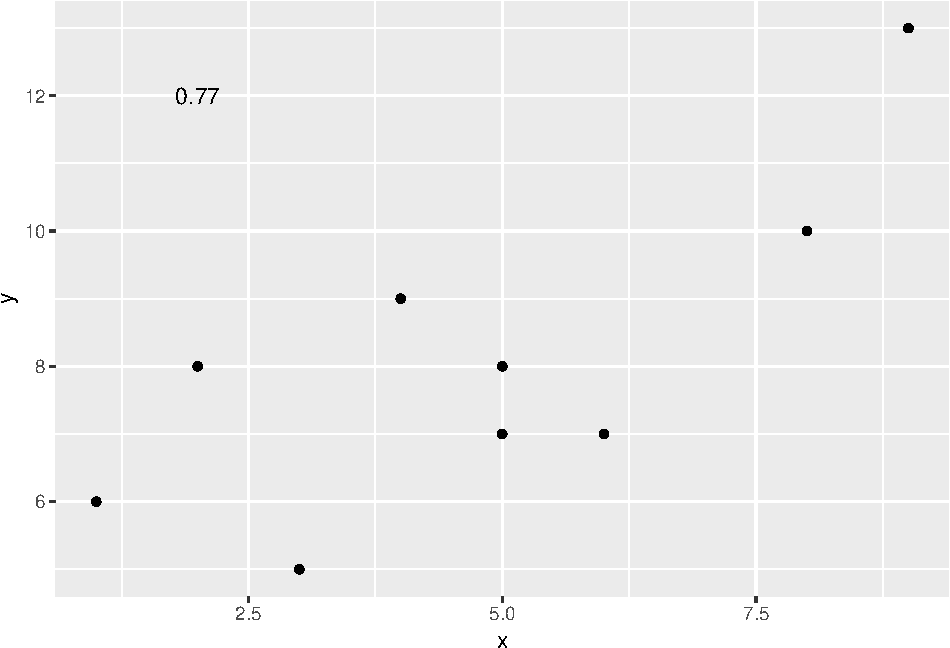
\includegraphics{Programming_Crump_files/figure-latex/unnamed-chunk-77-1.pdf}

Wow, we're moving fast here.

\subsubsection{lots of scatterplots}\label{lots-of-scatterplots}

Before we move on to real data, let's look at some fake data first.
Often we will have many measures of X and Y, split between a few
different conditions, for example, A, B, C, and D. Let's make some fake
data for X and Y, for each condition A, B, C, and D, and then use
facet\_wrapping to look at four scatter plots all at once

\begin{Shaded}
\begin{Highlighting}[]
\NormalTok{x<-}\KeywordTok{rnorm}\NormalTok{(}\DecValTok{40}\NormalTok{,}\DecValTok{0}\NormalTok{,}\DecValTok{1}\NormalTok{)}
\NormalTok{y<-}\KeywordTok{rnorm}\NormalTok{(}\DecValTok{40}\NormalTok{,}\DecValTok{0}\NormalTok{,}\DecValTok{1}\NormalTok{)}
\NormalTok{conditions<-}\KeywordTok{rep}\NormalTok{(}\KeywordTok{c}\NormalTok{(}\StringTok{"A"}\NormalTok{,}\StringTok{"B"}\NormalTok{,}\StringTok{"C"}\NormalTok{,}\StringTok{"D"}\NormalTok{), }\DataTypeTok{each=}\DecValTok{10}\NormalTok{)}

\NormalTok{all_df <-}\StringTok{ }\KeywordTok{data.frame}\NormalTok{(conditions, x, y)}

\KeywordTok{ggplot}\NormalTok{(all_df, }\KeywordTok{aes}\NormalTok{(}\DataTypeTok{x=}\NormalTok{x,}\DataTypeTok{y=}\NormalTok{y))+}
\StringTok{  }\KeywordTok{geom_point}\NormalTok{()+}
\StringTok{  }\KeywordTok{facet_wrap}\NormalTok{(~conditions)}
\end{Highlighting}
\end{Shaded}

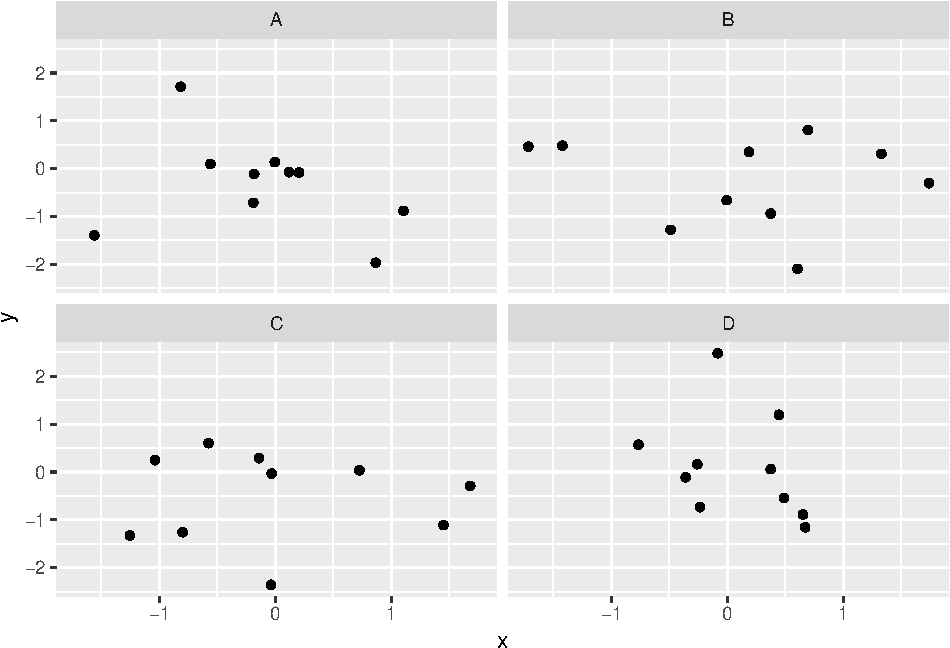
\includegraphics{Programming_Crump_files/figure-latex/unnamed-chunk-78-1.pdf}

\subsubsection{computing the correlations all at
once}\label{computing-the-correlations-all-at-once}

We've seen how we can make four graphs at once. Facet\_wrap will always
try to make as many graphs as there are individual conditions in the
column variable. In this case there are four, so it makes four.

Notice, the scatter plots don't show the correlation (r) values. Getting
these numbers on there is possible, but we have to calculate them first.
We'll leave it to you to Google how to do this, if it's something you
want to do. Instead, what we will do is make a table of the correlations
in addition to the scatter plot. We again use \texttt{dplyr} to do this:

OK, we are basically ready to turn to some real data and ask if there
are correlations between interesting variables\ldots{}You will find that
there are some\ldots{} But before we do that, we do one more thing. This
will help you become a little bit more skeptical of these
``correlations''.

\subsubsection{Chance correlations}\label{chance-correlations}

As you learned from the textbook. We can find correlations by chance
alone, even when there is no true correlation between the variables. For
example, if we sampled randomly into x, and then sampled some numbers
randomly into y. We know they aren't related, because we randomly
sampled the numbers. However, doing this creates some correlations some
of the time just by chance. You can demonstrate this to yourself with
the following code. It's a repeat of what we already saw, jut with a few
more conditions added. Let's look at 20 conditions, with random numbers
for x and y in each. For each, sample size will be 10. We'll make the
fake data, then make a big graph to look at all. And, even though we get
to regression later in the lab, I'll put the best fit line onto each
scatter plot, so you can ``see the correlations''.

\begin{Shaded}
\begin{Highlighting}[]
\NormalTok{x<-}\KeywordTok{rnorm}\NormalTok{(}\DecValTok{10}\NormalTok{*}\DecValTok{20}\NormalTok{,}\DecValTok{0}\NormalTok{,}\DecValTok{1}\NormalTok{)}
\NormalTok{y<-}\KeywordTok{rnorm}\NormalTok{(}\DecValTok{10}\NormalTok{*}\DecValTok{20}\NormalTok{,}\DecValTok{0}\NormalTok{,}\DecValTok{1}\NormalTok{)}
\NormalTok{conditions<-}\KeywordTok{rep}\NormalTok{(}\DecValTok{1}\NormalTok{:}\DecValTok{20}\NormalTok{, }\DataTypeTok{each=}\DecValTok{10}\NormalTok{)}

\NormalTok{all_df <-}\StringTok{ }\KeywordTok{data.frame}\NormalTok{(conditions, x, y)}

\KeywordTok{ggplot}\NormalTok{(all_df, }\KeywordTok{aes}\NormalTok{(}\DataTypeTok{x=}\NormalTok{x,}\DataTypeTok{y=}\NormalTok{y))+}
\StringTok{  }\KeywordTok{geom_point}\NormalTok{()+}
\StringTok{  }\KeywordTok{geom_smooth}\NormalTok{(}\DataTypeTok{method=}\NormalTok{lm, }\DataTypeTok{se=}\OtherTok{FALSE}\NormalTok{)+}
\StringTok{  }\KeywordTok{facet_wrap}\NormalTok{(~conditions)+}
\StringTok{  }\KeywordTok{theme_classic}\NormalTok{()}
\end{Highlighting}
\end{Shaded}

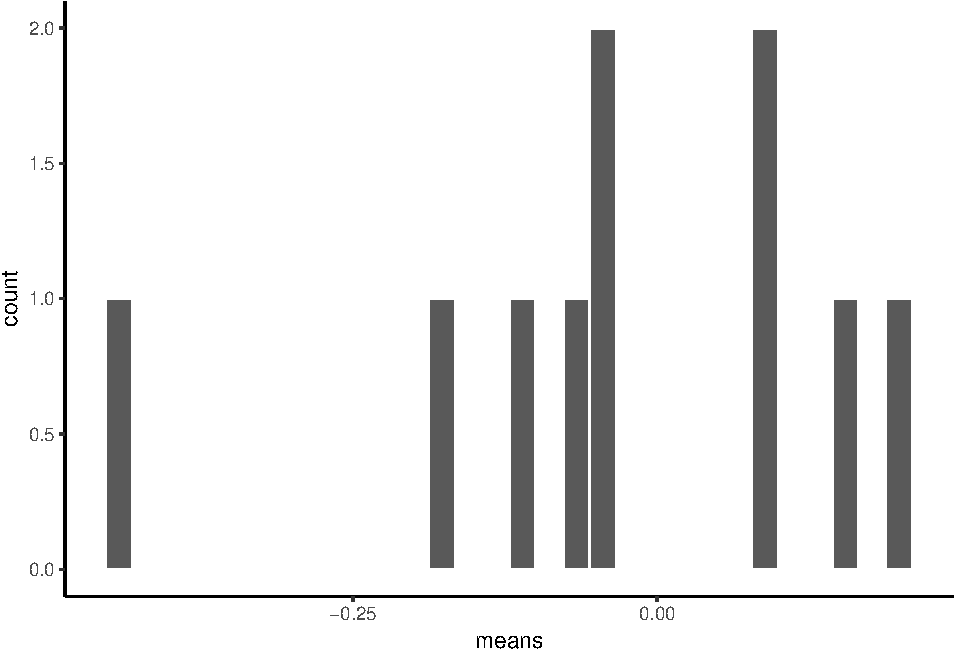
\includegraphics{Programming_Crump_files/figure-latex/unnamed-chunk-79-1.pdf}

You can see that the slope of the blue line is not always flat.
Sometimes it looks like there is a correlation, when we know there
shouldn't be. You can keep re-doing this graph, by re-knitting your R
Markdown document, or by pressing the little green play button. This is
basically you simulating the outcomes as many times as you press the
button.

The point is, now you know you can find correlations by chance. So, in
the next section, you should always wonder if the correlations you find
reflect meaningful association between the x and y variable, or could
have just occurred by chance.

\subsection{Humor Styles
Questionnaire}\label{humor-styles-questionnaire}

Let's take a look at some correlations in real data. We are going to
look at responses to a questionnaire about happiness that was sent
around the world, from the \href{http://worldhappiness.report}{world
happiness report}

\subsubsection{Load the data}\label{load-the-data}

we load the data into a data frame.

\begin{Shaded}
\begin{Highlighting}[]
\KeywordTok{library}\NormalTok{(data.table)}
\NormalTok{whr_data <-}\StringTok{ }\KeywordTok{fread}\NormalTok{(}\StringTok{'data/WHR2018.csv'}\NormalTok{)}
\end{Highlighting}
\end{Shaded}

\subsubsection{Look at the data}\label{look-at-the-data-1}

\begin{Shaded}
\begin{Highlighting}[]
\KeywordTok{library}\NormalTok{(summarytools)}
\KeywordTok{view}\NormalTok{(}\KeywordTok{dfSummary}\NormalTok{(whr_data))}
\end{Highlighting}
\end{Shaded}

You should be able to see that there is data for many different
countries, across a few different years. There are lots of different
kinds of measures, and each are given a name. I'll show you some
examples of asking questions about correlations with this data, then you
get to ask and answer your own questions.

\subsubsection{My Question \#1}\label{my-question-1}

For the year 2017 only, does a countries measure for ``freedom to make
life choices'' correlate with that countries measure for " Confidence in
national government``?

Let's find out. We calculate the correlation, and then we make the
scatter plot.

\begin{Shaded}
\begin{Highlighting}[]
\KeywordTok{cor}\NormalTok{(whr_data$}\StringTok{`}\DataTypeTok{Freedom to make life choices}\StringTok{`}\NormalTok{,}
    \NormalTok{whr_data$}\StringTok{`}\DataTypeTok{Confidence in national government}\StringTok{`}\NormalTok{)}
\end{Highlighting}
\end{Shaded}

\begin{verbatim}
## [1] NA
\end{verbatim}

\begin{Shaded}
\begin{Highlighting}[]
\KeywordTok{ggplot}\NormalTok{(whr_data, }\KeywordTok{aes}\NormalTok{(}\DataTypeTok{x=}\StringTok{`}\DataTypeTok{Freedom to make life choices}\StringTok{`}\NormalTok{,}
                     \DataTypeTok{y=}\StringTok{`}\DataTypeTok{Confidence in national government}\StringTok{`}\NormalTok{))+}
\StringTok{  }\KeywordTok{geom_point}\NormalTok{()+}
\StringTok{  }\KeywordTok{theme_classic}\NormalTok{()}
\end{Highlighting}
\end{Shaded}

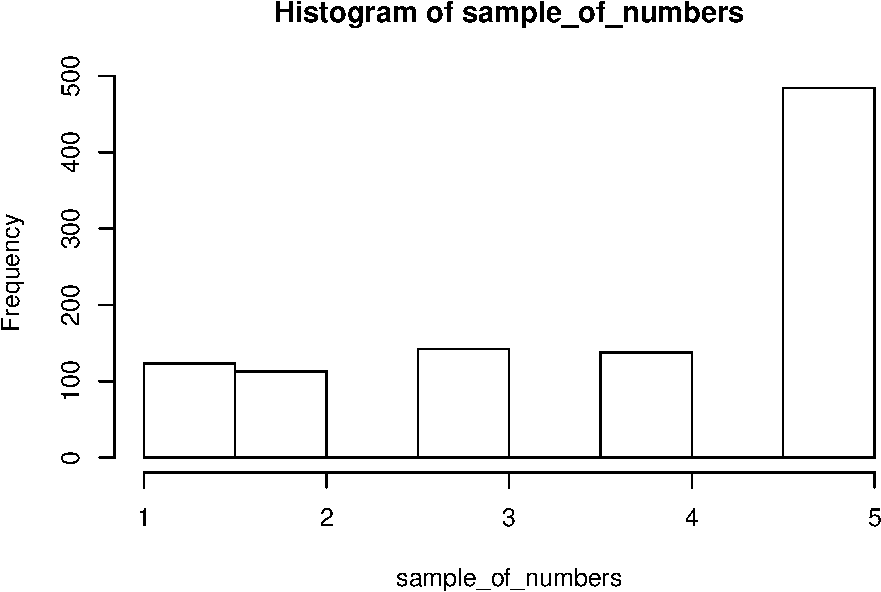
\includegraphics{Programming_Crump_files/figure-latex/unnamed-chunk-82-1.pdf}

Interesting, what happened here? We can see some dots, but the
correlation was NA (meaning undefined). This occurred because there are
some missing data points in the data. We can remove all the rows with
missing data first, then do the correlation. We will do this a couple
steps, first creating our own data.frame with only the numbers we want
to analyse. We can select the columns we want to keep using
\texttt{select}. Then we use \texttt{filter} to remove the rows with
NAs.

\begin{Shaded}
\begin{Highlighting}[]
\KeywordTok{library}\NormalTok{(dplyr)}

\NormalTok{smaller_df <-}\StringTok{ }\NormalTok{whr_data %>%}
\StringTok{               }\KeywordTok{select}\NormalTok{(country,}
                      \StringTok{`}\DataTypeTok{Freedom to make life choices}\StringTok{`}\NormalTok{,}
                      \StringTok{`}\DataTypeTok{Confidence in national government}\StringTok{`}\NormalTok{) %>%}
\StringTok{               }\KeywordTok{filter}\NormalTok{(!}\KeywordTok{is.na}\NormalTok{(}\StringTok{`}\DataTypeTok{Freedom to make life choices}\StringTok{`}\NormalTok{),}
                      \NormalTok{!}\KeywordTok{is.na}\NormalTok{(}\StringTok{`}\DataTypeTok{Confidence in national government}\StringTok{`}\NormalTok{))}

\KeywordTok{cor}\NormalTok{(smaller_df$}\StringTok{`}\DataTypeTok{Freedom to make life choices}\StringTok{`}\NormalTok{,}
    \NormalTok{smaller_df$}\StringTok{`}\DataTypeTok{Confidence in national government}\StringTok{`}\NormalTok{)}
\end{Highlighting}
\end{Shaded}

\begin{verbatim}
## [1] 0.4080963
\end{verbatim}

Now we see the correlation is .408.

Although the scatter plot shows the dots are everywhere, it generally
shows that as Freedom to make life choices increases in a country, that
countries confidence in their national government also increase. This is
a positive correlation. Let's do this again and add the best fit line,
so the trend is more clear, we use
\texttt{geom\_smooth(method=lm,\ se=FALSE)}. I also change the
\texttt{alpha} value of the dots so they blend it bit, and you can see
more of them.

\begin{Shaded}
\begin{Highlighting}[]
\CommentTok{# select DVs and filter for NAs}

\NormalTok{smaller_df <-}\StringTok{ }\NormalTok{whr_data %>%}
\StringTok{               }\KeywordTok{select}\NormalTok{(country,}
                      \StringTok{`}\DataTypeTok{Freedom to make life choices}\StringTok{`}\NormalTok{,}
                      \StringTok{`}\DataTypeTok{Confidence in national government}\StringTok{`}\NormalTok{) %>%}
\StringTok{               }\KeywordTok{filter}\NormalTok{(!}\KeywordTok{is.na}\NormalTok{(}\StringTok{`}\DataTypeTok{Freedom to make life choices}\StringTok{`}\NormalTok{),}
                      \NormalTok{!}\KeywordTok{is.na}\NormalTok{(}\StringTok{`}\DataTypeTok{Confidence in national government}\StringTok{`}\NormalTok{))}

\CommentTok{# calcualte correlation}

\KeywordTok{cor}\NormalTok{(smaller_df$}\StringTok{`}\DataTypeTok{Freedom to make life choices}\StringTok{`}\NormalTok{,}
    \NormalTok{smaller_df$}\StringTok{`}\DataTypeTok{Confidence in national government}\StringTok{`}\NormalTok{)}
\end{Highlighting}
\end{Shaded}

\begin{verbatim}
## [1] 0.4080963
\end{verbatim}

\begin{Shaded}
\begin{Highlighting}[]
\CommentTok{# plot the data with best fit line}

\KeywordTok{ggplot}\NormalTok{(smaller_df, }\KeywordTok{aes}\NormalTok{(}\DataTypeTok{x=}\StringTok{`}\DataTypeTok{Freedom to make life choices}\StringTok{`}\NormalTok{,}
                     \DataTypeTok{y=}\StringTok{`}\DataTypeTok{Confidence in national government}\StringTok{`}\NormalTok{))+}
\StringTok{  }\KeywordTok{geom_point}\NormalTok{(}\DataTypeTok{alpha=}\NormalTok{.}\DecValTok{5}\NormalTok{)+}
\StringTok{  }\KeywordTok{geom_smooth}\NormalTok{(}\DataTypeTok{method=}\NormalTok{lm, }\DataTypeTok{se=}\OtherTok{FALSE}\NormalTok{)+}
\StringTok{  }\KeywordTok{theme_classic}\NormalTok{()}
\end{Highlighting}
\end{Shaded}

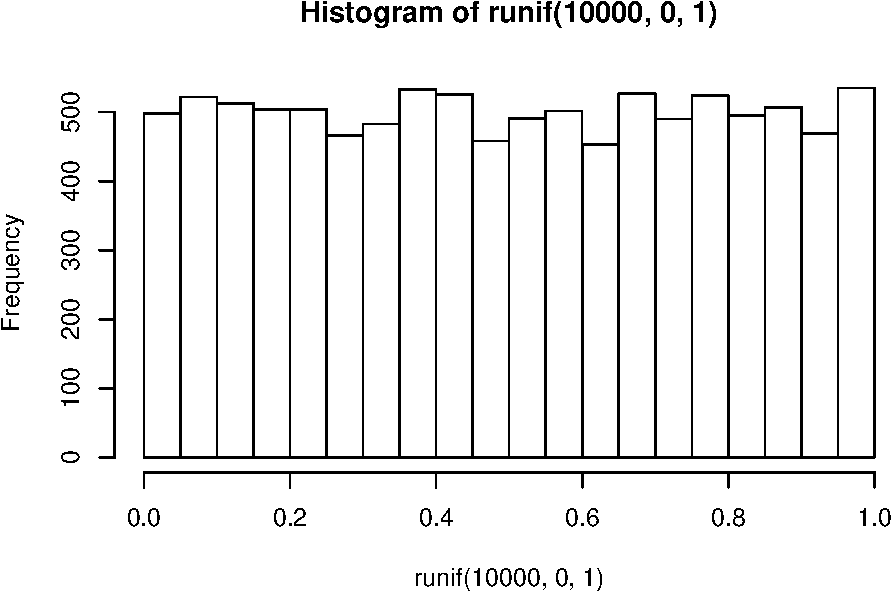
\includegraphics{Programming_Crump_files/figure-latex/unnamed-chunk-84-1.pdf}

\subsubsection{My Question \#2}\label{my-question-2}

After all that work, we can now speedily answer more questions. For
example, what is the relationship between positive affect in a country
and negative affect in a country. I wouldn't be surprised if there was a
negative correlation here: when positive feelings generally go up,
shouldn't negative feelings generally go down?

To answer this question, we just copy paste the last code block, and
change the DVs to be \texttt{Positive\ affect}, and
\texttt{Negative\ affect}

\begin{Shaded}
\begin{Highlighting}[]
\CommentTok{# select DVs and filter for NAs}

\NormalTok{smaller_df <-}\StringTok{ }\NormalTok{whr_data %>%}
\StringTok{               }\KeywordTok{select}\NormalTok{(country,}
                      \StringTok{`}\DataTypeTok{Positive affect}\StringTok{`}\NormalTok{,}
                      \StringTok{`}\DataTypeTok{Negative affect}\StringTok{`}\NormalTok{) %>%}
\StringTok{               }\KeywordTok{filter}\NormalTok{(!}\KeywordTok{is.na}\NormalTok{(}\StringTok{`}\DataTypeTok{Positive affect}\StringTok{`}\NormalTok{),}
                      \NormalTok{!}\KeywordTok{is.na}\NormalTok{(}\StringTok{`}\DataTypeTok{Negative affect}\StringTok{`}\NormalTok{))}

\CommentTok{# calcualte correlation}

\KeywordTok{cor}\NormalTok{(smaller_df$}\StringTok{`}\DataTypeTok{Positive affect}\StringTok{`}\NormalTok{,}
    \NormalTok{smaller_df$}\StringTok{`}\DataTypeTok{Negative affect}\StringTok{`}\NormalTok{)}
\end{Highlighting}
\end{Shaded}

\begin{verbatim}
## [1] -0.3841123
\end{verbatim}

\begin{Shaded}
\begin{Highlighting}[]
\CommentTok{# plot the data with best fit line}

\KeywordTok{ggplot}\NormalTok{(smaller_df, }\KeywordTok{aes}\NormalTok{(}\DataTypeTok{x=}\StringTok{`}\DataTypeTok{Positive affect}\StringTok{`}\NormalTok{,}
                     \DataTypeTok{y=}\StringTok{`}\DataTypeTok{Negative affect}\StringTok{`}\NormalTok{))+}
\StringTok{  }\KeywordTok{geom_point}\NormalTok{(}\DataTypeTok{alpha=}\NormalTok{.}\DecValTok{5}\NormalTok{)+}
\StringTok{  }\KeywordTok{geom_smooth}\NormalTok{(}\DataTypeTok{method=}\NormalTok{lm, }\DataTypeTok{se=}\OtherTok{FALSE}\NormalTok{)+}
\StringTok{  }\KeywordTok{theme_classic}\NormalTok{()}
\end{Highlighting}
\end{Shaded}

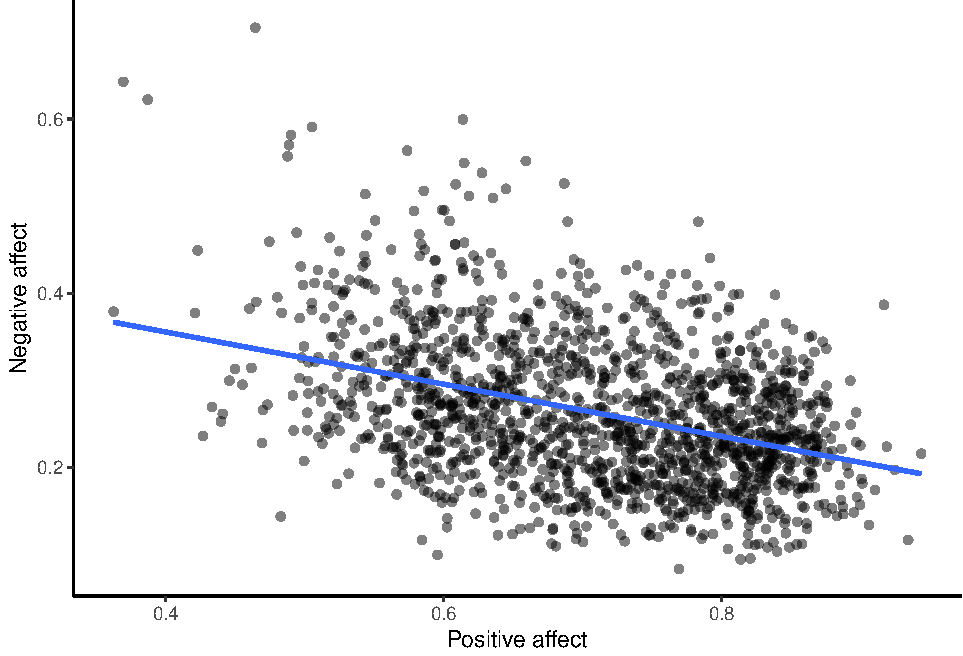
\includegraphics{Programming_Crump_files/figure-latex/unnamed-chunk-85-1.pdf}

Bam, there we have it. As positive affect goes up, negative affect goes
down. A negative correlation.

\subsection{Generalization Exercise}\label{generalization-exercise-1}

Complete the generalization exercise described in your R Markdown
document for this lab.

\subsection{Writing asignment}\label{writing-asignment-1}

Complete the writing assignment described in your R Markdown document
for this lab. When you have finished everything. Knit the document and
hand in your stuff (you can submit your .RMD file to blackboard if it
does not knit.)

\section{Excel}\label{excel-2}

How to do it in Excel

\section{SPSS}\label{spss-2}

How to do it in SPSS

\section{JAMOVI}\label{jamovi-2}

How to do it in JAMOVI

\chapter{Lab 4: Normal Distribution \& Central Limit
Theorem}\label{lab-4-normal-distribution-central-limit-theorem}

{ Some inspiring quote ---Inspiring Person }

\section{Outline of Problem to
solve}\label{outline-of-problem-to-solve-2}

\begin{enumerate}
\def\labelenumi{\arabic{enumi}.}
\tightlist
\item
  Distributions
\item
  Sampling from distributions
\item
  Sampling distribution of the mean
\item
  Sampling statistics (statistics of many samples)
\item
  Central limit theorem
\item
  Normal Distribution
\item
  z-scores
\end{enumerate}

\subsection{important things}\label{important-things-2}

Other things to say

\section{R}\label{r-4}

This is one of two special labs where we don't use too much real data.
We will mostly fake everything. Yes, you will learn how to fake data in
this course. Be a superhero, and only use these skills for good and not
for evil.

As we progress through the course, you will learn how generating
simulated data can be very useful to help you understand real data. In
fact, I will say this right now. If you can't simulate the data you
expect to find, then you probably can't understand the data that you do
find very well. That's a bold statement. It's probably partly true.

\subsection{Generating Numbers in R}\label{generating-numbers-in-r}

There are many ways to make R generate numbers for you. In all of the
case you get define how the numbers are generated. We'll go through a
few of the many ways.

\subsubsection{sample}\label{sample}

The sample function is like an endless gumball machine. You put the
gumballs inside with different properties, say As and Bs, and then you
let sample endlessly take gumballs out. Check it out:

\begin{Shaded}
\begin{Highlighting}[]
\NormalTok{gumballs <-}\StringTok{ }\KeywordTok{c}\NormalTok{(}\StringTok{"A"}\NormalTok{,}\StringTok{"B"}\NormalTok{)}
\NormalTok{sample_of_gumballs <-}\KeywordTok{sample}\NormalTok{(gumballs, }\DecValTok{10}\NormalTok{, }\DataTypeTok{replace=}\OtherTok{TRUE}\NormalTok{)}
\NormalTok{sample_of_gumballs}
\end{Highlighting}
\end{Shaded}

\begin{verbatim}
##  [1] "B" "A" "A" "A" "B" "A" "B" "A" "B" "B"
\end{verbatim}

Here the sample function randomly picks A or B each time. We set it do
this 10 times, so our sample has 10 things in it. We set
\texttt{replace=TRUE} so that after each sample, we put the item back
into the gumball machine and start again. Here's another example with
numbers

\begin{Shaded}
\begin{Highlighting}[]
\NormalTok{some_numbers <-}\StringTok{ }\KeywordTok{c}\NormalTok{(}\DecValTok{1}\NormalTok{,}\DecValTok{2}\NormalTok{,}\DecValTok{3}\NormalTok{,}\DecValTok{4}\NormalTok{,}\DecValTok{5}\NormalTok{,}\DecValTok{5}\NormalTok{,}\DecValTok{5}\NormalTok{,}\DecValTok{5}\NormalTok{)}
\NormalTok{sample_of_numbers <-}\KeywordTok{sample}\NormalTok{(some_numbers, }\DecValTok{20}\NormalTok{, }\DataTypeTok{replace=}\OtherTok{TRUE}\NormalTok{)}
\NormalTok{sample_of_numbers}
\end{Highlighting}
\end{Shaded}

\begin{verbatim}
##  [1] 5 5 2 5 4 5 3 5 5 5 2 2 1 5 5 5 5 5 4 5
\end{verbatim}

Let's do one more thing with sample. Let's sample 1000 times from our
\texttt{some\_numbers} variable, and then look at the histogram

\begin{Shaded}
\begin{Highlighting}[]
\KeywordTok{library}\NormalTok{(ggplot2)}
\NormalTok{some_numbers <-}\StringTok{ }\KeywordTok{c}\NormalTok{(}\DecValTok{1}\NormalTok{,}\DecValTok{2}\NormalTok{,}\DecValTok{3}\NormalTok{,}\DecValTok{4}\NormalTok{,}\DecValTok{5}\NormalTok{,}\DecValTok{5}\NormalTok{,}\DecValTok{5}\NormalTok{,}\DecValTok{5}\NormalTok{)}
\NormalTok{sample_of_numbers <-}\KeywordTok{sample}\NormalTok{(some_numbers, }\DecValTok{1000}\NormalTok{, }\DataTypeTok{replace=}\OtherTok{TRUE}\NormalTok{)}
\KeywordTok{hist}\NormalTok{(sample_of_numbers)}
\end{Highlighting}
\end{Shaded}

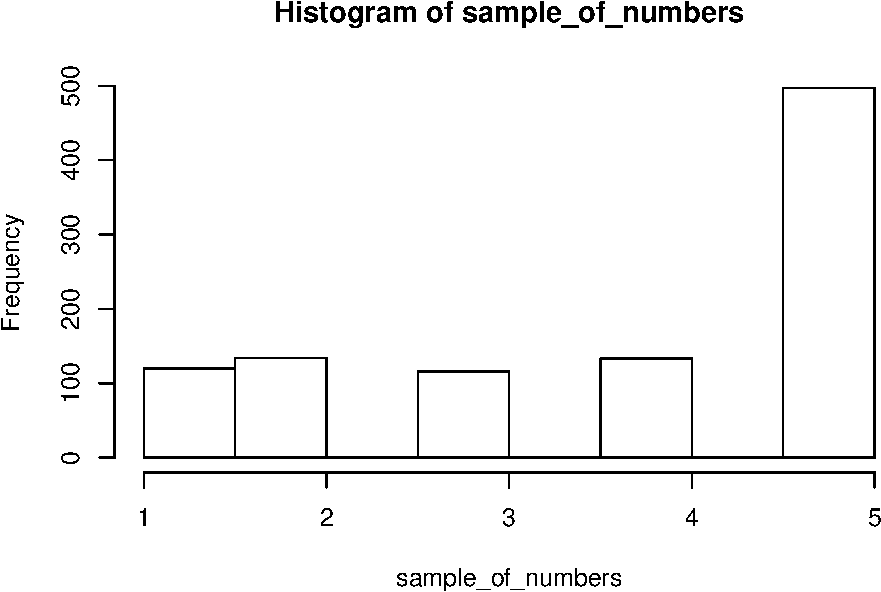
\includegraphics{Programming_Crump_files/figure-latex/unnamed-chunk-88-1.pdf}

We are looking at lots of samples from our little gumball machine of
numbers. We put more 5s in, and voila, more 5s come out of in our big
sample of 1000.

\subsubsection{runif uniform
distribution}\label{runif-uniform-distribution}

We can sample random numbers between any range using the
\texttt{runif(n,\ min=0,\ max\ =\ 1)} function for the uniform
distribution. We discussed this in the textbook. A uniform distribution
is flat, and all the numbers between the min and max should occur
roughly equally frequently. Let's take 1000 random numbers between 0 and
1 and plot the histogram. We'll just do it all in one line for speed.

\begin{Shaded}
\begin{Highlighting}[]
\KeywordTok{hist}\NormalTok{(}\KeywordTok{runif}\NormalTok{(}\DecValTok{1000}\NormalTok{,}\DecValTok{0}\NormalTok{,}\DecValTok{1}\NormalTok{))}
\end{Highlighting}
\end{Shaded}

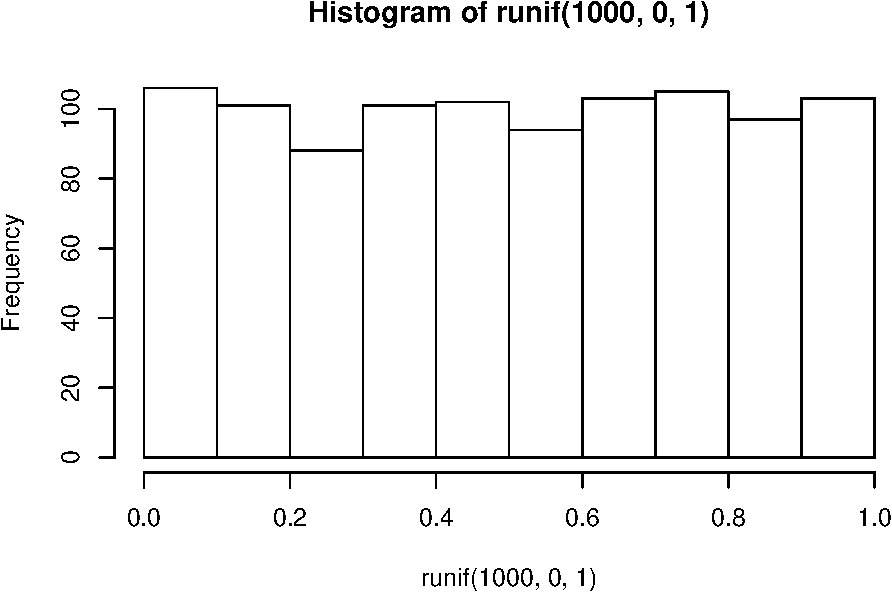
\includegraphics{Programming_Crump_files/figure-latex/unnamed-chunk-89-1.pdf}

This is histogram is flattish. Not perfectly flat, after all we only
took 1000 samples. What if we took many more, say 10,000 total samples?
Now it looks more flat, each bin is occurring about 500 times each,
which is pretty close to the same amount.

\begin{Shaded}
\begin{Highlighting}[]
\KeywordTok{hist}\NormalTok{(}\KeywordTok{runif}\NormalTok{(}\DecValTok{10000}\NormalTok{,}\DecValTok{0}\NormalTok{,}\DecValTok{1}\NormalTok{))}
\end{Highlighting}
\end{Shaded}

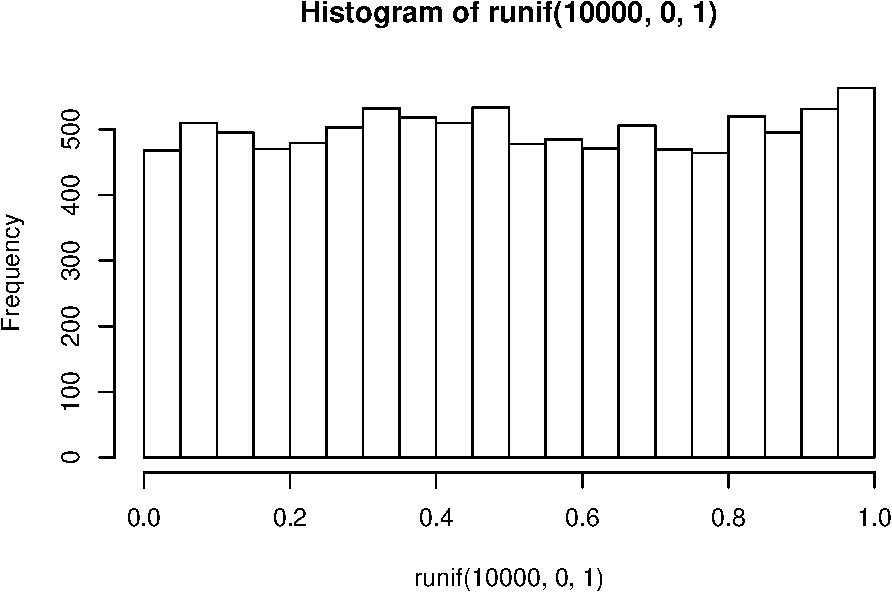
\includegraphics{Programming_Crump_files/figure-latex/unnamed-chunk-90-1.pdf}

\subsubsection{rbinom the binomial
distribution}\label{rbinom-the-binomial-distribution}

The binomial distribution sounds like a scary word\ldots{} binomial
(AAGGGGHHHHH, stay away!). The binomial can be a coin flipping
distribution. You use \texttt{rbinom(n,\ size,\ prob)}. \texttt{n} gives
the number of samples you want to take. We'll keep \texttt{size\ =\ 1}
for now, it's the number of trials (forget this for now, it's more
useful for more complicated things than what we are doing, if you want
to know what it does, try it out, and see if you figure it out).
\texttt{prob} is a little list you make of probabilities, that define
how often certain things happen.

For example, consider flipping a coin. It will be heads or tails, and
the coin, if it is fair, should have a 50\% chance of being heads or
tails. Here's how we flip a coin 10 times using \texttt{rbinom}.

\begin{Shaded}
\begin{Highlighting}[]
\NormalTok{coin_flips <-}\StringTok{ }\KeywordTok{rbinom}\NormalTok{(}\DecValTok{10}\NormalTok{,}\DecValTok{1}\NormalTok{,.}\DecValTok{5}\NormalTok{)}
\NormalTok{coin_flips}
\end{Highlighting}
\end{Shaded}

\begin{verbatim}
##  [1] 0 0 0 1 0 0 1 1 1 0
\end{verbatim}

We get a bunch of 0s, and 1s. We can pretend 0 = tails, and 1 = heads.
Great, now we can do coin flipping if we want. For example, if you flip
10 coins, how many heads do you get? We can can do the above again, and
then \texttt{sum(coin\_flips)}. All the 1s are heads, so it will work
out.

\begin{Shaded}
\begin{Highlighting}[]
\NormalTok{coin_flips <-}\StringTok{ }\KeywordTok{rbinom}\NormalTok{(}\DecValTok{10}\NormalTok{,}\DecValTok{1}\NormalTok{,.}\DecValTok{5}\NormalTok{)}
\KeywordTok{sum}\NormalTok{(coin_flips)}
\end{Highlighting}
\end{Shaded}

\begin{verbatim}
## [1] 6
\end{verbatim}

Alright, so we get the sum, which tells us the number of heads. But,
should we always get that number of heads if we flipped a coin 10 times?
If you keep redoing the above, you'll get different answers. 5 heads
will be the most frequent answer, but you will get lots of other answers
too.

Hold on to your seats for this next one. With R, we can simulate the
flipping of a coin 10 times (you already know that, you just did it),
and we can do that over and over as many times as we want. For example,
we could do it 100 times over, saving the number of heads for each set
of 10 flips. Then we could look at the distribution of those sums. That
would tell us about the range of things that can happen when we flip a
coin 10 times. We can do that in loop like this:

\begin{Shaded}
\begin{Highlighting}[]
\NormalTok{save_number_of_heads<-}\KeywordTok{length}\NormalTok{(}\DecValTok{1000}\NormalTok{) }\CommentTok{# make an empty variable to save things in}

\NormalTok{for(i in }\DecValTok{1}\NormalTok{:}\DecValTok{1000}\NormalTok{)\{}
  \NormalTok{save_number_of_heads[i] <-}\StringTok{ }\KeywordTok{sum}\NormalTok{(}\KeywordTok{rbinom}\NormalTok{(}\DecValTok{10}\NormalTok{,}\DecValTok{1}\NormalTok{,.}\DecValTok{5}\NormalTok{))}
\NormalTok{\}}

\KeywordTok{hist}\NormalTok{(save_number_of_heads)}
\end{Highlighting}
\end{Shaded}

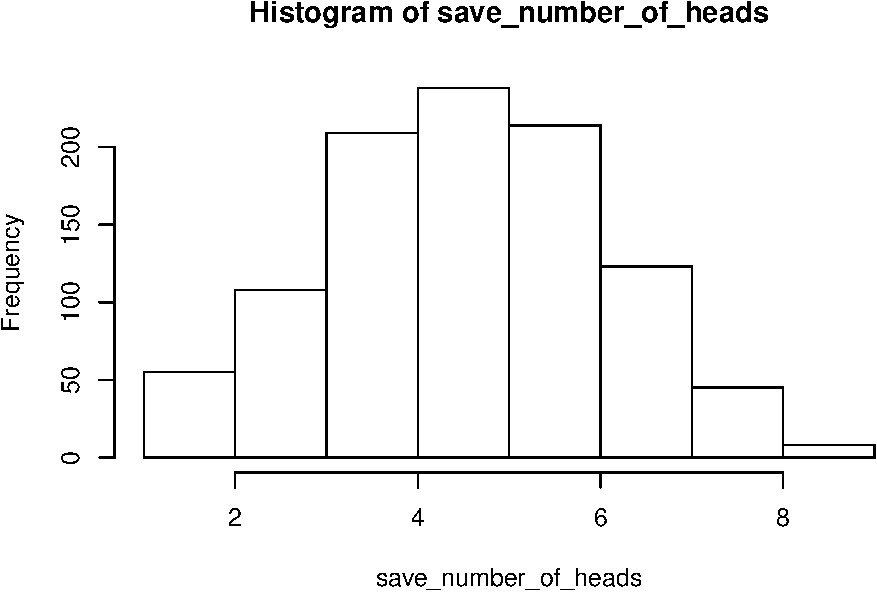
\includegraphics{Programming_Crump_files/figure-latex/unnamed-chunk-93-1.pdf}

See, that wasn't too painful. Now we see another histogram. The
histogram shows us the frequency observing different numbers of heads
(for 10 flips) across the 1000 simulations. 5 happens the most, but 2
happens sometimes, and so does 8. All of the possibilities seem to
happen sometimes, some more than others.

\subsubsection{rnorm the normal
distribution}\label{rnorm-the-normal-distribution}

We'll quickly show how to use \texttt{rnorm(n,\ mean=0,\ sd=1)} to
sample numbers from a normal distribution. And, then we'll come back to
the normal distribution later, because it is so important.

\begin{Shaded}
\begin{Highlighting}[]
\KeywordTok{hist}\NormalTok{(}\KeywordTok{rnorm}\NormalTok{(}\DecValTok{10000}\NormalTok{,}\DecValTok{0}\NormalTok{,}\DecValTok{1}\NormalTok{))}
\end{Highlighting}
\end{Shaded}

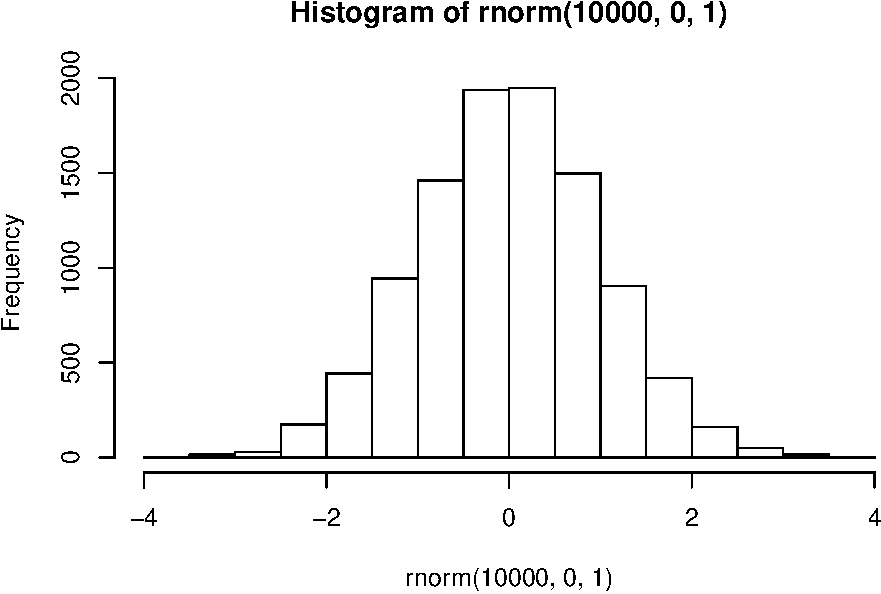
\includegraphics{Programming_Crump_files/figure-latex/unnamed-chunk-94-1.pdf}

There it is, a bell-shaped normal distribution with a mean of 0, and a
standard deviation of 1. You've probably seen things like this before.
Now you can sample numbers from normal distributions with any mean or
standard deviation, just by changing those parts of the \texttt{rnorm}
function.

\subsubsection{mixing it up}\label{mixing-it-up}

The r functions are like Legos, you can put them together and come up
with different things. What if wanted to sample from a distribution that
looked like a two-humped camel's back? Just sample from \texttt{rnorm}
twice like this\ldots{} mix away.

\begin{Shaded}
\begin{Highlighting}[]
\KeywordTok{hist}\NormalTok{( }\KeywordTok{c}\NormalTok{( }\KeywordTok{rnorm}\NormalTok{(}\DecValTok{100}\NormalTok{,}\DecValTok{25}\NormalTok{,}\DecValTok{5}\NormalTok{), }\KeywordTok{rnorm}\NormalTok{(}\DecValTok{100}\NormalTok{,}\DecValTok{50}\NormalTok{,}\DecValTok{5}\NormalTok{)) )}
\end{Highlighting}
\end{Shaded}

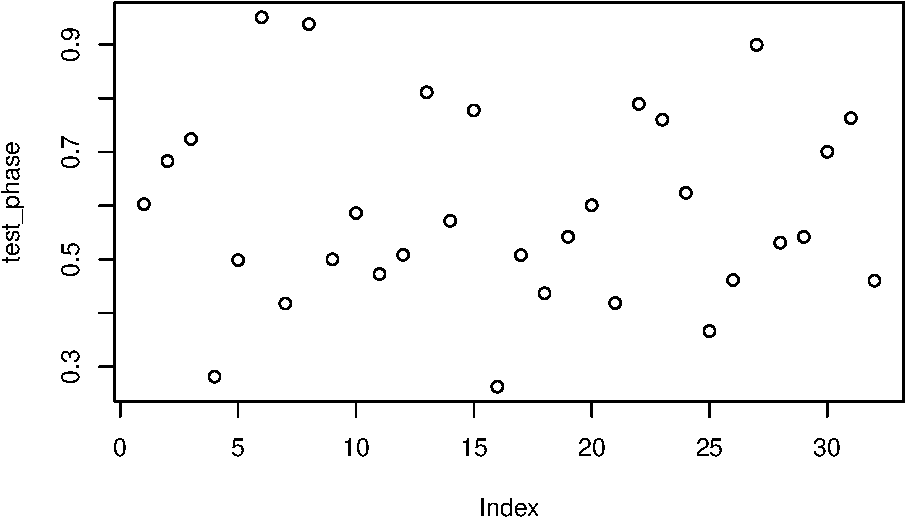
\includegraphics{Programming_Crump_files/figure-latex/unnamed-chunk-95-1.pdf}

\subsubsection{summary}\label{summary}

You can generate as many numbers as your computer can handle with R.
PSA: Don't ask R to generate a bajillion numbers or it will explode (or
more likely just crash, probably won't explode, that's a metaphor).

\subsection{sampling distribution of the
mean.}\label{sampling-distribution-of-the-mean.}

Remember the sampling distribution of the sample means from the
textbook? Now, you will see the R code that made the graphs from before.
As we've seen, we can take samples from distributions in R. We can take
as many as we want. We can set our sample-size to be anything we want.
And, we can take multiple samples of the same size as many times as we
want.

\subsubsection{Taking multiple samples of the same
size}\label{taking-multiple-samples-of-the-same-size}

Let's take 10 samples from a normal distribution (mean = 0, and SD = 1).
Let's set the sample-size for each to be 20. Then, we'll put them all in
a data frame and look at 10 different histograms, one for each sample.

\begin{Shaded}
\begin{Highlighting}[]
\NormalTok{scores <-}\StringTok{ }\KeywordTok{rnorm}\NormalTok{(}\DecValTok{10}\NormalTok{*}\DecValTok{20}\NormalTok{,}\DecValTok{0}\NormalTok{,}\DecValTok{1}\NormalTok{)}
\NormalTok{samples <-}\StringTok{ }\KeywordTok{rep}\NormalTok{(}\DecValTok{1}\NormalTok{:}\DecValTok{10}\NormalTok{,}\DataTypeTok{each=}\DecValTok{20}\NormalTok{)}
\NormalTok{my_df <-}\StringTok{ }\KeywordTok{data.frame}\NormalTok{(samples,scores)}
\end{Highlighting}
\end{Shaded}

First, look at the new my\_df data frame. You can see there is a column
with numbers 1 to 10, these are the sample names. There are also 20
scores for each in the scores column. Let's make histograms for each
sample, so we can see what all of the samples look like:

\begin{Shaded}
\begin{Highlighting}[]
\KeywordTok{ggplot}\NormalTok{(my_df, }\KeywordTok{aes}\NormalTok{(}\DataTypeTok{x=}\NormalTok{scores))+}
\StringTok{  }\KeywordTok{geom_histogram}\NormalTok{(}\DataTypeTok{color=}\StringTok{"white"}\NormalTok{)+}
\StringTok{  }\KeywordTok{facet_wrap}\NormalTok{(~samples)+}
\StringTok{  }\KeywordTok{theme_classic}\NormalTok{()}
\end{Highlighting}
\end{Shaded}

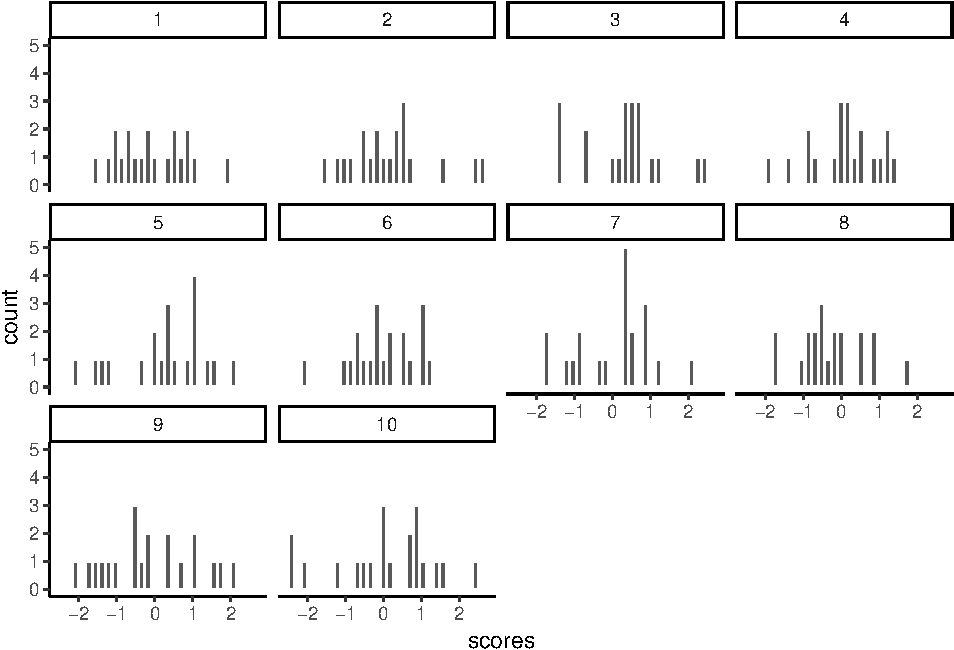
\includegraphics{Programming_Crump_files/figure-latex/unnamed-chunk-97-1.pdf}

Notice, all of the samples do not have the same looking histogram. This
is because of random sampling error. All of the samples are coming from
the same normal distributions, but random chance makes each sample a
little bit different (e.g., you don't always get 5 heads and 5 tails
when you flip a coin right)

\subsubsection{Getting the means of the
samples}\label{getting-the-means-of-the-samples}

Now, let's look at the means of the samples, we will use \texttt{dplyr}
to get the means for each sample, and put them in a table:

\begin{Shaded}
\begin{Highlighting}[]
\KeywordTok{library}\NormalTok{(dplyr)}

\NormalTok{sample_means <-}\StringTok{ }\NormalTok{my_df %>%}
\StringTok{                }\KeywordTok{group_by}\NormalTok{(samples) %>%}
\StringTok{                }\KeywordTok{summarise}\NormalTok{(}\DataTypeTok{means=}\KeywordTok{mean}\NormalTok{(scores))}

\NormalTok{knitr::}\KeywordTok{kable}\NormalTok{(sample_means)}
\end{Highlighting}
\end{Shaded}

\begin{tabular}{r|r}
\hline
samples & means\\
\hline
1 & -0.0736481\\
\hline
2 & 0.1759426\\
\hline
3 & 0.3238048\\
\hline
4 & 0.0977153\\
\hline
5 & 0.2449510\\
\hline
6 & -0.0084961\\
\hline
7 & 0.0160611\\
\hline
8 & -0.2729770\\
\hline
9 & -0.1153894\\
\hline
10 & 0.0382659\\
\hline
\end{tabular}

So, those are the means of our samples. What should the means be? Well,
we would hope they are estimating the mean of the distribution they came
from, which was 0. Notice, the numbers are all not 0, but they are kind
of close to 0.

\#\#\#\# histogram for the means of the samples

What if we now plot these 10 means (of each of the samples) in their own
distribution?

\begin{Shaded}
\begin{Highlighting}[]
 \KeywordTok{ggplot}\NormalTok{(sample_means, }\KeywordTok{aes}\NormalTok{(}\DataTypeTok{x=}\NormalTok{means))+}
\StringTok{  }\KeywordTok{geom_histogram}\NormalTok{(}\DataTypeTok{color=}\StringTok{"white"}\NormalTok{)+}
\StringTok{  }\KeywordTok{theme_classic}\NormalTok{()}
\end{Highlighting}
\end{Shaded}

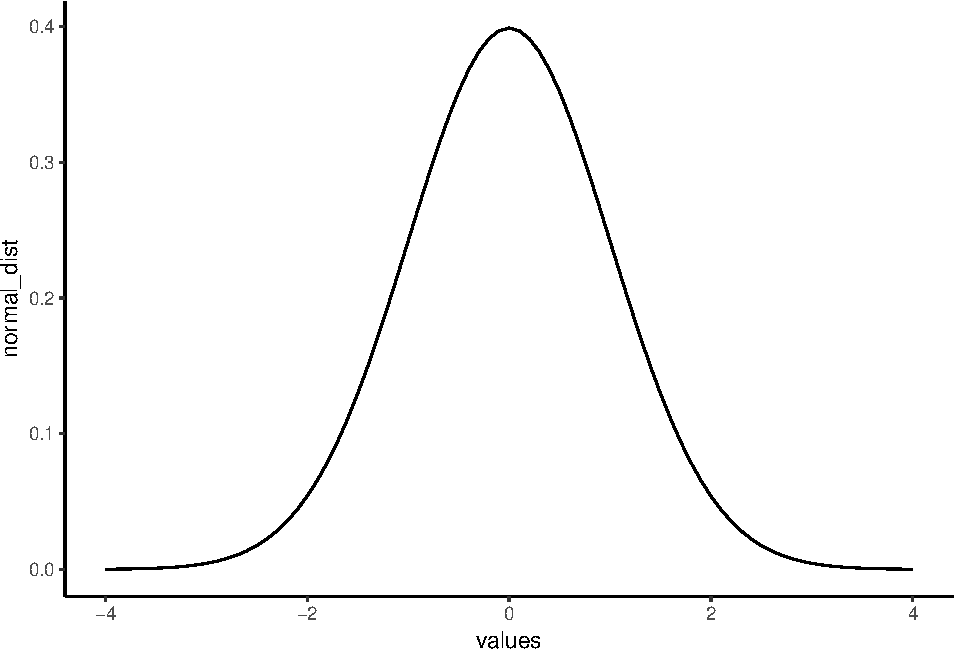
\includegraphics{Programming_Crump_files/figure-latex/unnamed-chunk-99-1.pdf}

That is the distribution of the sample means. It doesn't look like much
eh? That's because we only took 10 samples right.

Notice one more thing\ldots{}What is the mean of our 10 sample means?
This is a mean of means. Remember that.

\begin{Shaded}
\begin{Highlighting}[]
\KeywordTok{mean}\NormalTok{(sample_means$means)}
\end{Highlighting}
\end{Shaded}

\begin{verbatim}
## [1] 0.04262301
\end{verbatim}

Well, that's pretty close to zero. Which is good. When we average over
our samples, they better estimate the mean of the distribution they came
from.

\subsubsection{simulating the distribution of sample
means}\label{simulating-the-distribution-of-sample-means}

Our histogram with 10 sample means looked kind of sad. Let's give it
some more friends. How about we repeat our little sampling experiment
1000 times.

Explain\ldots{}We take 1000 samples. Each sample takes 20 scores from a
normal distribution (mean=0, SD=1). Then we find the means of each
sample (giving us 1000 sample means). Then, we plot that distribution.

\begin{Shaded}
\begin{Highlighting}[]
\CommentTok{# get 1000 samples with 20 scores each}

\NormalTok{scores <-}\StringTok{ }\KeywordTok{rnorm}\NormalTok{(}\DecValTok{1000}\NormalTok{*}\DecValTok{20}\NormalTok{,}\DecValTok{0}\NormalTok{,}\DecValTok{1}\NormalTok{)}
\NormalTok{samples <-}\StringTok{ }\KeywordTok{rep}\NormalTok{(}\DecValTok{1}\NormalTok{:}\DecValTok{1000}\NormalTok{,}\DataTypeTok{each=}\DecValTok{20}\NormalTok{)}
\NormalTok{my_df <-}\StringTok{ }\KeywordTok{data.frame}\NormalTok{(samples,scores)}

\CommentTok{# get the means of the samples}

\NormalTok{sample_means <-}\StringTok{ }\NormalTok{my_df %>%}
\StringTok{                }\KeywordTok{group_by}\NormalTok{(samples) %>%}
\StringTok{                }\KeywordTok{summarise}\NormalTok{(}\DataTypeTok{means=}\KeywordTok{mean}\NormalTok{(scores))}

\CommentTok{# make a histogram}

 \KeywordTok{ggplot}\NormalTok{(sample_means, }\KeywordTok{aes}\NormalTok{(}\DataTypeTok{x=}\NormalTok{means))+}
\StringTok{  }\KeywordTok{geom_histogram}\NormalTok{(}\DataTypeTok{color=}\StringTok{"white"}\NormalTok{)+}
\StringTok{  }\KeywordTok{theme_classic}\NormalTok{()}
\end{Highlighting}
\end{Shaded}

\includegraphics{Programming_Crump_files/figure-latex/unnamed-chunk-101-1.pdf}

There, that looks more like a sampling distribution of the sample means.
Notice it's properties. It is centered on 0, which tells us that sample
means are mostly around zero. It is also bell-shaped, like the normal
distribution it came from. It is also quite narrow. The numbers on the
x-axis don't go much past -.5 to +.5.

We will use things like the sampling distribution of the mean to make
inferences about what chance can do in your data later on in this
course.

\subsection{Sampling distributions for any
statistic}\label{sampling-distributions-for-any-statistic}

Just for fun here are some different sampling distributions for
different statistics. We will take a normal distribution with mean =
100, and standard deviation =20. Then, we'll take lots of samples with n
= 50 (50 observations per sample). We'll save all of the sample
statistics, then plot their histograms. We do the sample means, standard
deviations, maximum values, and medians. Let's do it.

\begin{Shaded}
\begin{Highlighting}[]
\NormalTok{all_df<-}\KeywordTok{data.frame}\NormalTok{()}
\NormalTok{for(i in }\DecValTok{1}\NormalTok{:}\DecValTok{1000}\NormalTok{)\{}
  \NormalTok{sample<-}\KeywordTok{rnorm}\NormalTok{(}\DecValTok{50}\NormalTok{,}\DecValTok{100}\NormalTok{,}\DecValTok{20}\NormalTok{)}
  \NormalTok{sample_mean<-}\KeywordTok{mean}\NormalTok{(sample)}
  \NormalTok{sample_sd<-}\KeywordTok{sd}\NormalTok{(sample)}
  \NormalTok{sample_max<-}\KeywordTok{max}\NormalTok{(sample)}
  \NormalTok{sample_median<-}\KeywordTok{median}\NormalTok{(sample)}
  \NormalTok{t_df<-}\KeywordTok{data.frame}\NormalTok{(i,sample_mean,sample_sd,sample_max,sample_median)}
  \NormalTok{all_df<-}\KeywordTok{rbind}\NormalTok{(all_df,t_df)}
\NormalTok{\}}

\KeywordTok{library}\NormalTok{(ggpubr)}
\NormalTok{a<-}\KeywordTok{ggplot}\NormalTok{(all_df,}\KeywordTok{aes}\NormalTok{(}\DataTypeTok{x=}\NormalTok{sample_mean))+}
\StringTok{  }\KeywordTok{geom_histogram}\NormalTok{(}\DataTypeTok{color=}\StringTok{"white"}\NormalTok{)+}
\StringTok{  }\KeywordTok{theme_classic}\NormalTok{()}
\NormalTok{b<-}\KeywordTok{ggplot}\NormalTok{(all_df,}\KeywordTok{aes}\NormalTok{(}\DataTypeTok{x=}\NormalTok{sample_sd))+}
\StringTok{  }\KeywordTok{geom_histogram}\NormalTok{(}\DataTypeTok{color=}\StringTok{"white"}\NormalTok{)+}
\StringTok{  }\KeywordTok{theme_classic}\NormalTok{()}
\NormalTok{c<-}\KeywordTok{ggplot}\NormalTok{(all_df,}\KeywordTok{aes}\NormalTok{(}\DataTypeTok{x=}\NormalTok{sample_max))+}
\StringTok{  }\KeywordTok{geom_histogram}\NormalTok{(}\DataTypeTok{color=}\StringTok{"white"}\NormalTok{)+}
\StringTok{  }\KeywordTok{theme_classic}\NormalTok{()}
\NormalTok{d<-}\KeywordTok{ggplot}\NormalTok{(all_df,}\KeywordTok{aes}\NormalTok{(}\DataTypeTok{x=}\NormalTok{sample_median))+}
\StringTok{  }\KeywordTok{geom_histogram}\NormalTok{(}\DataTypeTok{color=}\StringTok{"white"}\NormalTok{)+}
\StringTok{  }\KeywordTok{theme_classic}\NormalTok{()}

\KeywordTok{ggarrange}\NormalTok{(a,b,c,d,}
          \DataTypeTok{ncol =} \DecValTok{2}\NormalTok{, }\DataTypeTok{nrow =} \DecValTok{2}\NormalTok{)}
\end{Highlighting}
\end{Shaded}

\includegraphics{Programming_Crump_files/figure-latex/unnamed-chunk-102-1.pdf}

From reading the textbook and attending lecture, you should be able to
start thinking about why these sampling statistic distributions might be
useful\ldots{}For now, just know that you can make a sampling statistic
for pretty much anything in R, just by simulating the process of
sampling, measuring the statistic, doing it over a bunch, and then
plotting the histogram. This gives you a pretty good estimate of the
distribution for that sampling statistic.

\subsection{Central limit theorem}\label{central-limit-theorem}

We have been building you up for the central limit theorem, described in
the textbook and in class. The central limit theorem is basically that
the distribution of sample means will be a normal curve. We already saw
that before. But, the interesting thing about it, is that the
distribution of your sample means will be normal, even if the
distribution the samples came from is not normal. Huh what?

To demonstrate this the next bit of code is modified from what we did
earlier. We create 100 samples. Each sample has 1000 observations. All
of them come from a uniform distribution between 0 to 1. This means all
of the numbers between 0 and 1 should occur equally frequently. Below I
plot histograms for the first 10 samples (out of the 100 total, 100 is
too many to look at). Notice the histograms are not normal, they are
roughly flat.

\begin{Shaded}
\begin{Highlighting}[]
\NormalTok{scores <-}\StringTok{ }\KeywordTok{runif}\NormalTok{(}\DecValTok{100}\NormalTok{*}\DecValTok{1000}\NormalTok{,}\DecValTok{0}\NormalTok{,}\DecValTok{1}\NormalTok{)}
\NormalTok{samples <-}\StringTok{ }\KeywordTok{rep}\NormalTok{(}\DecValTok{1}\NormalTok{:}\DecValTok{100}\NormalTok{,}\DataTypeTok{each=}\DecValTok{1000}\NormalTok{)}
\NormalTok{my_df <-}\StringTok{ }\KeywordTok{data.frame}\NormalTok{(samples,scores)}

\KeywordTok{ggplot}\NormalTok{(my_df[}\DecValTok{1}\NormalTok{:(}\DecValTok{10}\NormalTok{*}\DecValTok{1000}\NormalTok{),], }\KeywordTok{aes}\NormalTok{(}\DataTypeTok{x=}\NormalTok{scores))+}
\StringTok{  }\KeywordTok{geom_histogram}\NormalTok{(}\DataTypeTok{color=}\StringTok{"white"}\NormalTok{, }\DataTypeTok{bins=}\DecValTok{10}\NormalTok{)+}
\StringTok{  }\KeywordTok{facet_wrap}\NormalTok{(~samples)+}
\StringTok{  }\KeywordTok{theme_classic}\NormalTok{()+}
\StringTok{  }\KeywordTok{ylim}\NormalTok{(}\DecValTok{0}\NormalTok{,}\DecValTok{200}\NormalTok{)}
\end{Highlighting}
\end{Shaded}

\includegraphics{Programming_Crump_files/figure-latex/unnamed-chunk-103-1.pdf}

We took samples from a flat uniform distribution, and the samples
themselves look like that same flat distribution.

HOWEVER, if we now do the next step, and compute the means of each of
our 100 samples, we could then look at the sampling distribution of the
sample means. Let's do that:

\begin{Shaded}
\begin{Highlighting}[]
\NormalTok{sample_means <-}\StringTok{ }\NormalTok{my_df %>%}
\StringTok{                }\KeywordTok{group_by}\NormalTok{(samples) %>%}
\StringTok{                }\KeywordTok{summarise}\NormalTok{(}\DataTypeTok{means=}\KeywordTok{mean}\NormalTok{(scores))}

\CommentTok{# make a histogram}

 \KeywordTok{ggplot}\NormalTok{(sample_means, }\KeywordTok{aes}\NormalTok{(}\DataTypeTok{x=}\NormalTok{means))+}
\StringTok{  }\KeywordTok{geom_histogram}\NormalTok{(}\DataTypeTok{color=}\StringTok{"white"}\NormalTok{, }\DataTypeTok{bins=}\DecValTok{15}\NormalTok{)+}
\StringTok{  }\KeywordTok{theme_classic}\NormalTok{()}
\end{Highlighting}
\end{Shaded}

\includegraphics{Programming_Crump_files/figure-latex/unnamed-chunk-104-1.pdf}

As you can see, the sampling distribution of the sample means is not
flat. It's shaped kind of normal-ish. If we had taken many more samples,
found their means, and then looked at a histogram, it would become even
more normal looking. Because that's what happens according to the
central limit theorem.

\subsection{The normal distribution}\label{the-normal-distribution}

``Why does any of this matter, why are we doing this, can we stop
now!!!!!! PLEEEEAASSEE, somebody HELP''.

We are basically just repeating what was said in the textbook, and the
lecture, so that you get the concept explained in a bunch of different
ways. It will sink in.

The reason the central limit theorem is important, is because
researchers often take many samples, then analyse the means of their
samples. That's what they do.

An experiment might have 20 people. You might take 20 measurements from
each person. That's taking 20 samples. Then, because we know that
samples are noisy. We take the means of the samples.

So, what researchers are often looking at, (and you too, very soon) are
means of samples. Not just the samples. And, now we know that means of
samples (if we had a lot of samples), look like they are distributed
normally (the central limit theorem says the should be).

We can use this knowledge. If we learn a little bit more about normal
distributions, and how they behave and work, we can take that and use it
to understand our sample means better. This will become more clear as
head into the topic of statistical inference next week. This is all a
build up for that.

To continue the build-up we now look at some more properties of the
normal distribution.

\subsubsection{Graphing the normal
distribution}\label{graphing-the-normal-distribution}

``Wait, I thought we already did that''. We sort of did. We sampled
numbers and made histograms that looked like normal distributions. But,
a ``normal distribution'' is more of an abstract idea. It looks like
this in the abstract:

\begin{Shaded}
\begin{Highlighting}[]
\NormalTok{normal_dist <-}\StringTok{ }\KeywordTok{dnorm}\NormalTok{(}\KeywordTok{seq}\NormalTok{(-}\DecValTok{4}\NormalTok{,}\DecValTok{4}\NormalTok{,.}\DecValTok{1}\NormalTok{), }\DecValTok{0}\NormalTok{, }\DecValTok{1}\NormalTok{)}
\NormalTok{values <-}\KeywordTok{seq}\NormalTok{(-}\DecValTok{4}\NormalTok{,}\DecValTok{4}\NormalTok{,.}\DecValTok{1}\NormalTok{)}
\NormalTok{normal_df <-}\KeywordTok{data.frame}\NormalTok{(values,normal_dist)}

\KeywordTok{ggplot}\NormalTok{(normal_df, }\KeywordTok{aes}\NormalTok{(}\DataTypeTok{x=}\NormalTok{values,}\DataTypeTok{y=}\NormalTok{normal_dist))+}
\StringTok{  }\KeywordTok{geom_line}\NormalTok{()+}
\StringTok{  }\KeywordTok{theme_classic}\NormalTok{()}
\end{Highlighting}
\end{Shaded}

\includegraphics{Programming_Crump_files/figure-latex/unnamed-chunk-105-1.pdf}

A really nice shaped bell-like thing. This normal distribution has a
mean of 0, and standard deviation of 1. The heights of the lines tell
you roughly how likely each value is. Notice, it is centered on 0 (most
likely that numbers from this distribution will be near 0), and it goes
down as numbers get bigger or smaller (so bigger or smaller numbers get
less likely). There is a range to it. Notice the values don't go much
beyond -4 and +4. This because those values don't happen very often.
Theoretically any value could happen, but really big or small values
have really low probabilities.

\subsubsection{calculating the probability of specific
ranges.}\label{calculating-the-probability-of-specific-ranges.}

We can use R to tell us about the probability of getting numbers in a
certain range. For example, when you think about. It should be obvious
that you have a 50\% probability of getting the number 0 or greater.
Half of the distribution is 0 or greater, so you have a 50\%
probability.

We can use the \texttt{pnorm} function to confirm this:

\begin{Shaded}
\begin{Highlighting}[]
\KeywordTok{pnorm}\NormalTok{(}\DecValTok{0}\NormalTok{, }\DataTypeTok{mean =} \DecValTok{0}\NormalTok{, }\DataTypeTok{sd=} \DecValTok{1}\NormalTok{, }\DataTypeTok{lower.tail=}\OtherTok{FALSE}\NormalTok{)}
\end{Highlighting}
\end{Shaded}

\begin{verbatim}
## [1] 0.5
\end{verbatim}

Agreed, \texttt{pnorm} tells us the probability of getting 0 or greater
is .5.

Well, what is the probability of getting a 2 or greater? That's a bit
harder to judge, obviously less than 50\%. Use R like this to find out:

\begin{Shaded}
\begin{Highlighting}[]
\KeywordTok{pnorm}\NormalTok{(}\DecValTok{2}\NormalTok{, }\DataTypeTok{mean =} \DecValTok{0}\NormalTok{, }\DataTypeTok{sd=} \DecValTok{1}\NormalTok{, }\DataTypeTok{lower.tail=}\OtherTok{FALSE}\NormalTok{)}
\end{Highlighting}
\end{Shaded}

\begin{verbatim}
## [1] 0.02275013
\end{verbatim}

The probability of getting a 2 or greater is .0227 (not very probable)

What is the probability of getting a score between -1 and 1?

\begin{Shaded}
\begin{Highlighting}[]
\NormalTok{ps<-}\KeywordTok{pnorm}\NormalTok{(}\KeywordTok{c}\NormalTok{(-}\DecValTok{1}\NormalTok{,}\DecValTok{1}\NormalTok{), }\DataTypeTok{mean =} \DecValTok{0}\NormalTok{, }\DataTypeTok{sd=} \DecValTok{1}\NormalTok{, }\DataTypeTok{lower.tail=}\OtherTok{FALSE}\NormalTok{)}
\NormalTok{ps[}\DecValTok{1}\NormalTok{]-ps[}\DecValTok{2}\NormalTok{]}
\end{Highlighting}
\end{Shaded}

\begin{verbatim}
## [1] 0.6826895
\end{verbatim}

About 68\%. About 68\% of all the numbers would be between -1 and 1. So
naturally, about 34\% of the numbers would be between 0 and 1. Notice,
we are just getting a feeling for this, you'll see why in a bit when we
do z-scores (some of you may realize we are already doing that\ldots{})

What about the numbers between 1 and 2?

\begin{Shaded}
\begin{Highlighting}[]
\NormalTok{ps<-}\KeywordTok{pnorm}\NormalTok{(}\KeywordTok{c}\NormalTok{(}\DecValTok{1}\NormalTok{,}\DecValTok{2}\NormalTok{), }\DataTypeTok{mean =} \DecValTok{0}\NormalTok{, }\DataTypeTok{sd=} \DecValTok{1}\NormalTok{, }\DataTypeTok{lower.tail=}\OtherTok{FALSE}\NormalTok{)}
\NormalTok{ps[}\DecValTok{1}\NormalTok{]-ps[}\DecValTok{2}\NormalTok{]}
\end{Highlighting}
\end{Shaded}

\begin{verbatim}
## [1] 0.1359051
\end{verbatim}

About 13.5\% of numbers fall in that range, not much.

How about between 2 and 3?

\begin{Shaded}
\begin{Highlighting}[]
\NormalTok{ps<-}\KeywordTok{pnorm}\NormalTok{(}\KeywordTok{c}\NormalTok{(}\DecValTok{2}\NormalTok{,}\DecValTok{3}\NormalTok{), }\DataTypeTok{mean =} \DecValTok{0}\NormalTok{, }\DataTypeTok{sd=} \DecValTok{1}\NormalTok{, }\DataTypeTok{lower.tail=}\OtherTok{FALSE}\NormalTok{)}
\NormalTok{ps[}\DecValTok{1}\NormalTok{]-ps[}\DecValTok{2}\NormalTok{]}
\end{Highlighting}
\end{Shaded}

\begin{verbatim}
## [1] 0.02140023
\end{verbatim}

Again a very small amount, only 2.1 \% of the numbers, not a a lot.

\subsubsection{summary pnorm}\label{summary-pnorm}

You can always use \texttt{pnorm} to figure how the probabilities of
getting certain values from any normal distribution. That's great.

\subsection{z-scores}\label{z-scores}

We just spent a bunch of time looking at a very special normal
distribution, the one where the mean = 0, and the standard deviation =
1. Then we got a little bit comfortable with what those numbers mean. 0
happens a lot. Numbers between -1 and 1 happen a lot. Numbers bigger or
smaller than 1 also happen fairly often, but less often. Number bigger
than 2 don't happen a lot, numbers bigger than 3 don't happen hardly at
all.

We can use this knowledge for our convenience. Often, we are not dealing
with numbers exactly like these. For example, someone might say, I got a
number, it's 550. It came from a distribution with mean = 600, and
standard deviation = 25. So, does 545 happen a lot or not? The numbers
don't tell you right away.

If we were talking about our handy distribution with mean = 0 and
standard deviation = 1, and I told I got a number 4.5 from that
distribution. You would automatically know that 4.5 doesn't happen a
lot. Right? Right!

z-scores are a way of transforming one set of numbers into our neato
normal distribution, with mean = 0 and standard deviation = 1.

Here's a simple example, like what we said in the textbook. If you have
a normal distribution with mean = 550, and standard deviation 25, then
how far from the mean is the number 575? It's a whole 25 away (550+25 =
575). How many standard deviations is that? It's 1 whole standard
deviation. So does a number like 575 happen a lot? Well, based on what
you know about normal distributions, 1 standard deviation of the mean
isn't that far, and it does happen fairly often. This is what we are
doing here.

\subsubsection{Calculating z-scores}\label{calculating-z-scores}

\begin{enumerate}
\def\labelenumi{\arabic{enumi}.}
\tightlist
\item
  get some numbers
\end{enumerate}

\begin{Shaded}
\begin{Highlighting}[]
\NormalTok{some_numbers <-}\StringTok{ }\KeywordTok{rnorm}\NormalTok{(}\DecValTok{20}\NormalTok{,}\DecValTok{50}\NormalTok{,}\DecValTok{25}\NormalTok{)}
\end{Highlighting}
\end{Shaded}

\begin{enumerate}
\def\labelenumi{\arabic{enumi}.}
\setcounter{enumi}{1}
\tightlist
\item
  Calculate the mean and standard deviation
\end{enumerate}

\begin{Shaded}
\begin{Highlighting}[]
\NormalTok{my_mean <-}\StringTok{ }\KeywordTok{mean}\NormalTok{(some_numbers)}
\NormalTok{my_sd <-}\KeywordTok{sd}\NormalTok{(some_numbers)}

\KeywordTok{print}\NormalTok{(my_mean)}
\end{Highlighting}
\end{Shaded}

\begin{verbatim}
## [1] 50.02857
\end{verbatim}

\begin{Shaded}
\begin{Highlighting}[]
\KeywordTok{print}\NormalTok{(my_sd)}
\end{Highlighting}
\end{Shaded}

\begin{verbatim}
## [1] 27.23455
\end{verbatim}

\begin{enumerate}
\def\labelenumi{\arabic{enumi}.}
\setcounter{enumi}{2}
\tightlist
\item
  subtract the mean from your numbers
\end{enumerate}

\begin{Shaded}
\begin{Highlighting}[]
\NormalTok{differences<-some_numbers-my_mean}
\KeywordTok{print}\NormalTok{(my_sd)}
\end{Highlighting}
\end{Shaded}

\begin{verbatim}
## [1] 27.23455
\end{verbatim}

\begin{enumerate}
\def\labelenumi{\arabic{enumi}.}
\setcounter{enumi}{3}
\tightlist
\item
  divide by the standard deviation
\end{enumerate}

\begin{Shaded}
\begin{Highlighting}[]
\NormalTok{z_scores<-differences/my_sd}
\KeywordTok{print}\NormalTok{(z_scores)}
\end{Highlighting}
\end{Shaded}

\begin{verbatim}
##  [1] -0.20011359  1.21876252  0.77224612  0.49107624 -0.59732747
##  [6] -0.39124337  0.14905347 -0.82439512  0.06832726 -1.07170308
## [11] -1.62565408 -0.13210288 -0.80832484 -0.57890065 -0.35931783
## [16]  2.46523045  0.47588190  0.54268971  1.58377947 -1.17796423
\end{verbatim}

Done. Now you have converted your original numbers into what we call
standardized scores. They are standardized to have the same properties
(assumed properties) as a normal distribution with mean = 0, and SD = 1.

You could look at each of your original scores, and try to figure out if
they are likely or unlikely numbers. But, if you make them into
z-scores, then you can tell right away. Numbers close to 0 happen a lot,
bigger numbers closer to 1 happen less often, but still fairly often,
and number bigger than 2 or 3 hardly happen at all.

If someone said they did 3 standard deviations above the mean on a test,
this means they did really good, and hardly nobody also did that good.

Z-scores are a useful language once you understand them. We show you
this language in case you find them useful.

\subsection{Generalization Exercise}\label{generalization-exercise-2}

Complete the generalization exercise described in your R Markdown
document for this lab.

\subsection{Writing asignment}\label{writing-asignment-2}

Complete the writing assignment described in your R Markdown document
for this lab. When you have finished everything. Knit the document and
hand in your stuff (you can submit your .RMD file to blackboard if it
does not knit.)

\section{Excel}\label{excel-3}

How to do it in Excel

\section{SPSS}\label{spss-3}

How to do it in SPSS

\section{JAMOVI}\label{jamovi-3}

How to do it in JAMOVI

\chapter{Lab 5: Fundamentals of Hypothesis
Testing}\label{lab-5-fundamentals-of-hypothesis-testing}

{ Some inspiring quote ---Inspiring Person }

\section{Outline of Problem to
solve}\label{outline-of-problem-to-solve-3}

\subsection{important things}\label{important-things-3}

Other things to say

\section{R}\label{r-5}

From here on out in the labs we will be focusing on making sense of data
from experiments. In all of this, we use experiments to ask a question
about whether one thing causes change (influences) another thing. Then,
we look at the data to help us answer that question. In general, we
expect to find a difference in our measurement between the conditions of
the experimental manipulation. We expect to find a difference when the
manipulation works, and causes change in our measure. We expect not to
find a difference when the manipulation does not work, and does not
cause change.

However, as you well know from reading the textbook, and attending the
lectures. Experimental manipulations are not the only thing that can
cause change in our measure. Chance alone can cause change. Our measures
are usually variable themselves, so they come along with some change in
them due to sampling error.

At a minimum, when we conduct an experiment, we want to know \textbf{if
the change we observed is bigger than the change that can be produced by
chance}. Theoretically, random chance could produce most any change we
might measure in our experiment. So, there will always be uncertainty
about whether our manipulation caused the change, or chance caused the
change. But, we can reduce and evaluate that uncertainty. When we do
this, we make \textbf{inferences} about what caused change in our
experiments. This process is called \textbf{statistical inference}. We
use \textbf{inferential statistics} as tools to help us make these
inferences.

In this lab we introduce you to foundational concepts in
\textbf{statistical inference}. This is also commonly termed
\textbf{hypothesis testing}. But, for various reasons using that
language to describe the process is tied to particular philosophies
about doing statistical inference. We use some of that language here, so
that you know what it means. But, we also use our own plain language, so
you know what the point is, without the statistical jargon.

The textbook describes a few different statistical tests for building
your conceptual understanding for statistical inference. In this lab, we
work through some of them. In particular, we work through the Crump
test, and the Randomization test. We show you how to conduct these tests
in R on fake data, and real data.

\subsection{The Crump Test}\label{the-crump-test}

\href{https://crumplab.github.io/statistics/foundations-for-inference.html\#the-crump-test}{The
Crump test is described more fully in the textbook here}, but you
already read that in preparation for this lab, right! I hope you did.

The big idea behind the Crump test is this. You find out what kind of
differences between two conditions can be found by chance alone. This
shows you what chance can do. Then, you compare what you actually found
in one experiment, with the chance distribution, and make an inference
about whether or not chance could have produced the difference.

\subsubsection{Make assumptions about the distribution for your
measurement}\label{make-assumptions-about-the-distribution-for-your-measurement}

The first step in conducting the Crump test is to make a guess at the
distribution behind your measurement. We will see in the next part how
to do this from real data. For now, we just pick a distribution. For
example, let's say we are measuring something that comes from a normal
distribution with mean = 75 and standard deviation = 5. Perhaps, this is
a distribution for how people perform on a particular test. The mean on
the test is 75\%, with a standard deviation of 5\%. We know from last
lab that 3 standard deviations away from the mean is pretty unlikely
with this distribution. So, for example, most people never score above
90\% (5*3=15, 75+15 = 90) on this test.

In this example situation, we might imagine an experiment that was
conducted to determine whether manipulation A improves test performance,
compared to a control condition where no manipulation took place. Using
the Crump test, we can simulate differences that can occur by chance. We
are formally simulating the differences that could be obtained between
two control conditions, where no manipulation took place.

To, restate our assumptions, we assume a single score for each subject
is sampled from:

\texttt{rnorm(n,\ mean=75,\ sd=5)}

\subsubsection{Make assumptions about N}\label{make-assumptions-about-n}

In the real world, experiments have some number of subjects in each
condition, this number is called N. For our simulation we, need to
choose the number of subjects that we have. For this demonstration, we
choose N = 20 in each condition.

\subsubsection{Choose the number of simulations to
run}\label{choose-the-number-of-simulations-to-run}

We are going to run a fake experiment with no manipulation, and do this
many times over (doing it many times over is called \textbf{monte carlo
simulation}). Each time we will do this:

\begin{enumerate}
\def\labelenumi{\arabic{enumi}.}
\tightlist
\item
  Sample 20 numbers for control group A using
  \texttt{rnorm(20,\ mean=75,\ sd=5)}
\item
  Sample 20 numbers for control group B using
  \texttt{rnorm(20,\ mean=75,\ sd=5)}
\item
  Compute the means for control group A and B
\item
  Compute the difference between the mean for group A and B
\item
  Save the differences score in a variable
\item
  Repeat as many times as we want
\end{enumerate}

If we repeat the simulation 100 times, we will see the differences that
can be produced by chance, when given the opportunity 100 times. For
example, in a simulation like this, the biggest difference (the maximum
value) only happens once. We can find that difference, and then roughly
conclude that a difference of that big happens 1 out of 100 times just
by chance. That's not a lot.

If we want to be more restrictive, we can make the simulation go to
1,000, or 10,000, or greater. Each time the maximum value will tell us
what is the biggest thing chance did 1 out of 1000 times, or 1 out of
10,000 times.

The textbook uses 10,000 times. Let's use 100 times here to keep things
simple.

\subsubsection{Run the simluation}\label{run-the-simluation}

\begin{Shaded}
\begin{Highlighting}[]
\KeywordTok{library}\NormalTok{(ggplot2)}

\CommentTok{# set paramaters of simulation}

\NormalTok{sims_to_run <-}\StringTok{ }\DecValTok{100}
\NormalTok{sample_n   <-}\StringTok{ }\DecValTok{20}
\NormalTok{dist_mean  <-}\StringTok{ }\DecValTok{75}
\NormalTok{dist_sd    <-}\StringTok{ }\DecValTok{5}

\CommentTok{# run simulation}

\NormalTok{mean_differences <-}\StringTok{ }\KeywordTok{length}\NormalTok{(sims_to_run)}
\NormalTok{for(i in }\DecValTok{1}\NormalTok{:sims_to_run)\{}
  \NormalTok{mean_control_A      <-}\StringTok{ }\KeywordTok{mean}\NormalTok{(}\KeywordTok{rnorm}\NormalTok{(sample_n, dist_mean, dist_sd))}
  \NormalTok{mean_control_B      <-}\StringTok{ }\KeywordTok{mean}\NormalTok{(}\KeywordTok{rnorm}\NormalTok{(sample_n, dist_mean, dist_sd))}
  \NormalTok{mean_differences[i] <-}\StringTok{ }\NormalTok{mean_control_A -}\StringTok{ }\NormalTok{mean_control_B}
\NormalTok{\}}

\CommentTok{# plot the  distribution of mean difference scores}

\NormalTok{plot_df <-}\StringTok{ }\KeywordTok{data.frame}\NormalTok{(}\DataTypeTok{sim=}\DecValTok{1}\NormalTok{:sims_to_run,mean_differences)}

\KeywordTok{ggplot}\NormalTok{(plot_df,}\KeywordTok{aes}\NormalTok{(}\DataTypeTok{x=}\NormalTok{mean_differences))+}
\StringTok{  }\KeywordTok{geom_histogram}\NormalTok{(}\DataTypeTok{bins=}\DecValTok{20}\NormalTok{, }\DataTypeTok{color=}\StringTok{"white"}\NormalTok{)+}
\StringTok{  }\KeywordTok{theme_classic}\NormalTok{()+}
\StringTok{  }\KeywordTok{ggtitle}\NormalTok{(}\StringTok{"Histogram of mean differences between two samples (n=20) }\CharTok{\textbackslash{}n}
\StringTok{          both drawn from the same normal distribution (u=75, sd=5"}\NormalTok{)+}
\StringTok{  }\KeywordTok{xlab}\NormalTok{(}\StringTok{"mean difference"}\NormalTok{)}
\end{Highlighting}
\end{Shaded}

\includegraphics{Programming_Crump_files/figure-latex/unnamed-chunk-115-1.pdf}

\subsubsection{find the range}\label{find-the-range}

We can see that chance produces some differences that are non-zero. The
histogram shows all the mean differences that were produced by chance.
Most of the differences are between -2 and +2, but some of them are bit
more negative, or a bit more positive. If we want to know what chance
\textbf{did} do in this one simulation with 100 runs, then we need to
find the range, the minimum and maximum value. This will tell us the
most negative mean difference that chance did produce, and the most
positive mean difference that chance did produce. Then, we will also
know that chance \textbf{did not} produce any larger negative, or larger
positive differences, in this simulation.

We use the \texttt{min()} and \texttt{max()} functions to get the
minimum and maximum value.

\begin{Shaded}
\begin{Highlighting}[]
\KeywordTok{min}\NormalTok{(mean_differences)}
\end{Highlighting}
\end{Shaded}

\begin{verbatim}
## [1] -3.59432
\end{verbatim}

\begin{Shaded}
\begin{Highlighting}[]
\KeywordTok{max}\NormalTok{(mean_differences)}
\end{Highlighting}
\end{Shaded}

\begin{verbatim}
## [1] 3.926386
\end{verbatim}

We now know, that biggest negative difference was -3.594, and the
biggest positive difference was 3.926. We also know that any mean
difference inside the range \textbf{was produced by chance} in our
simulation, and any mean difference outside the range \textbf{was not
produced by chance} in our simulation

\subsubsection{Make inferences}\label{make-inferences}

This part requires you to think about the answers. Let's go through some
scenario's.

\begin{enumerate}
\def\labelenumi{\arabic{enumi}.}
\item
  You sample 20 numbers from a normal distribution with mean = 75, and
  standard deviation =5. The mean of your sample is 76. Then, you take
  another sample of the same size, from the same distribution, and the
  mean of your second sample is 78. The mean difference is +1 (or -1,
  depending on how you take the difference)

  \begin{enumerate}
  \def\labelenumii{\alph{enumii}.}
  \tightlist
  \item
    \textbf{Question}: According to the histogram did a mean difference
    of 1 or -1 occur by chance?
  \item
    \textbf{Answer}: Yes, it is inside the range
  \end{enumerate}
\item
  Same as above, but the mean of your first sample is 74, and the mean
  of your second sample is 80, showing a mean difference of 6, or -6.

  \begin{enumerate}
  \def\labelenumii{\alph{enumii}.}
  \tightlist
  \item
    \textbf{Question}: According to the histogram did a mean difference
    of 6 or -6 occur by chance?
  \item
    \textbf{Answer}: No, it is outside the range
  \end{enumerate}
\item
  You run an experiment. Group A receives additional instruction that
  should make them do better on a test. Group B takes the test, but
  without the instruction. There are 20 people in each group. You have a
  pretty good idea that group B's test scores will be coming from a
  normal distribution with mean = 75, and standard deviation = 5. You
  know this because you have given the test many times, and this is what
  the distribution usually looks like. You are making an educated guess.
  You find that the mean test performance for Group A (with additional
  instruction) was 76\%, and the mean test performance for Group B (no
  additional instruction) was 75\%. The mean difference has an absolute
  value of +1.

  \begin{enumerate}
  \def\labelenumii{\alph{enumii}.}
  \tightlist
  \item
    \textbf{Question \#1}: According to the histogram, could chance
    alone have produced a mean absolute difference of +1?
  \item
    \textbf{Answer}: Yes, it is inside the range
  \item
    \textbf{Question \#2}: It looks like Group A did better on the test
    (on average), by 1\%, compared to the control group B. Are you
    willing to believe that your additional instruction \textbf{caused
    the increase in test performance}?
  \item
    \textbf{Answer}: The answer is up to you. There is no correct
    answer. It could easily be the case that your additional instruction
    did not do anything at all, and that the difference in mean test
    performance was produced by chance. My inference is that I do not
    know if my instruction did anything, I can't tell it's potential
    influence from chance.
  \end{enumerate}
\item
  Same as 3, except the group mean for A (receiving instruction) is
  90\%. The group mean for B (no instruction control) is 75\%. The
  absolute mean difference is 15\%.

  \begin{enumerate}
  \def\labelenumii{\alph{enumii}.}
  \tightlist
  \item
    \textbf{Question \#1}: According to the histogram, could chance
    alone have produced a mean absolute difference of +15?
  \item
    \textbf{Answer}: No, it is well outside the range
  \item
    \textbf{Question \#2}: It looks like Group A did better on the test
    (on average), by 15\%, compared to the control group B. Are you
    willing to believe that your additional instruction \textbf{caused
    the increase in test performance}?
  \item
    \textbf{Answer}: The answer is up to you. There is no correct
    answer. You know from the simulation that chance never produced a
    difference this big, and that that producing a difference this big
    by chance would be like winning the lottery (almost never happens to
    you). My inference is that I believe chance did not produce the
    difference, I'm willing to believe that my instructional did cause
    the difference.
  \end{enumerate}
\end{enumerate}

\subsubsection{Planning your experiment}\label{planning-your-experiment}

We've been talking about a hypothetical experiment where an instructor
tests whether group A does better (when receiving additional
instruction) on a test, compared to a group that does receives no
additional instruction and just takes the test.

If this hypothetical instructor wanted to make an experiment, they would
get to choose things like how many subjects they will put in each
condition. How many subjects should they plan to get?

\textbf{The number of subjects they plan to get will change what chance
can do, and will change the sensitivity of their experiment to detect
differences of various sizes, that are not due to chance}.

We can use the simulation process to make informed decisions about how
many subjects to recruit for an experiment. This is called
\textbf{sample-size planning}. There are two goals here. The instructor
might have a first goal in mind. They may be only interested in adopting
a new method for instruction, if it actually improves test performance
beyond more than 1\% (compared to control). Differences of less than 1\%
are just not worth it for the instructor. They want bigger differences,
they want to help their students improve more than 1\%.

One problem for the instructor, is that they just don't know in advance
how good their new teaching materials will be. Some of them will be good
and produce bigger differences, and some of them won't. The size of the
difference from the manipulation can be unknown. However, this doesn't
really matter for planning the experiment. The instructor wants to know
that they can \textbf{find} or detect any real difference (not due to
chance) that is say 2\% or bigger. We can use the simulation to figure
out roughly (or more exactly, depending on how much we work at it) how
many subjects are needed to detect difference of at least 2\%.

Notice, from our prior simulation, chance does produce differences of
2\% some of the time (given 100 runs). The task now is to re-run the
simulation, but use different numbers of subjects to figure out how many
subjects are needed to always detect differences of 2\%. To be simple
about this, we are interested in producing a distribution of mean
differences that never produces a mean difference of -2\% to + 2\% (not
once out of 100 times). You can re-run this code, and change N until the
min and max are always smaller than -2 to +2.

The code starts out exactly as it was before. You should change the
number for \texttt{sample\_n}. As you make the number bigger, the range
(min and max) of the mean differences by chance will get smaller and
smaller. Eventually it will be smaller than -2 to +2. When you get it
this small, then the N that you used is your answer. Use that many
subjects. If you run your experiment with that many subjects,
\textbf{AND} you find a difference or 2 or greater, then you know that
chance does not do this even 1 times out of 100.

\begin{Shaded}
\begin{Highlighting}[]
\KeywordTok{library}\NormalTok{(ggplot2)}

\CommentTok{# set paramaters of simulation}

\NormalTok{sims_to_run <-}\StringTok{ }\DecValTok{100}
\NormalTok{sample_n   <-}\StringTok{ }\DecValTok{20}
\NormalTok{dist_mean  <-}\StringTok{ }\DecValTok{75}
\NormalTok{dist_sd    <-}\StringTok{ }\DecValTok{5}

\CommentTok{# run simulation}

\NormalTok{mean_differences <-}\StringTok{ }\KeywordTok{length}\NormalTok{(sims_to_run)}
\NormalTok{for(i in }\DecValTok{1}\NormalTok{:sims_to_run)\{}
  \NormalTok{mean_control_A      <-}\StringTok{ }\KeywordTok{mean}\NormalTok{(}\KeywordTok{rnorm}\NormalTok{(sample_n, dist_mean, dist_sd))}
  \NormalTok{mean_control_B      <-}\StringTok{ }\KeywordTok{mean}\NormalTok{(}\KeywordTok{rnorm}\NormalTok{(sample_n, dist_mean, dist_sd))}
  \NormalTok{mean_differences[i] <-}\StringTok{ }\NormalTok{mean_control_A -}\StringTok{ }\NormalTok{mean_control_B}
\NormalTok{\}}

\CommentTok{# plot the  distribution of mean difference scores}

\NormalTok{plot_df <-}\StringTok{ }\KeywordTok{data.frame}\NormalTok{(}\DataTypeTok{sim=}\DecValTok{1}\NormalTok{:sims_to_run,mean_differences)}

\KeywordTok{ggplot}\NormalTok{(plot_df,}\KeywordTok{aes}\NormalTok{(}\DataTypeTok{x=}\NormalTok{mean_differences))+}
\StringTok{  }\KeywordTok{geom_histogram}\NormalTok{(}\DataTypeTok{bins=}\DecValTok{20}\NormalTok{, }\DataTypeTok{color=}\StringTok{"white"}\NormalTok{)+}
\StringTok{  }\KeywordTok{theme_classic}\NormalTok{()+}
\StringTok{  }\KeywordTok{ggtitle}\NormalTok{(}\StringTok{"Histogram of mean differences between two samples (n=20) }\CharTok{\textbackslash{}n}
\StringTok{          both drawn from the same normal distribution (u=75, sd=5"}\NormalTok{)+}
\StringTok{  }\KeywordTok{xlab}\NormalTok{(}\StringTok{"mean difference"}\NormalTok{)}
\end{Highlighting}
\end{Shaded}

\includegraphics{Programming_Crump_files/figure-latex/unnamed-chunk-117-1.pdf}

\begin{Shaded}
\begin{Highlighting}[]
\KeywordTok{min}\NormalTok{(mean_differences)}
\end{Highlighting}
\end{Shaded}

\begin{verbatim}
## [1] -4.169135
\end{verbatim}

\begin{Shaded}
\begin{Highlighting}[]
\KeywordTok{max}\NormalTok{(mean_differences)}
\end{Highlighting}
\end{Shaded}

\begin{verbatim}
## [1] 3.619899
\end{verbatim}

\subsection{Crumping real data}\label{crumping-real-data}

In this example we look at how you can run a Crump test to evaluate the
results in a published paper. The goal of this is to build up your
intuitions about whether or not an observed difference could have been
caused by chance. We take many liberties, and this is not an exact test
of anything. However, we will see how a series of rough, and reasonable
assumptions can be made to simulate the results of published
experiments, even when exact information is not provided in the paper.

\subsubsection{Test-enhanced learning}\label{test-enhanced-learning}

We have already been using an educational example. We've been talking
about a manipulation that might be employed to help students learn
something better than they otherwise would without the manipulation.

Research in Cognitive Psychology has discovered clear evidence of some
teaching practices that really work to enhance memory and comprehension.
On of these practices is called test-enhanced learning. Students who
study material, and take a quick test (quiz) while they study, do better
at remember the material compared to students who just studied the whole
time and did not take a quiz (why do you think we have so many quizzes,
in the textbook and for this class? This is why. Prior research shows
this will improve your memory for the content, so we are asking you to
take the quizzes so that it helps you learn!).

Here is a link to a
\href{https://www.jstor.org/stable/pdf/40064526.pdf?casa_token=jMQnevvTRoIAAAAA:J96DQ0EHWCDKvjV3D-OdQ7TFnJ_DTZEz_G6zG1YMstqGu7fuzjzM0V4PiNREvB1sfLxTXn68FpHhoIUFpOx9p5fjsB7hcqQTUCQix9jxdj_hx-zqoZ8}{paper
demonstrating the test-enhanced learning effect}.

The citation is: Roediger III, H. L., \& Karpicke, J. D. (2006).
Test-enhanced learning: Taking memory tests improves long-term
retention. Psychological science, 17(3), 249-255.

\subsubsection{Brief summary}\label{brief-summary}

This is really brief. The subjects learned about some things in two
conditions. In one condition (study-study) they studied some things,
then studied them again. In the other condition (study-test) they
studied some things, then took a quiz about the things rather then
studying them one more time.

Everyone received follow up tests to see what they learned and
remembered. They came back one week later and took the test. The
researchers measured the mean proportion of things remembered in both
conditions. They found the study-test condition had a higher mean
proportion than the study-study condition. So, the difference between
the mean proportions suggest that taking a quick test after studying was
beneficial for remembering the content. The researchers also conducted
statistical tests, and they concluded the difference they found was not
likely due to chance. Let's apply the Crump test to their findings, and
see if we come to the same conclusion about the role of chance.

\subsubsection{Estimate the paramaters of the
distribution}\label{estimate-the-paramaters-of-the-distribution}

To do the Crump test, we need to make assumptions about where out sample
data is coming from. Download the paper from the link, then look at
Figure 1. We will estimate our distribution by looking at this figure.
We will be doing \textbf{informed guesstimation} (a real word I just
made up).

Look only at the two bars for the \texttt{1\ week} condition. There are
two bars there, one for each group. First, what is the overall mean for
these two bars? We don't know, we have to \textbf{visually guesstimate}
that. One bare is below .5 on the y-axis, and the other bar is above .5
on the y-axis. For simplicity sake, I will guesstimate that the mean is
.5\ldots{}I that right. I made the graph much bigger on my computer and
drew a line across, the middle is probably more like .48 (more precise
guesstimation). So, we will set the mean of our normal distribution for
the Crump test to be mean =.48.

What should our standard deviation be? This is a little bit nuanced, pay
close attention. Read the description of the figure. What does it say
about the error bars? It says they are \textbf{standard errors of the
mean}.

Guess what, if you remember from the textbook and the lecture, the
\textbf{standard deviation} of the sampling distribution of the sample
means, IS \textbf{the standard error of the mean}. So, we can use the
standard error of the mean from the figure to help us with our
simulation.

How big is one standard error on the figure? I'm going to guesstimate
that at about .02. It's not .1, that's difference say between .5, and
.6.. That's too big. It's smaller than half of that .05. In fact two
standard errors (the whole line from top hat to bottom hat\ldots{}the
little ticks) seems smaller than .05, I'd say the total width is about
.04. But, .04 is for two standard errors, so that's where I get my
guesstimate of .02 for one standard error.

Finally, how many subjects were in each condition? There were a total of
120 subjects, and they each contributed data in both conditions
(study-study \& study-test). So, our N is 120.

\subsubsection{Findings from the original
study}\label{findings-from-the-original-study}

One week after the initial learning conditions, subjects came back and
took a retention test to see how much they learned. The mean proportion
``idea units'' recalled was:

\begin{enumerate}
\def\labelenumi{\arabic{enumi}.}
\tightlist
\item
  study-study : 42\% or .42
\item
  study-test : 56\% or .56
\end{enumerate}

The mean difference was .56-.42 = .14 or a whopping 14\% improvements.
That's actually pretty big.

What we want to know is whether chance could produce a difference of
14\%, or .14, just by itself.

\subsubsection{Run the simulation}\label{run-the-simulation}

I think this is how the simulation should work. We can run it, then look
to see if a difference of .14 can happen by chance 1 out of 100 times.
There is a wrinkle in this experiment, and to be honest, I'm pretty sure
I've done it correctly, but perhaps I made a mistake. It's OK to put
things out there and be corrected later. Maybe one of you can correct me
if I'm wrong.

The code is almost the same as what we did before. I changed the
\texttt{sample\_n} to 120, the \texttt{dist\_mean} to .48, and the
\texttt{dist\_sd} to .02. These were our guesstimates for the
distribution parameters.

Notice however, that I commented out two lines. These are the green
lines inside the simulation. I do not use 120 for the number of samples.
Instead I only take 1 sample for each group. Why did I do this, and not
use 120? I did this because we are using the standard deviation of the
sample means (the standard error of the mean from the figure), and not
the standard deviation of each subjects proportion recalled (which isn't
really a thing, because each subject gives one number, one proportion,
reflecting the proportion of idea units). For this reason, we shouldn't
use 120, we are not taking 120 samples and then computing the mean,
instead we are taking 1 sample each from the presumed sampling
distribution of the sample means, and then taking the difference. This I
know is a big mouthful. Please correct me if I am wrong here. We all
need to understand what would be the appropriate thing to do. If you can
make a justifiable and reasonable argument about what should be done
here, then you are really learning the concepts behind what we are
doing.

Let's see how the simulation would work:

\begin{Shaded}
\begin{Highlighting}[]
\CommentTok{# set paramaters of simulation}

\NormalTok{sims_to_run <-}\StringTok{ }\DecValTok{100}
\NormalTok{sample_n   <-}\StringTok{ }\DecValTok{120}
\NormalTok{dist_mean  <-}\StringTok{ }\NormalTok{.}\DecValTok{48}
\NormalTok{dist_sd    <-}\StringTok{ }\NormalTok{.}\DecValTok{02}

\CommentTok{# run simulation}

\NormalTok{mean_differences <-}\StringTok{ }\KeywordTok{length}\NormalTok{(sims_to_run)}
\NormalTok{for(i in }\DecValTok{1}\NormalTok{:sims_to_run)\{}
  \CommentTok{#mean_control_A      <- mean(rnorm(sample_n, dist_mean, dist_sd))}
  \CommentTok{#mean_control_B      <- mean(rnorm(sample_n, dist_mean, dist_sd))}
  \NormalTok{mean_control_A      <-}\StringTok{ }\KeywordTok{rnorm}\NormalTok{(}\DecValTok{1}\NormalTok{, dist_mean, dist_sd)}
  \NormalTok{mean_control_B      <-}\StringTok{ }\KeywordTok{rnorm}\NormalTok{(}\DecValTok{1}\NormalTok{, dist_mean, dist_sd)}
  \NormalTok{mean_differences[i] <-}\StringTok{ }\NormalTok{mean_control_A -}\StringTok{ }\NormalTok{mean_control_B}
\NormalTok{\}}

\CommentTok{# plot the  distribution of mean difference scores}

\NormalTok{plot_df <-}\StringTok{ }\KeywordTok{data.frame}\NormalTok{(}\DataTypeTok{sim=}\DecValTok{1}\NormalTok{:sims_to_run,mean_differences)}

\KeywordTok{ggplot}\NormalTok{(plot_df,}\KeywordTok{aes}\NormalTok{(}\DataTypeTok{x=}\NormalTok{mean_differences))+}
\StringTok{  }\KeywordTok{geom_histogram}\NormalTok{(}\DataTypeTok{bins=}\DecValTok{20}\NormalTok{, }\DataTypeTok{color=}\StringTok{"white"}\NormalTok{)+}
\StringTok{  }\KeywordTok{theme_classic}\NormalTok{()+}
\StringTok{  }\KeywordTok{ggtitle}\NormalTok{(}\StringTok{"Histogram of mean differences in proportion remembered"}\NormalTok{)+}
\StringTok{  }\KeywordTok{xlab}\NormalTok{(}\StringTok{"mean difference"}\NormalTok{)}
\end{Highlighting}
\end{Shaded}

\includegraphics{Programming_Crump_files/figure-latex/unnamed-chunk-118-1.pdf}

\begin{Shaded}
\begin{Highlighting}[]
\KeywordTok{min}\NormalTok{(mean_differences)}
\end{Highlighting}
\end{Shaded}

\begin{verbatim}
## [1] -0.07402127
\end{verbatim}

\begin{Shaded}
\begin{Highlighting}[]
\KeywordTok{max}\NormalTok{(mean_differences)}
\end{Highlighting}
\end{Shaded}

\begin{verbatim}
## [1] 0.06086386
\end{verbatim}

According to the simulation, the biggest negative difference was -0.074,
and the biggest positive difference was 0.061. We also know that any
mean difference inside the range \textbf{was produced by chance} in our
simulation, and any mean difference outside the range \textbf{was not
produced by chance} in our simulation.

Clearly, a difference of .14 or 14\% was never produced by chance, it
was completely outside the range. Based on this analysis we can be
fairly confident that the test-enhanced learning effect was not a fluke,
it was not produced by chance. We have evidence to support the claim
that testing enhances learning, and because of this we test you while
you are learning to enhance your learning while you learn.

\subsection{The Randomization Test}\label{the-randomization-test}

Unlike the Crump test, which was made to help you understand some basic
ideas about how chance can do things, the Randomization test is a
well-known, very real, statistical test for making inferences about what
chance can do. You will see that it is very similar to the Crump test in
many respects. In fact, we might say that the Crump test is really just
a randomization test.

You read about the randomization test in the textbook. We won't repeat
much about that here, but we will show you how to do one in R.

To briefly remind you, in a randomization test we first obtain some data
from an experiment. So we have a sample of numbers for group A, and
Group B. We calculate the means for both groups (or other statistic we
want to know about), and then see if they are different. We want to know
if the difference we found could be produced by chance, so we conduct
the randomization test on using the sample data that we have.

The major difference between the Crump test and the Randomization test,
is that we make no assumption about the distribution that the sample
data came from. We just randomize the sample data. We do:

\begin{enumerate}
\def\labelenumi{\arabic{enumi}.}
\tightlist
\item
  Take all the numbers from group A and B, put them in the same pot.
  Then randomly take the numbers out and assign them back into A and B.
  Then, compute the means, and the difference, and save the difference
\item
  Do this over and over
\item
  Plot the histogram of the mean differences obtained by shuffling the
  numbers. This shows you what chance can do.
\end{enumerate}

\subsubsection{Run the randomization
test}\label{run-the-randomization-test}

Note, this time when we calculate the mean differences for each new
group, we will take the absolute value of the mean difference.

\begin{Shaded}
\begin{Highlighting}[]
\CommentTok{# get sample numbers from one experiment}
\NormalTok{Group_A <-}\StringTok{ }\KeywordTok{rnorm}\NormalTok{(}\DecValTok{20}\NormalTok{,}\DecValTok{50}\NormalTok{,}\DecValTok{10}\NormalTok{)}
\NormalTok{Group_B <-}\StringTok{ }\KeywordTok{rnorm}\NormalTok{(}\DecValTok{20}\NormalTok{,}\DecValTok{50}\NormalTok{,}\DecValTok{10}\NormalTok{)}

\CommentTok{# randomize the numbers, compute mean difference, save the mean difference}
\NormalTok{mean_differences <-}\StringTok{ }\KeywordTok{length}\NormalTok{(}\DecValTok{1000}\NormalTok{)}
\NormalTok{for(i in }\DecValTok{1}\NormalTok{:}\DecValTok{1000}\NormalTok{)\{}
  \NormalTok{shuffle_numbers <-}\StringTok{ }\KeywordTok{sample}\NormalTok{(}\KeywordTok{c}\NormalTok{(Group_A, Group_B), }\DataTypeTok{replace=}\OtherTok{FALSE}\NormalTok{)}
  \NormalTok{new_group_A <-}\StringTok{ }\NormalTok{shuffle_numbers[}\DecValTok{1}\NormalTok{:}\DecValTok{20}\NormalTok{]}
  \NormalTok{new_group_B <-}\StringTok{ }\NormalTok{shuffle_numbers[}\DecValTok{21}\NormalTok{:}\DecValTok{40}\NormalTok{]}
  \NormalTok{mean_differences[i] <-}\StringTok{ }\KeywordTok{abs}\NormalTok{(}\KeywordTok{mean}\NormalTok{(new_group_A)-}\KeywordTok{mean}\NormalTok{(new_group_B))}
\NormalTok{\}}

\CommentTok{# plot the histogram}
\NormalTok{plot_df <-}\StringTok{ }\KeywordTok{data.frame}\NormalTok{(}\DataTypeTok{sim=}\DecValTok{1}\NormalTok{:}\DecValTok{1000}\NormalTok{,mean_differences)}

\KeywordTok{ggplot}\NormalTok{(plot_df,}\KeywordTok{aes}\NormalTok{(}\DataTypeTok{x=}\NormalTok{mean_differences))+}
\StringTok{  }\KeywordTok{geom_histogram}\NormalTok{(}\DataTypeTok{bins=}\DecValTok{20}\NormalTok{, }\DataTypeTok{color=}\StringTok{"white"}\NormalTok{)+}
\StringTok{  }\KeywordTok{theme_classic}\NormalTok{()+}
\StringTok{  }\KeywordTok{ggtitle}\NormalTok{(}\StringTok{"Histogram of mean differences"}\NormalTok{)+}
\StringTok{  }\KeywordTok{xlab}\NormalTok{(}\StringTok{"mean difference"}\NormalTok{)}
\end{Highlighting}
\end{Shaded}

\includegraphics{Programming_Crump_files/figure-latex/unnamed-chunk-119-1.pdf}

The histogram shows us the kinds of absolute mean difference that happen
by chance alone. So, in this data, a mean difference of 10 hardly
wouldn't happen very often. A difference between 0 and 2.5 happens
fairly often by chance.

\subsubsection{Decision criteria}\label{decision-criteria}

When you are determining whether or not chance could have produced a
difference in your data, you might want to consider how stringent you
want to be about accepting the possibility that chance did something.
For example chance could produce a difference of 0 or greater 100\% of
the time. Or, it produces a difference of 10 or greater, a very small
(less than .00001\% of the time). How big does the difference need to
be, before you will consider the possibility that chance probably didn't
cause the difference.

\textbf{Alpha}. Researchers often set what is called an \textbf{alpha}
criteria. This draws a line in the histogram, and says I will be
comfortable assuming that chance did not produce my differences, when
chance produces difference less than X percent of the time. This X
percent, is the alpha value. For example, it is often set to 5\%, or
\textbf{p \textless{}= .05}.

Where is 5\% of the time on our histogram? What mean difference or
greater happens less than or equal to 5\% of the time.

\subsubsection{Finding the critical
region}\label{finding-the-critical-region}

\begin{enumerate}
\def\labelenumi{\arabic{enumi}.}
\tightlist
\item
  Take the simulated mean difference scores and order them from smallest
  to largest
\item
  We have 1000 numbers, ordered from smallest to largest.
\item
  The number in position 950 is the alpha location. All of the numbers
  from position 0 to 950, reflect 95\% of the numbers. What is left over
  is 5\% of the numbers.
\item
  Find the alpha cut-off, and plot it on the histogram
\end{enumerate}

\begin{Shaded}
\begin{Highlighting}[]
\NormalTok{ordered_differences <-}\StringTok{ }\KeywordTok{sort}\NormalTok{(mean_differences) }\CommentTok{# sort}
\NormalTok{alpha_cutoff <-}\StringTok{ }\NormalTok{ordered_differences[}\DecValTok{950}\NormalTok{] }\CommentTok{# pick 950th number}
\NormalTok{alpha_cutoff}
\end{Highlighting}
\end{Shaded}

\begin{verbatim}
## [1] 7.596646
\end{verbatim}

\begin{Shaded}
\begin{Highlighting}[]
\CommentTok{# add to histogram using vline}

\KeywordTok{ggplot}\NormalTok{(plot_df,}\KeywordTok{aes}\NormalTok{(}\DataTypeTok{x=}\NormalTok{mean_differences))+}
\StringTok{  }\KeywordTok{geom_histogram}\NormalTok{(}\DataTypeTok{bins=}\DecValTok{20}\NormalTok{, }\DataTypeTok{color=}\StringTok{"white"}\NormalTok{)+}
\StringTok{  }\KeywordTok{geom_vline}\NormalTok{(}\DataTypeTok{xintercept=}\NormalTok{alpha_cutoff)+}
\StringTok{  }\KeywordTok{theme_classic}\NormalTok{()+}
\StringTok{  }\KeywordTok{ggtitle}\NormalTok{(}\StringTok{"Histogram of mean differences"}\NormalTok{)+}
\StringTok{  }\KeywordTok{xlab}\NormalTok{(}\StringTok{"absolute mean difference"}\NormalTok{)}
\end{Highlighting}
\end{Shaded}

\includegraphics{Programming_Crump_files/figure-latex/unnamed-chunk-120-1.pdf}

OK, so our alpha criterion or cutoff is located at 7.6 on the x-axis.
This shows us that mean differences of 7.6 or larger happen only 5\% of
the time by chance.

You could use this information to make an inference about whether or not
chance produced the difference in your experiments

\begin{enumerate}
\def\labelenumi{\arabic{enumi}.}
\item
  When the mean difference is 7.6 or larger, you might conclude that
  chance did not produce the difference
\item
  When the mean difference is less than 7.6, you might conclude that
  chance could have produced the mean difference.
\end{enumerate}

It's up to you to set your alpha criterion. In practice it is often set
at p=.05. But, you could be more conservative and set it to p=.01. Or
more liberal and set it to p=.1. It's up to you.

\subsection{Generalization Exercise}\label{generalization-exercise-3}

Complete the generalization exercise described in your R Markdown
document for this lab.

\subsection{Writing asignment}\label{writing-asignment-3}

Complete the writing assignment described in your R Markdown document
for this lab. When you have finished everything. Knit the document and
hand in your stuff (you can submit your .RMD file to blackboard if it
does not knit.)

\section{Excel}\label{excel-4}

How to do it in Excel

\section{SPSS}\label{spss-4}

How to do it in SPSS

\section{JAMOVI}\label{jamovi-4}

How to do it in JAMOVI

\chapter{Lab 6: t-Test (one-sample, paired
sample)}\label{lab-6-t-test-one-sample-paired-sample}

This lab is modified and extended from
\href{https://sites.trinity.edu/osl}{Open Stats Labs}. Thanks to Open
Stats Labs (Dr.~Kevin P. McIntyre) for their fantastic work.

\section{Does Music Convey Social Information to
Infants?}\label{does-music-convey-social-information-to-infants}

This lab activity uses the open data from Experiment 1 of Mehr, Song,
and Spelke (2016) to teach one-sample and paired samples t-tests.
Results of the activity provided below should exactly reproduce the
results described in the paper.

\subsection{STUDY DESCRIPTION}\label{study-description}

Parents often sing to their children and, even as infants, children
listen to and look at their parents while they are singing. Research by
Mehr, Song, and Spelke (2016) sought to explore the psychological
function that music has for parents and infants, by examining the
hypothesis that particular melodies convey important social information
to infants. Specifically, melodies convey information about social
affiliation.

The authors argue that melodies are shared within social groups. Whereas
children growing up in one culture may be exposed to certain songs as
infants (e.g., ``Rock-a-bye Baby''), children growing up in other
cultures (or even other groups within a culture) may be exposed to
different songs.Thus, when a novel person (someone who the infant has
never seen before) sings a familiar song, it may signal to the infant
that this new person is a member of their social group.

To test this hypothesis, the researchers recruited 32 infants and their
parents to complete an experiment.During their first visit to the lab,
the parents were taught a new lullaby (one that neither they nor their
infants had heard before).The experimenters asked the parents to sing
the new lullaby to their child every day for the next 1-2 weeks.

Following this 1-2 week exposure period, the parents and their infant
returned to the lab to complete the experimental portion of the
study.Infants were first shown a screen with side-by-side videos of two
unfamiliar people, each of whom were silently smiling and looking at the
infant.The researchers recorded the looking behavior (or gaze) of the
infants during this `baseline' phase. Next, one by one, the two
unfamiliar people on the screen sang either the lullaby that the parents
learned or a different lullaby (that had the same lyrics and rhythm, but
a different melody).Finally, the infants saw the same silent video used
at baseline, and the researchers again recorded the looking behavior of
the infants during this `test' phase.For more details on the
experiment's methods, please refer to Mehr et al. (2016) Experiment 1.

\section{Lab skills learned}\label{lab-skills-learned}

\begin{enumerate}
\def\labelenumi{\arabic{enumi}.}
\tightlist
\item
  Conducting a one-sample t-test
\item
  Conducting a two-sample t-test
\item
  Plotting the data
\item
  Discussing inferences and limitations
\end{enumerate}

\section{Important Stuff}\label{important-stuff}

\begin{itemize}
\tightlist
\item
  citation: Mehr, S. A., Song. L. A., \& Spelke, E. S. (2016). For
  5-month-old infants, melodies are social. Psychological Science, 27,
  486-501.
\item
  \href{http://journals.sagepub.com/stoken/default+domain/d5HcBHg85XamSXGdYqYN/full}{Link
  to .pdf of article}
\item
  \href{https://raw.githubusercontent.com/CrumpLab/statisticsLab/master/data/MehrSongSpelke2016.csv}{Data
  in .csv format}
\item
  \href{https://drive.google.com/open?id=0Bz-rhZ21ShvOa3c4X3hqOWxwcUU}{Data
  in SPSS format}
\end{itemize}

\section{R}\label{r-6}

\subsection{Loading the data}\label{loading-the-data}

The first thing to do is download the .csv formatted data file, using
the link above, or just click
\href{https://drive.google.com/open?id=0Bz-rhZ21ShvOdW1wV0pmUTJSSk0}{here}.
It turns out there are lots of ways to load .csv files into R.

\begin{enumerate}
\def\labelenumi{\arabic{enumi}.}
\tightlist
\item
  Load the data.table library. Then use the \texttt{fread} function and
  supply the web address to the file. Just like this. No downloading
  required.
\end{enumerate}

\begin{Shaded}
\begin{Highlighting}[]
\KeywordTok{library}\NormalTok{(data.table)}
\NormalTok{all_data <-}\StringTok{ }\KeywordTok{fread}\NormalTok{(}\StringTok{"https://raw.githubusercontent.com/CrumpLab/statisticsLab/master/data/MehrSongSpelke2016.csv"}\NormalTok{)}
\end{Highlighting}
\end{Shaded}

\begin{enumerate}
\def\labelenumi{\arabic{enumi}.}
\setcounter{enumi}{1}
\tightlist
\item
  Or, if you downloaded the .csv file. Then you can use \texttt{fread},
  but you need to point it to the correct file location. The file
  location in this next example will not work for you, because the file
  is on my computer.
\end{enumerate}

\begin{Shaded}
\begin{Highlighting}[]
\KeywordTok{library}\NormalTok{(data.table)}
\NormalTok{all_data <-}\StringTok{ }\KeywordTok{fread}\NormalTok{(}\StringTok{"data/MehrSongSpelke2016.csv"}\NormalTok{)}
\end{Highlighting}
\end{Shaded}

\subsection{Inspect the data frame}\label{inspect-the-data-frame}

When you have loaded data it's always a good idea to check out what it
looks like. You can look at all of the data in the environment tab on
the top right hand corner. The data should be in a variable called
\texttt{all\_data}. Clicking on \texttt{all\_data} will load it into a
viewer, and you can scroll around. This can be helpful to see things.
But, there is so much data, can be hard to know what you are looking
for.

\subsubsection{summarytools}\label{summarytools-1}

The \texttt{summarytools} packages give a quick way to summarize all of
the data in a data frame. Here's how. When you run this code you will
see the summary in the viewer on the bottom right hand side. There's a
little browser button (arrow on top of little window) that you can click
to expand and see the whole thing in a browser.

\begin{Shaded}
\begin{Highlighting}[]
\KeywordTok{library}\NormalTok{(summarytools)}
\KeywordTok{view}\NormalTok{(}\KeywordTok{dfSummary}\NormalTok{(all_data))}
\end{Highlighting}
\end{Shaded}

\subsection{Get the data for Experiment
one}\label{get-the-data-for-experiment-one}

The data contains all of the measurements from all five experiments in
the paper. By searching through the \texttt{all\_data} data frame, you
should look for the variables that code for each experiment. For
example, the third column is called \texttt{exp1}, which stands for
experiment 1. Notice that it contains a series of 1s. If you keep
scrolling down, the 1s stop. These 1s identify the rows associated with
the data for Experiment 1. We only want to analyse that data. So, we
need to filter our data, and put only those rows into a new variable. We
do this with the \texttt{dplyr} library, using the \texttt{filter}
function.

\begin{Shaded}
\begin{Highlighting}[]
\KeywordTok{library}\NormalTok{(dplyr)}
\NormalTok{experiment_one <-}\StringTok{ }\NormalTok{all_data %>%}\StringTok{ }\KeywordTok{filter}\NormalTok{(exp1==}\DecValTok{1}\NormalTok{)}
\end{Highlighting}
\end{Shaded}

Now if you look at the new variable \texttt{experiment\_one}, there are
only 32 rows of data. Much less than before. Now we have the data from
experiment 1.

\subsection{Baseline phase: Conduct a one sample
t-test}\label{baseline-phase-conduct-a-one-sample-t-test}

You first want to show that infants' looking behavior did not differ
from chance during the baseline trial. The baseline trial was 16 seconds
long. During the baseline, infants watched a video of two unfamiliar
people, one of the left and one on the right. There was no sound during
the baseline. Both of the actors in the video smiled directly at the
infant.

The important question was to determine whether the infant looked more
or less to either person. If they showed no preference, the infant
should look at both people about 50\% of the time. How could we
determine whether the infant looked at both people about 50\% of the
time?

The \texttt{experiment\_one} data frame has a column called
\texttt{Baseline\_Proportion\_Gaze\_to\_Singer}. All of these values
show how the proportion of time that the infant looked to the person who
would later sing the familiar song to them. If the average of these
proportion is .5 across the infants, then we would have some evidence
that the infants were not biased at the beginning of the experiment.
However, if the infants on average had a bias toward the singer, then
the average proportion of the looking time should be different than .5.

Using a one-sample t-test, we can test the hypothesis that our sample
mean for the \texttt{Baseline\_Proportion\_Gaze\_to\_Singer} was not
different from .5.

To do this in R, we just need to isolate the column of data called
\texttt{Baseline\_Proportion\_Gaze\_to\_Singer}. We will do this using
the \texttt{\$} operator. The \texttt{\$} operator is placed after any
data frame variable, and allows you to select a column of the data. The
next bit of code will select the column of data we want, and put it into
a new variable called \texttt{Baseline}. Note, if you type
\texttt{exp1\$} then R-Studio should automatically bring up all the
columns you can choose from.

\begin{Shaded}
\begin{Highlighting}[]
\NormalTok{baseline <-}\StringTok{ }\NormalTok{experiment_one$Baseline_Proportion_Gaze_to_Singer}
\end{Highlighting}
\end{Shaded}

\subsubsection{Look at the numbers}\label{look-at-the-numbers}

\textbf{Question:} Why is it important to look at your numbers? What
could happen if you didn't?

OK, we could just do the t-test right away, it's really easy, only one
line of code. But, we haven't even looked at the numbers yet. Let's at
least do that. First, we'll just use plot. It will show every data point
for each infant as a dot.

\begin{Shaded}
\begin{Highlighting}[]
\KeywordTok{plot}\NormalTok{(baseline)}
\end{Highlighting}
\end{Shaded}

\includegraphics{Programming_Crump_files/figure-latex/unnamed-chunk-126-1.pdf}

That's helpful, we see that the dots are all over the place. Let's do a
histogram, so we can get a better sense of the frequency of different
proportions.

\begin{Shaded}
\begin{Highlighting}[]
\KeywordTok{hist}\NormalTok{(baseline)}
\end{Highlighting}
\end{Shaded}

\includegraphics{Programming_Crump_files/figure-latex/unnamed-chunk-127-1.pdf}

\subsubsection{Look at the descriptives}\label{look-at-the-descriptives}

Let's get the mean and standard deviation of the sample

\begin{Shaded}
\begin{Highlighting}[]
\KeywordTok{mean}\NormalTok{(baseline)}
\end{Highlighting}
\end{Shaded}

\begin{verbatim}
## [1] 0.5210967
\end{verbatim}

\begin{Shaded}
\begin{Highlighting}[]
\KeywordTok{sd}\NormalTok{(baseline)}
\end{Highlighting}
\end{Shaded}

\begin{verbatim}
## [1] 0.1769651
\end{verbatim}

OK, so just looking at the mean, we see the proportion is close to .5
(it's .521). And, we see there is a healthy amount of variance (the dots
were all over the place), as the standard deviation was about .176.

\textbf{Question:} Based on the means and standard deviations can you
make an educated guess about what the t and p values might be? Learn how
to do this and you will be improving your data-sense.

Now, before we run the t-test, what do you think is going to happen? We
are going to get a t-value, and an associated p-value. If you can make a
guess at what those numbers would be right now in your head, and those
end up being pretty close to the ones we will see in a moment, then you
should pat yourself on the back. You have learned how to have intuitions
about the data. As I am writing this I will tell you that 1) I can't
remember what the t and p was from the paper, and I haven't done the
test yet, so I don't know the answer. So, I am allowed to guess what the
answer will be. Here are my guesses t(31) = 0.2, p = .95. The numbers in
the brackets are degrees of freedom, which we know are 31 (df= n-1 =
32-1= 31). More important than the specific numbers I am guessing (which
will probably be wrong), I am guessing that the p-value will be pretty
large, it will not be less than .05, which the author's set as their
alpha rate. So, I am guessing we will not reject the hypothesis that .52
is different from .5.

Let's do the t-test and see what happens.

\subsubsection{Conduct t.test}\label{conduct-t.test}

\begin{Shaded}
\begin{Highlighting}[]
\KeywordTok{t.test}\NormalTok{(baseline, }\DataTypeTok{mu=}\NormalTok{.}\DecValTok{5}\NormalTok{)}
\end{Highlighting}
\end{Shaded}

\begin{verbatim}
## 
##  One Sample t-test
## 
## data:  baseline
## t = 0.67438, df = 31, p-value = 0.5051
## alternative hypothesis: true mean is not equal to 0.5
## 95 percent confidence interval:
##  0.4572940 0.5848994
## sample estimates:
## mean of x 
## 0.5210967
\end{verbatim}

\textbf{Question:} Why was the baseline condition important for the
experiment? What does performance in this condition tell us?

So, there we have it. We did a one-sample t-test. Here's how you would
report it, t(31) = .67, p = .505. Or, we might say something like:

\begin{quote}
During the baseline condition, the mean proportion looking time toward
the singer was .52, and was not significantly different from .5,
according to a one-sample test, t(31) = .67, p = .505.
\end{quote}

You should take the time to check this result, and see if it is the same
one that was reported in the paper.

\subsection{Test phase}\label{test-phase}

Remember how the experiment went. Infants watched silent video
recordings of two women (Baseline). Then each person sung a song, one
was familiar to the infant (their parents sung the song to them many
times), and one was unfamiliar (singing phase). After the singing phase,
the infants watched the silent video of the two singers again (test
phase). The critical question was whether the infants would look more to
the person who sung the familiar song compared to the person who sun the
unfamiliar song. If the infants did this, they should look more than
50\% of the time to the singer who sang the familiar song. We have the
data, we can do another one sample t-test to find out. We can re-use all
the code we already wrote to do this. I'll put it all in one place. If
we run all of this code, we will see all of the things we want to see.

We only need to make two changes. We will change
\texttt{experiment\_one\$Baseline\_Proportion\_Gaze\_to\_Singer} to
\texttt{experiment\_one\$Test\_Proportion\_Gaze\_to\_Singer}, because
that column has the test phase data. And, instead of putting the data
into the variable \texttt{baseline}. We will make a new variable called
\texttt{test\_phase} to store the data.

\begin{Shaded}
\begin{Highlighting}[]
\NormalTok{test_phase <-}\StringTok{ }\NormalTok{experiment_one$Test_Proportion_Gaze_to_Singer}
\KeywordTok{plot}\NormalTok{(test_phase)}
\end{Highlighting}
\end{Shaded}

\includegraphics{Programming_Crump_files/figure-latex/unnamed-chunk-130-1.pdf}

\begin{Shaded}
\begin{Highlighting}[]
\KeywordTok{hist}\NormalTok{(test_phase)}
\end{Highlighting}
\end{Shaded}

\includegraphics{Programming_Crump_files/figure-latex/unnamed-chunk-130-2.pdf}

\begin{Shaded}
\begin{Highlighting}[]
\KeywordTok{mean}\NormalTok{(test_phase)}
\end{Highlighting}
\end{Shaded}

\begin{verbatim}
## [1] 0.5934913
\end{verbatim}

\begin{Shaded}
\begin{Highlighting}[]
\KeywordTok{sd}\NormalTok{(test_phase)}
\end{Highlighting}
\end{Shaded}

\begin{verbatim}
## [1] 0.1786884
\end{verbatim}

\begin{Shaded}
\begin{Highlighting}[]
\KeywordTok{t.test}\NormalTok{(test_phase, }\DataTypeTok{mu =} \NormalTok{.}\DecValTok{5}\NormalTok{)}
\end{Highlighting}
\end{Shaded}

\begin{verbatim}
## 
##  One Sample t-test
## 
## data:  test_phase
## t = 2.9597, df = 31, p-value = 0.005856
## alternative hypothesis: true mean is not equal to 0.5
## 95 percent confidence interval:
##  0.5290672 0.6579153
## sample estimates:
## mean of x 
## 0.5934913
\end{verbatim}

\textbf{Question:} Why was the test condition important for the
experiment? What does performance in this condition tell us?

Alright. What did we find? You should take a stab at writing down what
we found. You can use the same kind of language that I used from the
first one sample-test. You should state the mean proportion, the
t-value, the dfs, and the p-value. You should be able to answer the
question, did the infants look longer at the singer who sang the
familiar song? And, did they look longer than would be consist with
chance at 50\%.

\subsection{Paired-samples t-test}\label{paired-samples-t-test}

The paired samples t-test is easy to do. We've already made two
variables called \texttt{baseline}, and \texttt{test\_phase}. These
contain each of the infants looking time proportions to the singer for
both parts of the experiment. We can see if the difference between them
was likely or unlikely due to chance by running a paired samples t-test.
We do it like this in one line:

\begin{Shaded}
\begin{Highlighting}[]
\KeywordTok{t.test}\NormalTok{(test_phase, baseline, }\DataTypeTok{paired=}\OtherTok{TRUE}\NormalTok{, }\DataTypeTok{var.equal=}\OtherTok{TRUE}\NormalTok{)}
\end{Highlighting}
\end{Shaded}

\begin{verbatim}
## 
##  Paired t-test
## 
## data:  test_phase and baseline
## t = 2.4164, df = 31, p-value = 0.02175
## alternative hypothesis: true difference in means is not equal to 0
## 95 percent confidence interval:
##  0.01129217 0.13349698
## sample estimates:
## mean of the differences 
##              0.07239458
\end{verbatim}

\textbf{Question:} Why was the paired samples t-test necessary if we
already did two one sample t-test? What new question is the paired
samples t-test asking?

I'll leave it to you to interpret these values, and to see if they are
the same as the ones in the paper. Based on these values what do you
conclude? Is there a difference between the mean proportion looking
times for the baseline and testing phase?

\subsubsection{Relationship between one-sample and paired sample
t-test}\label{relationship-between-one-sample-and-paired-sample-t-test}

\textbf{Question:} Why is it that a paired samples t-test can be the
same as the one sample t-test? What do you have to do the data in the
paired samples t-test in order to conduct a one-sample t-test that would
give you the same result?

We've discussed in the textbook that the one-sample and paired sample
t-test are related, they can be the same test. The one-sample test
whether a sample mean is different from some particular mean. The paired
sample t-test, is to determine whether one sample mean is different from
another sample mean. If you take the scores for each variable in a
paired samples t-test, and subtract them from one another, then you have
one list of difference scores. Then, you could use a one sample t-test
to test whether these difference scores are different from 0. It turns
out you get the same answer from a paired sample t-test testing the
difference between two sample means, and the one sample t-test testing
whether the mean difference of the difference scores between the samples
are different from 0. We can show this in r easily like this:

\begin{Shaded}
\begin{Highlighting}[]
\KeywordTok{t.test}\NormalTok{(test_phase, baseline, }\DataTypeTok{paired=}\OtherTok{TRUE}\NormalTok{, }\DataTypeTok{var.equal=}\OtherTok{TRUE}\NormalTok{)}
\end{Highlighting}
\end{Shaded}

\begin{verbatim}
## 
##  Paired t-test
## 
## data:  test_phase and baseline
## t = 2.4164, df = 31, p-value = 0.02175
## alternative hypothesis: true difference in means is not equal to 0
## 95 percent confidence interval:
##  0.01129217 0.13349698
## sample estimates:
## mean of the differences 
##              0.07239458
\end{verbatim}

\begin{Shaded}
\begin{Highlighting}[]
\NormalTok{difference_scores<-test_phase-baseline}
\KeywordTok{t.test}\NormalTok{(difference_scores, }\DataTypeTok{mu=}\DecValTok{0}\NormalTok{)}
\end{Highlighting}
\end{Shaded}

\begin{verbatim}
## 
##  One Sample t-test
## 
## data:  difference_scores
## t = 2.4164, df = 31, p-value = 0.02175
## alternative hypothesis: true mean is not equal to 0
## 95 percent confidence interval:
##  0.01129217 0.13349698
## sample estimates:
##  mean of x 
## 0.07239458
\end{verbatim}

\subsubsection{Usefulness of difference
scores}\label{usefulness-of-difference-scores}

OK fine, the paired samples t-test can be a one sample t-test if you use
the difference scores. This might just seem like a mildly useful factoid
you can use for stats trivia games (which no one plays). The point of
drawing your attention to the relationship, is to get you to focus on
the difference scores. These are what we are actually interested in.

Let's use the difference scores to one more useful thing. Sometime the
results of a t-test aren't intuitively obvious. By the t-test we found
out that a small difference between the test phase and baseline was not
likely produced by chance. How does this relate to the research question
about infants using familiar songs as cues for being social? Let's ask a
very simple question. How many infants actually showed the bias? How
many infants out of 32 looked longer at the singer who sang the familiar
song during test, compared to during baseline.

We can determine this by calculating the difference scores. Then, asking
how many of them were greater than zero:

\begin{Shaded}
\begin{Highlighting}[]
\NormalTok{difference_scores <-}\StringTok{ }\NormalTok{test_phase-baseline}
\KeywordTok{length}\NormalTok{(difference_scores[difference_scores>}\DecValTok{0}\NormalTok{])}
\end{Highlighting}
\end{Shaded}

\begin{verbatim}
## [1] 22
\end{verbatim}

So, 22 out of 32 infants showed the effect. To put that in terms of
probability, 68.75\% of infants showed the effect. These odds and
percentages give us another way to appreciate how strong the effect is.
It wasn't strong enough for all infants to show it.

\subsection{Graphing the findings}\label{graphing-the-findings}

It is often useful to graph the results of our analysis. We have already
looked at dot plots and histograms of the individual samples. But, we
also conducted some t-tests on the means of the baseline and test\_phase
samples. One of the major questions was whether these means are
different. Now, we will make a graph that shows the means for each
condition. Actually, we will make a few different graphs, so that you
can think about what kinds of graphs are most helpful. There are two
major important things to show: 1) the sample means, and 2) a visual aid
for statistical inference showing whether the results were likely due to
chance.

We will use the ggplot2 package to make our graphs. Remember, there are
two steps to take when using ggplot2. 1) put your data in a long form
data frame, where each measure has one row, and 2) define the layers of
the ggplot.

\subsubsection{Make the dataframe for
plotting}\label{make-the-dataframe-for-plotting}

To start we will need 2 columns. One column will code the experimental
phase, Baseline or Test. There are 32 observations in each phase, so we
want the word \texttt{Baseline} to appear 32 times, followed by the word
\texttt{Test} 32 times. Then we want a single column with each of the
proportions for each infant.

\begin{Shaded}
\begin{Highlighting}[]
\NormalTok{Phase <-}\StringTok{ }\KeywordTok{rep}\NormalTok{(}\KeywordTok{c}\NormalTok{(}\StringTok{"Baseline"}\NormalTok{,}\StringTok{"Test"}\NormalTok{), }\DataTypeTok{each =} \DecValTok{32}\NormalTok{)}
\NormalTok{Proportions <-}\StringTok{ }\KeywordTok{c}\NormalTok{(baseline,test_phase)}
\NormalTok{plot_df <-}\StringTok{ }\KeywordTok{data.frame}\NormalTok{(Phase,Proportions)}
\end{Highlighting}
\end{Shaded}

\subsubsection{Dot plot of raw scores}\label{dot-plot-of-raw-scores}

This shows every scores value on the y-axis, split by the baseline and
test groups. If you just looked at this, you might not think the test
phase was different from the baseline phase. Still very useful to see
the spread of individual scores. Supports the intuition that the scores
are still kind of in a similar ballpark.

\begin{Shaded}
\begin{Highlighting}[]
\KeywordTok{library}\NormalTok{(ggplot2)}
\KeywordTok{ggplot}\NormalTok{(plot_df, }\KeywordTok{aes}\NormalTok{(}\DataTypeTok{x=}\NormalTok{Phase, }\DataTypeTok{y=}\NormalTok{Proportions))+}
\StringTok{  }\KeywordTok{geom_point}\NormalTok{()}
\end{Highlighting}
\end{Shaded}

\includegraphics{Programming_Crump_files/figure-latex/unnamed-chunk-135-1.pdf}

\subsubsection{Dot plot with means and raw
scores}\label{dot-plot-with-means-and-raw-scores}

\textbf{Question:} What kinds of inferences about the role of chance in
producing the difference between the means can we make from this graph?
What is missing?

\texttt{ggplot2} is great because it let's us add different layers on
top of an existing plot. It would be good to see where the mean values
for each sample lie on top of the sample scores. We can do this. But, to
do it, we need to supply ggplot with another data frame, one that
contains the means for each phase in long form. There are are only two
phases, and two means, so we will make a rather small data.frame. It
will have two columns, a Phase column, and Mean\_value column. There
will only be two rows in the data frame, one for the mean for each
phase.

To make the smaller data frame for the means we will use the
\texttt{aggregate} function. This allows us to find the means for each
phase from the plot\_df data frame. It also automatically returns the
data frame we are looking for.

\begin{Shaded}
\begin{Highlighting}[]
\NormalTok{mean_df <-}\StringTok{ }\KeywordTok{aggregate}\NormalTok{(Proportions ~}\StringTok{ }\NormalTok{Phase, plot_df, mean)}

\KeywordTok{ggplot}\NormalTok{(plot_df, }\KeywordTok{aes}\NormalTok{(}\DataTypeTok{x=}\NormalTok{Phase, }\DataTypeTok{y=}\NormalTok{Proportions))+}\StringTok{ }
\StringTok{  }\KeywordTok{geom_point}\NormalTok{()+}
\StringTok{  }\KeywordTok{geom_point}\NormalTok{(}\DataTypeTok{data=}\NormalTok{mean_df, }\DataTypeTok{color=}\StringTok{"Red"}\NormalTok{, }\DataTypeTok{size=}\DecValTok{2}\NormalTok{)}
\end{Highlighting}
\end{Shaded}

\includegraphics{Programming_Crump_files/figure-latex/unnamed-chunk-136-1.pdf}

\subsubsection{Bar plot}\label{bar-plot}

It's very common to use bars in graphs. We can easily do this by using
\texttt{geom\_bar}, rather than \texttt{geom\_point}. Also, we can plot
bars for the means, and keep showing the dots like this\ldots{}(note
this will be messed up, but I want to show you why).

Also look for these changes.

\begin{enumerate}
\def\labelenumi{\arabic{enumi}.}
\tightlist
\item
  added \texttt{stat="identity"} Necessary for bar plot to show specific
  numbers
\item
  added \texttt{aes(fill=Phase)} Makes each bar a different color,
  depending on which phase it comes from
\end{enumerate}

\begin{Shaded}
\begin{Highlighting}[]
\KeywordTok{ggplot}\NormalTok{(plot_df, }\KeywordTok{aes}\NormalTok{(}\DataTypeTok{x=}\NormalTok{Phase, }\DataTypeTok{y=}\NormalTok{Proportions))+}\StringTok{ }
\StringTok{  }\KeywordTok{geom_point}\NormalTok{()+}
\StringTok{  }\KeywordTok{geom_bar}\NormalTok{(}\DataTypeTok{data=}\NormalTok{mean_df, }\DataTypeTok{stat=}\StringTok{"identity"}\NormalTok{,}\KeywordTok{aes}\NormalTok{(}\DataTypeTok{fill=}\NormalTok{Phase))}
\end{Highlighting}
\end{Shaded}

\includegraphics{Programming_Crump_files/figure-latex/unnamed-chunk-137-1.pdf}

OK, we see the bars and some of the dots, but not all of them. What is
going on? Remember, ggplot2 works in layers. Whatever layer you add
first will be printed first in the graph, whatever layer you add second
will be printed on top of the first. We put the bars on top of the dots.
Let's change the order of the layers so the dot's go on top of the bars.

\begin{Shaded}
\begin{Highlighting}[]
\KeywordTok{ggplot}\NormalTok{(plot_df, }\KeywordTok{aes}\NormalTok{(}\DataTypeTok{x=}\NormalTok{Phase, }\DataTypeTok{y=}\NormalTok{Proportions))+}\StringTok{ }
\StringTok{  }\KeywordTok{geom_bar}\NormalTok{(}\DataTypeTok{data=}\NormalTok{mean_df, }\DataTypeTok{stat=}\StringTok{"identity"}\NormalTok{,}\KeywordTok{aes}\NormalTok{(}\DataTypeTok{fill=}\NormalTok{Phase))+}
\StringTok{  }\KeywordTok{geom_point}\NormalTok{()}
\end{Highlighting}
\end{Shaded}

\includegraphics{Programming_Crump_files/figure-latex/unnamed-chunk-138-1.pdf}

\subsubsection{Bar plot with error bars}\label{bar-plot-with-error-bars}

So far we have only plotted the means and individual sample scores.
These are useful, but neither of them give us clear visual information
about our statistical test. Our paired sample t-test suggested that the
mean difference between Baseline and Test was not very likely by chance.
It could have happened, but wouldn't happen very often.

\textbf{Question:} Why would the standard deviation of each mean, or the
standard error of each mean be inappropriate to use in this case?

\textbf{Question:} How would error bars based on the standard error of
the mean differences aid in visual inference about the role of chance in
producing the difference?

Error bars are commonly used as an aid for visual inference. The use of
error bars can be a subtle nuanced issue. This is because there a
different kinds of error bars that can be plotted, and each one supports
different kinds of inference. In general, the error bar is supposed to
represent some aspect of the variability associated with each mean. We
could plot little bars that are +1 or -1 standard deviations of each
mean, or we would do +1 or -1 standard errors of each mean. In the case
of paired samples, neither or these error bars would be appropriate,
they wouldn't reflect the variability associated with mean we are
interested in. In a paired samples t-test, we are interested in the
variability of the mean of the difference scores. Let's calculate the
standard error of the mean (SEM) for the difference scores between
Baseline and Test, and then add error bars to the plot.

\begin{Shaded}
\begin{Highlighting}[]
\NormalTok{difference_scores <-}\StringTok{ }\NormalTok{baseline-test_phase }\CommentTok{#calculate difference scores}
\NormalTok{standard_error <-}\StringTok{ }\KeywordTok{sd}\NormalTok{(difference_scores)/}\KeywordTok{sqrt}\NormalTok{(}\KeywordTok{length}\NormalTok{(difference_scores)) }\CommentTok{#calculate SEM}


\KeywordTok{ggplot}\NormalTok{(plot_df, }\KeywordTok{aes}\NormalTok{(}\DataTypeTok{x=}\NormalTok{Phase, }\DataTypeTok{y=}\NormalTok{Proportions))+}\StringTok{ }
\StringTok{  }\KeywordTok{geom_bar}\NormalTok{(}\DataTypeTok{data=}\NormalTok{mean_df, }\DataTypeTok{stat=}\StringTok{"identity"}\NormalTok{,}\KeywordTok{aes}\NormalTok{(}\DataTypeTok{fill=}\NormalTok{Phase))+}
\StringTok{  }\KeywordTok{geom_errorbar}\NormalTok{(}\DataTypeTok{data=}\NormalTok{mean_df, }\KeywordTok{aes}\NormalTok{(}\DataTypeTok{ymin=}\NormalTok{Proportions-standard_error, }
                                  \DataTypeTok{ymax=}\NormalTok{Proportions+standard_error), }\DataTypeTok{width=}\NormalTok{.}\DecValTok{1}\NormalTok{) +}
\StringTok{  }\KeywordTok{geom_point}\NormalTok{(}\DataTypeTok{alpha=}\NormalTok{.}\DecValTok{25}\NormalTok{)}
\end{Highlighting}
\end{Shaded}

\includegraphics{Programming_Crump_files/figure-latex/unnamed-chunk-139-1.pdf}

\textbf{Question:} What is one reason why these error bars (standard
error of the mean difference between Baseline and Test) are appropriate
to use. What is one reason they are not appropriate to use?

We have done something that is useful for visual inference. From the
textbook, we learned that differences of about 2 standard errors of the
mean are near the point where we would claim that chance is unlikely to
have produced the difference. This is a rough estimate. But, we can see
that the top of the error bar for Baseline is lower than the bottom of
the error bar for Test, resulting in a difference greater than 2
standard error bars. So, based on this graph, we might expect the
difference between conditions to be significant. We can also complain
about what we have done here, we are placing the same error bars from
the mean difference scores onto the means for each condition. In some
sense this is misleading. The error bars are not for the depicted sample
means, they are for the hidden single set of difference scores. To make
this more clear, we will make a bar plot with a single bar only for the
differences scores.

\begin{Shaded}
\begin{Highlighting}[]
\NormalTok{difference_scores <-}\StringTok{ }\NormalTok{test_phase-baseline }\CommentTok{#calculate difference scores}
\NormalTok{standard_error <-}\StringTok{ }\KeywordTok{sd}\NormalTok{(difference_scores)/}\KeywordTok{sqrt}\NormalTok{(}\KeywordTok{length}\NormalTok{(difference_scores)) }\CommentTok{#calculate SEM}
\NormalTok{mean_difference <-}\StringTok{ }\KeywordTok{mean}\NormalTok{(difference_scores)}

\KeywordTok{qplot}\NormalTok{(}\DataTypeTok{x=}\StringTok{"MeanDifference"}\NormalTok{, }\DataTypeTok{y=}\NormalTok{mean_difference)+}
\StringTok{  }\KeywordTok{geom_bar}\NormalTok{(}\DataTypeTok{stat=}\StringTok{"identity"}\NormalTok{, }\DataTypeTok{width=}\NormalTok{.}\DecValTok{5}\NormalTok{, }\DataTypeTok{alpha=}\NormalTok{.}\DecValTok{5}\NormalTok{)+}
\StringTok{  }\KeywordTok{geom_hline}\NormalTok{(}\DataTypeTok{yintercept=}\DecValTok{0}\NormalTok{)+}
\StringTok{  }\KeywordTok{geom_point}\NormalTok{(}\KeywordTok{aes}\NormalTok{(}\DataTypeTok{y=}\NormalTok{difference_scores), }\DataTypeTok{alpha=}\NormalTok{.}\DecValTok{25}\NormalTok{)+}
\StringTok{  }\KeywordTok{geom_errorbar}\NormalTok{(}\KeywordTok{aes}\NormalTok{(}\DataTypeTok{ymin=}\NormalTok{mean_difference-standard_error, }
                                  \DataTypeTok{ymax=}\NormalTok{mean_difference+standard_error), }\DataTypeTok{width=}\NormalTok{.}\DecValTok{1}\NormalTok{)}
\end{Highlighting}
\end{Shaded}

\includegraphics{Programming_Crump_files/figure-latex/unnamed-chunk-140-1.pdf}

\textbf{Question:} Why is is it more appropriate to put the standard
error of the difference on this bar graph? What important aspects of the
original results shown in the previous graph are missing from this
graph?

This plot is very useful too, it gives us some new information. We can
see that the mean difference (test - baseline) was greater than 0. And,
we are plotting the standard error of the mean differences, which are
the error bars that more formally belong to this graph. Still, we are in
a position to make some guesses for visual inference. The lower error
bar represents only 1 SEM. It does not cross 0, but the fact that 1 SEM
does not cross zero isn't important. For SEMs it's usually closer to 2.
We can sort of visually guesstimate that that 2 SEMs would not cross
zero, which would suggest we would obtain a small p-value. We also see
each of the mean difference scores. It's very clear that they are all
over the place. This means that not every infant showed a looking time
preference toward the singer of the familiar song. Finally, this single
bar plot misses something. It doesn't tell us what the values of the
original means were.

\subsubsection{Bar plot with confidence
intervals}\label{bar-plot-with-confidence-intervals}

Confidence intervals are also often used for error bars, rather than the
standard error (or other measure of variance). If we use 95\% confidence
intervals, then our error bars can be even more helpful for visual
inference. Running the \texttt{t.test} function produces confidence
interval estimates, and we can pull them out and use them for error
bars.

\begin{Shaded}
\begin{Highlighting}[]
\NormalTok{t_test_results <-}\StringTok{ }\KeywordTok{t.test}\NormalTok{(difference_scores)}
\NormalTok{lower_interval<-}\StringTok{ }\NormalTok{t_test_results$conf.int[}\DecValTok{1}\NormalTok{]}
\NormalTok{upper_interval<-}\StringTok{ }\NormalTok{t_test_results$conf.int[}\DecValTok{2}\NormalTok{]}

\KeywordTok{qplot}\NormalTok{(}\DataTypeTok{x=}\StringTok{"MeanDifference"}\NormalTok{, }\DataTypeTok{y=}\NormalTok{mean_difference)+}
\StringTok{  }\KeywordTok{geom_bar}\NormalTok{(}\DataTypeTok{stat=}\StringTok{"identity"}\NormalTok{, }\DataTypeTok{width=}\NormalTok{.}\DecValTok{5}\NormalTok{, }\DataTypeTok{alpha=}\NormalTok{.}\DecValTok{5}\NormalTok{)+}
\StringTok{  }\KeywordTok{geom_hline}\NormalTok{(}\DataTypeTok{yintercept=}\DecValTok{0}\NormalTok{)+}
\StringTok{  }\KeywordTok{geom_point}\NormalTok{(}\KeywordTok{aes}\NormalTok{(}\DataTypeTok{y=}\NormalTok{difference_scores), }\DataTypeTok{alpha=}\NormalTok{.}\DecValTok{25}\NormalTok{)+}
\StringTok{  }\KeywordTok{geom_errorbar}\NormalTok{(}\KeywordTok{aes}\NormalTok{(}\DataTypeTok{ymin=}\NormalTok{lower_interval, }
                                  \DataTypeTok{ymax=}\NormalTok{upper_interval), }\DataTypeTok{width=}\NormalTok{.}\DecValTok{1}\NormalTok{)}
\end{Highlighting}
\end{Shaded}

\includegraphics{Programming_Crump_files/figure-latex/unnamed-chunk-141-1.pdf}

Notice that the 95\% confidence intervals around the mean are wider than
the SEM error bars from the previous graph. These new confidence
intervals tell us that 95\% of the time our sample mean will fall
between the two lines. The bottom line is slightly above 0, so we can
now visually see support for our statistical inference that chance was
unlikely to produce the result. If chance was likely to produce the
result, the horizontal line indicating 0, would be well inside the
confidence interval. We can also notice that the mean difference was
just barely different from chance, that lower bar is almost touching 0.

\subsection{Data-simulation}\label{data-simulation}

We can do a little bit of data simulation to get a better feel for this
kind of data. For example, we saw that the dots in our plots were quite
variable. We might wonder about what chance can do in the current
experiment. One way to do this is to estimate the standard deviation of
the looking time proportions. Perhaps the best way to do that would be
to an average of the standard deviation in the baseline and test\_phase
conditions. Then, we could simulate 32 scores from a normal distribution
with mean = .5, and standard deviation equaling our mean standard
deviation. We could calculate the mean of our simulated sample. And, we
could do this many times, say 1000 times. Then, we could look at a
histogram of our means. This will show the range of sample means we
would expect just by chance. This is another way to tell whether the
observed difference in this experiment in the testing phase was close or
not close from being produced by chance. Take a look at the histogram.
What do you think?

\begin{Shaded}
\begin{Highlighting}[]
\NormalTok{sample_sd   <-}\StringTok{ }\NormalTok{(}\KeywordTok{sd}\NormalTok{(baseline)+}\KeywordTok{sd}\NormalTok{(test_phase))/}\DecValTok{2}

\NormalTok{simulated_means <-}\StringTok{ }\KeywordTok{length}\NormalTok{(}\DecValTok{1000}\NormalTok{)}
\NormalTok{for(i in }\DecValTok{1}\NormalTok{:}\DecValTok{1000}\NormalTok{)\{}
 \NormalTok{simulated_means[i] <-}\StringTok{ }\KeywordTok{mean}\NormalTok{(}\KeywordTok{rnorm}\NormalTok{(}\DecValTok{32}\NormalTok{,.}\DecValTok{5}\NormalTok{, sample_sd))}
\NormalTok{\}}

\KeywordTok{hist}\NormalTok{(simulated_means)}
\end{Highlighting}
\end{Shaded}

\includegraphics{Programming_Crump_files/figure-latex/unnamed-chunk-142-1.pdf}
\#\#\#\# Simulating the mean differences

We can do the simulation slightly differently to give us a different
look at chance. Above we simulated the sample means from a normal
distribution centered on .5. The experimental question of interest was
whether the mean difference between the baseline and test\_phase
condition was different. So, we should do a simulation of the difference
scores. First, we estimate the standard deviation of the difference
scores, and then run the simulation with a normal distribution centered
on 0 (an expected mean difference of 0). This shows roughly how often we
might expect mean differences of various sizes to occur. One major
limitation is that we likely had only a rough estimate of the true
standard deviation of these mean differences, after all there were only
32 of them, so we should take this with a grain of salt. Nevertheless,
the pattern in the simulation fits well with the observations in that we
already made from the data.

\begin{Shaded}
\begin{Highlighting}[]
\NormalTok{sample_sd   <-}\StringTok{ }\KeywordTok{sd}\NormalTok{(baseline-test_phase)}

\NormalTok{simulated_mean_difference <-}\StringTok{ }\KeywordTok{length}\NormalTok{(}\DecValTok{1000}\NormalTok{)}
\NormalTok{for(i in }\DecValTok{1}\NormalTok{:}\DecValTok{1000}\NormalTok{)\{}
 \NormalTok{simulated_mean_difference[i] <-}\StringTok{ }\KeywordTok{mean}\NormalTok{(}\KeywordTok{rnorm}\NormalTok{(}\DecValTok{32}\NormalTok{,}\DecValTok{0}\NormalTok{, sample_sd))}
\NormalTok{\}}

\KeywordTok{hist}\NormalTok{(simulated_mean_difference)}
\end{Highlighting}
\end{Shaded}

\includegraphics{Programming_Crump_files/figure-latex/unnamed-chunk-143-1.pdf}

\section{Excel}\label{excel-5}

How to do it in Excel

\section{SPSS}\label{spss-5}

How to do it in SPSS

\section{JAMOVI}\label{jamovi-5}

How to do it in JAMOVI

\chapter{Lab 7: t-test (Independent
Sample)}\label{lab-7-t-test-independent-sample}

This lab is modified and extended from
\href{https://sites.trinity.edu/osl}{Open Stats Labs}. Thanks to Open
Stats Labs (Dr.~Kevin P. McIntyre) for their fantastic work.

\section{Do you come across as smarter when people read what you say or
hear what you
say?}\label{do-you-come-across-as-smarter-when-people-read-what-you-say-or-hear-what-you-say}

\subsection{STUDY DESCRIPTION}\label{study-description-1}

Imagine you were a job candidate trying to pitch your skills to a
potential employer. Would you be more likely to get the job after giving
a short speech describing your skills, or after writing a short speech
and having a potential employer read those words? That was the question
raised by Schroeder and Epley (2015).The authors predicted that a
person's speech (i.e., vocal tone, cadence, and pitch) communicates
information about their intellect better than their written words (even
if they are the same words as in the speech).

To examine this possibility, the authors randomly assigned 39
professional recruiters for Fortune 500 companies to one of two
conditions. In the audio condition, participants listened to audio
recordings of a job candidate's spoken job pitch. In the transcript
condition, participants read a transcription of the job candidate's
pitch. After hearing or reading the pitch, the participants rated the
job candidates on three dimensions: intelligence, competence, and
thoughtfulness. These ratings were then averaged to create a single
measure of the job candidate's intellect, with higher scores indicating
the recruiters rated the candidates as higher in intellect. The
participants also rated their overall impression of the job candidate (a
composite of two items measuring positive and negative impressions).
Finally, the participants indicated how likely they would be to
recommend hiring the job candidate (0 - not at all likely, 10 -
extremely likely).

What happened? Did the recruiters think job applicants were smarter when
they read the transcripts, or when the heard the applicants speak? We
have the data, we can find out.

\section{Lab skills learned}\label{lab-skills-learned-1}

\begin{enumerate}
\def\labelenumi{\arabic{enumi}.}
\tightlist
\item
  Conduct independent samples t-tests
\item
  Generate figures
\item
  Discuss the results and implications
\end{enumerate}

\section{Important Stuff}\label{important-stuff-1}

\begin{itemize}
\tightlist
\item
  citation: Schroeder, J., \& Epley, N. (2015). The sound of intellect:
  Speech reveals a thoughtful mind, increasing a job candidate's appeal.
  Psychological Science, 26, 877-891.
\item
  \href{http://journals.sagepub.com/stoken/default+domain/PhtK6MPtXvkgnYRrnGbA/full}{Link
  to .pdf of article}
\item
  \href{https://raw.githubusercontent.com/CrumpLab/statisticsLab/master/data/SchroederEpley2015data.csv}{Data
  in .csv format}
\item
  \href{https://drive.google.com/open?id=0Bz-rhZ21ShvOVXlDMjEzQU1oY1k}{Data
  in SPSS format}
\end{itemize}

\section{R}\label{r-7}

\subsection{Load the data}\label{load-the-data-1}

Remember that any line with a \# makes a comment and the code does not
run. Below is how to load the .csv data from the online repository, or
from a local file (you need to change the file path to where the local
file is, if you downloaded it). The data contains all of the measures
and conditions from Experiment 4.

\begin{Shaded}
\begin{Highlighting}[]
\KeywordTok{library}\NormalTok{(data.table)}
\CommentTok{# load from github repo}
\CommentTok{#all_data <- fread("https://raw.githubusercontent.com/CrumpLab/statisticsLab/master/data/SchroederEpley2015data.csv")}

\NormalTok{all_data <-}\StringTok{ }\KeywordTok{fread}\NormalTok{(}\StringTok{"Data/SchroederEpley2015data.csv"}\NormalTok{) }\CommentTok{# load from file on computer}
\end{Highlighting}
\end{Shaded}

\subsection{Inspect data frame}\label{inspect-data-frame}

This will give you a big picture of the data frame. Click the button to
view it in your browser, then take a look to see what is in it.

\begin{Shaded}
\begin{Highlighting}[]
\KeywordTok{library}\NormalTok{(summarytools)}
\KeywordTok{view}\NormalTok{(}\KeywordTok{dfSummary}\NormalTok{(all_data))}
\end{Highlighting}
\end{Shaded}

\subsection{Find the data you need}\label{find-the-data-you-need}

This time the data comes pre-filtered for us. The authors ran lots of
experiments, but we only have the data from Experiment 4. This is great,
we don't need to subset the data frame to find all of the data that we
need. But, we do still need to understand what data we want to analyze.
Let's start with identify the column that codes the experimental
conditions for whether or not the evaluator read a transcript or heard
the interview.

\subsubsection{Condition variable}\label{condition-variable}

Lucky for us, the condition variable is called \texttt{CONDITION}! Let's
take a look. We printed it out just by writing down
\texttt{all\_data\$CONDITION}. There 0s and 1s for each condition (audio
vs.~transcript). But which one is which? This isn't clear from the data,
and it isn't clear from the paper, or from the repository. We have to do
some guess work. I went ahead and computed the means for the
Intellect\_rating between each condition, and then compared those to the
graph in the paper for E4. It looks like 1 = audio condition, and 0 =
transcript condition.

\begin{Shaded}
\begin{Highlighting}[]
\NormalTok{all_data$CONDITION}
\end{Highlighting}
\end{Shaded}

\begin{verbatim}
##  [1] 1 1 1 0 0 0 1 0 1 0 0 1 1 0 0 1 1 1 0 0 0 0 0 1 1 1 0 1 1 1 0 0 1 1 0
## [36] 1 0 1 1
\end{verbatim}

\begin{Shaded}
\begin{Highlighting}[]
\KeywordTok{aggregate}\NormalTok{(Intellect_Rating~CONDITION,all_data,mean)}
\end{Highlighting}
\end{Shaded}

\begin{verbatim}
##   CONDITION Intellect_Rating
## 1         0         3.648148
## 2         1         5.634921
\end{verbatim}

Let's use words instead of 0s and 1s to refer to our experimental
conditions. To do this, we will chance the values of 0 and 1, to the
words \texttt{transcript} and \texttt{audio}. We can do this in two
steps. First we convert the CONDITION column to a factor. This will
automatically turn the 0s and 1s into strings (not numbers, text).
Factors have an internal variable for the names of the levels, which
will be 0 and 1. We can simply change the level names to transcript and
audio.

\begin{Shaded}
\begin{Highlighting}[]
\NormalTok{all_data$CONDITION <-}\StringTok{ }\KeywordTok{as.factor}\NormalTok{(all_data$CONDITION)}
\KeywordTok{levels}\NormalTok{(all_data$CONDITION) <-}\StringTok{ }\KeywordTok{c}\NormalTok{(}\StringTok{"transcript"}\NormalTok{,}\StringTok{"audio"}\NormalTok{)}
\end{Highlighting}
\end{Shaded}

Now if you look at the \texttt{all\_data} variable, you will see the
words transcript and audio, where 0s and 1s used to be.

\subsubsection{Dependent Measures}\label{dependent-measures}

Next it's time to find the dependent measure columns. The graph from the
paper shows three different measures in each condition. These included
\texttt{Intellect}, \texttt{General\ Impression}, and
\texttt{Hiring\ Likelihood}. Every evaluator (either given a transcript
or audio recording of the interview) gave ratings on a scale of 1 to 10
for each of those concepts. It's not immediately clear which columns in
\texttt{all\_data} correspond to those three measures. There are lots of
different measures that could be the ones they reported. It turns out
the relevant ones are called

\begin{enumerate}
\def\labelenumi{\arabic{enumi}.}
\tightlist
\item
  \texttt{Intellect\_Rating}
\item
  \texttt{Impression\_Rating}
\item
  \texttt{Hire\_Rating}
\end{enumerate}

In this tutorial we are going to walk through doing an independent
samples t-test for the first measure, \texttt{Intellect\_Rating}. You
can follow these same steps to complete the same kind of t-test for the
other two variables.

\subsection{Look at the dependent
variable.}\label{look-at-the-dependent-variable.}

\textbf{Question:} Why do we always want to look at the data?

What is the first thing we do before even considering an inferential
test? Look at the data. Always look at the data. We could make a dot
plot or histogram of the data from the \texttt{Intellect\_ratings}. But,
from our last lab we already learned how to make graphs showing most of
the information we would want to look at. For example, we could make a
bar graph that has the means for each condition (transcript vs.~audio),
standard errors of the mean and the actual scores as little dots. This
would be great to look at it. Not only will it tell us if there are
really weird numbers in the data (who knows maybe the data file is
corrupted, you need to look), it will also give us strong intuitions
about what to expect for the t-test.

We can plot each score as a dot using the \texttt{all\_data} data frame.
If we want to add on a layer for the sample means, and for the sample
standard errors, we have to compute those and put them in a new data
frame first. Then we use both data frames with ggplot to plot all of the
information.

We will use \texttt{dplyr} to quickly get the means and the standard
errors and put them in a new data frame called \texttt{decriptive\_df}.

\begin{Shaded}
\begin{Highlighting}[]
\KeywordTok{library}\NormalTok{(dplyr)}
\KeywordTok{library}\NormalTok{(ggplot2)}

\CommentTok{# get means and SEs}
\NormalTok{descriptive_df <-}\StringTok{ }\NormalTok{all_data %>%}\StringTok{ }
\StringTok{                    }\KeywordTok{group_by}\NormalTok{(CONDITION) %>%}\StringTok{ }
\StringTok{                    }\KeywordTok{summarise}\NormalTok{(}\DataTypeTok{means=} \KeywordTok{mean}\NormalTok{(Intellect_Rating),}
                              \DataTypeTok{SEs =} \KeywordTok{sd}\NormalTok{(Intellect_Rating)/}\KeywordTok{sqrt}\NormalTok{(}\KeywordTok{length}\NormalTok{(Intellect_Rating)))}

\CommentTok{# Make the plot}
\KeywordTok{ggplot}\NormalTok{(descriptive_df, }\KeywordTok{aes}\NormalTok{(}\DataTypeTok{x=}\NormalTok{CONDITION, }\DataTypeTok{y=}\NormalTok{means))+}\StringTok{ }
\StringTok{  }\KeywordTok{geom_bar}\NormalTok{(}\DataTypeTok{stat=}\StringTok{"identity"}\NormalTok{, }\KeywordTok{aes}\NormalTok{(}\DataTypeTok{fill=}\NormalTok{CONDITION))+}\StringTok{ }\CommentTok{# add means}
\StringTok{  }\KeywordTok{geom_errorbar}\NormalTok{(}\KeywordTok{aes}\NormalTok{(}\DataTypeTok{ymin=}\NormalTok{means-SEs,               }\CommentTok{# add error bars}
                    \DataTypeTok{ymax=}\NormalTok{means+SEs), }\DataTypeTok{width=}\NormalTok{.}\DecValTok{1}\NormalTok{) +}
\StringTok{  }\KeywordTok{geom_point}\NormalTok{(}\DataTypeTok{data=}\NormalTok{all_data, }\KeywordTok{aes}\NormalTok{(}\DataTypeTok{x=}\NormalTok{CONDITION, }\DataTypeTok{y=}\NormalTok{Intellect_Rating), }\DataTypeTok{alpha=}\NormalTok{.}\DecValTok{5}\NormalTok{)+}
\StringTok{  }\KeywordTok{geom_point}\NormalTok{(}\DataTypeTok{alpha=}\NormalTok{.}\DecValTok{25}\NormalTok{)+}
\StringTok{  }\KeywordTok{ylab}\NormalTok{(}\StringTok{"Rating"}\NormalTok{)}
\end{Highlighting}
\end{Shaded}

\includegraphics{Programming_Crump_files/figure-latex/unnamed-chunk-148-1.pdf}

This plot is very useful. First, we can see the numbers in our dependent
measure are behaving sensibly. We know that the numbers have to be
between 1-10, because those were the only options in the scale. If we
found numbers bigger or smaller, we would know something was wrong.
Checking for things that are obviously wrong in the data is one reason
why we always look at first. We are checking for obvious errors. There
are other ways to check to, but looking is fast and easy.

\textbf{Question:} Why are the standard errors of each sample an
appropriate thing to use for error bars?

Now that you can see the patterns in the data, you should form an
intuition about how the independent samples t-test will turn out. You
can see how big the error bars (+1/-1 standard error of each sample
man). The t-test will tell us whether the observed difference (or
greater) is likely due to chance. Should we find a big t-value or a
small t-value? Should we find a big p-value or a small t-value. If you
understand how t-values and p-values work, the answer should be very
clear from the graph. You should already know how the t-test will turn
out before you run it. Running it will confirm what you already suspect
to be true.

\subsection{Conduct Independent samples
t-test}\label{conduct-independent-samples-t-test}

\textbf{Question:} Why are we conducting an independent samples t-test,
and not a one-sample or paired samples t-test?

We use the very same \texttt{t.test} function that we used last time to
conduct a t-test. The only difference is that we don't tell the R to use
a paired sample t-test. We leave the \texttt{paired=TRUE} statement out,
and R automatically knows we want to do an independent samples t-test.
Remember to set the \texttt{var.equal=TRUE}, otherwise R will compute a
different version of the t-test.

You can use different syntax to run the t-test. Because our data is
already in a data frame we can use this syntax.

\begin{Shaded}
\begin{Highlighting}[]
\KeywordTok{t.test}\NormalTok{(Intellect_Rating~CONDITION, }\DataTypeTok{data=}\NormalTok{all_data, }\DataTypeTok{var.equal=}\OtherTok{TRUE}\NormalTok{)}
\end{Highlighting}
\end{Shaded}

\begin{verbatim}
## 
##  Two Sample t-test
## 
## data:  Intellect_Rating by CONDITION
## t = -3.5259, df = 37, p-value = 0.001144
## alternative hypothesis: true difference in means is not equal to 0
## 95 percent confidence interval:
##  -3.1284798 -0.8450652
## sample estimates:
## mean in group transcript      mean in group audio 
##                 3.648148                 5.634921
\end{verbatim}

The \texttt{t.test} function also will work on two variables, not in a
data frame. For example, the following does the same thing. But, it's
harder to read, and the means are described in terms of X and Y, not
terms of \texttt{transcript} and \texttt{audio}, like the report above.

\begin{Shaded}
\begin{Highlighting}[]
\KeywordTok{t.test}\NormalTok{(all_data[all_data$CONDITION==}\StringTok{'transcript'}\NormalTok{,]$Intellect_Rating,}
       \NormalTok{all_data[all_data$CONDITION==}\StringTok{'audio'}\NormalTok{,]$Intellect_Rating,}
       \DataTypeTok{var.equal=}\NormalTok{T)}
\end{Highlighting}
\end{Shaded}

\begin{verbatim}
## 
##  Two Sample t-test
## 
## data:  all_data[all_data$CONDITION == "transcript", ]$Intellect_Rating and all_data[all_data$CONDITION == "audio", ]$Intellect_Rating
## t = -3.5259, df = 37, p-value = 0.001144
## alternative hypothesis: true difference in means is not equal to 0
## 95 percent confidence interval:
##  -3.1284798 -0.8450652
## sample estimates:
## mean of x mean of y 
##  3.648148  5.634921
\end{verbatim}

\textbf{Question:} What conclusions do we draw from the t-test? Based on
these results, if you were being evaluated for a job interview, would
you rather have the evaluator read a transcript of your interview or
listen to an audio recording?

So, now we have the t-test. It shows the t-value, the p-value, and the
means for each group. You can double-check with the paper to see if we
found the same results as reported by the authors.

\subsection{Remaining ratings}\label{remaining-ratings}

Now, you should use what you have learned to analyse the last two
ratings for the dependent variables \texttt{Impression\_Rating}, and
\texttt{Hire\_Rating}. Remember to plot the data for each, and conduct a
t-test for each. Then compare what you found to the original article.
What did you find, and what do the results mean?

\subsection{Reconstructing the graph from the
paper}\label{reconstructing-the-graph-from-the-paper}

The results from Experiment 4 in the paper plot the means and error bars
(+1 / -1 SEM) for all three dependent measures, for both experimental
conditions. We can do this in ggplot using the data. We will have to
make a couple changes to the data frame. But, it won't be too hard. What
we need to do is make a fully long form data frame. Remember a long form
data frame has one row per dependent measure.

The \texttt{all\_data} frame is partly long and partly wide. If we are
only interested in one dependent measure, then it is a long data frame
for that measure. For example, example if we are only interested in
plotting \texttt{Intellect\_Rating}, then we already have one
observation of that dependent measure for each row. But, in the other
columns, the dependent measures for \texttt{Impression\_Rating} and
\texttt{Hire\_Rating} are in the same rows.

Before continuing, it is very much worth mentioning that this part of
data analysis happens a lot, and it is kind of annoying. I call it the
rubix cube problem, because we need to ``rotate'' and transform the
format of the data to accomplish different kinds of analysis goals. It's
good to be able to know how to do this. This problem occurs all of the
time, can occur for any software package. It's a good thing you are
learning R, because we can do these things easily in R. They are not
often so easy to do without a computer programming language like R. The
worst thing to do is transform the data by hand. That really sucks.
Believe me you don't want to do it. Why? Because you will make mistakes,
and you will mess up the data, then you will mess up your analysis. And,
you won't be able to find your mistakes, and it will take you ages to
correct them. That sucks.

There's more than one way to transform data in R. For example the
\texttt{cast} and \texttt{melt} functions do this kind of thing. You can
look those up. In this example we will not use those functions. Instead
we will show some steps to build the required data frame one step at a
time.

\begin{Shaded}
\begin{Highlighting}[]
\CommentTok{# repeat CONDITION column three times}

\NormalTok{condition <-}\StringTok{ }\KeywordTok{rep}\NormalTok{(all_data$CONDITION,}\DecValTok{3}\NormalTok{)}

\CommentTok{# make a ratings variable with all three ratings in one variable}

\NormalTok{ratings <-}\StringTok{ }\KeywordTok{c}\NormalTok{(all_data$Intellect_Rating,}
             \NormalTok{all_data$Impression_Rating,}
             \NormalTok{all_data$Hire_Rating)}

\CommentTok{# make a new factor variable with the names of the ratings}
\CommentTok{# need to repeat each level name the appropriate number of times}

\NormalTok{num_to_repeat <-}\StringTok{ }\KeywordTok{length}\NormalTok{(all_data$CONDITION)}

\NormalTok{rating_type <-}\StringTok{ }\KeywordTok{rep}\NormalTok{(}\KeywordTok{c}\NormalTok{(}\StringTok{"Intellect"}\NormalTok{,}\StringTok{"Impression"}\NormalTok{,}\StringTok{"Hire"}\NormalTok{),num_to_repeat)}

\CommentTok{# put the new variables into a data frame}

\NormalTok{plot_all <-}\StringTok{ }\KeywordTok{data.frame}\NormalTok{(condition,rating_type,ratings)}

\CommentTok{# Get the means and standard errors for each rating by condition}

\NormalTok{descriptive_all <-}\StringTok{ }\NormalTok{plot_all %>%}\StringTok{ }
\StringTok{                    }\KeywordTok{group_by}\NormalTok{(condition,rating_type) %>%}\StringTok{ }
\StringTok{                    }\KeywordTok{summarise}\NormalTok{(}\DataTypeTok{means=} \KeywordTok{mean}\NormalTok{(ratings),}
                              \DataTypeTok{SEs =} \KeywordTok{sd}\NormalTok{(ratings)/}\KeywordTok{sqrt}\NormalTok{(}\KeywordTok{length}\NormalTok{(ratings)))}

\CommentTok{# Make the plot}

\KeywordTok{ggplot}\NormalTok{(descriptive_all, }\KeywordTok{aes}\NormalTok{(}\DataTypeTok{x=}\NormalTok{rating_type, }\DataTypeTok{y=}\NormalTok{means, }\DataTypeTok{group=}\NormalTok{condition))+}\StringTok{ }
\StringTok{  }\KeywordTok{geom_bar}\NormalTok{(}\DataTypeTok{stat=}\StringTok{"identity"}\NormalTok{, }\KeywordTok{aes}\NormalTok{(}\DataTypeTok{fill=}\NormalTok{condition), }\DataTypeTok{position=}\StringTok{'dodge'}\NormalTok{)+}\StringTok{ }
\StringTok{  }\KeywordTok{geom_errorbar}\NormalTok{(}\KeywordTok{aes}\NormalTok{(}\DataTypeTok{ymin=}\NormalTok{means-SEs,               }
                    \DataTypeTok{ymax=}\NormalTok{means+SEs), }
                \DataTypeTok{width=}\NormalTok{.}\DecValTok{1}\NormalTok{, }
                \DataTypeTok{position =} \KeywordTok{position_dodge}\NormalTok{(}\DataTypeTok{width=}\NormalTok{.}\DecValTok{9}\NormalTok{)) +}
\StringTok{  }\KeywordTok{geom_point}\NormalTok{(}\DataTypeTok{data=}\NormalTok{plot_all, }\KeywordTok{aes}\NormalTok{(}\DataTypeTok{x=}\NormalTok{rating_type, }
                                \DataTypeTok{y=}\NormalTok{ratings, }
                                \DataTypeTok{group=}\NormalTok{condition), }
             \DataTypeTok{alpha=}\NormalTok{.}\DecValTok{25}\NormalTok{, }
             \DataTypeTok{position =} \KeywordTok{position_dodge}\NormalTok{(}\DataTypeTok{width=}\NormalTok{.}\DecValTok{9}\NormalTok{))+}
\StringTok{  }\KeywordTok{geom_point}\NormalTok{(}\DataTypeTok{alpha=}\NormalTok{.}\DecValTok{25}\NormalTok{)+}
\StringTok{  }\KeywordTok{ylab}\NormalTok{(}\StringTok{"Rating"}\NormalTok{)}
\end{Highlighting}
\end{Shaded}

\includegraphics{Programming_Crump_files/figure-latex/unnamed-chunk-151-1.pdf}

Well, we didn't make the exact graph. We have the bars, the error bars,
and we added the individual scores because they are useful to look at.
Otherwise, it's the same graph (except the the ordering of bars is
determined alphabetically here. We change that in ggplot, but we won't
do that today.)

\subsection{Generalization Exercise}\label{generalization-exercise-4}

Complete the generalization exercise described in your R Markdown
document for this lab.

\subsection{Writing asignment}\label{writing-asignment-4}

Complete the writing assignment described in your R Markdown document
for this lab. When you have finished everything. Knit the document and
hand in your stuff (you can submit your .RMD file to blackboard if it
does not knit.)

\section{Excel}\label{excel-6}

How to do it in Excel

\section{SPSS}\label{spss-6}

How to do it in SPSS

\section{JAMOVI}\label{jamovi-6}

How to do it in JAMOVI

\chapter{Lab 8 One-way ANOVA}\label{lab-8-one-way-anova}

This lab is modified and extended from
\href{https://sites.trinity.edu/osl}{Open Stats Labs}. Thanks to Open
Stats Labs (Dr.~Kevin P. McIntyre) for their fantastic work.

\section{How to not think about bad memories by playing
Tetris}\label{how-to-not-think-about-bad-memories-by-playing-tetris}

This lab activity uses the open data from Experiment 2 of James et al.
(2015) to teach one-way ANOVA with planned comparisons. Results of the
activity provided below should exactly reproduce the results described
in the paper.

\subsection{STUDY DESCRIPTION}\label{study-description-2}

Following traumatic experiences, some people have flashbacks, which are
also called ``intrusive memories''" and are characterized by involuntary
images of aspects of the traumatic event. Although people often try to
simply forget traumatic memories, this approach is not very effective.
Instead, previous research suggests that a better approach may be to try
to change aspects of the memory after it is formed. For example, some
research shows that traumatic memories can be altered and weakened to
the point that they are no longer intrusive.

Because intrusive memories of trauma are often visual in nature, James
and colleagues (2015) sought to explore whether completing a
visuospatial task (e.g., Tetris) after a memory was formed would
interfere with the storage of that memory, and thereby reduce the
frequency of subsequent intrusions. They hypothesized that only
participants who complete a visuo-spatial task after reactivation of the
traumatic memories would experience a reduction in intrusive memories.
In comparison, simply completing a visuo-spatial task (without
reactivation) or reactivation (without a visuo-spatial task), would not
reduce the occurrence intrusive memories.

In other words, if you play Tetris shortly after you were remembering
bad memories, playing Tetris might weaken those memories, which could
cause you experience those kinds of intrusive memories less often in the
future.

\subsection{Study Methods}\label{study-methods}

To test their hypothesis, the authors conducted an experiment ( N = 72,
n = 18 per condition). The procedure is summarized as follows:

\textbf{Trauma Film}: All participants viewed a series of video clips of
graphic violence (e.g., a person getting hit by a van while using his
phone as he crosses the road) as a way to create memories that should
become intrusive memories. Participants then went home and recorded the
number of intrusive memories they experienced over the next 24 hours.
Because this is before the experimental manipulations, all groups were
predicted to have an equal occurrence of intrusive memories during the
first 24-hours (called Day 0).

\textbf{Experimental Task}: After this 24-hour period, the participants
returned to the lab and completed the experimental task. The
experimenters randomly assigned participants to ONE of the following
conditions:

\begin{enumerate}
\def\labelenumi{\arabic{enumi}.}
\tightlist
\item
  No-task control: These participants completed a 10-minute music filler
  task.
\item
  Reactivation + Tetris: These participants were shown a series of
  images from the trauma film to reactivate the traumatic memories
  (i.e., reactivation task). After a 10-minute music filler task,
  participants played the video game Tetris for 12 minutes.
\item
  Tetris Only: These participants played Tetris for 12 minutes, but did
  not complete the reactivation task.
\item
  Reactivation Only: These participants completed the reactivation task,
  but did not play Tetris.
\end{enumerate}

\textbf{Intrusive Memories}: All participants were asked to record the
number of intrusive memories that they experienced over the next seven
days (Days 1 to 7).

After the seven days had passed, participants completed an
Intrusion-Provocation Task, in which they were shown blurred images from
the trauma film and asked to indicate whether the blurred image
triggered an intrusive memory.

\section{Lab Skills Learned}\label{lab-skills-learned-2}

\section{Important Stuff}\label{important-stuff-2}

\begin{itemize}
\tightlist
\item
  citation: James, E. L., Bonsall, M. B., Hoppitt, L., Tunbridge, E. M.,
  Geddes, J. R., Milton, A. L., \& Holmes, E. A. (2015). Computer game
  play reduces intrusive memories of experimental trauma via
  re-consolidation-update mechanisms. Psychological Science, 26,
  1201-1215.
\item
  \href{http://journals.sagepub.com/stoken/default+domain/hQ2W4fbPrZVJ7eyNJaqu/full}{Link
  to .pdf of article}
\item
  \href{https://raw.githubusercontent.com/CrumpLab/statisticsLab/master/data/Jamesetal2015Experiment2.csv}{Data
  in .csv format}
\item
  \href{https://drive.google.com/file/d/0Bz-rhZ21ShvOZ1lvQ0dQekZGWU0/view?usp=sharing}{Data
  in SPSS format}
\end{itemize}

\section{R}\label{r-8}

\subsection{Load the data}\label{load-the-data-2}

Remember that any line with a \# makes a comment and the code does not
run. Below is how to load the .csv data from the online repository, or
from a local file (you need to change the file path to where the local
file is, if you downloaded it). The data contains all of the measures
and conditions from Experiment 2 in the paper.

\begin{Shaded}
\begin{Highlighting}[]
\KeywordTok{library}\NormalTok{(data.table)}
\CommentTok{#fread("https://raw.githubusercontent.com/CrumpLab/statisticsLab/master/data/Jamesetal2015Experiment2.csv")}
\NormalTok{all_data <-}\StringTok{ }\KeywordTok{fread}\NormalTok{(}\StringTok{"data/Jamesetal2015Experiment2.csv"}\NormalTok{)}
\end{Highlighting}
\end{Shaded}

\subsection{Inspect the dataframe}\label{inspect-the-dataframe}

This will give you a big picture of the data frame. Click the button to
view it in your browser, then take a look to see what is in it.

\begin{Shaded}
\begin{Highlighting}[]
\KeywordTok{library}\NormalTok{(summarytools)}
\KeywordTok{view}\NormalTok{(}\KeywordTok{dfSummary}\NormalTok{(all_data))}
\end{Highlighting}
\end{Shaded}

\subsection{Get the data you need}\label{get-the-data-you-need}

Again we have only the data from Experiment 2, so we don't need to get
rid of any rows of the data. But we do need look at the columns to see
how the independent variable and dependent variables were coded.

\subsubsection{The independent variable}\label{the-independent-variable}

There was one important independent variable, and it had four levels.
The first column in the data frame is called condition, and it has four
levels. The levels are 1, 2, 3, and 4 in the data-frame. These will
correspond to the four levels in shown in figure:

\begin{itemize}
\tightlist
\item
  No-task control
\item
  Reactivation Plus Tetris
\item
  Tetris only
\item
  Reactivation only
\end{itemize}

Each of these refer to what subjects did after they watched the
traumatic film. But, which of these correspond to the numbers 1 to 4 in
the data-frame? It turns out the are in the right order, and 1 to 4
refer to:

\begin{enumerate}
\def\labelenumi{\arabic{enumi}.}
\tightlist
\item
  No-task control
\item
  Reactivation Plus Tetris
\item
  Tetris only
\item
  Reactivation only
\end{enumerate}

Let's do ourselves a favor and rename the levels of the
\texttt{Condition} column with words so we know what they refer to.
First, convert the \texttt{Condition} column to a factor, then rename
the levels. Then.

\begin{Shaded}
\begin{Highlighting}[]
\NormalTok{all_data$Condition <-}\StringTok{ }\KeywordTok{as.factor}\NormalTok{(all_data$Condition)}
\KeywordTok{levels}\NormalTok{(all_data$Condition) <-}\StringTok{ }\KeywordTok{c}\NormalTok{(}\StringTok{"Control"}\NormalTok{,}
                                \StringTok{"Reactivation+Tetris"}\NormalTok{, }
                                \StringTok{"Tetris_only"}\NormalTok{,}
                                \StringTok{"Reactivation_only"}\NormalTok{)}
\end{Highlighting}
\end{Shaded}

\subsubsection{The dependent variable}\label{the-dependent-variable}

The authors showed two figures, one where they analysed intrusive memory
frequency as the mean for the week, and the other where the used
intrusive memory frequency on Day 7. In this tutorial, we will do the
steps to run an ANOVA on the mean for the week data, and you will do
follow these steps to run another ANOVA on the Day 7 data.

The mean for the week data for each subject is apparently coded in the
column \texttt{Days\_One\_to\_Seven\_Number\_of\_Intrusions}.

\subsection{Look at the data}\label{look-at-the-data-2}

Remember before we do any analysis, we always want to ``look'' at the
data. This first pass let's us know if the data ``look right''. For
example, the data file could be messed up and maybe there aren't any
numbers there, or maybe the numbers are just too weird.

In the last two labs, we saw how to show all the data we are interested
in looking at in one go. We can do the same things here. For example, in
one little piece of code, we can display the means in each condition,
the standard errors of the mean, and the individual scores for each
subject in each condition. This is a lot to look at, but it's everything
we want to look at for starters all in the same place. Looking at the
data this way will also give us intuitions about what our ANOVA will
tell us before we run the ANOVA. This is helpful for determining whether
the results of your ANOVA are accurate or not. Let's do it\ldots{}also
notice that the code is very similar to what we did for the independent
t-test. In fact, all I did was copy and paste that code right here, and
edited it a little bit. This is really fast, and shows the efficiency of
doing things this way.

\begin{Shaded}
\begin{Highlighting}[]
\KeywordTok{library}\NormalTok{(dplyr)}

\KeywordTok{library}\NormalTok{(ggplot2)}

\CommentTok{# get means and SEs}
\NormalTok{descriptive_df <-}\StringTok{ }\NormalTok{all_data %>%}\StringTok{ }
\StringTok{                    }\KeywordTok{group_by}\NormalTok{(Condition) %>%}\StringTok{ }
\StringTok{                    }\KeywordTok{summarise}\NormalTok{(}\DataTypeTok{means=} \KeywordTok{mean}\NormalTok{(Days_One_to_Seven_Number_of_Intrusions),}
                              \DataTypeTok{SEs =} \KeywordTok{sd}\NormalTok{(Days_One_to_Seven_Number_of_Intrusions)/}\KeywordTok{sqrt}\NormalTok{(}\KeywordTok{length}\NormalTok{(Days_One_to_Seven_Number_of_Intrusions)))}

\CommentTok{# Make the plot}
\KeywordTok{ggplot}\NormalTok{(descriptive_df, }\KeywordTok{aes}\NormalTok{(}\DataTypeTok{x=}\NormalTok{Condition, }\DataTypeTok{y=}\NormalTok{means))+}\StringTok{ }
\StringTok{  }\KeywordTok{geom_bar}\NormalTok{(}\DataTypeTok{stat=}\StringTok{"identity"}\NormalTok{, }\KeywordTok{aes}\NormalTok{(}\DataTypeTok{fill=}\NormalTok{Condition))+}\StringTok{ }\CommentTok{# add means}
\StringTok{  }\KeywordTok{geom_errorbar}\NormalTok{(}\KeywordTok{aes}\NormalTok{(}\DataTypeTok{ymin=}\NormalTok{means-SEs,               }\CommentTok{# add error bars}
                    \DataTypeTok{ymax=}\NormalTok{means+SEs), }\DataTypeTok{width=}\NormalTok{.}\DecValTok{1}\NormalTok{) +}
\StringTok{  }\KeywordTok{geom_point}\NormalTok{(}\DataTypeTok{data=}\NormalTok{all_data, }\KeywordTok{aes}\NormalTok{(}\DataTypeTok{x=}\NormalTok{Condition, }\DataTypeTok{y=}\NormalTok{Days_One_to_Seven_Number_of_Intrusions), }\DataTypeTok{alpha=}\NormalTok{.}\DecValTok{5}\NormalTok{)+}
\StringTok{  }\KeywordTok{geom_point}\NormalTok{(}\DataTypeTok{alpha=}\NormalTok{.}\DecValTok{25}\NormalTok{)+}
\StringTok{  }\KeywordTok{ylab}\NormalTok{(}\StringTok{"Intrusive Memories (Mean for Week)"}\NormalTok{)}
\end{Highlighting}
\end{Shaded}

\includegraphics{Programming_Crump_files/figure-latex/unnamed-chunk-155-1.pdf}

There we have it. A nice graph showing us everything. We can see there
was a lot of differences at the level of individual subjects. Some
subjects had a mean of 15 intrusive memories for the week. Some had 0.
Lots of differences.

And, to be completely honest, this data seems a bit weird to me. It
might not be weird, but it might be. The wording in the manuscript is
that this data is the mean frequency of intrusive memories over the
week. For the people who had 15, this means that every day they had on
average 15 intrusive memories. Some people had on average 0 per day.
This could be the data. But, it also seems like the data might just be
frequency counts and not means at all. For example, the data could be
that some people had a total of 15 intrusive over the week. The data
might make more sense if these were frequency counts. Otherwise the
differences between people are truly very large. For example the person
who had an average of 15 intrusive memories per week, must have had 15*7
= 105 intrusive memories, which is a lot more than zero. In any case,
this kind of wondering about the data is what happens when you start to
notice how numbers work. It's useful develop your data sense.

Let's move on to the ANOVA. By looking at the above graph do you have an
intuition about what the ANOVA will tell us? I do, it should easily tell
us that we are going to get an F-value that is bigger than one, and a
p-value that is probably smaller than .05? How do I know this? I looked
at the error bars, which represent the standard errors of the mean. If
we look across conditions we can see that that the error bars don't
always overlap. This suggests there are differences in the data that
don't happen very often by chance. So, we expect a smallish p-value. Why
do you think I expect the F-value to be greater than 1? If you can
answer this question with a justification and explanation of how F
works, pat yourself on the back!

\subsection{Conduct the ANOVA}\label{conduct-the-anova}

Conducting an ANOVA in R is pretty easy. It's one line of code, just
like the t-test.

It's worth knowing that there are a few different packages out there to
do an ANOVA, for example Mike Lawrence's \texttt{ezANOVA} package is
pretty popular.

For this tutorial we'll show you how to run the ANOVA using the
\texttt{aov} function from base R (comes pre-installed). This is pretty
``easy'' too. I put easy in quotes because the first time I saw this, it
was not easy for me. Here's a brief digression for me to tell you that I
feel your pain. I was first introduced to R by Patrick Bennett (a
professor at McMaster University, where I attended graduate school).
Pat, like I am doing know, forced us to use R in his statistics class. I
remember having zero clue about so many things, and was often very
frustrated. So, I imagine some of you are quite frustrated too. I was
luck, like some of you, to have had some previous experience with other
programming languages, so I was familiar with what R might be doing.
What I was most frustrated with, was learning how to tell R what to do.
In other words, I didn't know how to write the commands properly. I
didn't understand what we call the \textbf{syntax} of R.

This was back many years ago now, well before there was so many helpful
examples on Google with working code, showing you how the syntax works.
All we had was the R help files, which were a total mystery to me. If
you want to see the help file for \texttt{aov}, just type
\texttt{?aov()} into the console, and press enter. You will see an
``explanation'' of how the \texttt{aov} function is supposed to work.
You can use the same trick for any R function, like this
\texttt{?name\_of\_function()}. To be clear, you have to replace the
letters \texttt{name\_of\_function}, with the name of the function. Some
of you think that might be super obvious, but that is the kind of thing
I did not think was obvious. So, when I read the help file for how to
use the \texttt{aov} function, that is to learn what to put where, I
didn't feel like it was showing me what I needed to do. Usually, at the
bottom of the help file, there are some examples, and these are helpful,
but sometimes they are missing the example you need, and you are
expected to generalize your knowledge of how \texttt{aov} works, to make
it work for your problem. This is a catch-22 because if you don't know
how it works, you can't generalize. IMO, you need a lot of examples of
things that work.

So, with that digression, I'm going to explain the syntax for the aov
function. It looks like this:

\texttt{aov(DV\ \textasciitilde{}\ IV,\ dataframe)}

That probably looks really foreign. Let me explain. First you need write
\texttt{aov()}. \texttt{aov} is the name of the function, followed by
the brackets. The brackets are a sandwich. Sandwiches have a top and a
bottom, and they enclose the things you put in the sandwich. We then put
things inside the \texttt{()}, in specific ways to make the \texttt{aov}
sandwich. The \texttt{DV} stands for the name of the dependent variable
in the data frame. For us, this will be
\texttt{Days\_One\_to\_Seven\_Number\_of\_Intrusions}. So, when we add
that, our function will look like:

\texttt{aov(Days\_One\_to\_Seven\_Number\_of\_Intrusions\ \textasciitilde{}\ IV,\ dataframe)}

Next, the \texttt{\textasciitilde{}} (tilda) stands for the word `by'.
We are saying we want to analyse the Dependent variable \textbf{by} the
conditions of the independent variable.

The \texttt{IV} stands for the name of the column that is your
independent variable. Our's is called \texttt{Condition}. Adding that
in, our formula looks like:

\texttt{aov(Days\_One\_to\_Seven\_Number\_of\_Intrusions\ \textasciitilde{}\ Condition,\ dataframe)}

Finally, the last part is the name of the data-frame we are using. The
\texttt{aov} function only works on long-form data, where each score on
the dependent variable has it's own row. Our's is already set up this
way! The name of our data-frame is \texttt{all\_data}. We add that in,
and it looks like:

\texttt{aov(Days\_One\_to\_Seven\_Number\_of\_Intrusions\ \textasciitilde{}\ Condition,\ all\_data)}

In English, this means, do an ANOVA on the dependent variable as a
function of the independent variable, and use the data in my data frame.

This is it for now. The \texttt{aov} function is very flexible because
you can define different kinds of formulas (the
\texttt{DV\ \textasciitilde{}\ IV} part). We'll see other examples in
later chapters. For now, this is all we need. Also, what's cool, is that
this will work for any single IV with any number of levels (conditions)
2 or greater. Fun. Let's see it in action.

\begin{Shaded}
\begin{Highlighting}[]
\KeywordTok{aov}\NormalTok{(Days_One_to_Seven_Number_of_Intrusions ~}\StringTok{ }\NormalTok{Condition, all_data)}
\end{Highlighting}
\end{Shaded}

\begin{verbatim}
## Call:
##    aov(formula = Days_One_to_Seven_Number_of_Intrusions ~ Condition, 
##     data = all_data)
## 
## Terms:
##                 Condition Residuals
## Sum of Squares   114.8194  685.8333
## Deg. of Freedom         3        68
## 
## Residual standard error: 3.175812
## Estimated effects may be unbalanced
\end{verbatim}

What is this garbage? I don't see an ANOVA table, what is this? You are
seeing the raw print out of the aov function. Clearly, this is not
helpful, it's not what we want to see.

Fortunately, R comes with another function called \texttt{summary}. What
it does is summarize the results of functions like \texttt{aov}, and
prints them out in a nicer way. Let's see the summary function do it's
thing:

\begin{Shaded}
\begin{Highlighting}[]
\KeywordTok{summary}\NormalTok{(}\KeywordTok{aov}\NormalTok{(Days_One_to_Seven_Number_of_Intrusions ~}\StringTok{ }\NormalTok{Condition, all_data))}
\end{Highlighting}
\end{Shaded}

\begin{verbatim}
##             Df Sum Sq Mean Sq F value Pr(>F)  
## Condition    3  114.8   38.27   3.795 0.0141 *
## Residuals   68  685.8   10.09                 
## ---
## Signif. codes:  0 '***' 0.001 '**' 0.01 '*' 0.05 '.' 0.1 ' ' 1
\end{verbatim}

Alright, now we have an ANOVA table we can look at. However, it still
looks ugly, at least to me. When you are working inside an R Markdown
document, you have some more options to make it look nice. We can use
the \texttt{kable} and \texttt{xtable} function together, like this.

\begin{Shaded}
\begin{Highlighting}[]
\KeywordTok{library}\NormalTok{(xtable)}
\NormalTok{aov_out<-}\KeywordTok{aov}\NormalTok{(Days_One_to_Seven_Number_of_Intrusions ~}\StringTok{ }\NormalTok{Condition, all_data)}
\NormalTok{summary_out<-}\KeywordTok{summary}\NormalTok{(aov_out)}

\NormalTok{knitr::}\KeywordTok{kable}\NormalTok{(}\KeywordTok{xtable}\NormalTok{(summary_out))}
\end{Highlighting}
\end{Shaded}

\begin{tabular}{l|r|r|r|r|r}
\hline
  & Df & Sum Sq & Mean Sq & F value & Pr(>F)\\
\hline
Condition & 3 & 114.8194 & 38.27315 & 3.794762 & 0.0140858\\
\hline
Residuals & 68 & 685.8333 & 10.08578 & NA & NA\\
\hline
\end{tabular}

Now we see a nicer print out. Especially if we \texttt{knit} the
document into a webpage.

\subsection{Reporting the ANOVA
results}\label{reporting-the-anova-results}

Refer tot the textbook on ANOVAs for a deeper discussion of all the
things in the ANOVA table. We'll remind about some of those things here.

First, let's look at how we might report the results. There are three
very important parts to this.

\begin{enumerate}
\def\labelenumi{\arabic{enumi}.}
\tightlist
\item
  Saying what test you did to what data
\item
  Reporting the inferential statistics
\item
  Reporting the pattern in the means
\end{enumerate}

Here is part 1, we need to say what data we used, and what kind of test
we used on that data:

\begin{quote}
We submitted the mean intrusive memories for the week from each subject
in each condition to a one-factor betwee-subjects ANOVA, with
Intervention type (No-task control, Reactivation Plus tetris, Tetris
only, Reactivation only) as the sole independent variable.
\end{quote}

Part 2 is saying what the results of the test were. Specifically, we
report the values from the inferential test (see the textbook for why
these values). Also, you should be able to answer this question: why do
we report the values that we do?

\begin{quote}
We found a main effect of Intervention type, F(3, 68) = 3.79, MSE =
10.09, p = 0.014.
\end{quote}

Part 3 is saying what the pattern was in the means. Remember, that in
the ANOVA, a significant effect refers to the global variation among the
means. In other words, we can say that there are some differences
between the means, but we can't specifically say which pairs of means
are different, or which groups of means are different from one another.
How can we report this, where are the means? In fact, we already found
them when we plotted the data earlier. So, we can copy paste that code,
and print out the means, rather than the figure:

\begin{Shaded}
\begin{Highlighting}[]
\CommentTok{# get means and SEs}
\NormalTok{descriptive_df <-}\StringTok{ }\NormalTok{all_data %>%}\StringTok{ }
\StringTok{                    }\KeywordTok{group_by}\NormalTok{(Condition) %>%}\StringTok{ }
\StringTok{                    }\KeywordTok{summarise}\NormalTok{(}\DataTypeTok{means=} \KeywordTok{mean}\NormalTok{(Days_One_to_Seven_Number_of_Intrusions),}
                              \DataTypeTok{SEs =} \KeywordTok{sd}\NormalTok{(Days_One_to_Seven_Number_of_Intrusions)/}\KeywordTok{sqrt}\NormalTok{(}\KeywordTok{length}\NormalTok{(Days_One_to_Seven_Number_of_Intrusions)))}

\NormalTok{knitr::}\KeywordTok{kable}\NormalTok{(descriptive_df)}
\end{Highlighting}
\end{Shaded}

\begin{tabular}{l|r|r}
\hline
Condition & means & SEs\\
\hline
Control & 5.111111 & 0.9963623\\
\hline
Reactivation+Tetris & 1.888889 & 0.4113495\\
\hline
Tetris\_only & 3.888889 & 0.6806806\\
\hline
Reactivation\_only & 4.833333 & 0.7848650\\
\hline
\end{tabular}

No we have to use a sentence to describe these means.

\begin{quote}
Refer to table 1 for the means and standard errors of the mean in each
condition
\end{quote}

or,

\begin{quote}
Mean intrusive memories per week were 5.11 (SE = .99); 1.89 (SE = .41);
3.89 (SE = .68); and 4.83 (SE= .78), in the Control, Reaction plus
Tetris, Tetris Only, and Reactivation only conditions, respectively
\end{quote}

Ugh, what a mouthful. Be mindful of how you write results. The above is
not helpful because you see a list of numbers, and then a list of
conditions, and the reader has to do a lot of work to keep everything
straight. I like the table option.

I also like this other kind of option:

\begin{quote}
Mean intrusive memories were significantly different between the Control
(M = 5.11, SE = .99), Reactivation plus Tetris (M = 3.89, SE = .68),
Tetris only (M= 3.89, SE = .68), and Reactivation only (M = 4.83, .78)
conditions.
\end{quote}

That's a little bit better. Let's put it all in one place to see what it
look like:

\begin{quote}
We submitted the mean intrusive memories for the week from each subject
in each condition to a one-factor betwee-subjects ANOVA, with
Intervention type (No-task control, Reactivation Plus tetris, Tetris
only, Reactivation only) as the sole independent variable. We found a
main effect of Intervention type, F(3, 68) = 3.79, MSE = 10.09, p =
0.014. Mean intrusive memories were significantly different between the
Control (M = 5.11, SE = .99), Reactivation plus Tetris (M = 3.89, SE =
.68), Tetris only (M= 3.89, SE = .68), and Reactivation only (M = 4.83,
.78) conditions.
\end{quote}

\subsection{Individual comparisons}\label{individual-comparisons}

This next part is complicated, so we intentionally simplify it. There
are these things (remember from the textbook), called comparisons. We
use them to compare differences between specific conditions of interest.
That part isn't very complicated. You just pick the things you want to
compare, and compare them.

What is complicated is exactly what you ``should'' do to make the
comparison. It turns out there are lots of recommendations and
disagreements about what you should do. There are also lots of tests
that you can do, so you have a lot of options. We are not going to show
you here all of the tests. This is beyond the scope of what we are
trying to teach you. Instead, we will use tests that you already know,
the t-test for independent samples from the last lab. It will do the job
for this data.

We think that before you can make good decisions about the kind of
comparison test you want to use, you have to have a solid understanding
of \textbf{what you are comparing} and \textbf{what you are not
comparing} when you use different tests. We think this understanding is
more important than what test you use. More important, is that you know
what means you want to compare. In this case, we will talk about what
means we want to compare, and then just do a t-test.

\subsubsection{What did the ANOVA tell
us}\label{what-did-the-anova-tell-us}

Remember, the ANOVA we conducted is termed the \textbf{omnibus} test in
the textbook. What means was it comparing? It wasn't comparing specific
means. It was asking a kind of blind and very general question: Are any
of these means different. Our answer was yes. Our next question is: What
means were different from what other means? The ANOVA doesn't know the
answer to this question. It just says I don't know\ldots{}

\subsubsection{Comparing specific means and the experimental
question}\label{comparing-specific-means-and-the-experimental-question}

Notice there are 4 means to compare. So, there are (4-1)! = 3! = 3x2x1 =
6 total different comparisons. The ! stands for factorial. What's more
important is recognizing that when you have more than two conditions
(where you can only make one comparison, A vs.~B), you get increasingly
more comparisons. For four conditions, A, B, C, D, you get six
comparisons, they are:

\texttt{AB,\ AC,\ AD,\ BC,\ BD,\ and\ CD} where each letter pair refers
to A compared to B (AB), A compared to C (AC), and so on.

Do we actually care about all of these comparisons? Perhaps. What was
the point of the experiment? Remember, the experiment was asking a
questions, that's why they set-up the condition necessary to produce
these means. What question were they asking? What did they want to know?

They wanted to find out if various interventions after watching the
scary movie, would change how many bad intrusive memories people would
experience in the week following the movie. They discuss the idea that a
memory can become malleable when it is re-activated. They want to
``Re-activate'' the bad memories, and then while they were changeable,
do something to them to make them less likely to be intrusive later on.
The big idea was that doing a bit of ``re-activation'' AND then playing
Tetris (which takes up visual cognitive bandwidth) could cause changes
to the re-activated memories, that would decrease the number of
intrusive memories later on. With that reminder, let's go through some
different comparisons that we can make, and talk about what they might
mean.

\subsubsection{Control
vs.~Reactivation\_only}\label{control-vs.reactivation_only}

There was a control group that did not do anything special after
watching the traumatic movie. The mean number of intrusive memories for
the control group, gives some idea of the amount of intrusive memories
we would expect to measure, when you do nothing to change that number.

Comparing to the control group is a very sensible thing do to for each
of the other groups. If one of the manipulations worked, it should show
a different mean (something changed) than the control group.

So, did the Reaction\_only group have less intrusive memories over the
control group? First we use the \texttt{filter} function from
\texttt{dplyr} to select only the rows from the data frame that have the
Control and Reactivation\_only conditions. Then we run a t-test

\begin{Shaded}
\begin{Highlighting}[]
\NormalTok{comparison_df <-}\StringTok{ }\NormalTok{all_data %>%}\StringTok{ }
\StringTok{                  }\KeywordTok{filter}\NormalTok{(Condition %in%}\StringTok{ }\KeywordTok{c}\NormalTok{(}\StringTok{'Control'}\NormalTok{,}\StringTok{'Reactivation_only'}\NormalTok{)==}\OtherTok{TRUE}\NormalTok{)}
                        
\KeywordTok{t.test}\NormalTok{(Days_One_to_Seven_Number_of_Intrusions ~}\StringTok{ }\NormalTok{Condition, }
       \NormalTok{comparison_df,}
       \DataTypeTok{var.equal=}\OtherTok{TRUE}\NormalTok{)}
\end{Highlighting}
\end{Shaded}

\begin{verbatim}
## 
##  Two Sample t-test
## 
## data:  Days_One_to_Seven_Number_of_Intrusions by Condition
## t = 0.219, df = 34, p-value = 0.828
## alternative hypothesis: true difference in means is not equal to 0
## 95 percent confidence interval:
##  -2.299851  2.855406
## sample estimates:
##           mean in group Control mean in group Reactivation_only 
##                        5.111111                        4.833333
\end{verbatim}

The means are both basically 5, not a big difference!. The p-value is
large, suggesting that change could easily have produced the tiny
differences between the means. In other words, it doesn't look like the
``re-activation'' phase did anything to suppress the amount of intrusive
memories that people would have over one week, compared to control.

Notice, this was a comparison we could make. But, was it an informative
one about the goal of the study? Not really.

\subsubsection{Control
vs.~Reactivation+Tetris}\label{control-vs.reactivationtetris}

What we really want to know is if Reactivation+Tetris cause fewer
intrusive memories\ldots{}but compared to what? Well, if it did
something, it should have a smaller mean than the Control group. So,
let's do that comparison:

Note: we just change the one level name to the level we want
\texttt{Reactivation+Tetris}.

\begin{Shaded}
\begin{Highlighting}[]
\NormalTok{comparison_df <-}\StringTok{ }\NormalTok{all_data %>%}\StringTok{ }
\StringTok{                  }\KeywordTok{filter}\NormalTok{(Condition %in%}\StringTok{ }\KeywordTok{c}\NormalTok{(}\StringTok{'Control'}\NormalTok{,}\StringTok{'Reactivation+Tetris'}\NormalTok{)==}\OtherTok{TRUE}\NormalTok{)}
                        
\KeywordTok{t.test}\NormalTok{(Days_One_to_Seven_Number_of_Intrusions ~}\StringTok{ }\NormalTok{Condition, }
       \NormalTok{comparison_df,}
       \DataTypeTok{var.equal=}\OtherTok{TRUE}\NormalTok{)}
\end{Highlighting}
\end{Shaded}

\begin{verbatim}
## 
##  Two Sample t-test
## 
## data:  Days_One_to_Seven_Number_of_Intrusions by Condition
## t = 2.9893, df = 34, p-value = 0.005167
## alternative hypothesis: true difference in means is not equal to 0
## 95 percent confidence interval:
##  1.031592 5.412852
## sample estimates:
##             mean in group Control mean in group Reactivation+Tetris 
##                          5.111111                          1.888889
\end{verbatim}

There is a bigger difference now, roughly 5.1 intrusive memories for
control, and 1.9 for Reactivation+Tetris. The p-value is quite small,
indicating this difference was not likely produced by chance. Now, we
have some evidence that Reactivation+Tetris caused something to change,
that condition produced fewer intrusive memories than control.

\subsubsection{Control vs.~Tetris\_only}\label{control-vs.tetris_only}

Now we can really start wondering what caused the difference. Was it
just playing Tetris? It wasn't just doing the reactivation, we already
found out that didn't do anything. Does just playing Tetris reduce the
number of intrusive memories during the week? Let's compare that to
control:

\begin{Shaded}
\begin{Highlighting}[]
\NormalTok{comparison_df <-}\StringTok{ }\NormalTok{all_data %>%}\StringTok{ }
\StringTok{                  }\KeywordTok{filter}\NormalTok{(Condition %in%}\StringTok{ }\KeywordTok{c}\NormalTok{(}\StringTok{'Control'}\NormalTok{,}\StringTok{'Tetris_only'}\NormalTok{)==}\OtherTok{TRUE}\NormalTok{)}
                        
\KeywordTok{t.test}\NormalTok{(Days_One_to_Seven_Number_of_Intrusions ~}\StringTok{ }\NormalTok{Condition, }
       \NormalTok{comparison_df,}
       \DataTypeTok{var.equal=}\OtherTok{TRUE}\NormalTok{)}
\end{Highlighting}
\end{Shaded}

\begin{verbatim}
## 
##  Two Sample t-test
## 
## data:  Days_One_to_Seven_Number_of_Intrusions by Condition
## t = 1.0129, df = 34, p-value = 0.3183
## alternative hypothesis: true difference in means is not equal to 0
## 95 percent confidence interval:
##  -1.230036  3.674480
## sample estimates:
##     mean in group Control mean in group Tetris_only 
##                  5.111111                  3.888889
\end{verbatim}

There's mean difference of about 1, but the p-value isn't very small.
This suggests chance produces a difference of this size fairly often. If
we claimed that just playing Tetris caused a difference based on this
data, we could easily be making a type I error (claiming the result is
real when it is not, a false-positive). Still, the difference was in the
right direction wasn't it.

\subsubsection{Tetris\_only vs.~Reactivation +
Tetris}\label{tetris_only-vs.reactivation-tetris}

Finally, we might ask if the Reactivation+Tetris group had fewer
unwanted memories than the Tetris\_only group. Did putting the two
things together (reactivation AND Tetris) really do something special
here, beyond just playing Tetris.

\begin{Shaded}
\begin{Highlighting}[]
\NormalTok{comparison_df <-}\StringTok{ }\NormalTok{all_data %>%}\StringTok{ }
\StringTok{                  }\KeywordTok{filter}\NormalTok{(Condition %in%}\StringTok{ }\KeywordTok{c}\NormalTok{(}\StringTok{'Tetris_only'}\NormalTok{,}\StringTok{'Reactivation+Tetris'}\NormalTok{)==}\OtherTok{TRUE}\NormalTok{)}
                        
\KeywordTok{t.test}\NormalTok{(Days_One_to_Seven_Number_of_Intrusions ~}\StringTok{ }\NormalTok{Condition, }
       \NormalTok{comparison_df,}
       \DataTypeTok{var.equal=}\OtherTok{TRUE}\NormalTok{)}
\end{Highlighting}
\end{Shaded}

\begin{verbatim}
## 
##  Two Sample t-test
## 
## data:  Days_One_to_Seven_Number_of_Intrusions by Condition
## t = -2.5147, df = 34, p-value = 0.01681
## alternative hypothesis: true difference in means is not equal to 0
## 95 percent confidence interval:
##  -3.6162855 -0.3837145
## sample estimates:
## mean in group Reactivation+Tetris         mean in group Tetris_only 
##                          1.888889                          3.888889
\end{verbatim}

Well, according to the t-test, the p-value is again fairly small.
Suggesting that the difference between Reactivation+Tetris (M=1.89) and
Tetris\_only (3.89), was not likely to be produced by chance. So, on the
basis of this, there is some evidence that Reactivation+Tetris, really
does cause fewer intrusive memories.

\subsection{Writing it all up.}\label{writing-it-all-up.}

Because we have spent so much time on individual comparisons, we won't
do a full write up of the results. A full write-up would include telling
the reader what data was used, what test was conducted, the results of
the test, and the pattern of the means, AND then, the results of
specific comparisons of interest. You can read the paper to see how the
authors did it.

\subsection{Now it's your turn.}\label{now-its-your-turn.}

You get to repeat the above, but instead of analyzing the first
Dependent variable (mean intrusive memories per week), you get to
analyze the other one (see if you can find it from what is described in
the paper)

\subsection{Food for thought}\label{food-for-thought}

Think about what we did here. We almost blindly just downloaded the data
and ran the same analysis as the authors did. Sure, we looked at the
data first, and then did the analysis. But, did we really look? Did you
notice anything about what you looked at? What did we not look closely
at that might make you skeptical of the conclusions from the
research\ldots{}

Here's a hint. Sample-size. We know that is important. Let's ask the
question, was there an equal number of participants in each of the 4
conditions. We can use \texttt{dplyr} again to do this. We'll add the
\texttt{length} function, which counts the number of subjects in each
condition:

\begin{Shaded}
\begin{Highlighting}[]
\NormalTok{descriptive_df <-}\StringTok{ }\NormalTok{all_data %>%}\StringTok{ }
\StringTok{                    }\KeywordTok{group_by}\NormalTok{(Condition) %>%}\StringTok{ }
\StringTok{                    }\KeywordTok{summarise}\NormalTok{(}\DataTypeTok{means=} \KeywordTok{mean}\NormalTok{(Days_One_to_Seven_Number_of_Intrusions),}
                              \DataTypeTok{SEs =} \KeywordTok{sd}\NormalTok{(Days_One_to_Seven_Number_of_Intrusions)/}\KeywordTok{sqrt}\NormalTok{(}\KeywordTok{length}\NormalTok{(Days_One_to_Seven_Number_of_Intrusions)),}
                              \DataTypeTok{count =} \KeywordTok{length}\NormalTok{(Days_One_to_Seven_Number_of_Intrusions))}

\NormalTok{knitr::}\KeywordTok{kable}\NormalTok{(descriptive_df)}
\end{Highlighting}
\end{Shaded}

\begin{tabular}{l|r|r|r}
\hline
Condition & means & SEs & count\\
\hline
Control & 5.111111 & 0.9963623 & 18\\
\hline
Reactivation+Tetris & 1.888889 & 0.4113495 & 18\\
\hline
Tetris\_only & 3.888889 & 0.6806806 & 18\\
\hline
Reactivation\_only & 4.833333 & 0.7848650 & 18\\
\hline
\end{tabular}

The answer is YES, there were an equal number of subjects. That's good.
We should have checked that before. Lesson for next time. For example,
if there were only 9 subjects in the Reactivation+Tetris group, we might
be suspicious that they got lucky, and accidentally (by chance) assigned
people to that group who are unlikely to report having intrusive
memories. After all, different people are different, and not everybody
is as susceptible to intrusive memories.

Let's do one more thing for fun, and to see everything in action all in
one place. Let's consider the role of outliers. Looking at the first
graph we can see that most people in all the groups had fewer than 10
intrusive memories (mean we assume) per week. It looks like 5 people had
more than that, and they just happened to be in the other groups. Maybe
Reactivation+Tetris made those people have way less intrusive memories
(which is why no one is above 10), or maybe the researchers got a little
bit unlucky, and accidentally didn't get any ``outliers'' (people with
extreme values on the measure) in that group.

Let's re-run the analysis, but remove anybody with a mean higher than
10. This will only remove 5 subjects, so we will still have a lot left.
What happens?

Before we find out, let me point out again the beauty of R. All we need
to do is copy and paste our previous code. Then, just filter the data
once to remove the outliers, then voila, we redo everything all in one
go. It's much more complicated and time consuming to do this in many
other software programs. You are lucky to be learning R.

\begin{Shaded}
\begin{Highlighting}[]
\CommentTok{# get rid out of outliers}

\NormalTok{all_data  <-}\StringTok{ }\NormalTok{all_data %>%}
\StringTok{             }\KeywordTok{filter}\NormalTok{(Days_One_to_Seven_Number_of_Intrusions <}\StringTok{ }\DecValTok{10}\NormalTok{)}

\CommentTok{# get means and SEs}

\NormalTok{descriptive_df <-}\StringTok{ }\NormalTok{all_data %>%}\StringTok{ }
\StringTok{                    }\KeywordTok{group_by}\NormalTok{(Condition) %>%}\StringTok{ }
\StringTok{                    }\KeywordTok{summarise}\NormalTok{(}\DataTypeTok{means=} \KeywordTok{mean}\NormalTok{(Days_One_to_Seven_Number_of_Intrusions),}
                              \DataTypeTok{SEs =} \KeywordTok{sd}\NormalTok{(Days_One_to_Seven_Number_of_Intrusions)/}\KeywordTok{sqrt}\NormalTok{(}\KeywordTok{length}\NormalTok{(Days_One_to_Seven_Number_of_Intrusions)))}

\CommentTok{# Make the plot}

\KeywordTok{ggplot}\NormalTok{(descriptive_df, }\KeywordTok{aes}\NormalTok{(}\DataTypeTok{x=}\NormalTok{Condition, }\DataTypeTok{y=}\NormalTok{means))+}\StringTok{ }
\StringTok{  }\KeywordTok{geom_bar}\NormalTok{(}\DataTypeTok{stat=}\StringTok{"identity"}\NormalTok{, }\KeywordTok{aes}\NormalTok{(}\DataTypeTok{fill=}\NormalTok{Condition))+}\StringTok{ }\CommentTok{# add means}
\StringTok{  }\KeywordTok{geom_errorbar}\NormalTok{(}\KeywordTok{aes}\NormalTok{(}\DataTypeTok{ymin=}\NormalTok{means-SEs,               }\CommentTok{# add error bars}
                    \DataTypeTok{ymax=}\NormalTok{means+SEs), }\DataTypeTok{width=}\NormalTok{.}\DecValTok{1}\NormalTok{) +}
\StringTok{  }\KeywordTok{geom_point}\NormalTok{(}\DataTypeTok{data=}\NormalTok{all_data, }\KeywordTok{aes}\NormalTok{(}\DataTypeTok{x=}\NormalTok{Condition, }\DataTypeTok{y=}\NormalTok{Days_One_to_Seven_Number_of_Intrusions), }\DataTypeTok{alpha=}\NormalTok{.}\DecValTok{5}\NormalTok{)+}
\StringTok{  }\KeywordTok{geom_point}\NormalTok{(}\DataTypeTok{alpha=}\NormalTok{.}\DecValTok{25}\NormalTok{)+}
\StringTok{  }\KeywordTok{ylab}\NormalTok{(}\StringTok{"Intrusive Memories (Mean for Week)"}\NormalTok{)}
\end{Highlighting}
\end{Shaded}

\includegraphics{Programming_Crump_files/figure-latex/unnamed-chunk-165-1.pdf}

\begin{Shaded}
\begin{Highlighting}[]
\CommentTok{# run and report the ANOVA}

\NormalTok{aov_out<-}\KeywordTok{aov}\NormalTok{(Days_One_to_Seven_Number_of_Intrusions ~}\StringTok{ }\NormalTok{Condition, all_data)}
\NormalTok{summary_out<-}\KeywordTok{summary}\NormalTok{(aov_out)}

\NormalTok{knitr::}\KeywordTok{kable}\NormalTok{(}\KeywordTok{xtable}\NormalTok{(summary_out))}
\end{Highlighting}
\end{Shaded}

\begin{tabular}{l|r|r|r|r|r}
\hline
  & Df & Sum Sq & Mean Sq & F value & Pr(>F)\\
\hline
Condition & 3 & 51.49152 & 17.163841 & 4.024458 & 0.0110347\\
\hline
Residuals & 63 & 268.68758 & 4.264882 & NA & NA\\
\hline
\end{tabular}

\begin{Shaded}
\begin{Highlighting}[]
\CommentTok{# conduct critical comparisons}

\NormalTok{## control vs reactivation+Tetris}

\NormalTok{comparison_df <-}\StringTok{ }\NormalTok{all_data %>%}\StringTok{ }
\StringTok{                  }\KeywordTok{filter}\NormalTok{(Condition %in%}\StringTok{ }\KeywordTok{c}\NormalTok{(}\StringTok{'Control'}\NormalTok{,}\StringTok{'Reactivation+Tetris'}\NormalTok{)==}\OtherTok{TRUE}\NormalTok{)}
                        
\KeywordTok{t.test}\NormalTok{(Days_One_to_Seven_Number_of_Intrusions ~}\StringTok{ }\NormalTok{Condition, }
       \NormalTok{comparison_df,}
       \DataTypeTok{var.equal=}\OtherTok{TRUE}\NormalTok{)}
\end{Highlighting}
\end{Shaded}

\begin{verbatim}
## 
##  Two Sample t-test
## 
## data:  Days_One_to_Seven_Number_of_Intrusions by Condition
## t = 2.4159, df = 31, p-value = 0.02178
## alternative hypothesis: true difference in means is not equal to 0
## 95 percent confidence interval:
##  0.2562181 3.0326708
## sample estimates:
##             mean in group Control mean in group Reactivation+Tetris 
##                          3.533333                          1.888889
\end{verbatim}

\begin{Shaded}
\begin{Highlighting}[]
\NormalTok{## Tetris_only vs reactivation+Tetris}

\NormalTok{comparison_df <-}\StringTok{ }\NormalTok{all_data %>%}\StringTok{ }
\StringTok{                  }\KeywordTok{filter}\NormalTok{(Condition %in%}\StringTok{ }\KeywordTok{c}\NormalTok{(}\StringTok{'Tetris_only'}\NormalTok{,}\StringTok{'Reactivation+Tetris'}\NormalTok{)==}\OtherTok{TRUE}\NormalTok{)}
                        
\KeywordTok{t.test}\NormalTok{(Days_One_to_Seven_Number_of_Intrusions ~}\StringTok{ }\NormalTok{Condition, }
       \NormalTok{comparison_df,}
       \DataTypeTok{var.equal=}\OtherTok{TRUE}\NormalTok{)}
\end{Highlighting}
\end{Shaded}

\begin{verbatim}
## 
##  Two Sample t-test
## 
## data:  Days_One_to_Seven_Number_of_Intrusions by Condition
## t = -2.3239, df = 33, p-value = 0.02643
## alternative hypothesis: true difference in means is not equal to 0
## 95 percent confidence interval:
##  -2.8561054 -0.1896463
## sample estimates:
## mean in group Reactivation+Tetris         mean in group Tetris_only 
##                          1.888889                          3.411765
\end{verbatim}

The take home is that yes, even after removing outliers, the same basic
pattern in the data is observed. Overall, this is a small n study, and
ideally the basic findings should be replicated in another lab before we
really have full confidence in them. But, I'd say the trends here look
promising.

That's ANOVA. Come back next week for another ANOVA tutorial, this time
using within-subject data. It's called a repeated measures ANOVA, and
it's what's happening next week.

\subsection{Generalization Exercise}\label{generalization-exercise-5}

Complete the generalization exercise described in your R Markdown
document for this lab.

\subsection{Writing asignment}\label{writing-asignment-5}

Complete the writing assignment described in your R Markdown document
for this lab. When you have finished everything. Knit the document and
hand in your stuff (you can submit your .RMD file to blackboard if it
does not knit.)

\section{Excel}\label{excel-7}

How to do it in Excel

\section{SPSS}\label{spss-7}

How to do it in SPSS

\section{JAMOVI}\label{jamovi-7}

How to do it in JAMOVI

\chapter{Lab 9 Repeated Measures
ANOVA}\label{lab-9-repeated-measures-anova}

\section{Betcha can't type JHDBZKCO very fast on your first
try}\label{betcha-cant-type-jhdbzkco-very-fast-on-your-first-try}

This lab activity uses the data from Behmer \& Crump (2017) to teach
one-factor repeated measures ANOVA with-up follow comparisons

\subsection{STUDY DESCRIPTION}\label{study-description-3}

Behmer \& Crump (2017) used the everyday task of typing on a computer
keyboard to ask questions about how people learn to put sequences of
actions together. Whenever you type a series of letters on the keyboard,
you are putting a sequence of actions together, so typing is task that
could be used to measure skilled sequencing. Typing also happens to be a
convenient task for measuring sequencing. For example, every time a
person types a letter, the timing of the button press and the letter
pressed can be measured and stored for later analysis.

Behmer \& Crump were interested in asking a few different questions,
however, we will simplify everything and talk about replication. First
we describe an interesting finding from previous research. Behmer \&
Crump repeated an experiment that should also produce this same finding.
If they succeed in doing this, it means the finding can be replicated,
and that it happens in more than one lab.

\textbf{Finding from previous resaearch:} Prior research showed that
typists do something funny. Skilled typists can type normal words very
fast. This suggests they know how to locate all of the letters on the
keyboard, and can press each letter very quickly to type words. That
part isn't particularly funny. However, if you take really skilled
typists and make them type random letters like this: kwitb dhhgjtryq
xkldpt mazhyffdt, guess what happens? They slow down a lot. It's kind of
weird that a typist would slow down, after all they can type letters
really fast when they appear in words, but not when they appear in
random orders\ldots{}what gives? Last, it turns out that typists are
kind of in the middle in terms of speed, if you ask them to type
non-words that have similar properties to words, such as: quenp hamlke
phwempy.

To summarize, prior research showed that typing speed changes as a
function of the structure of the text, roughly in this order from
fastest to slowest.

(FASTEST) Normal Words \textless{} Word-like Non-words \textless{}
Random strings (SLOWEST)

\textbf{Replication question:} Behmer \& Crump also measured typists
while they typed words, non-words that were English-like, and random
strings. They had some additional things they were interested in, but
for us, we are interested in whether they would show the same effect.
Would they replicate the pattern: Normal words (Fastest) \textless{}
Word-like Non-words (medium) \textless{}- Random strings (Slowest)?

\subsection{Study Methods}\label{study-methods-1}

The authors conducted a repeated measures experiment. A total of 38
subjects were used for the analysis.

\textbf{Independent Variable}: The IV Stimulus or typing material had
three levels: Normal, Bigrams, and Random. Normal refers to normal 5
letter English words (like truck, or plant). Bigrams refers to non-words
that have properties similar to words (e.g., phemt quilp). Random refers
to 5 letter strings whose letters were totally random (qmklt gdrzn
lprni).

\textbf{Dependent Variables}: There were three dependent variables, that
all measured different aspects of typing performance. Reaction times
(RTs) were defined as the temporal interval between seeing a stimulus
(to type), and then starting to type it (first key press).
Inter-keystroke intervals (IKSIs) are the times between each key-press.
Last, accuracy was also measured (correct or incorrect key-presses)

\textbf{The task}: Participants (who happened to also be students from
Brooklyn College) sat in front a computer. They were presented with one
stimulus (word, bigrams, or random) at a time. As soon as they saw the
string of letters, they typed it as quickly and accurately as they
could, then they moved on to the next trial.

Reminder, this is a repeated measures design because each participant
typed letter strings from the word, bigrams, and random conditions.

\section{Lab Skills Learned}\label{lab-skills-learned-3}

\begin{itemize}
\tightlist
\item
  Conducting a one-factor repeated measures ANOVA
\item
  Conducting follow-up comparisons
\end{itemize}

\section{Important Stuff}\label{important-stuff-3}

\begin{itemize}
\tightlist
\item
  citation: Behmer, Lawrence P., Crump, M. J. C. (2017). Spatial
  Knowledge during Skilled Action Sequencing: Hierarchical versus
  Non-Hierarchical Representations. Attention, Perception \&
  Psychophysics, 79, 2435-2448.
\item
  \href{https://github.com/CrumpLab/CrumpLab.github.io/raw/master/files/8753/Behmer\%20and\%20Crump\%20-\%202017.pdf}{Link
  to .pdf of article}
\item
  \href{https://github.com/CrumpLab/statisticsLab/raw/master/data/exp1_BehmerCrumpAPP.csv}{Data
  in .csv format}
\end{itemize}

\section{R}\label{r-9}

\subsection{Load the data}\label{load-the-data-3}

Remember that any line with a \# makes a comment and the code does not
run. Below is how to load the .csv data from the online repository, or
from a local file (you need to change the file path to where the local
file is, if you downloaded it). The data contains all of the measures
and conditions from Experiment 1 in the paper.

\begin{Shaded}
\begin{Highlighting}[]
\KeywordTok{library}\NormalTok{(data.table)}
\CommentTok{#all_data <- fread("https://github.com/CrumpLab/statisticsLab/raw/master/data/exp1_BehmerCrumpAPP.csv")}
\NormalTok{all_data <-}\StringTok{ }\KeywordTok{fread}\NormalTok{(}\StringTok{"data/exp1_BehmerCrumpAPP.csv"}\NormalTok{)}
\end{Highlighting}
\end{Shaded}

\subsection{Inspect the dataframe}\label{inspect-the-dataframe-1}

This will give you a big picture of the data frame. Click the button to
view it in your browser, then take a look to see what is in it.

\begin{Shaded}
\begin{Highlighting}[]
\KeywordTok{library}\NormalTok{(summarytools)}
\KeywordTok{view}\NormalTok{(}\KeywordTok{dfSummary}\NormalTok{(all_data[,}\KeywordTok{c}\NormalTok{(}\DecValTok{1}\NormalTok{:}\DecValTok{7}\NormalTok{,}\DecValTok{10}\NormalTok{:}\DecValTok{20}\NormalTok{)]))}
\end{Highlighting}
\end{Shaded}

Note, there is some weird stuff in code above. Normally, we would just
write \texttt{view(dfSummary(all\_data))}, why we add this:
\texttt{all\_data{[},c(1:7,10:20){]}}? It turns out the dfSummary
function didn't like some of the data. In particular it didn't like the
data in columns 8 an 9 (notice those numbers are missing, the range
inside c is 1 to 7 and 10 to 20). It doesn't mean the data isn't there,
just that it didn't want to display it in the viewer.

\subsection{Get the data you need}\label{get-the-data-you-need-1}

This data file contains all of the data from Experiment 1 in the paper.
So, we don't need to get rid of any rows.

There are numerous columns, some of them we don't need for the analysis.
But, we'll just ignore these later when we use \texttt{dplyr} to group
by the columns we want.

The structure of this data a file is in long form. Every row described a
measurement for a single key-press. For example, the first 5 rows, have
data for the timing of the first 5 key-presses, that the first subject
made to type the first string of letters they saw. In total there were
85,410 key-presses made. That's quite a lot.

\subsubsection{The independent
variable}\label{the-independent-variable-1}

The important independent variable is in the column \texttt{Stimulus}.

\begin{itemize}
\tightlist
\item
  Normal (5 letter English words)
\item
  Bigrams (5 letter strings that kind of looked like words)
\item
  Random (5 letter strings that were random)
\end{itemize}

It is also important to know that the \texttt{Order} column codes the
position for each letter, from 1 to 5.

Note: there was another independent variable in the study as well. We
talk about this later. The second IV is coded in the \texttt{Block}
column.

\begin{itemize}
\tightlist
\item
  Baseline (normal typing, keyboard is visible while typing)
\item
  Manipulation (occluded typing, keyboard is covered while typing)
\end{itemize}

\subsubsection{The dependent variables}\label{the-dependent-variables}

\begin{enumerate}
\def\labelenumi{\arabic{enumi}.}
\tightlist
\item
  \texttt{TimeFromOnset} : This column records the temporal interval in
  milliseconds between the onset of the word and each key-press. When
  order is 1 (first keystroke), the number here is the reaction time to
  start typing.
\item
  \texttt{PureRTs} : This column contains keystroke intervals. The first
  interval is between the onset of the word and the first key-press
  (order 1), the second interval is between the first and second
  key-press (order 2), and so on. \texttt{PureRTs} for orders 2 to 5,
  represent the inter-keystroke intervals reported in paper.
\item
  \texttt{AllCorrect} : 0 means incorrect (wrong letter was typed), 1
  means correct (correct letter was typed)
\end{enumerate}

\subsection{Look at the data}\label{look-at-the-data-3}

Remember before we do any analysis, we always want to ``look'' at the
data. This first pass let's us know if the data ``look right''. For
example, the data file could be messed up and maybe there aren't any
numbers there, or maybe the numbers are just too weird.

For example, this study involves reaction times: the time between seeing
something and responding to it. If you had done a study like this
before, you would know that it usually doesn't take people that long to
start responding. Most reaction times will be under a second (or 1000
milliseconds). But, sometime people are little slow, and sometimes they
do funny things like check their phone in the middle of an experiment.

Before I analyze reaction time data, I often make a histogram of all of
the RT data, like this:

\begin{Shaded}
\begin{Highlighting}[]
\KeywordTok{hist}\NormalTok{(all_data$PureRTs)}
\end{Highlighting}
\end{Shaded}

\includegraphics{Programming_Crump_files/figure-latex/unnamed-chunk-168-1.pdf}

We can see that almost all of the reaction times are well below 5000
milliseconds (5 seconds), which is good. Most of the time people were
paying attention and not ``checking their phone''. Notice, the range of
the histogram goes out to 15,000 milliseconds. You can't see any bars
out there (too small to notice), but there must be at least a few trials
where somebody took 15 seconds to start responding. These are called
outliers. We will remove them before we conduct our analysis

\subsection{Look at the means}\label{look-at-the-means}

As part of looking at the data, we might as well make a figure that
shows the mean reaction times in each condition, and some error bars to
look at the spread in each condition. The following code takes three
important steps:

\begin{enumerate}
\def\labelenumi{\arabic{enumi}.}
\tightlist
\item
  Get the means for each subject in each condition. These are put into
  the data frame called \texttt{subject\_means}.
\item
  Get the means for each condition, by averaging over the means for each
  subject. These are put into the data frame called
  \texttt{plot\_means}.
\item
  Make a graph with the \texttt{plot\_means} data frame using ggplot2.
\end{enumerate}

\begin{Shaded}
\begin{Highlighting}[]
\KeywordTok{library}\NormalTok{(dplyr)}
\KeywordTok{library}\NormalTok{(ggplot2)}

\NormalTok{all_data$Block<-}\KeywordTok{as.factor}\NormalTok{(all_data$Block)}
\KeywordTok{levels}\NormalTok{(all_data$Block) <-}\StringTok{ }\KeywordTok{c}\NormalTok{(}\StringTok{"Visible keyboard"}\NormalTok{,}\StringTok{"Covered Keyboard"}\NormalTok{)}

\NormalTok{## get subject mean RTs}

\NormalTok{subject_means <-}\StringTok{ }\NormalTok{all_data %>%}
\StringTok{                 }\KeywordTok{filter}\NormalTok{(Order==}\DecValTok{1}\NormalTok{, Correct==}\DecValTok{1}\NormalTok{, PureRTs<}\DecValTok{5000}\NormalTok{) %>%}
\StringTok{                 }\KeywordTok{group_by}\NormalTok{(Subject, Block, Stimulus) %>%}
\StringTok{                 }\KeywordTok{summarise}\NormalTok{(}\DataTypeTok{mean_rt =} \KeywordTok{mean}\NormalTok{(PureRTs))}

\NormalTok{subject_means$Subject<-}\KeywordTok{as.factor}\NormalTok{(subject_means$Subject)}
\NormalTok{subject_means$Block<-}\KeywordTok{as.factor}\NormalTok{(subject_means$Block)}
\NormalTok{subject_means$Stimulus<-}\KeywordTok{as.factor}\NormalTok{(subject_means$Stimulus)}

\NormalTok{## get condition mean RTs}

\NormalTok{plot_means <-}\StringTok{ }\NormalTok{subject_means %>%}
\StringTok{              }\KeywordTok{group_by}\NormalTok{(Block, Stimulus) %>%}
\StringTok{              }\KeywordTok{summarise}\NormalTok{(}\DataTypeTok{means =} \KeywordTok{mean}\NormalTok{(mean_rt),}
                        \DataTypeTok{SEs =} \KeywordTok{sd}\NormalTok{(mean_rt)/}\KeywordTok{sqrt}\NormalTok{(}\KeywordTok{length}\NormalTok{(mean_rt)))}

\NormalTok{## plot the condition means}

\CommentTok{# re-order stimulus factor for plotting}
\NormalTok{plot_means$Stimulus <-}\StringTok{ }\KeywordTok{factor}\NormalTok{(plot_means$Stimulus, }\DataTypeTok{levels =} \KeywordTok{c}\NormalTok{(}\StringTok{"Normal"}\NormalTok{, }\StringTok{"Bigrams"}\NormalTok{, }\StringTok{"Random"}\NormalTok{))}

\KeywordTok{ggplot}\NormalTok{(plot_means, }\KeywordTok{aes}\NormalTok{(}\DataTypeTok{x=}\NormalTok{Stimulus, }\DataTypeTok{y=}\NormalTok{means, }\DataTypeTok{group=}\NormalTok{Block, }\DataTypeTok{color=}\NormalTok{Block))+}
\StringTok{  }\KeywordTok{geom_point}\NormalTok{()+}
\StringTok{  }\KeywordTok{geom_line}\NormalTok{()+}
\StringTok{  }\KeywordTok{geom_errorbar}\NormalTok{(}\KeywordTok{aes}\NormalTok{(}\DataTypeTok{ymin=}\NormalTok{means-SEs, }\DataTypeTok{ymax=}\NormalTok{means+SEs), }\DataTypeTok{width=}\NormalTok{.}\DecValTok{2}\NormalTok{)+}
\StringTok{  }\KeywordTok{theme_classic}\NormalTok{()+}
\StringTok{  }\KeywordTok{ylab}\NormalTok{(}\StringTok{"Mean Reaction Time (ms)"}\NormalTok{)+}
\StringTok{  }\KeywordTok{xlab}\NormalTok{(}\StringTok{"Typing Material"}\NormalTok{)}
\end{Highlighting}
\end{Shaded}

\includegraphics{Programming_Crump_files/figure-latex/unnamed-chunk-169-1.pdf}

Alright, we made things a little bit more complicated than they need to
be. Our primary question is whether reaction times followed this
pattern: Normal \textless{} Bigrams \textless{} Random. We can see the
means do follow this pattern. However, shouldn't we only be looking at
three means, why are their six means, and two lines?

The above code included the second independent variable \texttt{Block}.
As a result, you are seeing the means for Typing material when subjects
could see the keyboard, and when the couldn't see the keyboard. We will
come back to this later. For now, let's ignore the Block condition, and
find the means for the Typing Material IV by averaging over the Block
conditions. We run the same code as above, by take out \texttt{Block},
in the \texttt{group\_by} function. We also take \texttt{Block} out the
ggplot function.

\textbf{VERY IMPORTANT}: We did something in the above code that we
didn't point out. We filtered the data before we found the means. For
most of the data sets in other labs, we given you data that is more or
less ready to analyse. More often than not data needs to be
pre-processed, or filtered before you analyze it. We can use the
\texttt{filter} function in \texttt{dplyr} to do our filtering.
\texttt{filter} filters the rows for us, so we will only include the
rows that we want.

\begin{enumerate}
\def\labelenumi{\arabic{enumi}.}
\item
  We want to analyze the time between the onset of the stimulus and the
  first keystroke. The reaction times for this value are in the
  \texttt{PureRTs} column, but this column contains other RTs that we do
  not want to analyse. For example, the \texttt{Order} column codes for
  the letter position in the string. We only want to analyze the rows
  that contain a \texttt{1}, for the first position. So, that is why we
  add \texttt{Order==1} to the filter function below.
\item
  We want to analyze only the reaction times that are correct. That is,
  when the subject typed the first letter correctly, and did not make a
  typo. Accuracy is coded in the \texttt{Correct} column, with 1 =
  correct, and 0 = incorrect. We add \texttt{Correct==1} to the
  filtering function.
\end{enumerate}

Note the use of \texttt{==}, that is two equal signs in a row. In R, two
equal signs in a row has a special meaning. It means conduct a
\texttt{logic} test to determine if one thing is the same as another.

\begin{enumerate}
\def\labelenumi{\arabic{enumi}.}
\setcounter{enumi}{2}
\tightlist
\item
  We want to analyze only reaction times that are ``sensible'' to
  analyze. What does sensible mean? We don't want to analyze data that
  is clearly garbage data. For example, if someone fell asleep at the
  computer and didn't respond for 15 seconds, that kind of data is not
  what we want to analyze. If we were to filter the data, and exclude
  these kinds of \texttt{outliers}, we would be conducting an outlier
  elimination procedure. Behmer \& Crump (2017) did this, and it is
  commonly done in many different kinds of studies. We skip an extended
  discussion of outlier elimination for this lab. But, we do introduce
  the idea of doing it. We want to keep as much of the data as possible.
  So, what we do is keep all of the RTs that are less than 5000 ms
  (that's 5 seconds). To do this, we add \texttt{PureRTs\textless{}5000}
  to the filter function.
\end{enumerate}

\begin{Shaded}
\begin{Highlighting}[]
\NormalTok{## get subject mean RTs}

\NormalTok{subject_means <-}\StringTok{ }\NormalTok{all_data %>%}
\StringTok{                 }\KeywordTok{filter}\NormalTok{(Order==}\DecValTok{1}\NormalTok{, Correct==}\DecValTok{1}\NormalTok{, PureRTs<}\DecValTok{5000}\NormalTok{) %>%}
\StringTok{                 }\KeywordTok{group_by}\NormalTok{(Subject, Stimulus) %>%}
\StringTok{                 }\KeywordTok{summarise}\NormalTok{(}\DataTypeTok{mean_rt =} \KeywordTok{mean}\NormalTok{(PureRTs))}

\NormalTok{subject_means$Subject<-}\KeywordTok{as.factor}\NormalTok{(subject_means$Subject)}
\NormalTok{subject_means$Stimulus<-}\KeywordTok{as.factor}\NormalTok{(subject_means$Stimulus)}

\NormalTok{## get condition mean RTs}

\NormalTok{plot_means <-}\StringTok{ }\NormalTok{subject_means %>%}
\StringTok{              }\KeywordTok{group_by}\NormalTok{(Stimulus) %>%}
\StringTok{              }\KeywordTok{summarise}\NormalTok{(}\DataTypeTok{means =} \KeywordTok{mean}\NormalTok{(mean_rt),}
                        \DataTypeTok{SEs =} \KeywordTok{sd}\NormalTok{(mean_rt)/}\KeywordTok{sqrt}\NormalTok{(}\KeywordTok{length}\NormalTok{(mean_rt)))}

\NormalTok{## plot the condition means}

\CommentTok{# re-order stimulus factor for plotting}
\NormalTok{plot_means$Stimulus <-}\StringTok{ }\KeywordTok{factor}\NormalTok{(plot_means$Stimulus, }\DataTypeTok{levels =} \KeywordTok{c}\NormalTok{(}\StringTok{"Normal"}\NormalTok{, }\StringTok{"Bigrams"}\NormalTok{, }\StringTok{"Random"}\NormalTok{))}

\KeywordTok{ggplot}\NormalTok{(plot_means, }\KeywordTok{aes}\NormalTok{(}\DataTypeTok{x=}\NormalTok{Stimulus, }\DataTypeTok{y=}\NormalTok{means, }\DataTypeTok{group=}\DecValTok{1}\NormalTok{))+}
\StringTok{  }\KeywordTok{geom_point}\NormalTok{()+}
\StringTok{  }\KeywordTok{geom_line}\NormalTok{(}\DataTypeTok{stat=}\StringTok{"identity"}\NormalTok{)+}
\StringTok{  }\KeywordTok{geom_errorbar}\NormalTok{(}\KeywordTok{aes}\NormalTok{(}\DataTypeTok{ymin=}\NormalTok{means-SEs, }\DataTypeTok{ymax=}\NormalTok{means+SEs), }\DataTypeTok{width=}\NormalTok{.}\DecValTok{2}\NormalTok{)+}
\StringTok{  }\KeywordTok{theme_classic}\NormalTok{()+}
\StringTok{  }\KeywordTok{ylab}\NormalTok{(}\StringTok{"Mean Reaction Time (ms)"}\NormalTok{)+}
\StringTok{  }\KeywordTok{xlab}\NormalTok{(}\StringTok{"Typing Material"}\NormalTok{)}
\end{Highlighting}
\end{Shaded}

\includegraphics{Programming_Crump_files/figure-latex/unnamed-chunk-170-1.pdf}

\subsection{Conduct the repeated Measures
ANOVA}\label{conduct-the-repeated-measures-anova}

We use the same \texttt{aov} function as we used last time. The only
difference is that we add in a new part to the formula. Remember the
formula for a one-factor between subjects ANOVA looked like this:

\texttt{aov(\ DV\ \textasciitilde{}\ IV\ ,\ dataframe)}, where DV is the
name of the column with your independent variable, IV is the name of the
column with your independent variable, and \texttt{dataframe} is the
name of your data frame containing the means in each condition.

The formula for a repeated-measures ANOVA looks like this:

\texttt{aov(\ DV\ \textasciitilde{}\ IV\ +\ Error(Subject/IV),\ dataframe)}.
We have added \texttt{+\ Error(Subject/IV)}. This tells R to use the
appropriate error term for the repeated measures ANOVA. In the formula,
\texttt{Subject} refers to the name of the column coding your subjects
(make sure this is a factor in R), and \texttt{IV} is the name of the
column for your independent variable.

The formula for our data would be:
\texttt{aov(\ mean\_rt\ \textasciitilde{}\ Stimulus\ +\ Error(Subject/Stimulus),\ subject\_means)}.

Here is the code below. Just as reminder, the raw data codes every
single key press on each row. We don't want to submit this as the data
frame to the \texttt{aov} function. Instead, we need to calculate the
data frame for the subject means in each condition. We did that above as
a step toward making the graphs. We do it again here to remind you that
you need to do this.

\begin{Shaded}
\begin{Highlighting}[]
\CommentTok{# get subject means}

\NormalTok{subject_means <-}\StringTok{ }\NormalTok{all_data %>%}
\StringTok{                 }\KeywordTok{filter}\NormalTok{(Order==}\DecValTok{1}\NormalTok{, Correct==}\DecValTok{1}\NormalTok{, PureRTs<}\DecValTok{5000}\NormalTok{) %>%}
\StringTok{                 }\KeywordTok{group_by}\NormalTok{(Subject, Stimulus) %>%}
\StringTok{                 }\KeywordTok{summarise}\NormalTok{(}\DataTypeTok{mean_rt =} \KeywordTok{mean}\NormalTok{(PureRTs))}

\CommentTok{# Make sure IV and Subject are coded as factors}
\NormalTok{subject_means$Subject  <-}\StringTok{ }\KeywordTok{as.factor}\NormalTok{(subject_means$Subject)}
\NormalTok{subject_means$Stimulus <-}\StringTok{ }\KeywordTok{as.factor}\NormalTok{(subject_means$Stimulus)}

\CommentTok{# Conduct the anova}

\NormalTok{aov_out <-}\StringTok{ }\KeywordTok{aov}\NormalTok{( mean_rt ~}\StringTok{ }\NormalTok{Stimulus +}\StringTok{ }\KeywordTok{Error}\NormalTok{(Subject/Stimulus), subject_means)}
\NormalTok{summary_out <-}\StringTok{ }\KeywordTok{summary}\NormalTok{(aov_out)}

\KeywordTok{library}\NormalTok{(xtable)}
\NormalTok{knitr::}\KeywordTok{kable}\NormalTok{(}\KeywordTok{xtable}\NormalTok{(summary_out))}
\end{Highlighting}
\end{Shaded}

\begin{tabular}{l|r|r|r|r|r}
\hline
  & Df & Sum Sq & Mean Sq & F value & Pr(>F)\\
\hline
Residuals & 37 & 3030779.9 & 81912.970 & NA & NA\\
\hline
Stimulus & 2 & 1157965.2 & 578982.606 & 230.5806 & 0\\
\hline
Residuals1 & 74 & 185812.3 & 2510.977 & NA & NA\\
\hline
\end{tabular}

Great, we have conducted the ANOVA. We could write up the results of the
ANOVA like this:

\begin{quote}
For each subject we computed mean reactions for correct keystrokes in
each condition of the Stimulus factor. These means were submitted to a
one-factor repeated-measures ANOVA, with Stimulus (Normal, Bigrams, and
Random) as the sole factor. The effect of Stimulus was signficant, F(2,
74) = 230.58, MSE = 2510.98, p \textless{} 0.001.
\end{quote}

Note, the p-value shows up as a zero, that's because it is so small that
R doesn't want to print the actual number 0.000000000000000\ldots{}1.

What does this tell us?

\begin{enumerate}
\def\labelenumi{\arabic{enumi}.}
\item
  The \(F\) value we obtained (230.58) almost never occurs by chance.
  More specifically, the sampling distribution of F from the
  distribution of no differences virtually never produces a huge F like
  230.58
\item
  It is super-duper unlikely that chance (sampling error) could have
  produced the difference we observed.
\item
  We reject the idea that chance caused the differences, and are very
  confident that the manipulation (changing the kinds of letters that
  people have to type), has a causal influence on reaction time in
  typing.
\end{enumerate}

\subsubsection{Report the means too}\label{report-the-means-too}

Remember, the important goal when conducting analyses, and then writing
about them, is to tell people what you did and what you found. This
involves more than one step. For this example, we might do three basic
things. 1) make a figure to show the means, 2) report the ANOVA so
people know if there is support for the inference that the differences
between the means are not caused by chance, and 3) report descriptives
for the means, so people know what the numbers are (the figure doesn't
show the exact values).

We've already made the figure and done the ANOVA, let's report the
condition means. To do this, we need to find the means for each
condition, collapsing over the means for each subject in each condition.
Note that, we already did this to make the figure. Here's the code
again:

\begin{Shaded}
\begin{Highlighting}[]
\NormalTok{## get subject mean RTs}

\NormalTok{subject_means <-}\StringTok{ }\NormalTok{all_data %>%}
\StringTok{                 }\KeywordTok{filter}\NormalTok{(Order==}\DecValTok{1}\NormalTok{, Correct==}\DecValTok{1}\NormalTok{, PureRTs<}\DecValTok{5000}\NormalTok{) %>%}
\StringTok{                 }\KeywordTok{group_by}\NormalTok{(Subject, Stimulus) %>%}
\StringTok{                 }\KeywordTok{summarise}\NormalTok{(}\DataTypeTok{mean_rt =} \KeywordTok{mean}\NormalTok{(PureRTs))}

\NormalTok{subject_means$Subject<-}\KeywordTok{as.factor}\NormalTok{(subject_means$Subject)}
\NormalTok{subject_means$Stimulus<-}\KeywordTok{as.factor}\NormalTok{(subject_means$Stimulus)}

\NormalTok{## get condition mean RTs}

\NormalTok{plot_means <-}\StringTok{ }\NormalTok{subject_means %>%}
\StringTok{              }\KeywordTok{group_by}\NormalTok{(Stimulus) %>%}
\StringTok{              }\KeywordTok{summarise}\NormalTok{(}\DataTypeTok{means =} \KeywordTok{mean}\NormalTok{(mean_rt),}
                        \DataTypeTok{SEs =} \KeywordTok{sd}\NormalTok{(mean_rt)/}\KeywordTok{sqrt}\NormalTok{(}\KeywordTok{length}\NormalTok{(mean_rt)))}

\NormalTok{knitr::}\KeywordTok{kable}\NormalTok{(plot_means)}
\end{Highlighting}
\end{Shaded}

\begin{tabular}{l|r|r}
\hline
Stimulus & means & SEs\\
\hline
Bigrams & 924.8764 & 26.69375\\
\hline
Normal & 833.1872 & 24.00055\\
\hline
Random & 1077.5361 & 31.60979\\
\hline
\end{tabular}

Now, our full write-up of the results would look like this.

\begin{quote}
For each subject we computed mean reactions for correct keystrokes in
each condition of the Stimulus factor. These means were submitted to a
one-factor repeated-measures ANOVA, with Stimulus (Normal, Bigrams, and
Random) as the sole factor. The effect of Stimulus was signficant, F(2,
74) = 230.58, MSE = 2510.98, p \textless{} 0.001. The mean reaction time
was fastest in the Normal condition (M = 833 ms, SE = 24 ms), followed
by the Bigram condition, (M = 924 ms, SE = 27 ms) and slowest in the
Random Condition (M = 1078 ms, SE = 32 ms).
\end{quote}

\subsection{Follow-up comparisons}\label{follow-up-comparisons}

The ANOVA tells us that the differences between the means are unlikely
to be due to chance. But, remember, this is an omnibus test. It does not
tell us if specific pairs of means are different from one another. To
determine whether the difference between two specific means is not
likely due to chance, we need to conduct follow-up tests.

Because this is a repeated-measures design, we can use the
paired-samples t-test for follow-up tests. Let's do two follow-up tests
to confirm that the RTs for Normal words were indeed faster than the RTs
for the Bigram condition (word-like non-words); and then, let's confirm
that the RTs for the Bigram condition were indeed faster than the RTs
for the Random condition.

\subsubsection{Normal vs Bigrams}\label{normal-vs-bigrams}

We use the \texttt{subject\_means} data frame. But, we want to rid of
all the rows containing the means from the Random condition. We use
filter to do that, then we conduct the paired-samples t-test.

\begin{Shaded}
\begin{Highlighting}[]
\NormalTok{comparison_df <-}\StringTok{ }\NormalTok{subject_means %>%}
\StringTok{                  }\KeywordTok{filter}\NormalTok{(Stimulus !=}\StringTok{ "Random"}\NormalTok{)}

\KeywordTok{t.test}\NormalTok{(mean_rt~Stimulus, }
       \DataTypeTok{paired=}\OtherTok{TRUE}\NormalTok{, }
       \DataTypeTok{var.equal=}\OtherTok{TRUE}\NormalTok{, }
       \DataTypeTok{data =} \NormalTok{comparison_df)}
\end{Highlighting}
\end{Shaded}

\begin{verbatim}
## 
##  Paired t-test
## 
## data:  mean_rt by Stimulus
## t = 12.14, df = 37, p-value = 1.807e-14
## alternative hypothesis: true difference in means is not equal to 0
## 95 percent confidence interval:
##   76.38601 106.99253
## sample estimates:
## mean of the differences 
##                91.68927
\end{verbatim}

\subsubsection{Bigrams vs Random}\label{bigrams-vs-random}

We use the \texttt{subject\_means} data frame. But, we want to rid of
all the rows containing the means from the Normal condition. We use
filter to do that, then we conduct the paired-samples t-test.

\begin{Shaded}
\begin{Highlighting}[]
\NormalTok{comparison_df <-}\StringTok{ }\NormalTok{subject_means %>%}
\StringTok{                  }\KeywordTok{filter}\NormalTok{(Stimulus !=}\StringTok{ "Normal"}\NormalTok{)}

\KeywordTok{t.test}\NormalTok{(mean_rt~Stimulus, }
       \DataTypeTok{paired=}\OtherTok{TRUE}\NormalTok{, }
       \DataTypeTok{var.equal=}\OtherTok{TRUE}\NormalTok{, }
       \DataTypeTok{data =} \NormalTok{comparison_df)}
\end{Highlighting}
\end{Shaded}

\begin{verbatim}
## 
##  Paired t-test
## 
## data:  mean_rt by Stimulus
## t = -14.212, df = 37, p-value < 2.2e-16
## alternative hypothesis: true difference in means is not equal to 0
## 95 percent confidence interval:
##  -174.4245 -130.8949
## sample estimates:
## mean of the differences 
##               -152.6597
\end{verbatim}

\subsection{Reporting everything}\label{reporting-everything}

Now we can look at some write-ups that report everything we did, and
everything we want to know. I'll show you two ways to do it.

\subsubsection{First way}\label{first-way}

In the first way, we embed the results of the t-test into the
description of the mean reaction times.

For each subject we computed mean reactions for correct keystrokes in
each condition of the Stimulus factor. These means were submitted to a
one-factor repeated-measures ANOVA, with Stimulus (Normal, Bigrams, and
Random) as the sole factor. The effect of Stimulus was significant, F(2,
74) = 230.58, MSE = 2510.98, p \textless{} 0.001. The mean reaction time
was significantly faster in the Normal condition (M = 833 ms, SE = 24
ms), compared to the Bigram condition, (M = 924 ms, SE = 27 ms), t(37) =
12.14, p\textless{}0.001. Additionally, mean reactions in the Bigram
condition were significantly faster than the Random Condition (M = 1078
ms, SE = 32 ms), t(37) = 14.21, p \textless{} 0.001.

\subsubsection{Second way}\label{second-way}

In the second way, we first report the means as we did the very first
time, and then after that we report the t-test results to highlight the
size the of the differences between each comparison.

For each subject we computed mean reactions for correct keystrokes in
each condition of the Stimulus factor. These means were submitted to a
one-factor repeated-measures ANOVA, with Stimulus (Normal, Bigrams, and
Random) as the sole factor. The effect of Stimulus was significant, F(2,
74) = 230.58, MSE = 2510.98, p \textless{} 0.001. The mean reaction time
was fastest in the Normal condition (M = 833 ms, SE = 24 ms), followed
by the Bigram condition, (M = 924 ms, SE = 27 ms) and slowest in the
Random Condition (M = 1078 ms, SE = 32 ms). Mean reaction times were
significantly faster (M = 91 ms) in the Normal than Bigrams condition,
t(37) = 12.14, p \textless{} 0.001. And, mean reaction times were
significantly faster (M = 152 ms) in the Bigrams than Random condition,
t(37) = 14.21, p \textless{} 0.01.

There are other ways to write-up statistical results. These are just
some example recipes. The important thing is to:

\begin{enumerate}
\def\labelenumi{\arabic{enumi}.}
\tightlist
\item
  Say what the numbers were that you are analyzing
\item
  Say what the statistical test was
\item
  Say the results of the statistical test
\item
  Say what the patterns of means were
\item
  Say what the follow-up tests were when you test differences between
  specific means.
\item
  Add a table or figure so it is easier to ``see'' the results.
\end{enumerate}

\subsection{Generalization Exercise}\label{generalization-exercise-6}

Complete the generalization exercise described in your R Markdown
document for this lab.

\subsection{Writing asignment}\label{writing-asignment-6}

Complete the writing assignment described in your R Markdown document
for this lab. When you have finished everything. Knit the document and
hand in your stuff (you can submit your .RMD file to blackboard if it
does not knit.)

\section{Excel}\label{excel-8}

How to do it in Excel

\section{SPSS}\label{spss-8}

How to do it in SPSS

\section{JAMOVI}\label{jamovi-8}

How to do it in JAMOVI

\chapter{Lab 10: Factorial ANOVA}\label{lab-10-factorial-anova}

\section{Does standing up make you focus
more?}\label{does-standing-up-make-you-focus-more}

This lab activity uses the data from ``Stand by your Stroop: Standing up
enhances selective attention and cognitive control'' (Rosenbaum, Mama,
Algom, 2017) to teach the analysis of a 2x2 design using ANOVA. Although
the research design is a 2x2 repeated meaures design, we treat the
design both as repeated measures, and as a between-subjects design to
illustrate how to conduct either type of ANOVA in software.

\subsection{STUDY DESCRIPTION}\label{study-description-4}

Do you pay more attention when you are sitting or standing? We analyse
the data from ``Stand by your Stroop: Standing up enhances selective
attention and cognitive control'' (Rosenbaum, Mama, Algom, 2017). This
paper asked whether sitting versus standing would influence a measure of
selective attention, the ability to ignore distracting information.

They used a classic test of selective attention, called the Stroop
effect. In a typical Stroop experiment, subjects name the color of words
as fast as they can. The trick is that sometimes the color of the word
is the same as the name of the word, and sometimes it is not. Here are
some examples:

\includegraphics[width=11.67in]{figures/Stroop}

Congruent trials occur when the color and word match. So, the correct
answers for each of the congruent stimuli shown would be to say, red,
green, blue and yello. Incongruent trials occur when the color and word
mismatch. The correct answers for each of the incongruent stimuli would
be: blue, yellow, red, green.

The Stroop effect is an example of a well-known phenomena. What happens
is that people are faster to name the color of the congruent items
compared to the color of the incongruent items. This difference
(incongruent reaction time - congruent reaction time) is called the
Stroop effect.

Many researchers argue that the Stroop effect measures something about
selective attention, the ability to ignore distracting information. In
this case, the target information that you need to pay attention to is
the color, not the word. For each item, the word is potentially
distracting, it is not information that you are supposed to respond to.
However, it seems that most people can't help but notice the word, and
their performance in the color-naming task is subsequently influenced by
the presence of the distracting word.

People who are good at ignoring the distracting words should have small
Stroop effects. They will ignore the word, and it won't influence them
very much for either congruent or incongruent trials. As a result, the
difference in performance (the Stroop effect) should be fairly small (if
you have ``good'' selective attention in this task). People who are bad
at ignoring the distracting words should have big Stroop effects. They
will not ignore the words, causing them to be relatively fast when the
word helps, and relatively slow when the word mismatches. As a result,
they will show a difference in performance between the incongruent and
congruent conditions.

If we take the size of the Stroop effect as a measure of selective
attention, we can then start wondering what sorts of things improve
selective attention (e.g., that make the Stroop effect smaller), and
what kinds of things impair selective attention (e.g., make the Stroop
effect bigger).

The research question of this study was to ask whether standing up
improves selective attention compared to sitting down. They predicted
smaller Stroop effects when people were standing up and doing the task,
compared to when they were sitting down and doing the task.

\subsection{Study Methods}\label{study-methods-2}

The design of the study was a 2x2 repeated-measures design. The first IV
was congruency (congruent vs incongruent). The second IV was posture
(sitting vs.~standing). The DV was reaction time to name the word. There
were 50 participants in the study.

\section{Lab Skills Learned}\label{lab-skills-learned-4}

\begin{itemize}
\tightlist
\item
  Conducting a 2x2 between-subjects ANOVA
\item
  Conducting a 2x2 repeated-measures ANOVA
\end{itemize}

\section{Important Stuff}\label{important-stuff-4}

\begin{itemize}
\tightlist
\item
  citation: Rosenbaum, D., Mama, Y., \& Algom, D. (2017). Stand by Your
  Stroop: Standing Up Enhances Selective Attention and Cognitive
  Control. Psychological science, 28(12), 1864-1867.
\item
  \href{https://www.researchgate.net/profile/David_Rosenbaum6/publication/320070495_Stand_by_Your_Stroop_Standing_Up_Enhances_Selective_Attention_and_Cognitive_Control/links/5a82b4f10f7e9bda869fac5b/Stand-by-Your-Stroop-Standing-Up-Enhances-Selective-Attention-and-Cognitive-Control.pdf}{Link
  to .pdf of article}
\item
  \href{https://github.com/CrumpLab/statisticsLab/raw/master/stroop_stand.csv}{Data
  in .csv format}
\end{itemize}

\section{R}\label{r-10}

\subsection{Load the data}\label{load-the-data-4}

Remember that any line with a \# makes a comment and the code does not
run. Below is how to load the .csv data from the online repository, or
from a local file (you need to change the file path to where the local
file is, if you downloaded it). The data contains all of the measures
and conditions from Experiment 1 in the paper.

\begin{Shaded}
\begin{Highlighting}[]
\KeywordTok{library}\NormalTok{(data.table)}
\CommentTok{#all_data <- fread("https://github.com/CrumpLab/statisticsLab/raw/master/stroop_stand.csv")}
\NormalTok{all_data <-}\StringTok{ }\KeywordTok{fread}\NormalTok{(}\StringTok{"data/stroop_stand.csv"}\NormalTok{)}
\end{Highlighting}
\end{Shaded}

\subsection{Inspect the dataframe}\label{inspect-the-dataframe-2}

This will give you a big picture of the data frame. Click the button to
view it in your browser, then take a look to see what is in it.

\begin{Shaded}
\begin{Highlighting}[]
\KeywordTok{library}\NormalTok{(summarytools)}
\KeywordTok{view}\NormalTok{(}\KeywordTok{dfSummary}\NormalTok{(all_data))}
\end{Highlighting}
\end{Shaded}

We see there are four columns of numbers. The column names tell us
whether the data is for a congruent or incongruent condition, and
whether the participant was sitting or standing. Note, this data is in
wide-format, not long-format. Each subject has 4 measures per row. We
will need to change this to work with the data in R.

\subsection{Get the data you need}\label{get-the-data-you-need-2}

This data file contains all of the data from Experiment 1 in the paper.
So, we don't need to get rid of any rows.

\subsection{Get the data into the format you
want}\label{get-the-data-into-the-format-you-want}

As mentioned before we need to convert the data from wide to long
format. What we want at the end of this conversion is:

\begin{enumerate}
\def\labelenumi{\arabic{enumi}.}
\tightlist
\item
  A column for the subject variable
\item
  A column for the congruency variable
\item
  A column for the posture (sit vs.~stand) variable
\item
  A column for the DV ( mean reaction times)
\end{enumerate}

We look at two ways to do the transformation from wide to long. The
first way is to ``do it by hand'', which refers to creating every
variable individually, and then putting them together in a single data
frame. This next bit of code does this, and you can check out
\texttt{stroop\_df} to see the result.

\begin{Shaded}
\begin{Highlighting}[]
\NormalTok{RTs <-}\StringTok{ }\KeywordTok{c}\NormalTok{(}\KeywordTok{as.numeric}\NormalTok{(}\KeywordTok{unlist}\NormalTok{(all_data[,}\DecValTok{1}\NormalTok{])),}
         \KeywordTok{as.numeric}\NormalTok{(}\KeywordTok{unlist}\NormalTok{(all_data[,}\DecValTok{2}\NormalTok{])),}
         \KeywordTok{as.numeric}\NormalTok{(}\KeywordTok{unlist}\NormalTok{(all_data[,}\DecValTok{3}\NormalTok{])),}
         \KeywordTok{as.numeric}\NormalTok{(}\KeywordTok{unlist}\NormalTok{(all_data[,}\DecValTok{4}\NormalTok{]))}
         \NormalTok{)}

\NormalTok{Congruency <-}\StringTok{ }\KeywordTok{rep}\NormalTok{(}\KeywordTok{rep}\NormalTok{(}\KeywordTok{c}\NormalTok{(}\StringTok{"Congruent"}\NormalTok{,}\StringTok{"Incongruent"}\NormalTok{),}\DataTypeTok{each=}\DecValTok{50}\NormalTok{),}\DecValTok{2}\NormalTok{)}
\NormalTok{Posture <-}\StringTok{ }\KeywordTok{rep}\NormalTok{(}\KeywordTok{c}\NormalTok{(}\StringTok{"Stand"}\NormalTok{,}\StringTok{"Sit"}\NormalTok{),}\DataTypeTok{each=}\DecValTok{100}\NormalTok{)}
\NormalTok{Subject <-}\StringTok{ }\KeywordTok{rep}\NormalTok{(}\DecValTok{1}\NormalTok{:}\DecValTok{50}\NormalTok{,}\DecValTok{4}\NormalTok{)}

\NormalTok{stroop_df <-}\StringTok{ }\KeywordTok{data.frame}\NormalTok{(Subject,Congruency,Posture,RTs)}
\end{Highlighting}
\end{Shaded}

Another way to transform between long and wide is to use R functions
that were designed to do this job. For example there are the
\texttt{spread} and \texttt{gather} functions from the \texttt{tidyr}
package, and the \texttt{melt} and \texttt{cast} functions, which also
do some data frame transforming. The transformation from wide to long
can be complicated depending on the structure of the data, and you may
often find it helpful to google these functions to look for more
examples of their use.

Let's use the \texttt{tidyr} \texttt{gather} function to change our data
from wide to long

\begin{Shaded}
\begin{Highlighting}[]
\KeywordTok{library}\NormalTok{(tidyr)}

\NormalTok{stroop_long<-}\StringTok{ }\KeywordTok{gather}\NormalTok{(all_data, }\DataTypeTok{key=}\NormalTok{Condition, }\DataTypeTok{value=}\NormalTok{RTs, }
                     \NormalTok{congruent_stand, incongruent_stand,}
                     \NormalTok{congruent_sit, incongruent_sit)}
\end{Highlighting}
\end{Shaded}

Take a moment to look at \texttt{stroop\_long}. It is almost what we
need. It is certainly in long format. There is a column for Subjects,
and a column for the RTs, but there is only one column for both IVs,
that's no good. There are two IVs, we need two columns. Fortunately, the
levels in the new Condition column are coded with a specific and
consistent structure:

\begin{enumerate}
\def\labelenumi{\arabic{enumi}.}
\tightlist
\item
  congruent\_stand
\item
  incongruent\_stand
\item
  congruent\_sit
\item
  incongruent\_sit
\end{enumerate}

If only we could split these by the ``\_" (underscore), then we would
have two columns for the congruency and the posture variable. We can do
this using \texttt{tstrsplit} from the \texttt{data.table} package

\begin{Shaded}
\begin{Highlighting}[]
\NormalTok{new_columns <-}\StringTok{ }\KeywordTok{tstrsplit}\NormalTok{(stroop_long$Condition, }\StringTok{"_"}\NormalTok{, }\DataTypeTok{names=}\KeywordTok{c}\NormalTok{(}\StringTok{"Congruency"}\NormalTok{,}\StringTok{"Posture"}\NormalTok{))}
\end{Highlighting}
\end{Shaded}

You can look inside \texttt{new\_columns} to see that we succesfully
made the split. Now, we just need to add them on to the
\texttt{stroop\_long\ data} frame.

\begin{Shaded}
\begin{Highlighting}[]
\NormalTok{stroop_long <-}\StringTok{ }\KeywordTok{cbind}\NormalTok{(stroop_long,new_columns)}
\end{Highlighting}
\end{Shaded}

Look at the \texttt{stroop\_long} data frame and you will find that we
have added two new columns, one that codes for Congruency, and the other
that codes for posture.

Using this method we still haven't added a column for subjects. We can
do that like this:

\begin{Shaded}
\begin{Highlighting}[]
\NormalTok{stroop_long <-}\StringTok{ }\KeywordTok{cbind}\NormalTok{(stroop_long,}\DataTypeTok{Subject=}\KeywordTok{rep}\NormalTok{(}\DecValTok{1}\NormalTok{:}\DecValTok{50}\NormalTok{,}\DecValTok{4}\NormalTok{))}
\end{Highlighting}
\end{Shaded}

\subsubsection{The independent
variable}\label{the-independent-variable-2}

After all of this data transformation you should be familiar with the
IVs.

\begin{enumerate}
\def\labelenumi{\arabic{enumi}.}
\tightlist
\item
  Congruency: congruent vs.~incongruent
\item
  Posture: stand vs.~sit
\end{enumerate}

\subsubsection{The dependent variables}\label{the-dependent-variables-1}

There is only one DV that we look at, that is the mean reaction time to
name the color.

\subsection{Look at the data}\label{look-at-the-data-4}

Remember before we do any analysis, we always want to ``look'' at the
data. This first pass let's us know if the data ``look right''. For
example, the data file could be messed up and maybe there aren't any
numbers there, or maybe the numbers are just too weird.

Let's make a quick histogram of all of the RT data, like this:

\begin{Shaded}
\begin{Highlighting}[]
\KeywordTok{hist}\NormalTok{(stroop_long$RTs)}
\end{Highlighting}
\end{Shaded}

\includegraphics{Programming_Crump_files/figure-latex/unnamed-chunk-183-1.pdf}

This looks pretty good, there are no super huge numbers here.

\subsection{Look at the means}\label{look-at-the-means-1}

As part of looking at the data, we might as well make a figure that
shows the mean reaction times in each condition, and some error bars to
look at the spread in each condition. The following code takes two
important steps:

\begin{enumerate}
\def\labelenumi{\arabic{enumi}.}
\item
  Get the means for each condition, by averaging over the means for each
  subject. These are put into the data frame called
  \texttt{plot\_means}.
\item
  Make a graph with the \texttt{plot\_means} data frame using ggplot2.
\end{enumerate}

\begin{Shaded}
\begin{Highlighting}[]
\KeywordTok{library}\NormalTok{(dplyr)}
\KeywordTok{library}\NormalTok{(ggplot2)}

\NormalTok{plot_means <-}\StringTok{ }\NormalTok{stroop_long %>%}
\StringTok{            }\KeywordTok{group_by}\NormalTok{(Congruency,Posture) %>%}
\StringTok{            }\KeywordTok{summarise}\NormalTok{(}\DataTypeTok{mean_RT =} \KeywordTok{mean}\NormalTok{(RTs),}
                      \DataTypeTok{SEM =} \KeywordTok{sd}\NormalTok{(RTs)/}\KeywordTok{sqrt}\NormalTok{(}\KeywordTok{length}\NormalTok{(RTs)))}

\KeywordTok{ggplot}\NormalTok{(plot_means, }\KeywordTok{aes}\NormalTok{(}\DataTypeTok{x=}\NormalTok{Posture, }\DataTypeTok{y=}\NormalTok{mean_RT, }\DataTypeTok{group=}\NormalTok{Congruency, }\DataTypeTok{fill=}\NormalTok{Congruency))+}
\StringTok{  }\KeywordTok{geom_bar}\NormalTok{(}\DataTypeTok{stat=}\StringTok{"identity"}\NormalTok{, }\DataTypeTok{position=}\StringTok{"dodge"}\NormalTok{)+}
\StringTok{  }\KeywordTok{geom_errorbar}\NormalTok{(}\KeywordTok{aes}\NormalTok{(}\DataTypeTok{ymin=}\NormalTok{mean_RT-SEM, }\DataTypeTok{ymax=}\NormalTok{mean_RT+SEM), }
                \DataTypeTok{position=}\KeywordTok{position_dodge}\NormalTok{(}\DataTypeTok{width=}\FloatTok{0.9}\NormalTok{),}
                \DataTypeTok{width=}\NormalTok{.}\DecValTok{2}\NormalTok{)+}
\StringTok{  }\KeywordTok{theme_classic}\NormalTok{()+}
\StringTok{  }\KeywordTok{coord_cartesian}\NormalTok{(}\DataTypeTok{ylim=}\KeywordTok{c}\NormalTok{(}\DecValTok{700}\NormalTok{,}\DecValTok{1000}\NormalTok{))}
\end{Highlighting}
\end{Shaded}

\includegraphics{Programming_Crump_files/figure-latex/unnamed-chunk-184-1.pdf}

\subsection{Conduct the ANOVA}\label{conduct-the-anova-1}

In this lab we will show you how to conduct ANOVAs for factorial designs
that are for:

\begin{enumerate}
\def\labelenumi{\arabic{enumi}.}
\tightlist
\item
  fully between-subjects designs (both IVs are between-subjects IVs)
\item
  fully repeated measures designs (both IVs are repeated measures)
\end{enumerate}

The data we are looking at right now is fully repeated measures.

However, in this lab we are first going to pretend that the experiment
was not repeated measures. We are going to pretend it was fully
between-subjects. Then we are going to conduct a between-subjects ANOVA.
After that, we will conduct a repeated-measures ANOVA, which is what
would be most appropriate for this data set. The overall point is to
show you how to both of them, and the discuss how to interpret them and
write them both up.

\subsection{Between Subjects ANOVA}\label{between-subjects-anova}

We can always conduct a between-subjects version of the ANOVA on
repeated-measures data if we wanted to. In this case we wouldn't really
want to do this. But, we will do this for educational purposes to show
you how to do it in R.

The syntax is very similar to what we do for one-way ANOVAs, remember
the syntax was:

\texttt{aov(DV\ \textasciitilde{}\ IV,\ dataframe)}

If you want to add another IV, all you need to do is insert another one
into the formula, like this:

\texttt{aov(DV\ \textasciitilde{}\ IV1*IV2,\ dataframe)}

Just, switch DV to the name of your dependent measure, and IV1 and IV2
to the names of your independent variables. Finally, put the name of
your dataframe. Your dataframe must be in long format with one
observation of the DV per row.

Our formula will look like this:

\texttt{aov(RTs\ \textasciitilde{}\ Congruency*Posture,\ stroop\_long)}

In plain language, this formula means, analyze RTs by the Congruency and
Posture Variables. R will automatically produce the main effects for
Congruency and Posture, as well as the interaction (Congruency X
Posture). Also, remember, that in the following code, we use a few other
functions so that we can print out the results nicely.

\begin{Shaded}
\begin{Highlighting}[]
\KeywordTok{library}\NormalTok{(xtable)}

\NormalTok{aov_out<-}\KeywordTok{aov}\NormalTok{(RTs ~}\StringTok{ }\NormalTok{Congruency*Posture, stroop_long)}
\NormalTok{summary_out<-}\KeywordTok{summary}\NormalTok{(aov_out)}

\KeywordTok{library}\NormalTok{(xtable)}
\NormalTok{knitr::}\KeywordTok{kable}\NormalTok{(}\KeywordTok{xtable}\NormalTok{(summary_out))}
\end{Highlighting}
\end{Shaded}

\begin{tabular}{l|r|r|r|r|r}
\hline
  & Df & Sum Sq & Mean Sq & F value & Pr(>F)\\
\hline
Congruency & 1 & 576821.635 & 576821.635 & 43.7344419 & 0.0000000\\
\hline
Posture & 1 & 32303.453 & 32303.453 & 2.4492381 & 0.1191950\\
\hline
Congruency:Posture & 1 & 6560.339 & 6560.339 & 0.4974029 & 0.4814808\\
\hline
Residuals & 196 & 2585080.215 & 13189.185 & NA & NA\\
\hline
\end{tabular}

We can also have R print out the Grand Mean, the means for each level of
each main effect, and the means for the interaction term. This is the
same print out you would get in the console for R. It is admittedly not
very pretty. There's probably a way to make the means provided by
\texttt{model.tables()} more pretty. If we find a way we will update
this section, if you find a way, please let us know.

\begin{Shaded}
\begin{Highlighting}[]
\KeywordTok{print}\NormalTok{(}\KeywordTok{model.tables}\NormalTok{(aov_out,}\StringTok{"means"}\NormalTok{), }\DataTypeTok{format=}\StringTok{"markdown"}\NormalTok{)}
\end{Highlighting}
\end{Shaded}

\begin{verbatim}
## Tables of means
## Grand mean
##          
## 868.6454 
## 
##  Congruency 
## Congruency
##   congruent incongruent 
##       814.9       922.3 
## 
##  Posture 
## Posture
##   sit stand 
## 881.4 855.9 
## 
##  Congruency:Posture 
##              Posture
## Congruency    sit   stand
##   congruent   821.9 808.0
##   incongruent 940.8 903.9
\end{verbatim}

\subsubsection{ANOVA write-up}\label{anova-write-up}

Here are the steps for writing up the results of an ANOVA:

\begin{enumerate}
\def\labelenumi{\arabic{enumi}.}
\tightlist
\item
  Say what means you analyzed
\item
  Say what test you performed
\item
  Say the inferential statisic for each of the effects (main effects and
  interaction)
\item
  Say the pattern of results for each effect.
\end{enumerate}

A short example of the whole write-up is below:

\begin{center}\rule{0.5\linewidth}{\linethickness}\end{center}

\textbf{Example write-up}

We submitted the mean reaction times for each group to a 2 (Congruency:
congrueny vs.~incongruent) x 2 (Posture: Standing vs.~Sitting)
between-subjects ANOVA.

There was a main effect of Congruency, F (1, 196) = 43.73, MSE =
13189.185, p \textless{} 0.001. Mean reaction times were slower for
incongruent (922 ms) than congruent groups (815 ms).

There main effect of Posture was not significant, F (1, 196) = 2.45, MSE
= 13189.185, p =.119. Mean reaction times were slower for sitting (881
ms) than standing groups (855 ms).

The two-way interaction between Congruency and Posture was not
significant, F (1, 196) = .497, MSE = 13189.185, p \textless{} 0.481.

\begin{center}\rule{0.5\linewidth}{\linethickness}\end{center}

For every F-value, we report F (df1, df2) = F-value, MSE = MSE for the
error term, and p = x.xxx.

In R, the df1, for the df in the numerator is always listed beside the
name for a particular effect. For example, Congruency has 1 degree of
freedom (there are two condition, and 2-1 =1). Similarly, the relevant F
and p-value are listed in the same row as the effect of interest.

However, the error term used to calculate the F-value is listed at the
bottom, in R this is called ``Residuals''. Df2, the df for the
denominator is listed beside ``Residuals'', in our case it was 196. The
important bit is the MSE, which was 13189.185. Notice, that in the write
up for each main effect and interaction we always reported the same MSE.
That's because in this between-subjects version of the ANOVA, we divide
by same very same error term. Also notice that we don't report the sums
of squares of the MSE for the effect.

Why not? The main reason why not is that you can reconstruct those
missing numbers just by knowing the dfs, the MSE for the error, and the
f-value.

For example, you can get the MSE for the effect by multiplying the
F-value by the MSE for the error. Now you have both MSEs. You can get
both Sums of Squares by multiplying by their associated dfs. That's just
working backwards from the F-value.

You can always check if you are reporting the correct MSE for the error
term. If the MSE for your effect (numerator) divided by the MSE you are
using for the error term does not equal the F-value, then you must be
using the wrong terms!

\subsection{Repeated measures ANOVA}\label{repeated-measures-anova}

Of course, the design for this experiment was not between-subjects, it
was fully within-subjects. Every participant completed both congruent
and incongruent trials, while they were standing or sitting. For this
reason, we should conduct a repeated measures ANOVA. This way we will be
able capitilize on the major benefit provided by the repeated measures
design. We can remove the variance due to individual subjects from the
error terms we use to calculate F-values for each main effect and
interaction.

Rember the formula for the one-factor repeated-measures ANOVA, we'll
remind you:

\texttt{aov(\ DV\ \textasciitilde{}\ IV\ +\ Error(Subject/IV),\ dataframe)}

To do the same for a design with more than one IV we put in another IV
to the formula, like this:

\texttt{aov(\ DV\ \textasciitilde{}\ IV1*IV2\ +\ Error(\ Subject/(IV1*IV2)\ ),\ dataframe)}

\begin{itemize}
\tightlist
\item
  DV = name of dependent variable
\item
  IV1 = name of first independent variable
\item
  IV2 = name of second indpendent variable
\item
  Subject = name of the subject variable, coding the means for each
  subject in each condition
\item
  dataframe = name of the long-format data frame
\end{itemize}

Here is what our formula will look like:

\texttt{aov(RTs\ \textasciitilde{}\ Congruency*Posture\ +\ Error(Subject/(Congruency*Posture)),\ stroop\_long)}

The main thing you need to watch out for when running this analysis in
R, is that all your factors need to be \texttt{factors} in R. Often
times people will use numbers rather than words or letters to code the
levels for specific factors. This can be very often done for the
subjects factor, using number 1 for subject one, and number 2 for
subject 2. If you want your column variable to be treated as a factor,
then you may need to convert it to a factor. We do this below for the
Subject variable, which happens to be coded as numbers. If we do not do
this, the repeated-measures ANOVA will return incorrect results.

For example, if you look at the \texttt{stroop\_long} data frame, and
click the little circle with an arrow on in it in the environment panel,
you should see that Subject is an \texttt{int}. That stands for integer.
You should also see that Congruency and Posture are \texttt{Factor},
that's good. We need to turn Subject into \texttt{Factor}.

\begin{Shaded}
\begin{Highlighting}[]
\NormalTok{stroop_long$Subject <-}\StringTok{ }\KeywordTok{as.factor}\NormalTok{(stroop_long$Subject) }\CommentTok{#convert subject to factor}

\NormalTok{summary_out<-}\KeywordTok{aov}\NormalTok{(RTs ~}\StringTok{ }\NormalTok{Congruency*Posture +}\StringTok{ }\KeywordTok{Error}\NormalTok{(Subject/(Congruency*Posture)), stroop_long)}

\KeywordTok{library}\NormalTok{(xtable)}
\NormalTok{knitr::}\KeywordTok{kable}\NormalTok{(}\KeywordTok{xtable}\NormalTok{(summary_out))}
\end{Highlighting}
\end{Shaded}

\begin{tabular}{l|r|r|r|r|r}
\hline
  & Df & Sum Sq & Mean Sq & F value & Pr(>F)\\
\hline
Residuals & 49 & 2250738.636 & 45933.4416 & NA & NA\\
\hline
Congruency & 1 & 576821.635 & 576821.6349 & 342.452244 & 0.0000000\\
\hline
Residuals & 49 & 82534.895 & 1684.3856 & NA & NA\\
\hline
Posture & 1 & 32303.453 & 32303.4534 & 7.329876 & 0.0093104\\
\hline
Residuals1 & 49 & 215947.614 & 4407.0942 & NA & NA\\
\hline
Congruency:Posture & 1 & 6560.339 & 6560.3389 & 8.964444 & 0.0043060\\
\hline
Residuals & 49 & 35859.069 & 731.8177 & NA & NA\\
\hline
\end{tabular}

\begin{Shaded}
\begin{Highlighting}[]
\KeywordTok{print}\NormalTok{(}\KeywordTok{model.tables}\NormalTok{(aov_out,}\StringTok{"means"}\NormalTok{), }\DataTypeTok{format=}\StringTok{"markdown"}\NormalTok{)}
\end{Highlighting}
\end{Shaded}

\begin{verbatim}
## Tables of means
## Grand mean
##          
## 868.6454 
## 
##  Congruency 
## Congruency
##   congruent incongruent 
##       814.9       922.3 
## 
##  Posture 
## Posture
##   sit stand 
## 881.4 855.9 
## 
##  Congruency:Posture 
##              Posture
## Congruency    sit   stand
##   congruent   821.9 808.0
##   incongruent 940.8 903.9
\end{verbatim}

What's different here? Are any of the means different now that we have
conducted a repeated-meaures version of the ANOVA, instead of the
between-subjects ANOVA? NO! The grand mean is still the grand mean. The
means for the congruency conditions are still the same, the means for
the Posture conditions are still the same, and the means for the
interaction effect are still the same. The only thing that has changed
is the ANOVA table. Now that we have removed the variance associated
with individual subjects, our F-values are different, and so are
the-pvalues. Using an alpha of 0.05, all of the effects are
``statistically significant''.

Each main effect and the one interaction all have their own error term.
In the table below, R lists each effect in one row, and then immediately
below lists the error term for that effect.

\subsubsection{ANOVA write-up}\label{anova-write-up-1}

Here is what a write-up would look like.

\begin{center}\rule{0.5\linewidth}{\linethickness}\end{center}

\textbf{Example write-up}

We submitted the mean reaction times for each subject in each condition
to a 2 (Congruency: congrueny vs.~incongruent) x 2 (Posture: Standing
vs.~Sitting) repeated measures ANOVA.

There was a main effect of Congruency, F (1, 49) = 342.45, MSE =
1684.39, p \textless{} 0.001. Mean reaction times were slower for
incongruent (922 ms) than congruent groups (815 ms).

There main effect of Posture was significant, F (1, 49) = 7.33, MSE =
4407.09, p =.009. Mean reaction times were slower for sitting (881 ms)
than standing groups (855 ms).

The two-way interaction between Congruency and Posture was significant,
F (1, 49) = 8.96, MSE = 731.82, p \textless{} 0.004. The Stroop effect
was 23 ms smaller in the standing than sitting conditions.

\begin{center}\rule{0.5\linewidth}{\linethickness}\end{center}

\subsection{Follow-up comparisons}\label{follow-up-comparisons-1}

In a 2x2 ANOVA there are some follow-up comparisons you may be
interested in making that are not done for you with the ANOVA. If an IV
only have 2 levels, then you do not have to do any follow-up tests for
the main effects of those IVs (that's what the main effect from the
ANOVA tells you). So, we don't have to do follow-up comparisons for the
main effects of congruency or posture. What about the interaction?

Notice the interaction is composed of four means. The mean RT for
congruent and incongruent for both sitting and standing.

Also notice that we only got one F-value and one p-value from the ANOVA
for the interaction term. So, what comparison was the ANOVA making? And
what comparisons was it not making? It has already made one comparison,
so you do not need a follow-up test for that\ldots{}which one is it?

If you remember back to the textbook, we should you how to analyze a 2x2
design with paired-samples t-tests. We analyzed the interaction term as
the comparison of difference scores. Here, we would find the differences
scores between incongruent and congruent for each level of the posture
variable. In other words, we compute the Stroop effect for each subjet
when they were sitting and standing, then compare the two Stroop
effects. This comparison is looking at the difference between two
differences scores, and that is the comparison that the ANOVA does for
the interaction. To be more precise the comparison is:

\((sit:incongruent - sit:congruent) - (stand:incongruent - stand:congruent)\)

What comparisons are not made, what are the other ones we could do? Here
are some:

\begin{enumerate}
\def\labelenumi{\arabic{enumi}.}
\tightlist
\item
  sit:congruent vs sit:incongruent
\item
  stand:congruent vs stand:incongruent
\item
  sit:congruent vs stand:incongruent
\item
  stand:congruent vs sit:incongruent
\end{enumerate}

We could add a few more. These kinds of comparisons are often called
\textbf{simple effects}, apparently referring to the fact they are just
comparing means in a straight forward way. There are a few different
comparisons we could do. Should we do any of them?

Whether or not you compare means usually depends on the research
question you are asking. Some comparisons make sense within context of
the research question, and others may not. We will do two follow-up
comparisons. Our question will be about the size of the Stroop effect in
the Sitting and Standing conditions. We already know that the size of
the effect was smaller in the Standing condition. But, we don't know if
it got so small that it went away (at least statistically speaking).
Now, we can ask:

\begin{enumerate}
\def\labelenumi{\arabic{enumi}.}
\item
  Was the Stroop effect only for the sitting condition statistically
  signficant. In other words, was the difference in mean RT between the
  incongruent and congruent conditions unlikely under the null (or
  unlikely to be produced by chance)
\item
  Was the Stroop effect only for the standing condition statistically
  signficant. In other words, was the difference in mean RT between the
  incongruent and congruent conditions unlikely under the null (or
  unlikely to be produced by chance)
\end{enumerate}

We can answer both of the questions using paired sample t-tests
comparing the means in question

\subsubsection{Sitting Stroop}\label{sitting-stroop}

\begin{Shaded}
\begin{Highlighting}[]
\NormalTok{means_to_compare <-}\StringTok{ }\NormalTok{stroop_long %>%}
\StringTok{                      }\KeywordTok{filter}\NormalTok{(Posture==}\StringTok{"sit"}\NormalTok{)}

\KeywordTok{t.test}\NormalTok{(RTs~Congruency, }\DataTypeTok{paired=}\OtherTok{TRUE}\NormalTok{, }\DataTypeTok{var.equal=}\OtherTok{TRUE}\NormalTok{, }\DataTypeTok{data=}\NormalTok{means_to_compare)}
\end{Highlighting}
\end{Shaded}

\begin{verbatim}
## 
##  Paired t-test
## 
## data:  RTs by Congruency
## t = -16.516, df = 49, p-value < 2.2e-16
## alternative hypothesis: true difference in means is not equal to 0
## 95 percent confidence interval:
##  -133.3250 -104.3997
## sample estimates:
## mean of the differences 
##               -118.8623
\end{verbatim}

\subsubsection{Standing Stroop}\label{standing-stroop}

\begin{Shaded}
\begin{Highlighting}[]
\NormalTok{means_to_compare <-}\StringTok{ }\NormalTok{stroop_long %>%}
\StringTok{                      }\KeywordTok{filter}\NormalTok{(Posture==}\StringTok{"stand"}\NormalTok{)}

\KeywordTok{t.test}\NormalTok{(RTs~Congruency, }\DataTypeTok{paired=}\OtherTok{TRUE}\NormalTok{, }\DataTypeTok{var.equal=}\OtherTok{TRUE}\NormalTok{, }\DataTypeTok{data=}\NormalTok{means_to_compare)}
\end{Highlighting}
\end{Shaded}

\begin{verbatim}
## 
##  Paired t-test
## 
## data:  RTs by Congruency
## t = -14.327, df = 49, p-value < 2.2e-16
## alternative hypothesis: true difference in means is not equal to 0
## 95 percent confidence interval:
##  -109.41185  -82.49462
## sample estimates:
## mean of the differences 
##               -95.95323
\end{verbatim}

\subsection{Generalization Exercise}\label{generalization-exercise-7}

Complete the generalization exercise described in your R Markdown
document for this lab.

\subsection{Writing asignment}\label{writing-asignment-7}

Complete the writing assignment described in your R Markdown document
for this lab. When you have finished everything. Knit the document and
hand in your stuff (you can submit your .RMD file to blackboard if it
does not knit.)

\section{Excel}\label{excel-9}

How to do it in Excel

\section{SPSS}\label{spss-9}

How to do it in SPSS

\section{JAMOVI}\label{jamovi-9}

How to do it in JAMOVI

\chapter{Lab 11: Mixed Factorial
ANOVA}\label{lab-11-mixed-factorial-anova}

\section{Lab Skills Learned}\label{lab-skills-learned-5}

\section{Important Stuff}\label{important-stuff-5}

\begin{itemize}
\tightlist
\item
  citation:
\item
  \href{}{Link to .pdf of article}
\item
  \href{}{Data in .csv format}
\item
  \href{}{Data in SPSS format} \#\# Outline of Problem to solve
\end{itemize}

Stuff we need to say in general

\subsection{important things}\label{important-things-4}

Other things to say

\section{R}\label{r-11}

How to do it in R

\section{Excel}\label{excel-10}

How to do it in Excel

\section{SPSS}\label{spss-10}

How to do it in SPSS

\section{JAMOVI}\label{jamovi-10}

How to do it in JAMOVI

\bibliography{book.bib,packages.bib,MyLibrary.bib}


\end{document}
